\documentclass[twoside,english]{uiofysmaster}

\usepackage{pdfpages}
\usepackage{cite}
\usepackage{epsfig}
\usepackage{caption}
\usepackage{subcaption}
\usepackage[normalem]{ulem}
\usepackage{textcomp}
\usepackage{varioref}
\usepackage{slashed}
\usepackage{csquotes}
\usepackage{amssymb}
\usepackage[english, norsk]{babel}
\usepackage{lipsum}
\usepackage{footnote}
\makesavenoteenv{table}

\newenvironment{abstractpage}
  {\cleardoublepage\vspace*{\fill}\thispagestyle{empty}}
  {\vfill\cleardoublepage}
\renewenvironment{abstract}[1]
  {\bigskip\selectlanguage{#1}%
   % \begin{center}\bfseries\abstractname\end{center}
   }
  {\par\bigskip}

%\bibliography{references}

\author{J\o rgen Eriksson Midtb\o}
\title{Investigations of a method for supersymmetric mass reconstruction in the ``golden'' MSSM cascade}
\date{June 2015}



\begin{document}

\pagenumbering{roman}
\includepdf{front-page.pdf}
\cleardoublepage

\begin{abstractpage}

\begin{center}
	\textbf{Samandrag}
\end{center}
\begin{abstract}{norsk}
    \lipsum[1]
\end{abstract}

\begin{center}
	\textbf{Abstract}
\end{center}
\begin{abstract}{english}
    \lipsum[1]
\end{abstract}

\end{abstractpage}

\selectlanguage{english}

\begin{dedication}
 % Til mamma
 % \\\vspace{12pt}
 % Du var den beste.
\end{dedication}

% \begin{acknowledgements}
% Takk til Are Raklev for god rettleiing. Takk til Lars Andreas Dal og Anders Kvellestad for uvurderleg hjelp, og til Anders Lauvland og Anders Hafreager for gode diskusjonar. Takk til Janne-Kristin Svarstad Nygård for at eg får dele kvardagane med deg. Takk til pappa for at du alltid stiller opp. Takk også til Mona Semb, Bryan Webber, Tor Gjerrestad, Arild Gaasdal, Bjørn Hallvard Samset, Fysikkforeningen, Fysisk fagutval og miljøet på Lillefy, venar og familie. 
% \end{acknowledgements}

\tableofcontents
\listoffigures
\listoftables


\chapter*{Introduction}
\addcontentsline{toc}{chapter}{Introduction} 
Supersymmetry is a proposed extension of the Standard Model of particle physics which adds heavier partner particles, called superpartners, to the Standard Model particles. Supersymmetry is appealing because it can provide solutions to many of the unsolved problems of high-energy physics, problems which are either not adressed by the Standard Model or are inherent in the Standard Model itself. These problems include the Dark Matter which is observed to permeate the universe and the apparent fine-tuning needed to avoid large corrections to the Higgs boson mass.

This thesis begins with an introduction to the principles that underlie the Standard Model, and outlines the derivation of the model. Then, the extension of the Standard Model by Supersymmetry is introduced and elaborated, culminating in the definition of the Minimal Supersymmetric Standard Model (MSSM), which is the minimal Supersymmetric extension that contains the Standard Model. The MSSM has over 100 free parameters, so it is conventional to introduce some constraining assumptions. We present one popular restricted model, called the Constrained MSSM, and discuss its features and review its experimental status in light of LHC data.

In a scenario where Supersymmetry exists with conservation of R-parity, there should be a neutral lightest supersymmetric particle (LSP) which is absolutely stable. Additionally, all SUSY-particles will be produced in pairs in collisions. Any supersymmetric particle will decay down to the LSP, possibly in multiple steps. At the Large Hadron Collider (LHC) at CERN, one typically expects production of a pair of squarks which subsequently decay in a cascade down to the LSP, emitting multiple Standard Model particles in the process, see {\it e.g.}~\cite{Martin:1997ns}. The LSP escapes detection, but the energy and momentum of all the SM particles can be measured (assuming no neutrinos are produced).

Should hints of SUSY be seen at the LHC in the future, it will be important to determine the masses of the SUSY particles, and many methods have been investigated for this purpose, see {\it e.g.}~\cite{Miller:2005zp}. In \cite{Webber:2009vm} a method for determining the masses by formulating the kinematics as a linear algebra problem is presented and discussed. The article specifically considers a pair of SUSY particles, each decaying to the LSP in a three-step cascade, emitting three Standard Model particles each. Determination of the masses then involve inverting an 8 by 8 matrix containing the measured parameters, using it to determine the 4-momenta, $p^\mu_\mathrm{inv},$ of the two invisible LSPs. Having calculated the invisible 4-momenta, one can make a hypothesis for the eight unknown SUSY masses involved in the chains, and minimize $p^2_\mathrm{inv}-M^2_\mathrm{hyp}$ in order to obtain a best fit hypothesis (the minimized quantity should be zero for an on-shell particle). The article further demonstrates by a Monte Carlo simulation that a good fit can be obtained using only a few tens of events. This is a very desirable feature, since only a very limited number of SUSY candidate events are  expected at the LHC, given current limits on SUSY particle masses.

In the following chapters, the method of \cite{Webber:2009vm} is presented and discussed. Chapter \ref{ch:introducing_the_method} formulates the type of process we are studying and the problems we face, and defines the method. We also discuss some minor issues with the original formulation and suggest ways to amend these. The subsequent chapters deal with investigation and improvements on the method. We begin by simulating events using the Monte Carlo generator {\tt Herwig++} and attempt to reproduce the results presented in \cite{Webber:2009vm}. In the course of this, we discover what appears to be some problematic issues with the analysis in \cite{Webber:2009vm}, concerned with the technicalities of numerical function minimization. We are able to reproduce the results using the same code as in the original article \cite{Webber:epost}, and this confirms the issues.

In light of this, we present revised estimates for the accuracy we can expect of the method. In Chapter \ref{ch:investigating_improvements}, we investigate ways to amend the problems by modifying the method in various ways. Although we are able to construct modified versions of the method which is free of the technical problems in the original formulation, we are unable to recover the accuracy pertained in the original paper.


% %%%%%%%%%%%%%%%%%%%%%%%%%%%%%%%%%%%%%%%%%%%%%%%%%%%%%%%%%%%
\chapter{The Standard Model of Particle Physics}%%%%%%%%%%%%%%%%%%%%%%%%%%%%%%%%%%%%
%%%%%%%%%%%%%%%%%%%%%%%%%%%%%%%%%%%%%%%%%%%%%%%%%%%%%%%%%%%
\label{ch:SM_intro}
The Standard Model of particle physics has been hugely successful in explaining what our universe consists of at the smallest length scales, and how these constituents interact with each other. It recieved a final, spectacular confirmation in 2012, when a Higgs boson consistent with the predictions of the Standard Model was discovered by the CMS and ATLAS experiments at CERN. It is well known, however, that the Standard Model is incomplete as a description of our universe, for instance since it gives no explanation for dark matter. There are also more technincal problems with the Standard Model, such as the hierarchy problem of the Higgs boson mass loop corrections and the arbitrariness of the model parameters.

The present chapter gives an introduction to the principles that underlie the construction of the Standard Model, and outlines the derivation of the model. The presentation is based on \cite{Mandl-Shaw} and \cite{Peskin-Schroeder}.

\section{Symmetries and conservation laws}
Symmetries are manifest in many physical systems. For instance, the special theory of relativity is symmetric under boosts and rotations, as well as translations in space and time. There is a deep relationship between symmetries and the conservation of physical quantities. This result is known as Noether's theorem, and was proven by Emmy Noether in 1915. It states that {\it every differentiable symmetry of the action of a physical system has a corresponding conservation law}. In the example of special relativity, the symmetries under translations in time and space correspond to conservation of energy and momentum.%, and the symmetry under rotation corresponds to conservation of angular momentum. \marginpar{What is the conserved quantity under boosts? Is it that ljyubliajsnski polarization vector? Check.}

\subsection{Description by groups}
It is often convenient to describe the symmetries of physical systems in the language of group theory. A group is a set of objects which are closed under some binary operation -- meaning that any combination of two group elements yield another group element. The set of all Lorentz boosts and rotations in special relativity form a group, called the Lorentz group, and together with all spatial translations they form the Poincar\'{e} group. 

The experimental fact that there exist a number of conserved quantities in particle physical systems -- examples include energy and momentum, but also electrical and colour charge, among others -- can be used to construct a theory of particle interactions, by finding the symmetries, and the symmetry groups, that correspond to these quantities and demanding that the theory be symmetric under their action.

\section{The Standard Model of Particle Physics}

The Standard Model consists of 12 fermions with corresponding antifermions, a number of vector gauge bosons and one scalar boson. The gauge bosons mediate interactions between the particles. There are three fundamental interactions in the Standard Model: The electromagnetic interaction, the weak interaction and the strong interaction. Not all particles couple to each other with all of the interactions. 

The fermions are divided into two groups, the quarks and leptons. There are six different {\it flavours} of quarks, called up, down, strange, charm, bottom and top, in order of increasing mass. They are subdivided into three generations of pairs, up/down, charm/strange and top/bottom. The up, charm and top quarks carry quanta of +2/3 of the fundamental electrical charge $e$, while the down, strange and bottom quarks carry -1/3 $e$. There are also six leptons, of which three are charged. They are called electron, muon and tau. They belong in each their own generation, together with their neutral counterpart, the electron neutrino, muon neutrino and tau neutrino, respectively. 

The vector gauge bosons consist of the photon, the $Z$ and $W$ bosons and the gluon. The photon is the mediator of electromagnetic interactions, the $Z$ and $W$ mediate the weak interaction and the gluon mediates the strong interaction. The photon, $Z$ boson and gluon are all neutral, and they are their own antiparticles. The photon and gluon are massless, while the $W$ and $Z$ bosons are quite heavy. The $W$ carries one elementary unit of electric charge, and is thus distinct from its antiparticle, with a difference in sign for the particle and antiparticle states. The scalar boson of the Standard Model is the Higgs boson, which is responsible for giving particles their observed mass through the Higgs mechanism. It is electrically neutral and very massive.

Among the fermions, only the quarks couple to the strong interaction. All the fermions couple with the weak interaction, while only the electrically charged particles couple electromagnetically -- {\it i.e.}\ all except the neutrinos. They couple to the Higgs field proportionally to their mass, so that for instance the top quark, which is the heaviest Standard Model particle, couples the strongest, and the neutrinos, being very light, hardly couple at all. A schematic overview of the particles in the Standard Model is shown in fig.\ \ref{fig:SM_particles}.
\begin{figure}[hbt]
	\centering
	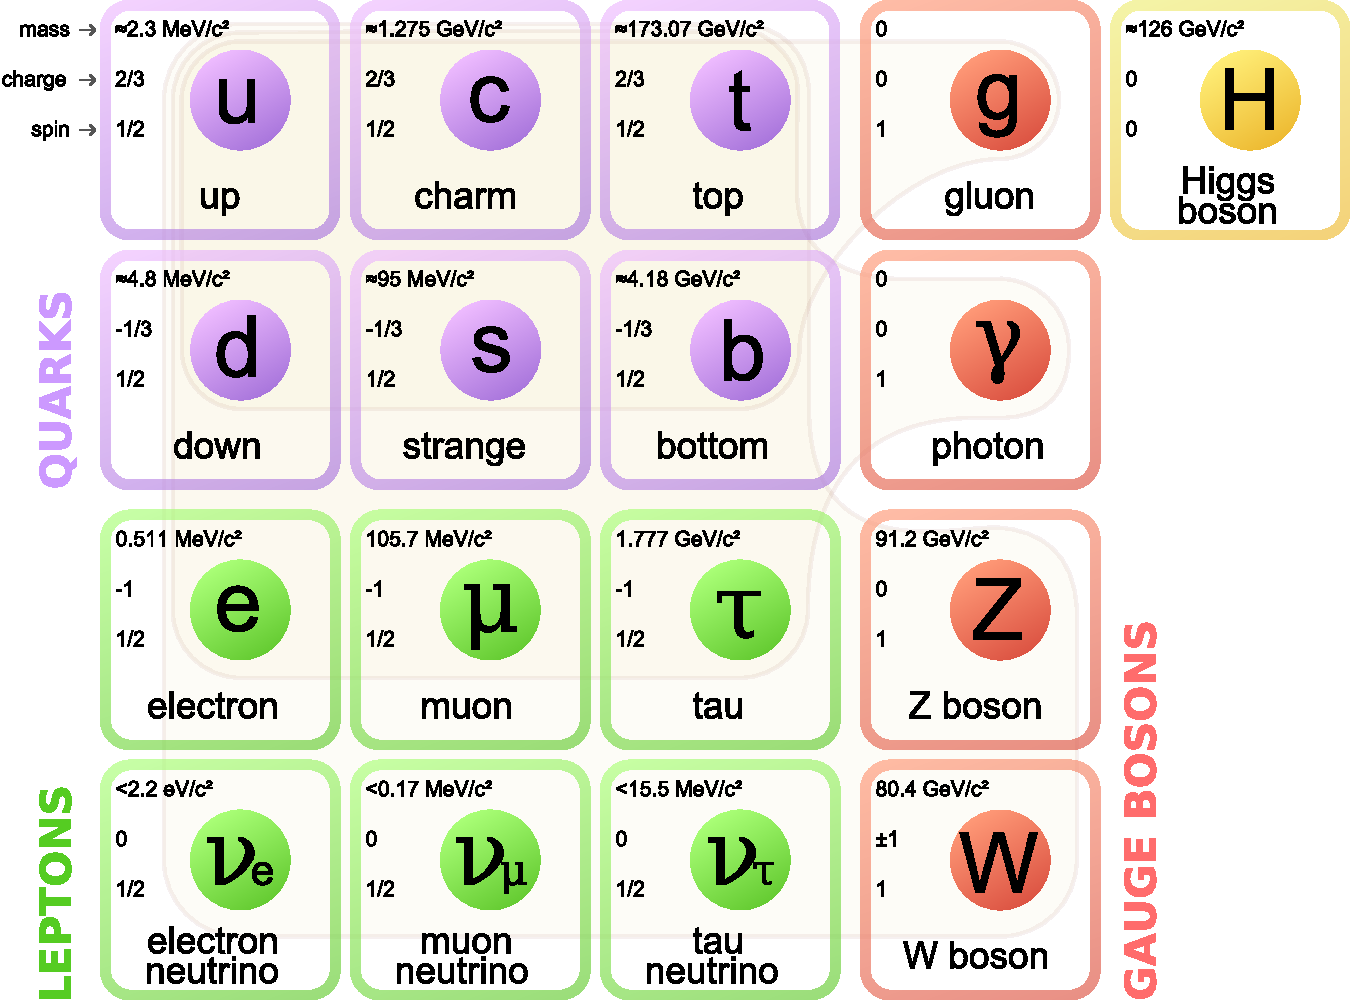
\includegraphics[width=0.8\textwidth]{figures/susyintro/Standard_Model_of_Elementary_Particles.pdf}
	\caption{An overview of the particles of the Standard Model and their interactions, from \cite{Wikimedia_SM_particles}.}
	\label{fig:SM_particles}
\end{figure}

The flavours of the quarks and leptons are conserved in the electromagnetic and strong interactions. For instance, a top quark cannot change into a charm or up quark by emission of a photon or gluon. The weak interaction enables the top quark to change into a bottom quark, or a tau lepton to change into a tau neutrino, through the emission of a charged $W$ boson. This would still seem to conserve the {\it generation} of quark or lepton, but breaking of generation is also made possible through the mechanism of {\it generation mixing}, quantified by the Cabibbo-Kobayashi-Maskawa (CKM) matrix for the case of quarks and the Pontecorvo-Maki-Nakagawa-Sakata (PMNS) matrix for the leptons. The PMNS mixing also explains the observed phenomenon of {\it neutrino oscillations}.

\section{Constructing the Lagrangian of the Standard Model}

The Standard Model is a quantum field theoretic model, and may be stated in terms of a Lagrangian density function $\mathcal{L}$. The guiding principle for constructing the Lagrangian is {\it gauge invariance}. Gauge degrees of freedom are physical degrees of freedom which are ``superflous'', in the sense that they do not have any observable consequences. An example is Maxwell's theory of electromagnetism, where the electromagnetic vector potential $A^\mu$ is undetermined up to the addition of a total derivative term $\partial^\mu \phi$. The gauge freedom is exploited by requiring that the Lagrangian, which determines the physical dynamics, does not change when the gauge degrees of freedom are varied, {\it i.e.}\ that it is gauge invariant. This invariance is related to conservation of physical quantities by Noether's theorem.

\section{The Lie groups of the Standard Model}

The Standard Model is based on gauge invariance under three Lie groups of quadratic matrices, the famous $U(1)_Y\times SU(2)_L\times SU(3)_C$. The number in the parenthesis gives the matrix dimension of the group. The symbols $S$ and $U$ stand for {\it special} and {\it unitary}, respectively. Unitary means that the matrices are unitary, and special means they have determinant 1. The groups are Lie groups, which means that they are continuous, and thus that any transformation of a group element may be constructed from infinitesimal transformations. The group elements, and the objects on which the group acts, may be given in several {\it representations}. In the case of matrix groups this means matrices and vectors of different dimension. For an $SU(n)$ group, the two most important representations are the {\it fundamental} representation, where the vectors have dimension $n$, and the {\it adjoint} representation, where the vectors have dimension $n^2-1$. In the Standard Model, the fermions transform in the fundamental representation, while the gauge bosons transform in the adjoint representation.

An element $G$ of an $SU(n)$ group may generally be written as\footnote{Here and in the following, repeated indices are summed over.} 
\begin{align}
	G = e^{i\alpha_a T_a},
\end{align}
where $T_a$ are the $n^2-1$ generators of the Lie algebra of the group. The generators themselves are in the fundamental representation represented by traceless complex $n\times n$ matrices -- for $SU(2)$, these are the Pauli matrices $\sigma_i$, and for $SU(3)$ they are the Gell-Mann matrices $\lambda_i$ -- and in the adjoint representation by the {\it structure coefficients} $f_{abc}$ as $(T_a)_{bc} = f_{abc}$. The structure coefficients are determined from the Lie algebra as
\begin{align}
	[T_a, T_b] = i f_{abc}T_c.
\end{align}

\section{Constructing a gauge theory}
The particle content of the Standard Model is input into the Lagrangian by inserting fermionic fields, {\it i.e.}\ Dirac spinor fields, and imposing the desired gauge invariance on these fields. The basic Dirac term, called the Dirac bilinear, for some spinor field $\psi$, is\footnote{We will, for what follows, set $\hbar = c = 1$.} 
\begin{align}
	\bar \psi (i\gamma^\mu \partial_\mu - m) \psi = \bar \psi (i\slashed\partial - m)\psi, \label{eq:diracbilinear}
\end{align}
where $\gamma_\mu$ are the Dirac matrices, $m$ is the mass of the spinor field, and $\bar\psi \equiv \psi^\dag \gamma_0$. Next, we impose gauge invariance. The group transformation of an $SU(n)$ group may be written in the fundamental representation as
\begin{align}
	G(x) = e^{ig\alpha_a(x)T^a},
\end{align}
where $\alpha(x)$ are $n$ arbitrary real differentiable functions and $T^a$ are the generators of $SU(n)$ in the fundamental representation. We assume that the Lagrangian consists of $n$ Dirac bilinear terms with fields $\psi_i$, and that they are put into an $n$-dimensional multiplet $\Psi = (\psi_1, \psi_2, ..., \psi_n)^T$ such that the basic Dirac Lagrangian reads
\begin{align}
	\mathcal{L}_0 = \bar\Psi(i\slashed\partial - m)\Psi
\end{align}
where we assume that all fields have the same mass $m$.\footnote{This assumption is often wrong in the case of the Standard Model, but finds its solution in the Higgs mechanism.} The group transformations of the multiplet and its adjoint are then 
\begin{align}
	\Psi(x) &\overset{G}{\to} e^{(ig\alpha_a(x)T^a)} \Psi(x),\\
	\bar\Psi(x) &\overset{G}{\to} \bar\Psi(x) e^{(-ig\alpha_a(x)T^a)}.\nonumber
\end{align}
If we apply these transformations to the basic Lagrangian, it becomes
\begin{align}
	\mathcal{L}_0 = &\bar\Psi(x)(i\slashed\partial - m)\Psi(x)\nonumber\\
	\overset{G}{\to} &\bar\Psi(x) e^{(-ig\alpha_a(x)T^a)}(i\slashed\partial - m)e^{(ig\alpha_a(x)T^a)} \Psi(x)\\
	=	&\bar\Psi(x)(i\slashed\partial - m)\Psi(x) - g\bar\Psi(x) T^a\slashed\partial \alpha^a(x) \Psi(x).\nonumber
\end{align}
Thus, the basic Dirac Lagrangian is not gauge invariant, since we have picked up an additional term. Gauge invariance may be achieved by adding a term of the form 
\begin{align}
	-\bar\Psi(x) ig\gamma^\mu \alpha_a(x)A^a_\mu(x) \Psi(x)\label{eq:covariantderivativeterm}
\end{align}
to the Lagrangian, where $A^a_\mu(x)$ is some new field, which we require to transform under $G$ as
\begin{align}
	A^a_\mu(x) \overset{G}{\to} A^a_\mu(x) + \partial_\mu \alpha^a(x).
\end{align}
If we apply $G$ to the sum of the Dirac bilinear with this new term, it is invariant:
\begin{align}
	&\bar\Psi(x)(i\slashed\partial - m)\Psi(x) - \bar\Psi(x) ig\gamma^\mu \alpha_a(x)A^a_\mu(x) \Psi(x)\nonumber\\
	\overset{G}{\to} &\bar\Psi(x)(i\slashed\partial - m)\Psi(x) - g\bar\Psi(x) T^a\slashed\partial \alpha^a(x) \Psi(x)\\
	 &- \bar\Psi(x) ig\gamma^\mu \alpha_a(x)A^a_\mu(x) \Psi(x) +  g\bar\Psi(x) T^a\slashed\partial \alpha^a(x) \Psi(x)\nonumber\\
	 = &\bar\Psi(x)(i\slashed\partial - m)\Psi(x) - \bar\Psi(x) ig\gamma^\mu \alpha_a(x)A^a_\mu(x) \Psi(x).\nonumber
\end{align}
The term from eq.\ \eqref{eq:covariantderivativeterm} is usually included by replacing $\partial_\mu$ with the {\it covariant derivative}
\begin{align}
	D_\mu = \partial_\mu + igT_a A^a_\mu.
\end{align}
The fields $A^a_\mu$ are called gauge boson fields, and are responsible for mediating interactions between the Dirac fermion fields. The gauge boson fields must also have their own free-field term in the Lagrangian, called the field strength, which is given from the Proca Lagrangian for spin-1 fields as 
\begin{align}
	-\frac{1}{4} F_{a,\mu\nu} F^{a,\mu\nu},
\end{align}
where
\begin{align}
	igT_a F_{a,\mu\nu} \equiv [D_{a,\mu}, D_{a,\nu}] = igT_a \left[ \partial^\mu A_a^\nu - \partial^\nu A_a^\mu + g f_{abc} A^{b,\mu}(x)A^{c,\nu}(x) \right],
\end{align}
where $f_{abc}$ are the structure coefficients of $SU(n)$.

With this, the total gauge invariant Lagrangian consists of $n$ fermion fields and $n^2-1$ gauge boson fields, and reads
\begin{align}
	\mathcal{L} = \bar\Psi(i\slashed D - m)\Psi - \frac{1}{4} F_{a,\mu\nu} F^{a,\mu\nu}.
\end{align}
The covariant derivative gives rise to terms coupling the fermion and gauge fields together. In the case of $n=1$, the gauge group is the $U(1)$ group, which describes the theory of quantum electrodynamics, the simplest realistic gauge theory. For $U(1)$, the structure coefficients vanish, since there is only a single gauge field\footnote{This contradicts the claim that there are $n^2-1$ gauge fields -- for $U(n)$ there are $n^2$ of them. The reason is that $U(1)$ is not an $SU(n)$ group, but the above derivation works for $U(1)$ as well.}, making the Lagrangian particularily simple. In QED, there are no gauge boson self-interactions. For $n>1$, the structure coefficients do not vanish, and this gives rise to terms in the field strength term $-\frac{1}{4} F_{a,\mu\nu} F^{a,\mu\nu}$ coupling the gauge bosons among themselves. These couplings are of great importance in the theories of weak and strong interactions.




\section{Singlets, doublets and triplets}

Not all the fields are subject to all the different interactions. If a field couples through a certain interaction, it is said to be {\it charged} under the transformations corresponding to that interaction. A specific amount $g$ of charge is assigned to every field, and enters into the group transformations as $G(x) = e^{ig\alpha_a(x)T^a}$. Thus, for $g=0$, the transformation is the identity and has no effect.  In the electromagnetic $U(1)$ case, this charge is the electrical charge, $g=q$. Analogous charges are associated with the $U(1)_Y$, $SU(2)_L$ and $SU(3)_C$ groups. They are called hypercharge, isospin and colour charge, respectively.

In the case of $SU(2)$ and $SU(3)$, the fields have to be put into vectors in order to be acted upon by the transformations, as was done in the previous section. Since the fermionic fields transform in the fundamental representation, the dimension of the vectors is 2 and 3, respectively. These types of vectors are referred to as $SU(2)$ {\it doublets} and $SU(3)$ {\it triplets}.

A Dirac field can be written as the sum of a left-chiral and a right-chiral part, defined by the projection operators 
\begin{align}
	P_{R/L} = \frac{1\pm \gamma^5}{2},
\end{align}
where $\gamma^5 \equiv i\gamma^0\gamma^1\gamma^2\gamma^3$. Given a Dirac field $\psi$, we may write
\begin{align}
	\psi = \left( \frac{1 + \gamma^5}{2} + \frac{1 - \gamma^5}{2}\right)\psi = P_R \psi + P_L \psi \equiv \psi_R + \psi_L.
\end{align}
In the case of $SU(2)_L$, only the {\it left chiral} part of the fields are charged under the symmetry. For instance, the left-chiral parts of the quark fields are put in doublets, {\it e.g.}\
\begin{align}
	q_L = \begin{pmatrix}
		u_L \\ d_L
	\end{pmatrix},
\end{align}
for the up- and down-quarks, while the right-handed parts of each of the quark fields are put in two separate singlets $u_R$ and $d_R$, upon which the $SU(2)_L$ transformation does not act. This has the consequence that the $SU(2)_L$ interaction is left-chiral -- it only couples to left-handed fields. Due to the spontaneous symmetry breaking of the $U(1)_Y\times SU(2)_L$ symmetry, the chirality is not exact in the resulting weak interactions, but it is still an important feature of the Standard Model.

The $SU(3)_C$ symmetry is the symmetry of the strong nuclear force, and among the fermions, only the quarks are charged under it. The quarks transform under $SU(3)$ in triplets -- one for each quark flavour -- where the components of the triplet are discriminated by differing {\it colour}, red, green or blue. 

\subsection{The gauge bosons and the adjoint representation}

While the fermions transform under the groups in the fundamental representation, which has dimension $n$ for $SU(n)$, the gauge vector boson fields transform in the adjoint representation, which has dimension $n^2-1$. This number then determines the number of different gauge bosons for each group: $U(1)_Y$ has a single gauge boson field labeled $B^\mu$; $SU(2)_L$ has three, labeled $W^\mu_{1,2,3}$; and $SU(3)_C$ has eight different gauge boson fields, labeled $A^\mu_a$ for $a = 1,...,8$. The $SU(3)$ bosons are called {\it gluons}. The $U(1)_Y$ and $SU(2)_L$ bosons are not the ones that we observe -- the physical gauge boson eigenstates are linear combinations of them, mixed together by the spontaneous symmetry breaking of the Higgs mechanism.

\section{The Higgs mechanism}
Gauge invariance forbids the inclusion of terms of the form $m^2A^\mu A_\mu$ into the Lagrangian, which are required in order to give vector bosons such as the $Z$ their observed mass. To include the terms, we must also include a new complex scalar field doublet $\Phi = (\phi_a^0, \phi_b^0)^T$. The Higgs mechanism introduces the following terms into the Lagrangian:
\begin{align}
	\mathcal L \ni |D_\mu \Phi(x)|^2 - \mu^2|\Phi(x)|^2 - \lambda |\Phi(x)|^4.
\end{align}
The last two terms comprise the Higgs {\it potential}. If $\mu^2$ is assumed to be negative and $\lambda$ positive, then the potential assumes the shape of a ``mexican hat'' as a function of $|\Phi|$. This is shown in fig. \ref{fig:higgspot}.
\begin{figure}[hbt]
	\centering
	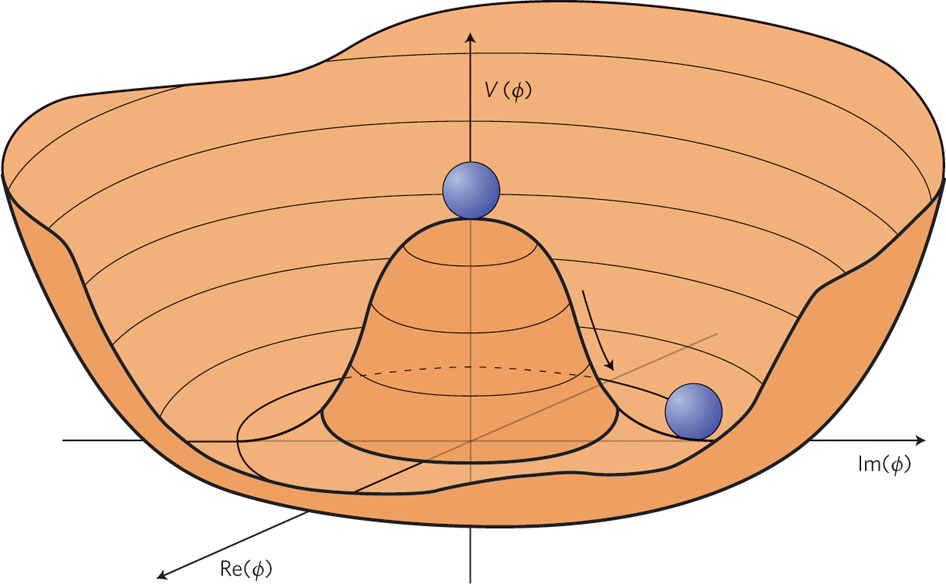
\includegraphics[width=0.5\textwidth]{figures/susyintro/higgspot_nature.jpg}
	\caption{The shape of the Higgs potential, from \cite{Ellis:higgs}}
	\label{fig:higgspot}
\end{figure}
This potential has a circle of degenerate energy at the field value $|\Phi|^2 = |\phi_a^0|^2 + |\phi_b^0|^2 = -\mu^2/2\lambda$. The mechanism of {\it spontaneous symmetry breaking} occurs when, as the energy decreases, the Higgs field falls to the bottom of the degenerate circle and is forced to {\it choose} a particular point on the circle. This causes $\Phi$ to obtain a {\it vacuum expectation value} (vev) $\langle \Phi \rangle = v$. This vacuum expectation value breaks the gauge invariance of the Lagrangian under both $U(1)_Y$ and $SU(2)_L$, and causes the gauge bosons of the two groups to mix together: The $B^\mu$ field mixes with $W^\mu_3$ to form the fields $A^\mu$ and $Z^\mu$, by the assignments
\begin{align}
	W_3^\mu &= \cos\theta_W Z^\mu + \sin\theta_W A^\mu,\\
	B^\mu &= -\sin\theta_W Z^\mu + \cos\theta_W A^\mu,
\end{align}
where $\theta_W$ is the {\it Weinberg angle}. The two other $SU(2)_L$ gauge fields, $W_{1,2}^\mu$, mix together to form
\begin{align}
	W^\mu = \frac{1}{\sqrt{2}} \left[ W_1^\mu - iW_2^\mu \right]
\end{align}
and its adjoint $(W^\mu)^\dag$. The field $A^\mu$ is the photon field, $Z^\mu$ is the Z boson field and $W^\mu/(W^{\mu\dag})$ is the $W^\pm$ bosons. The $Z$ and $W$ bosons acquire mass, the magnitude of which are related to $v$ by
\begin{align}
 	m_W = \frac{ve}{2\sin\theta_W},\\
 	m_Z = \frac{m_W}{\cos\theta_W},
\end{align}
where $e$ is the electromagnetic coupling constant, or the elementary unit of charge. The mixing of $U(1)_Y$ and $SU(2)_L$ restores the symmetry under a different $U(1)$ group, $U(1)_\mathrm{em}$, and the corresponding conserved charge is the electrical charge. The photon and Z boson are electrically netural, while the $W^\pm$ carry plus/minus one elementary unit of charge. Of the four degrees of freedom in the two complex scalar fields $\phi^0_{a,b}$, three go into providing the longitudinal polarization degree of freedom required for massive vector bosons, while the last one constitutes the {\it Higgs field} $h$.

The Higgs mechanism also provides fermionic terms of the form $\psi_i y_{ij} \psi_j$. For $i=j$, these are mass terms of the form written in the Dirac bilinear, eq. \eqref{eq:diracbilinear}, and for $i\neq j$ they give rise to off-diagonal terms in the CKM and PMNS matrices. The coupling constants of these terms are called {\it Yukawa couplings}.

\section{The Feynman calculus and loop corrections}
\label{subsec:feynmancalculus}
Very few problems in the framework of the Standard Model can be solved exactly. Instead, calculations are done using perturbation theory to series expand the solution as a sum of increasingly complicated, but decreasingly important, contributions. Feynman invented a technique for visualizing these expansions using diagrams, known as Feynman diagrams. For instance, the problem of inelastic electron-positron scattering has as its leading contribution the diagram shown in fig. \ref{fig:feynmandiagram_a}. The next-to-leading order includes the diagrams in figs. \ref{fig:feynmandiagram} (b), (c) and (d).
\begin{figure}[htbp]
	\centering
	\begin{subfigure}[b]{0.45\textwidth}
		\centering
		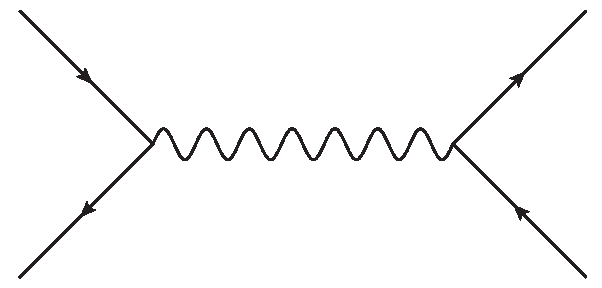
\includegraphics[width=0.6\textwidth]{figures/susyintro/epscattering.pdf}
		\caption{ }
		\label{fig:feynmandiagram_a}
	\end{subfigure}
	\begin{subfigure}[b]{0.45\textwidth}
		\centering
		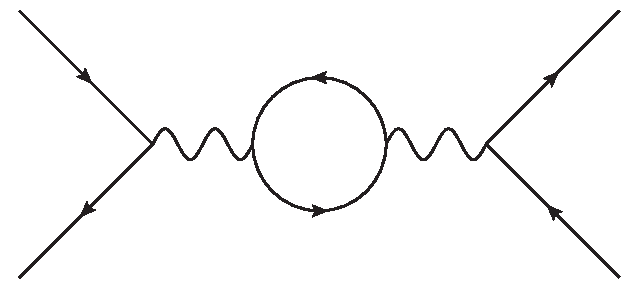
\includegraphics[width=0.6\textwidth]{figures/susyintro/epscattering_fermionloop.pdf}
		\caption{ }
		\label{fig:feynmandiagram_b}
	\end{subfigure}

	\begin{subfigure}[b]{0.45\textwidth}
		\centering
		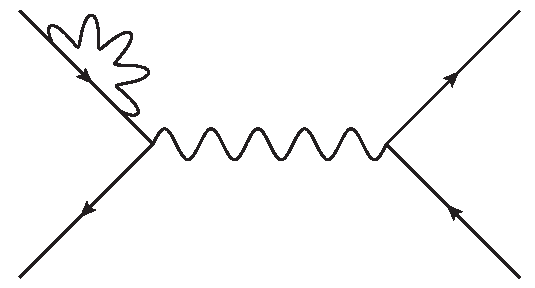
\includegraphics[width=0.6\textwidth]{figures/susyintro/epscattering_fermioncorr.pdf}
		\caption{ }
		\label{fig:feynmandiagram_c}
	\end{subfigure}
	\begin{subfigure}[b]{0.45\textwidth}
		\centering
		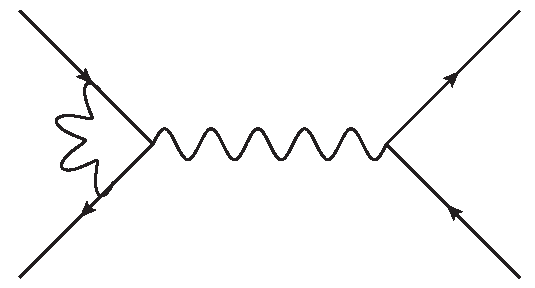
\includegraphics[width=0.6\textwidth]{figures/susyintro/epscattering_vertexcorr.pdf}
		\caption{ }
		\label{fig:feynmandiagram_d}
	\end{subfigure}
	\caption{Feynman diagrams of contributions to inelastic $e^+ e^-$ scattering. Made using \cite{Binosi:2003yf}.}
	\label{fig:feynmandiagram}
\end{figure}
The Feynman calculus associates each diagram with a specific mathematical expression called the Feynman amplitude $\mathcal{M}$ for that diagram. When several diagrams are included, the total amplitude for the process is the sum of the amplitudes from each diagram. The physical quantities of interest are obtained by integrating the amplitude (or its absolute square) over all spin and momentum configurations of the system.

\section{Renormalization}
The subleading diagrams, like those in fig.  \ref{fig:feynmandiagram} (b--d), contain closed loops. These loops introduce extra momentum integrals into the calculations. Often, these integrals are divergent -- which is unacceptable from a physical viewpoint. The divergences can be understood and dealt with by using the techniques of {\it regularization} and {\it renormalization}. 
\subsection{Regularization}
Regularization is a means for parametrizing the divergence in terms of some small parameter $\epsilon$ which is zero in the physical limit. The most modern way to regularize a momentum integral is by using {\it dimensional regularization}: The original loop integral is an integral over four space-time dimensions. Dimensional regularization makes the substitution $4 \to d = 4-\epsilon$, so the integral becomes
\begin{align}
	\int d^4 \, k \to \int d^d \, k.
\end{align}
This integral is mathematically well-defined, and allows the divergences to be parametrized in terms of $\epsilon$.
\subsection{Renormalization}
When the divergence has been isolated and parametrized, it needs to be explained physically. This is done by the process of renormalizing the theory. For instance, in the case of the photon propagator in quantum electrodynamics, illustrated in fig. \ref{fig:feynmandiagram_b}, the regularized expression for the leading-order loop correction to the propagator is proportional to
\begin{align}
	\frac{2}{\epsilon} + \mathrm{finite\,\, terms}, \label{eq:divergent_loop_result}
\end{align}
which blows up as $\epsilon\to 0$. Renormalization is the claim that this infinity is a part of the {\it bare} physical constants which are present in the Lagrangian, in this case the electrical charge, whose bare value is denoted $e_0$. These bare parameters are not observable quantities, only parameters in the Lagrangian. What is observed is the {\it renormalized} charge $e = e_0 + \delta e$, where $\delta e$ is the infinite shift contributed from eq. \eqref{eq:divergent_loop_result}.

All the coupling constants of the Standard Model get renormalized. The renormalization introduces an {\it energy dependence} into the coupling constants, since the shift comes from loop corrections which depend on the energy of the process. For instance, the physical value of the electron charge in quantum electrodynamics, at some momentum $q$, is given as
\begin{align}
	e^2(q) = \frac{e_r^2}{1 - (e_r^2/6\pi^2)\log(q/M)},\label{eq:electron_charge_running}
\end{align}
where $e_r$ is some referance value for the charge, defined at the energy scale $M$. The fact that the coupling constants are not constant is referred to as the {\it running of the coupling constants}.

\subsection{The Callan-Symanzik equation}
The Callan-Symanzik, or {\it renormalization group} equation (RGE) is the equation which describes the running of the coupling constants in a systematic way for any interaction in a quantum field theory. It is obtained by requiring that the Greens function for the interaction, $G$, {\it i.e.}\ the propagator, varies with the renormalization scale $M$ in such a way that the bare parameters of the Lagrangian is unchanged. For the example of QED, the Callan-Symanzik equation for a Green's function with $n$ electron fields and $m$ photon fields is
\begin{align}
	\left[ M \frac{\partial}{\partial M} + \beta(e) \frac{\partial}{\partial e} + n\gamma_2(e) + m\gamma_3(e)\right] G^{(n,m)}(\{ x_i\}; M,e) = 0.\label{eq:callansymanzik}
\end{align}
The functions $\beta$ and $\gamma$ are defined as
\begin{align}
	\beta \equiv \frac{M}{\delta M} \delta e, \, \gamma_i \equiv - \frac{M}{\delta M}\delta \eta_i,
\end{align}
where $\delta\eta_i$ is the field-strength renormalization term, shifting the field values of the electron and photon fields,
\begin{align}
	\psi \to (1 + \delta \eta_2) \psi \, \mathrm{and} \, A_\mu \to (1 + \delta\eta_3) A_\mu,
\end{align}
respectively. The Callan-Symanzik equation states that the combined effect of all the shifts in parameters induced by the renormalization should exactly weigh up for the shift in the Green's function itself, which is given by
\begin{align}
	G^{(n,m)} \to (1 + n\delta\eta_2 + m\delta\eta_3)G^{(n,m)}.
\end{align}
This is what is stated in eq.\ \eqref{eq:callansymanzik}. The Callan-Symanzik equation for other interactions, such as the $SU(3)$ quantum chromodynamics, may be derived similarily, but its complexity grows with the complexity of the interaction.

The primary quantities of interest from a phenomenological viewpoint are the $\beta$ and $\gamma$ functions. They describe the change in the coupling constant and other parameters as a function of renormalization scale, and in the case of QED they may be used to derive the formula \eqref{eq:electron_charge_running} for the running of the electromagnetic coupling constant $e$. Equation \eqref{eq:electron_charge_running} shows that the electromagnetic coupling constant increases as a function of the energy $q$. The same turns out to be true for the weak coupling constant, while the strong coupling constant of QCD decreases with increasing energy. This last fact is called {\it asymptotic freedom}, and means that the quarks and gluons are unbound by strong forces in the limit of high energy. 





\section{Motivations for extending the Standard Model}

Since the Standard Model is widely believed to be a low-energy effective model of some more fundamental high-energy regime, it is speculated that the three interactions of the Standard Model unite at a higher energy and act as a single interaction under some larger gauge group. However, when the three couplings are evolved to high energies using the Callan-Symanzik equations, they do not meet at a single point. This is seen by many as a flaw of the Standard Model. In the theory of Supersymmetry, the evolution of the couplings is altered, and they do meet at a single point. This is shown in fig. \ref{fig:coupling_unification}. Supersymmetry is discussed in detail in the next chapter.
\begin{figure}[hbt]
	\centering
	\includegraphics[width=0.6\textwidth]{figures/susyintro/unification.eps}
	\caption{Evolution of the inverse coupling constants, for the cases of the Standard Model (dashed lines) and models with supersymmetry (solid lines). From \cite{Martin:1997ns}.}
	\label{fig:coupling_unification}
\end{figure}

Another issue with the Standard Model is that is has no candidate for particle dark matter. Observations over the last century have given strong evidence for the existence of some as yet unkown form of matter which is distributed in large quantites all over the universe -- in fact four times as much as our ordinary matter. It is widely believed that this dark matter is some form of particle. Dark matter interacts primarily, or possibly even solely, via gravitation, so the particle has to be colourless and electrically neutral, because the strength of these interactions would otherwise lead to the particle having been observed by now. It also has to be long-lived in order to explain the abundance of dark matter that we observe in the universe today, because the assumption is that it was thermally produced in the early universe and subsequently cooled off. These restrictions rule out most of the Standard Model particles, with the exception of neutrinos. But neutrinos are known to be very light, almost massless, and calculations of early-universe dynamics show that they are too light to be candidates for dark matter. 

There is also a more technical problem with the Standard Model, related to the scalar Higgs field. As discussed in section \ref{subsec:feynmancalculus}, the calculations of parameters in a quantum field theory are subject to loop corrections. The Higgs mass parameter recieves corrections from loops containing all massive particles, with the largest contribution coming from the top quark. These contributions are many orders of magnitude larger than the observed Higgs mass of 126 GeV, meaning that there must be cancellations among the correction terms. There is no symmetry in the Standard Model which says that such a cancellation should occur, so it appears to be an ``accident'' of nature. Such accidents are seen as very unnatural, and this explanation is thus very unsatisfactory from a theoretical viewpoint. This is called the {\it hierarchy problem}. In supersymmetry, the new degrees of freedom enter into the loop corrections, and because of the symmetry, they cancel the Standard Model contributions in a natural way. 



% The Standard Model is a quantum field theoretic model and may be stated in terms of a Lagrangian density function $\mathcal{L}$. The features that define the Standard Model emerge by requiring that it is invariant under the action of certain {\it gauge groups} -- specifically the infamous $U(1)_Y\times SU(2)_L\times SU(3)_C$, where the subscripts stand for {\it hypercharge, left} and {\it colour}, respectively, and refer to the properties that the different fields must have in order to be acted upon by the group transformations. By inserting certain {\it fermionic} field content in the Lagrangian and imposing these symmetries, the model acquires a number of {\it gauge bosons} for the different gauge groups. All these particles are {\it a priori} massless, a requirement to fulfill the gauge symmetry. To give particles their observed mass, then, one adds a scalar field and a corresponding scalar potential of a certain shape. The shape of the potential is such that the $U(1)_Y\times SU(2)_L$ symmetry is {\it spontaneously broken} at a certain energy scale, shifting the degrees of freedom around to give a scalar Higgs boson along with the other gauge bosons, and also giving mass to all particles except the photon. The remaining unbroken symmetries are then the $U(1)_\mathrm{em}$ for electromagnetic and $SU(3)_C$ for strong interactions. 



% The particles that make up the Standard Model are: the three generations of charged leptons, electron, muon and tau, and their three neutral counterparts, the neutrinos; the three generations of up- and down-type quarks up, down, charm, strange, top and bottom; the electroweak gauge bosons photon, Z and W; the strong gauge bosons, the gluons; and the Higgs boson. 





%%%%%%%%%%%%%%%%%%%%%%%%%%%%%%%%%%%%%%%%%%%%%%%%%%%%%%%%%%%%%%%%%%%%%%%%
\chapter{Supersymmetry}%%%%%%%%%%%%%%%%%
%%%%%%%%%%%%%%%%%%%%%%%%%%%%%%%%%%%%%%%%%%%%%%%%%%%%%%%%%%%%%%%%%%%%%%%%
\label{ch:susyintro}
The theory of supersymmetry (SUSY) is a proposed extension of the Standard Model which increases the number of degrees of freedom by introducing a symmetry between fermions and bosons, called a supersymmetry. The construction of supersymmetry is in some sense a two-step process, where one first derives the Lagrangian of a theory with complete symmetry between fermions and bosons, meaning that every bosonic degree of freedom gets a corresponding `supersymmetric' fermionic degree of freedom, and {\it vice versa}. These fields only differ in spin. But since {\it e.g.}\ scalar, colour charged particles with the same mass as the quarks are not observed in experiments, the symmetry cannot be exact. To make the theory physically viable, the supersymmetric partners must be significantly heavier than their Standard Model counterparts. This means that the supersymmetry must be a broken symmetry, and this breaking is put into the theory ``by hand''.

In this chapter we will outline the construction of a supersymmetric theory. First, we introduce the group theoretic framework of the symmetries. We define the concept of superfields, fields transforming under representations of the supersymmetry group. We go on to construct a fully supersymmetric Lagrangian in the framework of the Minimal Supersymmetric Standard Model (MSSM). Then the breaking of SUSY is achieved by manually inserting so-called ``soft'' SUSY-breaking terms. Also, the concept of R-parity is introduced in order to ensure the stability of the proton. R-parity will also make the lightest supersymmetric particle a good dark matter candidate. From the broken SUSY Lagrangian, we extract the particle content -- identifying the familiar fields of the Standard Model as well as their supersymmetric counterparts. We then introduce popular phenomenological models used to constrain and study the parameter space of the MSSM, and discuss their implications for the hierarchy of SUSY masses. This type of constrained model is subsequently adapted for the study of particular chain decays, which is the topic for the remainder of the thesis. We will also review the current experimental status of SUSY. 

The presentation is based on \cite{Batzing:2013} and \cite{Leinonen:2014}.

\section{Extending the Poincar\'{e} symmetry}
In the beginning of Chapter \ref{ch:SM_intro}, the Poincar\'{e} group was discussed. It is the group of all Lorentz boosts and rotations, as well as all translations in spacetime. Any physical theory obeying Special Relativity must be invariant under the Poincar\'{e} group. It was shown in 1967 by Coleman and Mandula \cite{PhysRev.159.1251} that there exists no extension of the Poincar\'{e} symmetry which includes the gauge groups of the Standard Model in a non-trivial way, {\it i.e.}\ a way by which the extended group cannot be decoupled as a direct product such that the groups do not couple to each other. 

This prompted Haag, \L{}opusza\'{n}ski and Sohnius \cite{Haag1975257} to introduce the concept of a {\it superalgebra}. A superalgebra is a direct product of two Lie algebras with a binary operation that mixes the algebras together. Haag {\it et.al.}\ constructed a superalgebra by combining the Lie algebra of the Poincar\'{e} group with an algebra spanned by four operators called {\it Majorana spinor charges}, represented by a two-component Weyl spinor $Q_A$ (to be defined shortly) and its hermitian conjugate $\bar Q_{\dot A}$. The resulting superalgebra is given by the (anti)commutation relations
\begin{align}
	[Q_A,P_\mu] =& [\bar Q_{\dot A}] = 0,\\
	[Q_A, M_{\mu\nu}] =& \sigma_{\mu\nu,A}^B Q_B,\\
	\{Q_A, Q_B\} =& \{\bar Q_{\dot A}, \bar Q_{\dot B} \} = 0,\\
	\{Q_A, \bar Q_{\dot B} \} =& 2\sigma^\mu_{A \dot B} P_\mu,\\
\end{align}
where $P_\mu$ is the momentum operator (the generator of translations in the Poincar\'{e} group), $M_{\mu\nu}$ are the generators of Lorentz boosts and rotations, $\sigma_\mu = (1,\sigma_i)$ with $\sigma_i$ the Pauli matrices and $\sigma_{\mu\nu} = \frac{i}{4}(\sigma_\mu \bar\sigma_\nu - \sigma_\nu \bar\sigma_\mu)$. 

In the usual representation of the Poincar\'{e} group, the fermion fields are represented as four-component Dirac spinors. It can be shown that the Poincar\'{e} group is isomorphic to $SL(2,\mathbb{C})$, so it is possible to work with representations of this group instead. The $SL(2,\mathbb{C})$ group has two inequivalent fundamental representations by two-component spinors which are called {\it left- and right-handed Weyl spinors} and written as $\psi_A$ and $\bar\psi_{\dot A}$, respectively. 

The transformations corresponding to the superalgebra are called {\it supersymmetry transformations}.

\section{Superfields}
The representations of the objects transforming under the supersymmetry transformations are called superfields. There are two important types, called chiral/scalar and vector superfields. The superfields are expressed in terms of spacetime coordinates $x^\mu$ and four anti-commuting Grassman numbers $\theta_A$ and $\bar\theta_{\dot A}$. Together, these eight coordinates form the {\it superspace}. Because of the anticommutativity, which means that any Grassman number squared vanishes, a function of a Grassman number, $f(\theta_A)$, has an all-order expansion given by
\begin{align}
	f(\theta_A) = a + b\theta_A.
\end{align}
Using this fact, a superfield $\Phi$ may generally be written as
\begin{align}
	\Phi = &f(x) + \theta^A\phi_A(x) + \bar\theta_{\dot A}\bar\chi^{\dot A}(x) + \theta \theta m(x)\\
	 &+ \bar\theta \bar\theta n(x) + \theta\sigma^\mu \bar\theta V_\mu(x) + \theta\theta\bar\theta_{\dot A}\bar\lambda^{\dot A}(x) + \bar\theta \bar\theta \theta^A \psi_A(x) + \theta \theta \bar\theta \bar\theta d(x).\nonumber
\end{align}
The different field components have the following properties: $f(x)$, $m(x)$ and $n(x)$ are complex (pseudo)scalars, $\psi_A(x)$ and $\phi_A(x)$ are left-handed Weyl spinors, $\bar\chi^{\dot A}(x)$ and $\bar\lambda^{\dot A}(x)$ are right-handed Weyl spinors, $V_\mu (x)$ is a Lorentz four-vector and $d(x)$ is a complex scalar.
% \begin{itemize}
% 	\item $f(x), m(x)$ and $n(x)$ are complex (pseudo)scalars
% 	\item $\psi_A(x)$ and $\phi_A(x)$ are left-handed Weyl spinors
% 	\item $\bar\chi^{\dot A}(x)$ and $\bar\lambda^{\dot A}(x)$ are right-handed Weyl spinors
% 	\item $V_\mu (x)$ is a Lorentz four-vector
% 	\item $d(x)$ is a complex scalar
% \end{itemize}

 A set of covariant derivatives are defined by
\begin{align}
	D_A = \frac{\partial}{\partial \theta^A} - i\sigma^\mu_{A \dot A}\bar\theta^{\dot A}\partial_\mu, \, \bar D^{\dot A} = -\frac{\partial}{\partial \bar \theta_{\dot A}} + i\bar\sigma^{\mu,A \dot A}\theta_A \partial_\mu.
\end{align}
In terms of these, a {\it left chiral} superfield $\Phi$ is defined by the condition.
\begin{align}
	\bar D^{\dot A} \Phi = 0.
\end{align}
By substituting $y^\mu = x^\mu - i\theta\sigma^\mu \bar \theta$, the covariant derivative $\bar D^{\dot A}$ is given as
\begin{align}
	\bar D^{\dot A} = -\frac{\partial}{\partial \bar\theta_{\dot A}}.
\end{align}
This shows that a left-chiral superfield must be independent of $\bar \theta$ in these coordinates, so it may generally be written as
\begin{align}
	\Phi(y, \theta) = A(y) + \sqrt{2}\theta\psi(y) + \theta\theta F(y), 
\end{align}
thus containing two complex scalar fields and a left-handed Weyl spinor. Under an infinitesimal supersymmetry transformation
\begin{align}
	\delta_\xi \Phi = -i(\xi Q + \bar\xi\bar Q)\Phi,
\end{align}
the component field $F$ can be shown to transform into a total derivative. It will thus not contribute to the action, since all fields must vanish on the boundary at infinity. For this reason it is called an auxillary field. Thus we see that a left-chiral superfield contains two bosonic (scalar) degrees of freedom and two fermionic degrees of freedom contained in a left-handed Weyl spinor. Similar arguments may be applied to define a right-chiral superfield by the condition
\begin{align}
	D_A \Psi^\dag = 0,
\end{align}
and to show that it contains two auxillary and two proper scalar degrees of freedom, as well as a right-handed Weyl spinor. 

A {\it vector superfield} is defined by the condition
\begin{align}
	\Phi^\dag = \Phi.
\end{align}
This condition allows the field content, for a general vector superfield $V$,
\begin{align}
	V = &f(x) + \theta^A\phi_A(x) + \bar\theta_{\dot A}\bar\chi^{\dot A}(x) + \theta \theta m(x) + \bar\theta \bar\theta m^*(x)\\
	 &+ \theta\sigma^\mu \bar\theta V_\mu(x) + \theta\theta\bar\theta_{\dot A}\bar\lambda^{\dot A}(x) + \bar\theta \bar\theta \theta^A \lambda_A(x) + \theta \theta \bar\theta \bar\theta d(x).
\end{align}
Here, the scalar fields $f(x)$ and $d(x)$, as well as the four-vector $V_\mu (x)$, are required to be real fields, thus halving their amount of degrees of freedom. There are auxillary degrees of freedom which may be removed by a gauge transformation. A vector superfield may be written in the {\it Wess-Zumino} gauge as
\begin{align}
	V_\mathrm{WZ} = (\theta \sigma^\mu \bar\theta) \left[ V_\mu(x) + i\partial_\mu (A(x) - A^*(x)) \right] + \theta\theta \bar\theta_{\dot A} \bar\lambda^{\dot A}(x) + \bar\theta \bar\theta \theta_A \lambda^A(x) + \theta\theta \bar\theta \bar\theta d(x).
\end{align}
In this gauge, the vector superfield contains one real scalar field degree of freedom (d.o.f.), three gauge field d.o.f.'s and four fermion d.o.f.'s.

\section{The unbroken SUSY Lagrangian}
To obtain a theory which is supersymmetric, the action, given by
\begin{align}
 	S = \int d^4 x \mathcal{L},
 \end{align}
 needs to be invariant under SUSY transformations. As mentioned in the previous section, a total derivative has this property because its integral is determined by the boundary conditions, where it has to vanish. It can be shown that the highest-order component fields in $\theta$ and $\bar \theta$, {\it i.e.}\ the term proportional to $\theta\theta\bar\theta\bar\theta$, always has this property for both chiral and vector superfields and products thereof. Thus the invariance of the action may be ensured by redefining the Lagrangian such that
 \begin{align}
 	S = \int d^4 x \int d^4 \theta \mathcal{L},
 \end{align}
 where the last integral is over the four Grassman variables. This will project out only the desired terms, because of how the Grassman integral is defined. Thus the supersymmetric Lagrangian may be constructed from superfields and their products.

 A {\it superpotential} is defined as a product of left-chiral superfields,
 \begin{align}
 	W(\Phi) = L^i\Phi_i + \frac{1}{2}m^{ij}\Phi_i\Phi_j + \frac{1}{3}\lambda^{ijk}\Phi_i\Phi_j\Phi_k.
 \end{align}
The inclusion of higher-order field terms are forbidden from the condition of renormalizability, which forbids terms where the combined mass dimension of the fields are larger than four. Scalar, fermionic and auxillary fields have mass dimension one, 3/2 and 2, respectively. A fourth order superfield term would include field terms which break this condidtion. The most general Lagrangian that can be written in terms of chiral superfields is
\begin{align}
	\mathcal{L} = \Phi_i^\dag \Phi_i + \bar\theta\bar\theta W(\Phi) + \theta\theta W(\Phi^\dag),
\end{align}
where the first term is called the kinetic term. 

The Lagrangian has to be gauge invariant. The general gauge transformation of a chiral superfield under a group $G$ is given by
\begin{align}
	\Phi \overset{G}{\to} e^{-iq\Lambda^a T_a}\Phi
\end{align}
where $T_a$ are the group generators, $q$ is the charge of $\Phi$ under $G$ and the gauge parameters $\Lambda_a$ themselves can be shown to be left-chiral superfields. The equivalent transformation for a right-chiral superfield $\Phi^\dag$ involves a right-chiral superfield gauge parameter $\Lambda_a^\dag$.

Analogously to the Standard Model, the supersymmetric gauge interactions are introduced as compensating terms to the gauge transformation of the chiral superfields. The analogue to the gauge boson fields are the vector superfields $V^a$, which are introduced into the kinetic terms of the Lagrangian by writing them as
\begin{align}
	\Phi^\dag_i e^{q V^a T_a}\Phi_i,
\end{align}
such that the kinetic term transforms as
\begin{align}
	\Phi_i^\dag e^{q V^a T_a}\Phi_i \overset{G}{\to} \Phi^\dag e^{iq(\Lambda^a)^\dag T_a}e^{qV^{'a}T_a}e^{-iq\Lambda^a T_a}\Phi,
\end{align}
which is invariant given that the vector superfields transform as
\begin{align}
	e^{qV^{'a} T_a} = e^{-iq(\Lambda^a)^\dag T_a}e^{qV^a T_a}e^{iq\Lambda^a T_a}.
\end{align}
For infinitesimal $\Lambda$, this is to leading order
\begin{align}
	V^{'a} = V^a + i(\Lambda^a - (\Lambda^a)^\dag) - \frac{1}{2}qf^a_{bc} V^b ((\Lambda^c)^\dag + \Lambda^c).
\end{align}
This gives for the vector component fields of the vector superfields, $V_\mu^a$,
\begin{align}
	V^a_\mu \overset{G}{\to} V^{'a}_\mu = V_\mu^a + i\partial_\mu(\Lambda^a - (\Lambda^a)^\dag) - qf^a_{bc} V_\mu^b (\Lambda^c + (\Lambda^{c})^\dag).
\end{align}
With these definitions, it can be shown that the Standard Model couplings of fermions with bosons are recovered by defining the covariant derivative
\begin{align}
	D_\mu^i = \partial_\mu - \frac{i}{2} q_i V_\mu.
\end{align}

The SUSY Lagrangian terms containing the field strengths of the gauge fields are written as
\begin{align}
	\mathrm{Tr}[W^A W_A],
\end{align}
called the supersymmetric field strength, where $W_A$ and $\bar W_{\dot A}$ are left- and right-handed chiral superfields, respectively, given by
\begin{align}
	W_A &\equiv -\frac{1}{4}\bar D\bar D e^{-qV^aT_a} D_A e^{qV^a T_a},\\
	\bar W_{\dot A} &\equiv -\frac{1}{4} D D e^{-qV^aT_a} \bar D_{\dot A} e^{qV^a T_a}.
\end{align}
The general form of the SUSY Lagrangian is
\begin{align}
	\mathcal{L} \Phi^\dag e^{qV^a T_a}\Phi + \bar\theta\bar\theta W(\Phi) + \theta\theta W(\Phi^\dag) + \frac{1}{2T(R)}\bar\theta \mathrm{Tr}(W^A W_A),
\end{align}
where $T(R)$, the {\it Dynkin index} of the representation of the gauge group, is a normalization constant.



\subsection{SUSY breaking}
Supersymmetry has to be a broken theory, at least in the low-energy limit, since supersymmetric particles with Standard Model masses are not observed. The breaking can be inserted into the SUSY Lagrangian ``by hand'', by explicitly adding terms that break SUSY and allow for mass splitting. The rationale for these terms is that the SUSY Lagrangian is only an effective Lagrangian where some heavy field has been integrated out, and that the breaking of SUSY occurs through this field at a higher scale. There are several alternatives for the mechanisms of SUSY breaking, some of which are Planck-scale mediated SUSY breaking, gauge mediated SUSY breaking and anomaly mediated SUSY breaking. Whichever of the mechanisms is chosen, there are only a finite set of terms that may be added to the Lagrangian without breaking renormalizability. They are called {\it soft} SUSY breaking terms, required to have couplings of mass dimension one or higher, and may in the most general form be written
\begin{align}
	\mathcal{L}_\mathrm{soft} = &-\frac{1}{4T(R)}M\theta\theta\bar\theta\bar\theta \mathrm{Tr} [W^A W_A] - \frac{1}{6}a_{ijk} \theta\theta\bar\theta\bar\theta\Phi_i \Phi_j \Phi_k\nonumber\\
	&-\frac{1}{2}b_{ij} \theta\theta\bar\theta\bar\theta\Phi_i \Phi_j - t_i \theta\theta\bar\theta\bar\theta \Phi_i + \mathrm{h.c.}\\
	&-m_{ij} \theta\theta\bar\theta\bar\theta \Phi_i^\dag \Phi_j.\nonumber
\end{align}
In terms of the component fields of the superfields, the soft Lagrangian may be written
\begin{align}
	\mathcal{L}_\mathrm{soft} = &-\frac{1}{2} M\lambda^A\lambda_A - \left( \frac{1}{6} a_{ijk} A_i A_j A_k + \frac{1}{2} b_{ij} A_i A_j + t_i A_i + \frac{1}{2} c_{ijk} A^*_i A_j A_k + \mathrm{c.c.}\right)\\
	&- m_{ij}^2 A_i^* A_j.\nonumber
\end{align}
Since this contains both Weyl spinor fields and scalar fields, the soft terms may be used to modify masses and couplings of the superpartner scalar and fermionic fields which will appear in a moment.



\section{The Minimal Supersymmetric Standard Model}
The Minimal Supersymmetric Standard Model (MSSM) is the minimal supersymmetric theory which contains the Standard Model. It is constructed by choosing field content in accordance with the requirements deduced in the previous sections. To construct a Dirac fermion, we use one left-chiral and one right-chiral superfield together. This gives the four fermionic degrees of freedom that a Dirac fermion and its antiparticle require. Since each chiral superfield also contains two scalar degrees of freedom (after removing the auxillary fields), this introduces two scalar particle-antiparticle pairs, which are called the supersymmetric partners, or {\it superpartners}, of the Dirac fermion. An important point is that all superfield components must have the same charge under all gauge groups, due to the way the gauge transformation was defined. This means that the scalar fields generally will be charged. For instance, the superfields for the charged leptons are denoted $l_i$ and $\bar E_i$ for the left- and right-chiral superfields, respectively, and the left-handed neutrino superfields are denoted $\nu_i$. Here, $i=1,2,3$ is a generation index. The $SU(2)_L$ doublet of the Standard Model is recovered by setting $L_i = (\nu_i, l_i)$. The quark superfields are denoted $u_i$, $\bar U_i$, $d_i$ and $\bar D_i$, where $Q_i = (u_i, d_i)$ makes the $SU(2)_L$ doublet.

The gauge boson fields come from the vector superfields, each of which also contains two Weyl-spinor fields of opposite handedness. To obey gauge invariance, $n^2-1$ vector superfields are required for each of the $SU(n)$ groups just as in the Standard Model -- {\it i.e.}\ gauge invariance under $U(1)_Y\times SU(2)_L \times SU(3)_C$ requires 1+3+8 vector superfields.\footnote{Again, $n^2$ rather than $n^2-1$ for the $U(1)$ group.} These are denoted $B^0$, $W^a$ and $C^a$, respectively. The Weyl spinor fields, corresponding to superpartners of the gauge fields, are written as $\tilde B^0$, $\tilde W^0$ and $\tilde g$, respectively. In the literature, these are referred to as {\it bino}, {\it wino} and {\it gluino}. 

The MSSM requires two Higgs superfield $SU(2)_L$ doublets to be able to give mass to both up- and down-type quarks. In the Standard Model, the same Higgs doublet can be used for both types by rotating the components using the $SU(2)_L$ generators, but this is not possible in SUSY. The Higgs doublets in the MSSM are
\begin{align}
	H_u = \begin{pmatrix}
		H_u^+ \\ H_u^0
	\end{pmatrix}, \, H_d = \begin{pmatrix}
		H_d^0 \\ H_d^-
	\end{pmatrix}.
\end{align}
This introduces several additional Higgs scalars into the model, as well as the fermionic superpartner fields.

The fields listed above come together and construct the MSSM Lagrangian $\mathcal{L}_\mathrm{MSSM}$ using the rules described above for a general gauge invariant SUSY Lagrangian, giving rise to kinetic terms, superpotential terms and supersymmetric field strength terms. The SUSY breaking soft terms of the MSSM are, in component fields,
\begin{align}
	&\left( -\frac{1}{2}M_1 \tilde B \tilde B - \frac{1}{2}M_2 \tilde W^{i,A} \tilde W^i_A - \frac{1}{2}M_3 \tilde g^{a,A}\tilde g^a_A + \mathrm{c.c.} \right)\nonumber\\
	+ &\left(-a_{ij}^e \tilde L_i H_d {\tilde e^*}_{iR} - a_{ij}^u \tilde Q_i H_u \tilde u^*_{iR} - a_{ij}^d \tilde Q_i H_d \tilde d^*_{jR} + \mathrm{c.c.} \right)\\
	- &(m_{ij}^L)^2 \tilde L_i^\dag \tilde L_j - (m_{ij}^e)^2 {\tilde e_{iR}^*} {\tilde e_{jR}} - (m_{ij}^Q)^2 \tilde Q_i^\dag \tilde Q_j \nonumber \\
	- &(m_{ij}^u)^2 {\tilde u_{iR}^*} {\tilde u_{jR}} - (m_{ij}^d)^2 {\tilde d_{iR}^*} {\tilde d_{jR}} - m^2_{H_u} H^\dag_u H_u - m^2_{H_d} H^\dag_d H_d.\nonumber
\end{align}
These terms constitute the main contributions to the superpartner masses.

The Lagrangian will {\it a priori} contain terms which break lepton and baryon number conservation, such as $LH_u$, $LLE$ and $LQ\bar D \in \mathcal{L}_\mathrm{MSSM}$. If the couplings for these terms are large, they allow for proton decay, which is experimentally very heavily constrained, with a lifetime of $\tau_\mathrm{proton} > 10^{33} \,\mathrm{yr}$. To avoid this, it is conventional to introduce the concept of {\it R-parity}, which gives an explanation for why these terms are zero.

\subsection{R-parity}
R-parity is a multiplicative quantum number which is assumed to be conserved in all SUSY interactions. Formally, a particle has R-parity given by
\begin{align}
	R = (-1)^{2s + 3B + L},
\end{align}
where $s$ is the particle's spin, $B$ its baryon number and $L$ its lepton number. The important point is that all Standard Model particles have $R=+1$ while all superpartners have $R = -1$. This leads to the very important prediction that superpartner particles only can be produced and annihilated in pairs. In particular, it means that the lightest superpartner (LSP) must be stable against decay. This makes the LSP very attractive as a candidate for dark matter, if it is electrically neutral.

\subsection{Radiative electroweak symmetry breaking}
Like any quantum field theory, the MSSM is subject to renormalization, which induces the running of the coupling constants and masses of the model as discussed in Chapter \ref{ch:SM_intro}. In particular, the mass parameters $m_{H_u/d}$ for the Higgs doublets, which come from soft breaking terms in the Lagrangian, run with energy. To break the electroweak symmetry, it is assumed that these are equal at some high scale, and run down. It can be shown that the running is proportional to the Yukawa couplings of the third-generation quarks of the respective type -- {\it i.e.}\ the top and bottom, respectively. Because the top Yukawa coupling is much larger than the bottom one, the $m_{H_u}$ parameter runs down much faster with energy and becomes negative. One can further show that this is a sufficient condition to induce the electroweak symmetry breaking, and thus give the gauge bosons and fermions their observed mass.\marginpar{Is this too ``dodgy''? Should I be more technical? I fear there are too many technicalities already.} 

In the course of the symmetry breaking, the neutral components of both the Higgs doublets acquire a non-vanishing vacuum expectation value, $v_u = \langle H_u^0 \rangle$ and $v_d = \langle H_d^0 \rangle$, respectively. These must relate to the vector boson masses of the Standard Model as
\begin{align}
	v_u^2 + v_d^2 = \frac{2m_Z^2}{g^2 + g^{'2}} \approx (174 \,\mathrm{GeV})^2.
\end{align}
The remaining free parameter is conventionally parametrized as
\begin{align}
	tan \beta \equiv \frac{v_u}{v_b}.
\end{align}

\subsection{Particle phenomenology of the MSSM}
The total particle content of the MSSM is as follows: 
\begin{itemize}
	\item The Standard Model particles are present: electrons, muons, taus and their corresponding neutrinos; the up, down, strange, charm, bottom and top quarks; the photon, Z boson and W bosons and gluons; and the Higgs boson.
	\item In addition to the Standard Model Higgs $h$, there are four other scalar Higgs particles with positive R-parity, labeled $H$, $H^\pm$ and $A$. $H$ is identical to $h$ except for its larger mass, and is therefore termed ``heavy Higgs'', in contrast to the ``light Higgs'' $h$ of the Standard Model. The other neutral field $A$ is a pseudo-scalar.
	\item All the Standard Model particles get superpartners, often termed {\it sparticles}:
	\begin{itemize}
	 	\item For the gluons, they are called gluinos and labeled $\tilde g$. 
	 	\item The partners of the $B^0$ and $W^a$ fields, which in the Standard Model form the photon, $Z$ and $W^\pm$, mix with the superpartner Higgs fields to form four neutral Majorana fermions called neutralinos, labeled $\tilde\chi_i^0$, $i=1,...,4$, and two charged fermion-antifermion pairs called charginos, $\tilde\chi_i^\pm$, $i=1,2$. 
	 	\item Each of the Standard Model fermions get two corresponding scalar particles with the same gauge charges. For the first two generations, the mass eigenstates split to good approximation into one left-chiral and one right-chiral fermion, such that {\it e.g.}\ the superpartners of the up quark $u$ are labeled $\tilde u_R$ and $\tilde u_L$. For the third-generation fermions, the chiral approximation is cruder, so these mass eigenstates are just numbered, {\it e.g.}\ $\tilde b_1$ and $\tilde b_2$ for the $b$ quark. 
	 \end{itemize} 
 \end{itemize}

 The superpartner fields are members of the same superfields as their standard model partners. Therefore, they inherit the couplings of their partners. This is very useful when drawing Feynman diagrams for processes, since intuition from the Standard Model can be applied through {\it supersymmetrization} of the diagrams. For instance, the {\it fermion-fermion-gauge boson} vertices (fig. \ref{fig:feynmandiagram_supersymmetrization_a}) of the Standard Model have supersymmetrized {\it fermion-sfermion-gaugino} versions (fig. \ref{fig:feynmandiagram_supersymmetrization_b}). (But not {\it sfermion-sfermion-gaugino}, because of R-parity.) 
 \begin{figure}[htbp]
	\centering
	\begin{subfigure}[b]{0.45\textwidth}
		\centering
		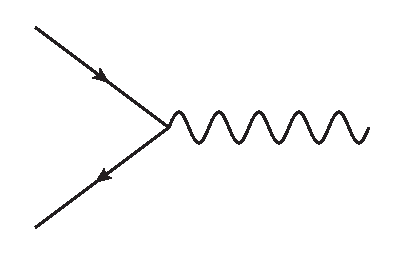
\includegraphics[width=0.6\textwidth]{figures/susyintro/ffg_vertex.eps}
		\caption{ }
		\label{fig:feynmandiagram_supersymmetrization_a}
	\end{subfigure}
	\begin{subfigure}[b]{0.45\textwidth}
		\centering
		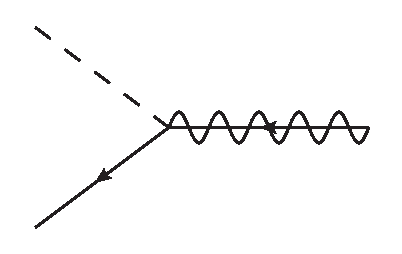
\includegraphics[width=0.6\textwidth]{figures/susyintro/sfg_vertex.eps}
		\caption{ }
		\label{fig:feynmandiagram_supersymmetrization_b}
	\end{subfigure}
	\caption{Feynman diagrams of a {\it fermion-fermion-gauge boson} vertex {\bf (a)} and the supersymmetrized {\it fermion-sfermion-gaugino} vertex {\bf (b)}.}
	\label{fig:feynmandiagram_supersymmetrization}
\end{figure}
An important consequence of the coupling inheritance is that the gaugino fields $\tilde\chi_i^{0/\pm}$ will couple differently depending on the mass mixing matrix. Since the wino field inherits the left-chiral $SU(2)_L$ coupling, the chirality of the couplings of the four neutralinos may differ considerably if the mass eigenstates are close to the gauge eigenstates. In the parameter point used for the analysis in the coming chapters, the second-generation neutralino consists of a large wino part, and this means that it couples weakly to right-chiral quarks. 

 \subsubsection{Sparticle masses}
 The main contributions to the sparticle masses naturally come from the soft terms, since these are responsible for the symmetry breaking which would otherwise give Standard Model masses to sparticles. The mass parameters from these terms are the gaugino mass terms $M_{1,2,3}$, the sfermion mass terms $m_{ij}$ and the Higgs terms $m_{H_{u/d}}$. Additionally, the parameter $\mu$ from the superpotential term coupling the Higgs doublets together in the unbroken SUSY Lagrangian contributes. Now follows a listing of some (s)particle masses, from \cite{Batzing:2013}.
 \begin{itemize}
 	\item At tree level, the different Higgs masses (which have positive R-parity) are
 	\begin{align}
 		m_A^2 &= 2|\mu|^2 + m^2_{H_u} + m^2_{H_d},\nonumber\\
 		m^2_{h,H} &= \frac{1}{2} \left( m_A^2 + m_Z^2 \pm \sqrt{(m_A^2 - m_Z^2)^2 + 4m_Z^2m_A^2\sin^2 2\beta} \right),\\
 		m^2_{H^\pm} &= m_A^2 + m_W^2.\nonumber
 	\end{align}
 	\item The gluino mass $m_{\tilde g}$ is given as
 	\begin{align}
 		m_{\tilde g} = M_3 \left[ 1 + \frac{\alpha_s}{4\pi}\left( 15 + 6\ln\frac{\mu}{M_3} + \sum_{\mathrm{all} \tilde q} A_{\tilde q} \right)\right],
 	\end{align}
 	where $A_{\tilde q}$ are the squark loop contributions given by
 	\begin{align}
 		A_{\tilde q} \int_0^1 dx \, x \ln\left( x \frac{m^2_{\tilde q}}{M_3^2} + (1-x)\frac{m_q^2}{M_e^2} - x(1-x) - i\epsilon \right).
 	\end{align}\marginpar{Not really sure what $M_e$ is...}
 	\item The neutralinos $\tilde\chi_i^0$ are the mass eigenstates of the bino, wino and higgsino fields. In the gauge eigenstate basis, where $\tilde\chi^{0T} = (\tilde B^0, \tilde W^0, \tilde H_d^0, \tilde H_u^0)$, the mass matrix may be written
 	\begin{align}
 		M_{\tilde \chi^0} = \begin{pmatrix}
 			M_1 & 0 & - c_\beta s_{\theta_W} m_Z &  s_\beta s_{\theta_W} m_Z \\
 			0 & M_2 &  c_\beta c_{\theta_W} m_Z & - s_\beta c_{\theta_W} m_Z\\
 			- c_\beta s_{\theta_W} m_Z &  s_\beta s_{\theta_W} m_Z & 0 & -\mu \\
			 c_\beta c_{\theta_W} m_Z & - s_\beta c_{\theta_W} m_Z & -\mu & 0
 		\end{pmatrix},
 	\end{align}
 	where $c_x = \cos x$ and $s_x = \sin x$. For a given parameter choice, this matrix must be diagonalized to find the neutralino masses.
 	\item The charginos $\tilde\chi_i^\pm$ have analogous structure. In the gauge eigenstate basis $\tilde \chi^{\pm T} = (\tilde W^+, \tilde H_u^+, \tilde W^-, \tilde H_d^-)$, the mass matrix is
 	\begin{align}
 		M_{\tilde \chi^\pm} = \begin{pmatrix}
 			0 & 0 & M_2 & \sqrt{2} c_\beta m_W  \\
 			0 & 0 & \sqrt{2} s_\beta m_W & \mu \\
 			M_2 & \sqrt{2} s_\beta m_W & 0 & 0\\
 			\sqrt{2} s_\beta m_W & \mu & 0 & 0
 		\end{pmatrix}.
 	\end{align}
 	\item The first two generations of {\it sfermions}, superpartners of the Standard Model fermions, get masses according to
 	\begin{align}
 		m^2_F = m^2_{F,\mathrm{soft}} + \Delta_F,
 	\end{align}
 	where $m^2_{F,\mathrm{soft}}$ is the mass term from the soft term of the form $-m^2_F F^\dag F$ and $\Delta_F$ is given by
 	\begin{align}
 		\Delta_F = (T_{3F} - Q_F \sin^2\theta_W)\cos 2\beta m^2_Z,
 	\end{align}
 	where $T_{3f}$, $Y$ and $Q$ are the weak isospin, hypercharge and electric charge, respectively, of the left-handed supermultiplet to which the sfermion belongs. The masses are then {\it e.g.}\
 	\begin{align}
 		&m^2_{\tilde e_L} = m^2_{L_1} + \Delta \tilde e_L,\\
 		&m^2_{\tilde e_R} = m^2_{e_R} + \Delta \tilde e_R.
 	\end{align}
 	The mass-splitting between same-generation sleptons and squarks are quark/lepton- and generation-independent and given by {\it e.g.}\ \marginpar{Is it the same for right-handeds? Check, or don't mention?}
 	\begin{align}
 		m^2_{\tilde e_L} - m^2_{\tilde \nu_L} = m^2_{\tilde d_L} - m^2_{\tilde u_L} = -\cos 2\beta m_W^2.
 	\end{align}
 	\item The third-generation sfermions get more complicated masses, given for {\it e.g.}\ the stop squark by the mass matrix (in the chiral gauge eigenstate basis $\tilde t^T = (\tilde t_L, \tilde t_R)$)
 	\begin{align}
 		m^2_{\tilde t} = \begin{pmatrix}
 			m^2_{Q_3} + m_t^2 + \Delta \tilde u_L & v(a_t^* \sin\beta - \mu y_t \cos\beta)\\
 			v(a_t \sin\beta - \mu^* y_t \cos\beta) & m^2_{u3} + m^2_t + \Delta \tilde u_R
 		\end{pmatrix},
 	\end{align}
 	which can be diagonalized to find the mass eigenstates.
 \end{itemize}

 \subsection{Gauge unification and mass hierarchies}
 It was mentioned in the introduction that one very appealing feature of supersymmetry is that the coupling constants of the electromagnetic, weak and strong interactions can be made to unite at a high energy scale. By assuming such a unification at the ``grand unification scale'' $m_\mathrm{GUT} \approx 2\times 10^{16} \,\mathrm{GeV}$, and evolving the SUSY parameters down to the low scale using the $\beta$ functions from the Callan-Symanzik equation, it can be shown that at a scale of 1 TeV, the ratio of the soft mass parameters $M_{1,2,3}$ is
 \begin{align}
 	M_3 : M_2 : M_1 = 6 : 2 : 1.
 \end{align}
 This propagates into the mass formulas to predict the approximate mass relationships
 \begin{align}
 	m_{\tilde g} \approx 6m_{\tilde \chi_1^0}, \, \mathrm{and} \, m_{\tilde \chi_2^0} \approx m_{\tilde \chi_1^\pm} \approx 2m_{\tilde \chi_1^0}.
 \end{align}

\section{The Constrained MSSM}
The available parameter space of the general MSSM is very large, of the order 100 free parameters. It is therefore conventional to make some restricting assumptions. A much-studied restriction is the {\it Constrained MSSM} (CMSSM), also known as {\it minimal supergravity} (mSUGRA). This model is constructed by assuming that SUSY breaking is mediated by some mechanism of gravity at the Planck scale of $M_P = 2.4\times 10^{18} \, \mathrm{GeV}$. By assuming a minimal form for the parameters at the GUT scale, to obtain gauge unification, the resulting model is parametrized in terms of five parameters,
\begin{align}
	m_{1/2}, \, m_{0}, \, A_0, \, \tan\beta \, \mathrm{and} \, \mathrm{sign}(\mu).
\end{align}
The mass parameters $m_{1/2}$ and $m_0$ are the common masses of all gauginos and sfermions, respectively, at the GUT scale. The mass splitting between sparticles appears when the individual sparticle masses are evolved down to a lower scale.
\begin{figure}[hbt]
	\centering
	\includegraphics[width=0.8\textwidth]{figures/susyintro/MSSMrun.eps}
	\caption{MSSM RGE running, from \cite{Martin:1997ns}.}
	\label{fig:mssm_rgerun}
\end{figure}
This is illustrated in fig. \ref{fig:mssm_rgerun} for one choice of $m_{1/2}$ and $m_0$. The figure also illustrates the evolution of $m_{H_u}$ down to a negative value, facilitating the radiative electroweak symmetry breaking.

Because the renormalization running, which is proportional to the mass of the Standard Model partners, the sfermion partners will often get an inverted mass hierarchy compared to the Standard Model. Especially in the colour sector, where stop and sbottom are often the lightest squarks. However, the effect may be compensated by other terms, and often the mass splittings are small.



\section{The experimental status of SUSY}
Include some ATLAS plots. Say something about $B_s \to \mu^+ \mu^-$ at LHCb and constraints on $\tan \beta$? Discuss mSUGRA validity. Mention more general naturalness condition?

\begin{figure}[hbt]
	\centering
	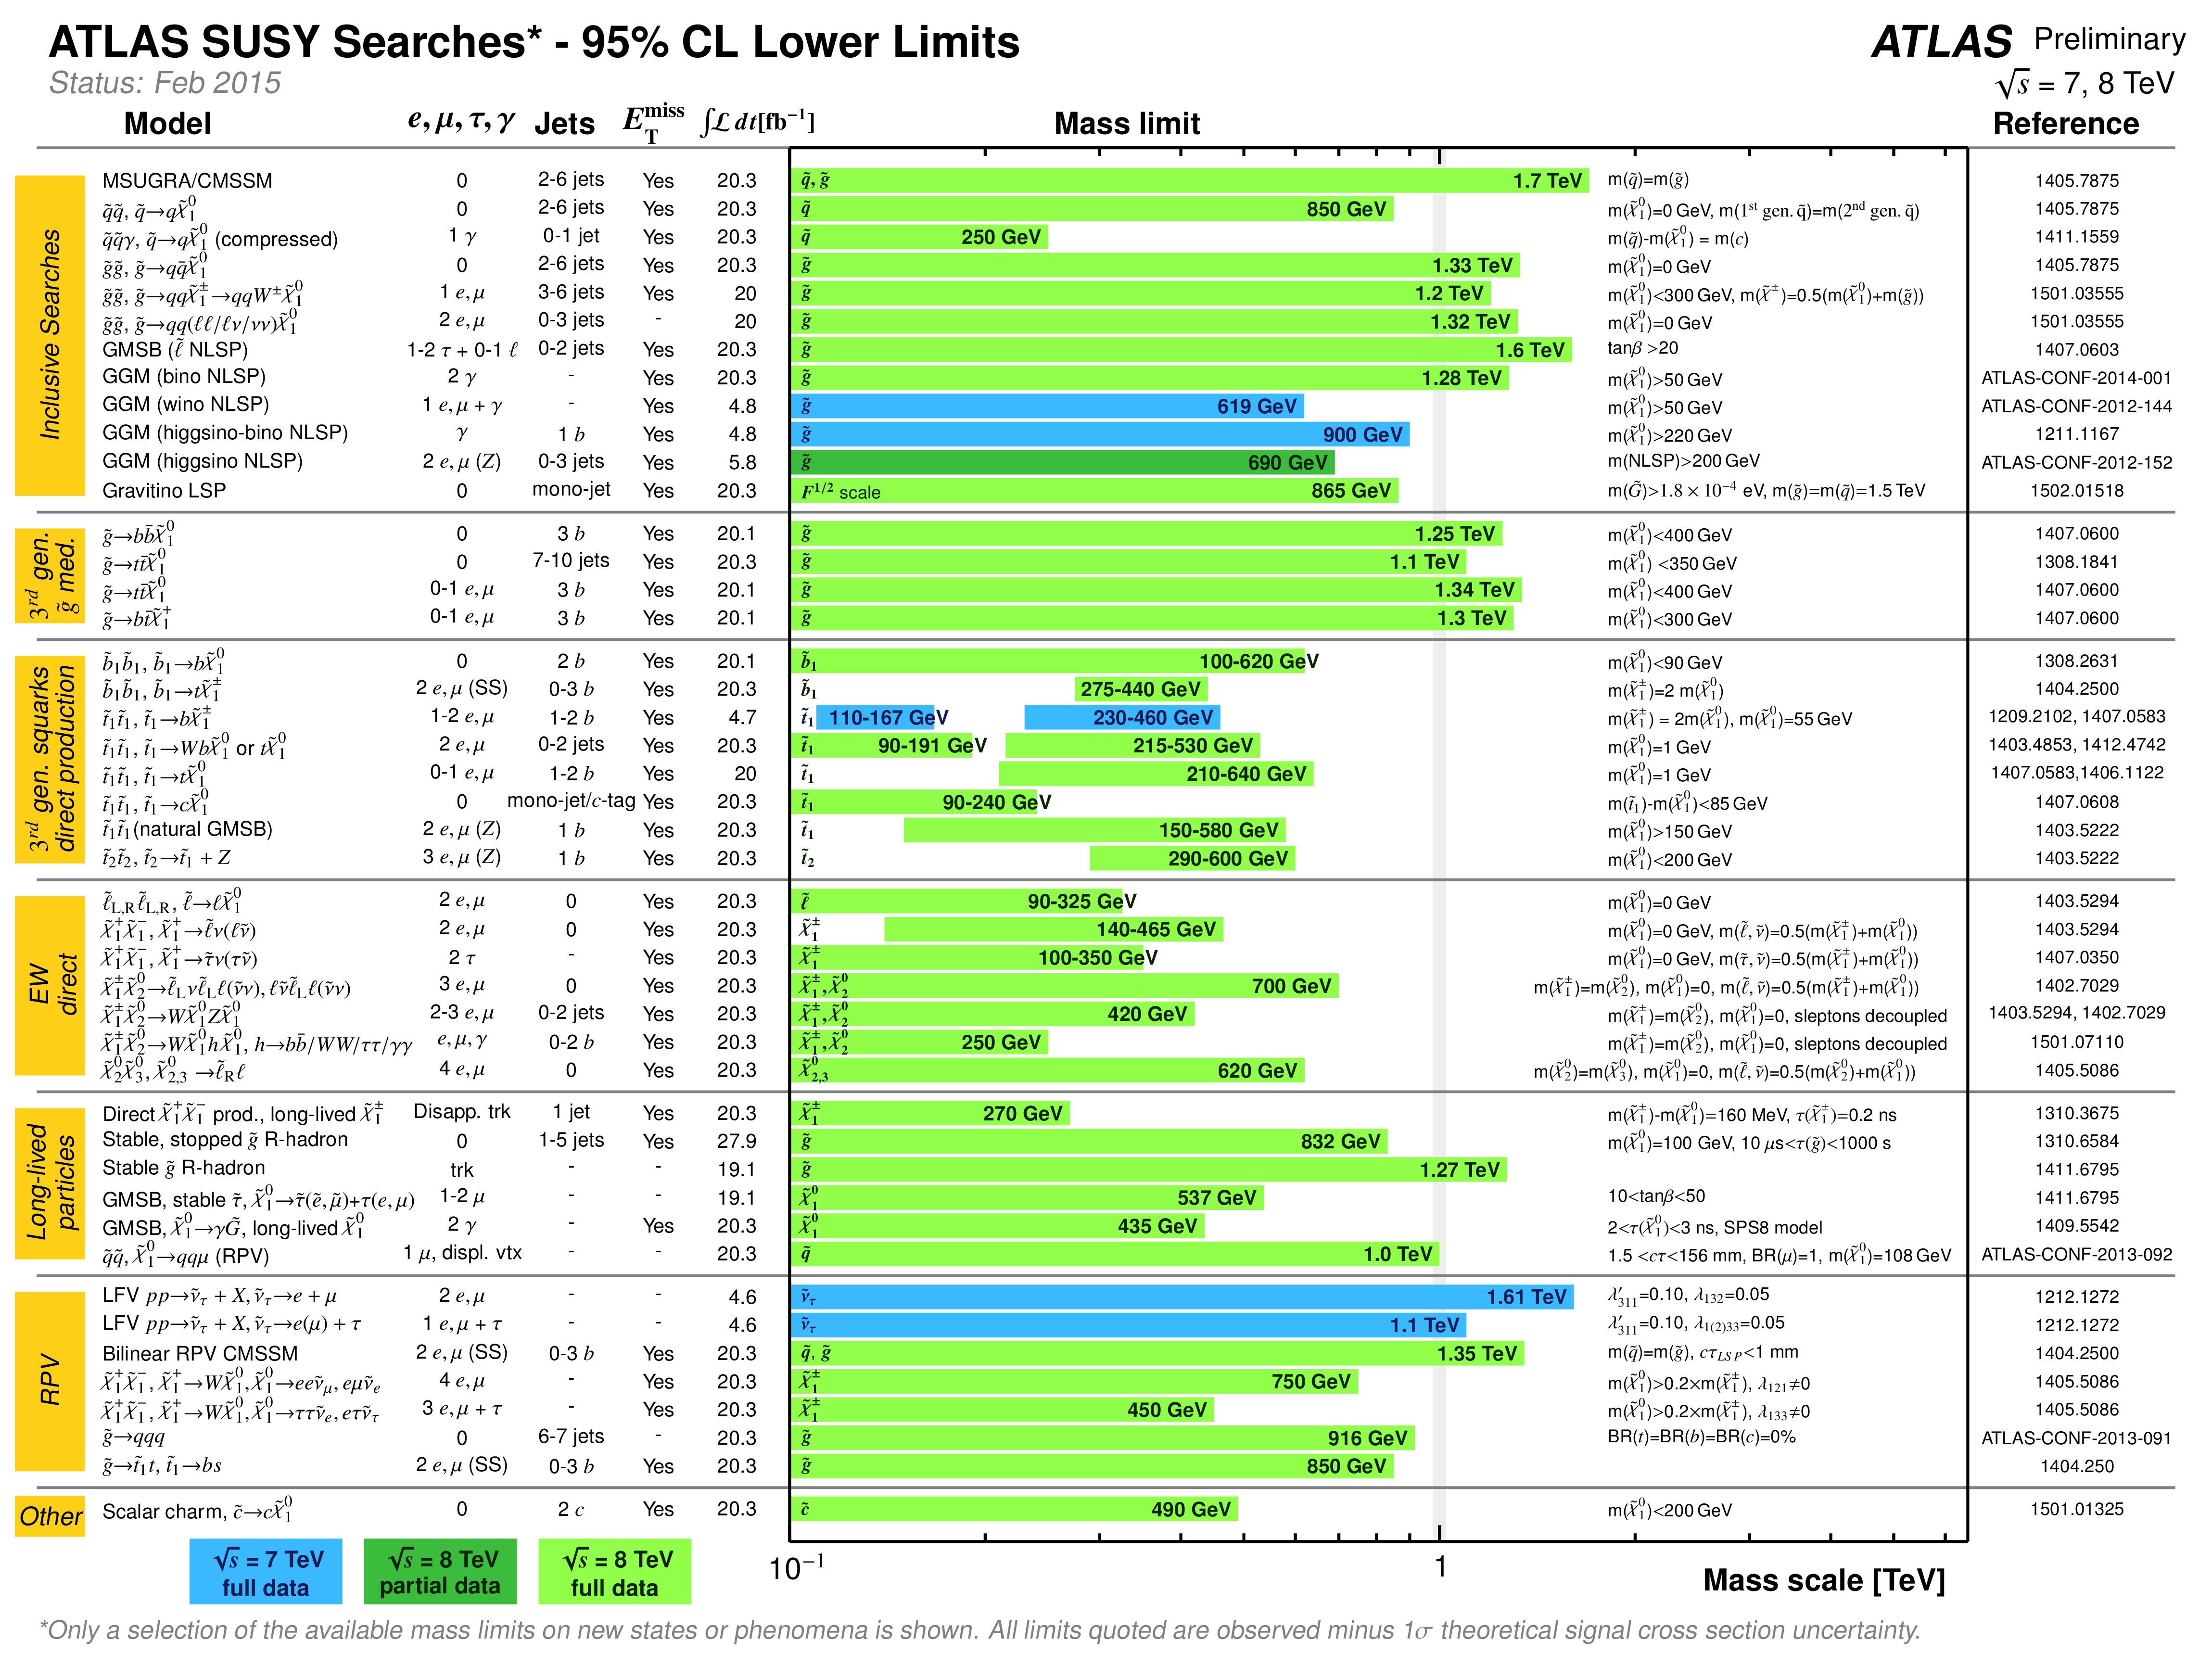
\includegraphics[width=1\textwidth]{figures/susyintro/ATLAS_SUSY_Summary.png}
	\caption{Summary of ATLAS SUSY limits per feb.\ 2015. }
	\label{fig:higgspot}
\end{figure}

\begin{figure}[hbt]
	\centering
	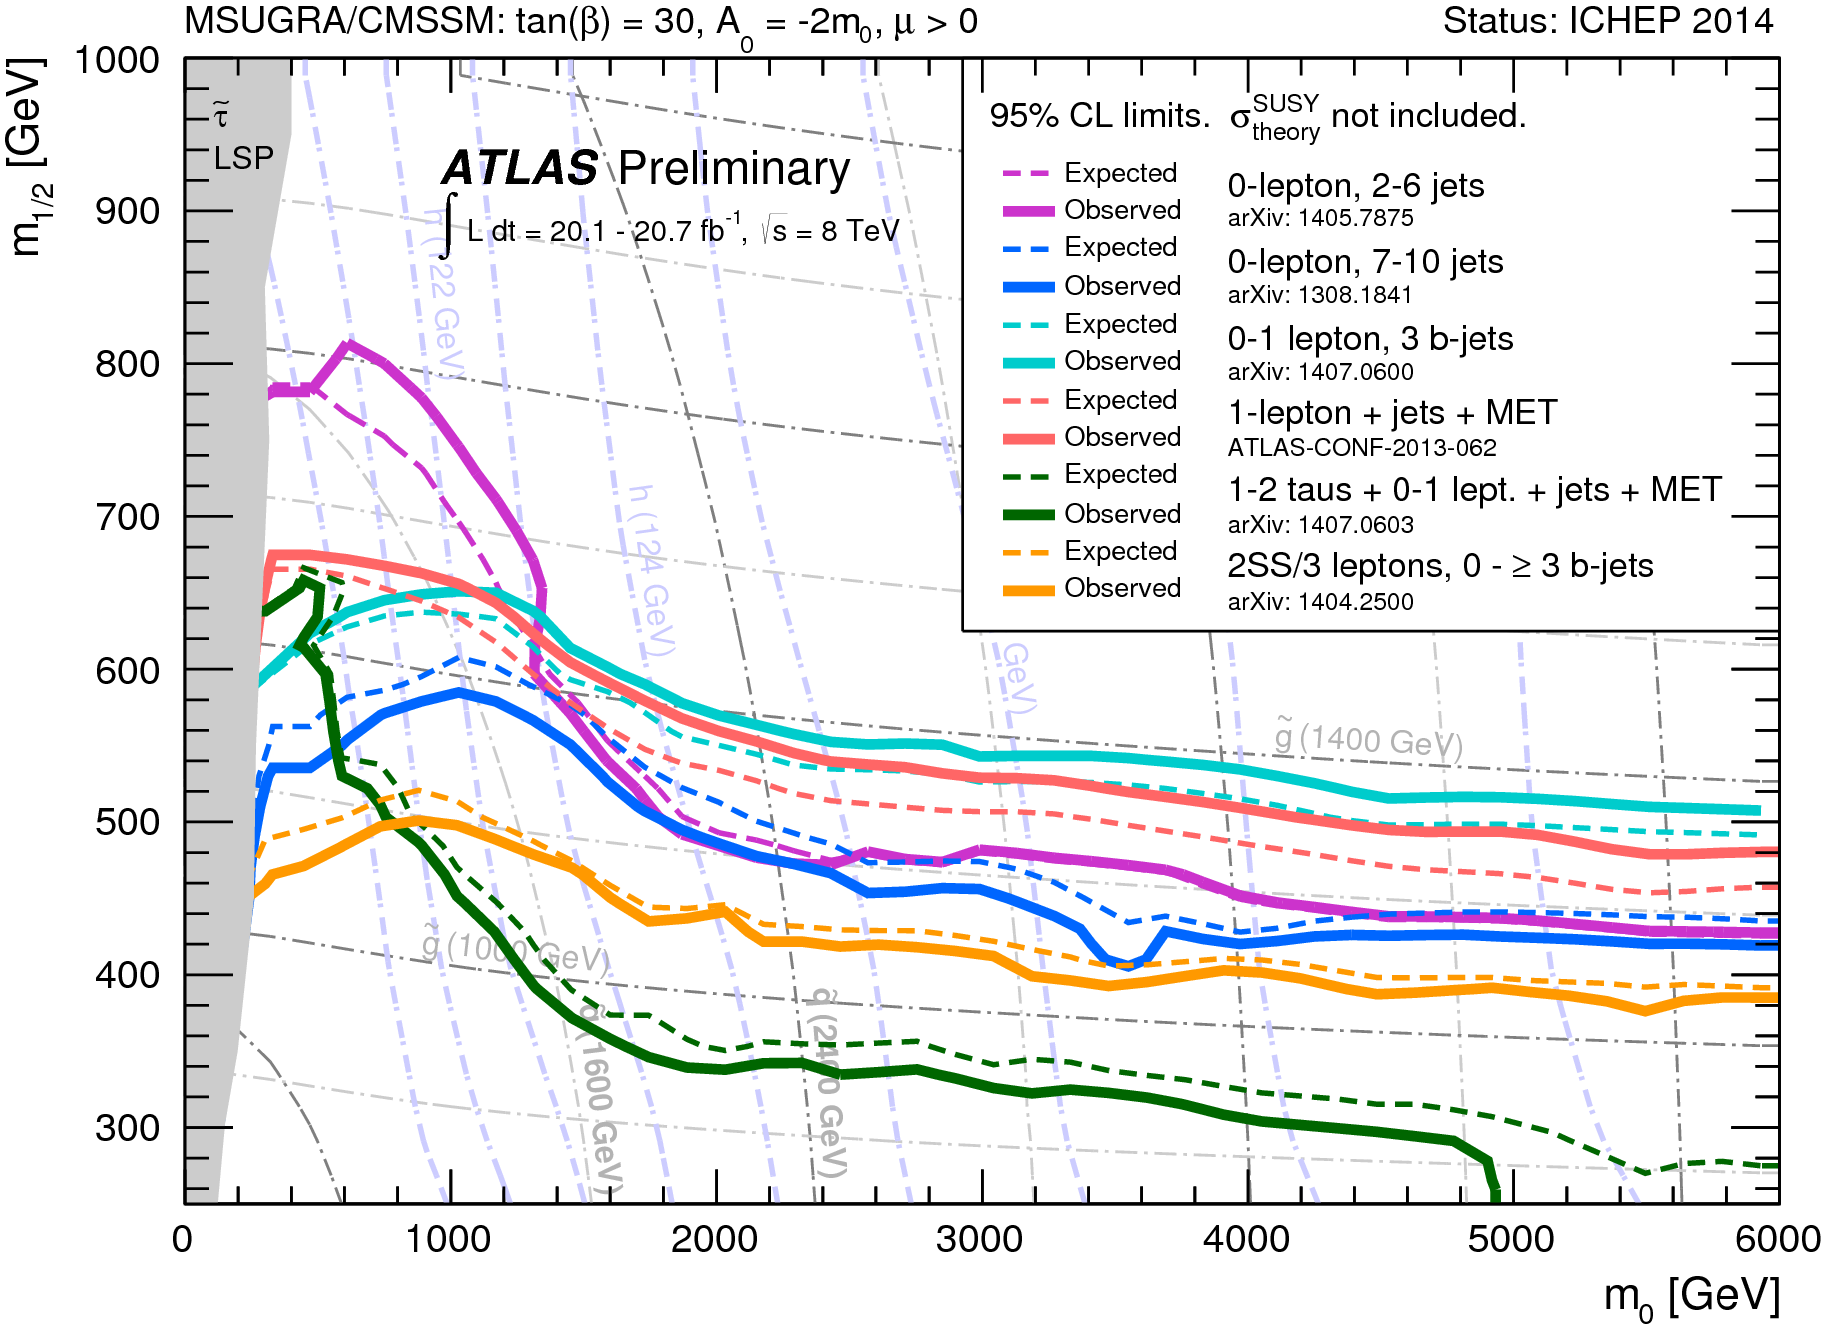
\includegraphics[width=0.9\textwidth]{figures/susyintro/ATLAS_SUSY_MSUGRA.png}
	\caption{mSUGRA/CMSSM limits from ATLAS per feb.\ 2015. }
	\label{fig:higgspot}
\end{figure}
%%%%%%%%%%%%%%%%%%%%%%%%%%%%%%%%%%%%%%%%%%%%%%%%%%%%%%%%%%%
\chapter{The Standard Model of Particle Physics}%%%%%%%%%%%%%%%%%%%%%%%%%%%%%%%%%%%%
%%%%%%%%%%%%%%%%%%%%%%%%%%%%%%%%%%%%%%%%%%%%%%%%%%%%%%%%%%%
\label{ch:SM_intro}
The Standard Model of particle physics has been hugely successful in explaining what our universe consists of at the smallest length scales, and how these constituents interact with each other. It recieved a final, spectacular confirmation in 2012, when a Higgs boson consistent with the predictions of the Standard Model was discovered by the CMS and ATLAS experiments at CERN \cite{Aad:2012tfa, Chatrchyan:2012ufa}. It is well known, however, that the Standard Model is incomplete as a description of our universe, for instance since it gives no explanation for dark matter. There are also more technical problems with the Standard Model, such as the hierarchy problem of the Higgs boson mass loop corrections and the arbitrariness of the model parameters.

The present chapter gives a brief introduction to the principles that underlie the construction of the Standard Model, and outlines the derivation of the model. 
% The presentation is based on \cite{Mandl-Shaw} and \cite{Peskin-Schroeder}.

\section{Symmetries and conservation laws}
Symmetries are manifest in most physical systems. For instance, the special theory of relativity is symmetric under boosts and rotations, as well as translations in space and time. There is a deep relationship between symmetries and the conservation of physical quantities. This result is known as Noether's theorem, and was proven by Emmy Noether in 1915 \cite{Noether:1918zz}. It states that {\it every differentiable symmetry of the action of a physical system has a corresponding conservation law}. In the example of special relativity, the symmetries under translations in time and space correspond to conservation of energy and momentum.%, and the symmetry under rotation corresponds to conservation of angular momentum. \marginpar{What is the conserved quantity under boosts? Is it that ljyubliajsnski polarization vector? Check.}

\subsection{Description by groups}
It is often convenient to describe the symmetries of physical systems in the language of group theory. A group is a set of objects which are closed under some binary operation --- meaning that any combination of two group elements yield another group element. Also, the group must contain an identity element, every element must have an inverse, and the binary operation must be associative. The set of all Lorentz boosts and rotations in special relativity form a group, called the Lorentz group, and together with all spatial translations they form the Poincar\'{e} group. 

The experimental fact that there exist a number of conserved quantities in particle physical systems --- examples include energy and momentum, but also electrical and colour charge, among others --- can be used to construct a theory of particle interactions, by finding the symmetries, and the symmetry groups, that correspond to these quantities and demanding that the theory be symmetric under their action.

An important type of group is the $SU(n)$ group. In the defining representation, this group consists of all complex unitary $n\times n$ matrices of determinant 1. The $SU(n)$ groups are {\it Lie groups}, which means that they are continuous --- {\it i.e.}\ that it is possible to find group elements that are arbitrarily close to the identity. Also, any transformation in the group may be constructed by successive application of such infinitesimal transformations. 

The group elements, and the objects on which the group acts, may be given in several {\it representations}. In the case of matrix groups this means matrices and vectors of different dimension. For an $SU(n)$ group, the two most important representations are the defining, or {\it fundamental}, representation, where the vectors have dimension $n$, and the {\it adjoint} representation, where the vectors have dimension $n^2-1$.

The fundamental definition of a Lie group is given by its corresponding {\it Lie algebra}, which is written\footnote{Here, and in the following, repeated indices are summed over.} 
\begin{align}
	[T_a, T_b] = i f_{abc}T_c.
\end{align}
The objects $T_a$ are called the {\it generators} of the Lie group, and the $f_{abc}$ are called the {\it structure coefficients}. The structure coefficients uniquely determine the group. For $SU(n)$, there are $n^2 - 1$ generators, so $a,b,c =1,...,n^2-1$. For a general Lie group, the binary operation $[\cdot , \cdot ]$, called the {\it Lie bracket}, must be specified, but for $SU(n)$ is is just the commutator
\begin{align}
	[T_a, T_b] = T_aT_b - T_bT_a.
\end{align}

An element $G$ of an $SU(n)$ group may generally be written as
\begin{align}
	G = e^{i\alpha_a O_a},\label{eq:global_gauge_transformation}
\end{align}
in an open neighbourhood of the identity element in $SU(n)$. Here, $O_a = T_a$ in the fundamental representation, and $O_a = (f_{ij})_{a}$ in the adjoint representation. For $SU(2)$, the fundamental representation of the generators are proportional to the Pauli matrices $\sigma_i$, and for $SU(3)$ they are proportional to the Gell-Mann matrices $\lambda_i$. Formally, $G$ is the {\it exponential map} from a Lie algebra to its corresponding Lie group. 

The exponential map may be extended from a {\it global} transformation to a {\it local} transformation with respect to some underlying manifold $X$ by letting $\alpha_a = \alpha_a(x)$, where $x\in X$. For the purposes of the Standard Model, $X$ is space-time.




\section{Ingredients of the Standard Model}

The Standard Model consists of 12 fermions with corresponding antifermions, a number of vector gauge bosons and one scalar boson, whose existence have all been verified experimentally. The gauge bosons mediate interactions between the particles. There are three fundamental interactions in the Standard Model: The electromagnetic interaction, the weak interaction and the strong interaction. The combination of electromagnetic and weak interactions are often referred to as the {\it electroweak} theory, while the theory describing the strong interaction is known as {\it Quantum Chromonynamics (QCD)}. Note that not all particles couple to each other with all of the interactions. 

The fermions are divided into two groups, the quarks and leptons. There are six different {\it flavours} of quarks, called up, down, strange, charm, bottom and top, in order of increasing mass. They are subdivided into three generations of pairs, up/down, charm/strange and top/bottom. The up, charm and top quarks carry quanta of $+\frac{2}{3}$ of the fundamental electrical charge $e$, while the down, strange and bottom quarks carry $-\frac{1}{3}e$. There are also six leptons, of which three are charged. They are called the electron, the muon and the tau. They each belong in a generation of their own, together with their neutral counterparts, the electron neutrino, muon neutrino and tau neutrino, respectively. 

The vector gauge bosons consist of the photon, the $Z$ and $W$ bosons and the gluon. The photon is the mediator of electromagnetic interactions, the $Z$ and $W$ mediate the weak interaction and the gluon mediates the strong interaction. The photon, $Z$ boson and gluon are all neutral, and they are their own antiparticles. The photon and gluon are massless, while the $W$ and $Z$ bosons are quite heavy. The $W$ carries one elementary unit of electric charge, and is thus distinct from its antiparticle, with a difference in sign for the particle and antiparticle states. The scalar boson of the Standard Model is the Higgs boson, which is responsible for giving particles their observed mass through the Higgs mechanism. It is electrically neutral and very massive.

Among the fermions, only the quarks couple to the strong interaction. All the known fermions couple with the weak interaction, while only the electrically charged fermions couple electromagnetically --- {\it i.e.}\ all except the neutrinos. They couple to the Higgs field proportionally to their mass, so that for instance the top quark, which is the heaviest Standard Model particle, couples the strongest. A schematic overview of the particles in the Standard Model is shown in fig.\ \ref{fig:SM_particles}.
\begin{figure}[hbt]
	\centering
	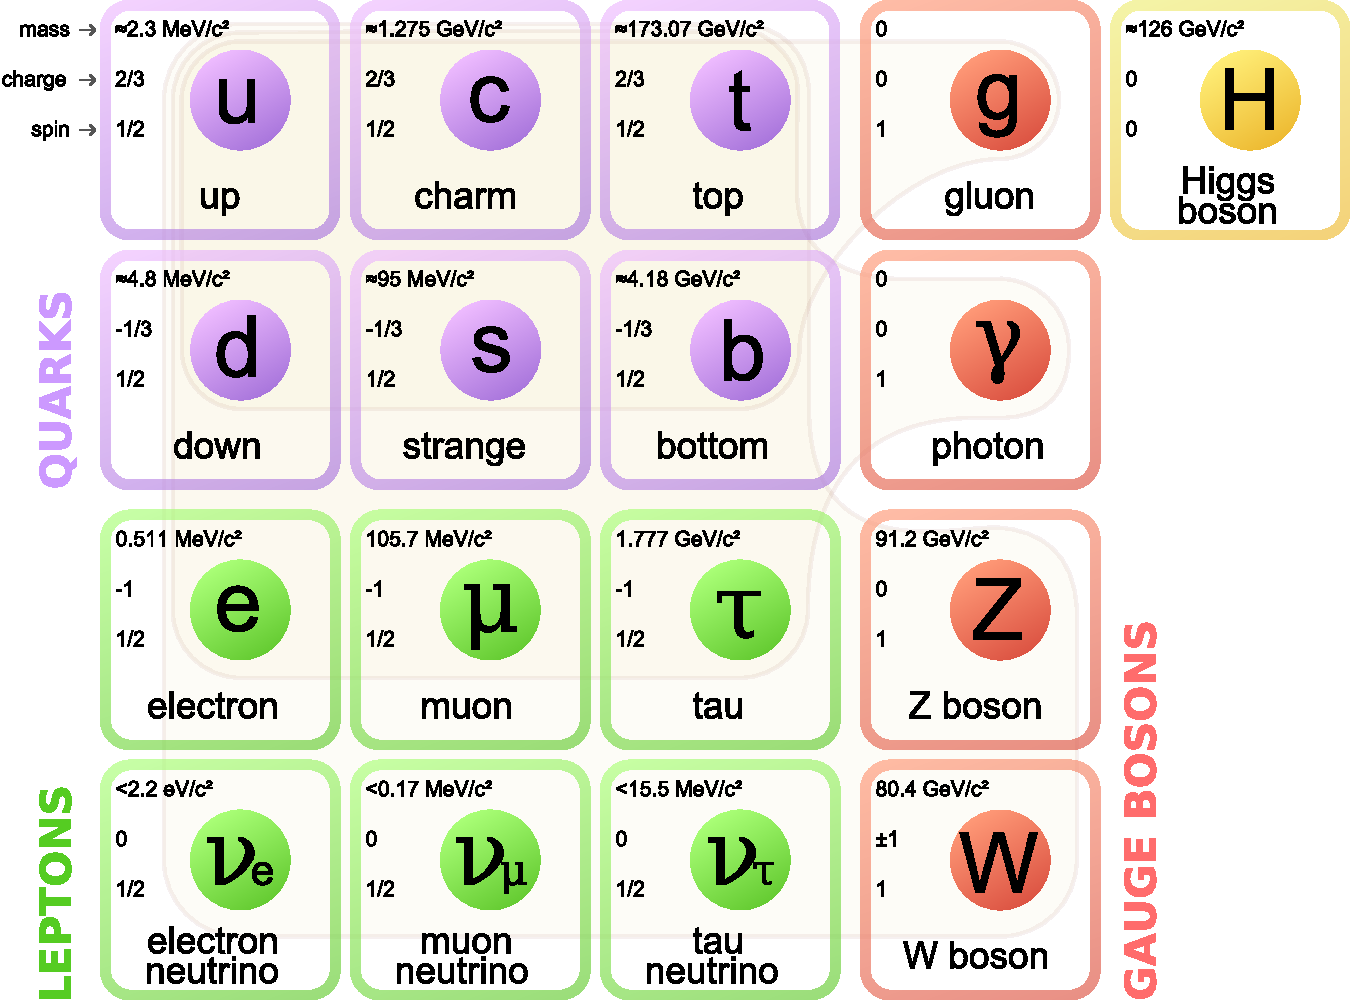
\includegraphics[width=0.8\textwidth]{figures/susyintro/Standard_Model_of_Elementary_Particles.pdf}
	\caption{An overview of the particles of the Standard Model and their interactions, from \cite{Wikimedia_SM_particles}.}
	\label{fig:SM_particles}
\end{figure}

The flavours of the quarks and leptons are conserved in the electromagnetic and strong interactions. For instance, a top quark cannot change into a charm or up quark by emission of a photon or gluon. The weak interaction enables the top quark to change into a bottom quark, or a tau lepton to change into a tau neutrino, through the emission of a charged $W$ boson. This would still seem to conserve the {\it generation} of quark or lepton, but breaking of generation is also made possible through the mechanism of {\it generation mixing}, quantified by the Cabibbo-Kobayashi-Maskawa (CKM) matrix for the case of quarks and the Pontecorvo-Maki-Nakagawa-Sakata (PMNS) matrix for the leptons. The PMNS mixing also explains the observed phenomenon of {\it neutrino oscillations} (if the neutrinos are assumed to be massive, which they are technically not in the Standard Model).

\section{Constructing the Lagrangian of the Standard Model}

The Standard Model is a quantum field theoretic model, and may be stated in terms of a Lagrangian density function $\mathcal{L}$. The guiding principle for constructing the Lagrangian is {\it gauge invariance}. Gauge degrees of freedom are physical degrees of freedom which are ``superflous'', in the sense that they do not have any observable consequences. An example is Maxwell's theory of electromagnetism, where the electromagnetic vector potential $A^\mu$ is undetermined up to the addition of a total derivative term $\partial^\mu \phi$. The gauge freedom is exploited by requiring that the Lagrangian, which determines the physical dynamics, does not change when the gauge degrees of freedom are varied, {\it i.e.}\ that it is gauge invariant. This invariance is related to conservation of physical quantities by Noether's theorem.

The Standard Model is based on gauge invariance under three Lie groups, the famous $U(1)_Y\times SU(2)_L\times SU(3)_C$. The different particle types transform in different representations of the groups. In the Standard Model, the fermions transform in the fundamental representation, while the gauge bosons transform in the adjoint representation.

\section{Constructing a gauge theory}
The particle content of the Standard Model is input into the Lagrangian by inserting fermionic fields, {\it i.e.}\ Dirac spinor fields, and imposing the desired gauge invariance on these fields. The basic Dirac term, called the Dirac bilinear, for some spinor field $\psi$, is\footnote{We will, for what follows, set $\hbar = c = 1$.} 
\begin{align}
	\bar \psi (i\gamma^\mu \partial_\mu - m) \psi = \bar \psi (i\slashed\partial - m)\psi, \label{eq:diracbilinear}
\end{align}
where $\gamma_\mu$ are the Dirac matrices, $m$ is the mass of the spinor field, and $\bar\psi \equiv \psi^\dag \gamma_0$. The Dirac bilinear results in the Dirac equation for the field when the equations of motion are applied. The Dirac equation and the Dirac matrices are derived in appendix \ref{appendix:diraceq}.

Next, we impose gauge invariance. The group transformation of an $SU(n)$ group may be written in the fundamental representation as
\begin{align}
	G(x) = e^{ig\alpha_a(x)T_a},\label{eq:gauge_transformation}
\end{align}
where $\alpha(x)$ are $n$ arbitrary real differentiable functions and $T_a$ are the generators of $SU(n)$ in the fundamental representation. We assume that the Lagrangian consists of $n$ Dirac bilinear terms with fields $\psi_i$, and that they are put into an $n$-dimensional multiplet $\Psi = (\psi_1, \psi_2, ..., \psi_n)^T$ such that the basic Dirac Lagrangian reads
\begin{align}
	\mathcal{L}_0 = \bar\Psi(i\slashed\partial - m)\Psi,
\end{align}
where we assume that all fields have the same mass $m$.\footnote{This assumption is often wrong in the case of the Standard Model, but finds its solution in the Higgs mechanism.} The group transformations of the multiplet and its adjoint are then 
\begin{align}
	\Psi(x) &\overset{G}{\to} e^{ig\alpha_a(x)T_a} \Psi(x),\\
	\bar\Psi(x) &\overset{G}{\to} \bar\Psi(x) e^{-ig\alpha_a(x)T_a}.\nonumber
\end{align}
If we apply these transformations to the basic Lagrangian, it becomes
\begin{align}
	\mathcal{L}_0 = &\bar\Psi(x)(i\slashed\partial - m)\Psi(x)\nonumber\\
	\overset{G}{\to} &\bar\Psi(x) e^{-ig\alpha_a(x)T_a}(i\slashed\partial - m)e^{ig\alpha_a(x)T_a} \Psi(x)\\
	=	&\bar\Psi(x)(i\slashed\partial - m)\Psi(x) - g\bar\Psi(x) T_a\slashed\partial \alpha_a(x) \Psi(x).\nonumber
\end{align}
Thus, the basic Dirac Lagrangian is not gauge invariant, since we have picked up an additional term. Gauge invariance may be achieved by adding a term of the form 
\begin{align}
	-\bar\Psi(x) ig\gamma^\mu \alpha_a(x)A_{a,\mu}(x) \Psi(x),\label{eq:covariantderivativeterm}
\end{align}
to the Lagrangian, where $A_{a,\mu}(x)$ is some new field, which we require to transform under $G$ as
\begin{align}
	A_{a,\mu}(x) \overset{G}{\to} A_{a,\mu}(x) + \partial_\mu \alpha_a(x).
\end{align}
If we apply $G$ to the sum of the Dirac bilinear with this new term, it is invariant:
\begin{align}
	&\bar\Psi(x)(i\slashed\partial - m)\Psi(x) - \bar\Psi(x) ig\gamma^\mu \alpha_a(x)A_{a,\mu}(x) \Psi(x)\nonumber\\
	\overset{G}{\to} &\bar\Psi(x)(i\slashed\partial - m)\Psi(x) - g\bar\Psi(x) T_a\slashed\partial \alpha_a(x) \Psi(x)\\
	 &- \bar\Psi(x) ig\gamma^\mu \alpha_a(x)A_{a,\mu}(x) \Psi(x) +  g\bar\Psi(x) T_a\slashed\partial \alpha_a(x) \Psi(x)\nonumber\\
	 = &\bar\Psi(x)(i\slashed\partial - m)\Psi(x) - \bar\Psi(x) ig\gamma^\mu \alpha_a(x)A_{a,\mu}(x) \Psi(x).\nonumber
\end{align}
The term from eq.\ \eqref{eq:covariantderivativeterm} is usually included by replacing $\partial_\mu$ with the {\it covariant derivative}
\begin{align}
	D_\mu = \partial_\mu + igT_a A_{a,\mu}.
\end{align}
The fields $A_{a,\mu}$ are called gauge boson fields, and are responsible for mediating interactions between the Dirac fermion fields. The gauge boson fields must also have their own free-field term in the Lagrangian, called the field strength, which is given from the Proca Lagrangian for spin-1 fields as 
\begin{align}
	-\frac{1}{4} F_{a,\mu\nu} F_a^{\mu\nu},\label{eq:field_strength}
\end{align}
where we can define
\begin{align}
	igT_a F_{a}^{\mu\nu} &\equiv [D_a^\mu, D_a^\nu] \\
	&= igT_a \left[ \partial^\mu A_a^\nu - \partial^\nu A_a^\mu + g f_{abc} A_b^{\mu}(x)A_c^{\nu}(x) \right],
\end{align}
where, again, $f_{abc}$ are the structure coefficients of $SU(n)$. Note that with this definition, the field strength \eqref{eq:field_strength} is gauge invariant.

With this, the total gauge invariant Lagrangian consists of $n$ fermion fields and $n^2-1$ gauge boson fields, and reads
\begin{align}
	\mathcal{L} = \bar\Psi(i\slashed D - m)\Psi - \frac{1}{4} F_{a,\mu\nu} F_a^{\mu\nu}.
\end{align}
The covariant derivative gives rise to terms coupling the fermion and gauge fields together. In the case of $n=1$, the gauge group is the $U(1)$ group, which describes the theory of quantum electrodynamics, the simplest gauge theory. For $U(1)$, the structure coefficients vanish, since there is only a single gauge field,\footnote{This contradicts the claim that there are $n^2-1$ gauge fields --- for $U(n)$ there are $n^2$ of them. The reason is that $U(1)$ is not an $SU(n)$ group, but the above derivation works for $U(1)$ as well.} making the Lagrangian particularily simple. In QED, there are no gauge boson self-interactions. For $n>1$, the structure coefficients do not vanish, and this gives rise to cross terms in the field strength term $-\frac{1}{4} F_{a,\mu\nu} F_a^{\mu\nu}$ coupling the gauge bosons among themselves. These couplings are of great importance in the theories of the weak and strong interactions.




\section{Singlets, doublets and triplets}

As mentioned previously, not all the fields are subject to all the different interactions. If a field couples through a certain interaction, it is said to be {\it charged} under the transformations corresponding to that interaction. A specific amount $g$ of charge is assigned to every field, and enters into the group transformations as in eq.\ \eqref{eq:gauge_transformation}. Thus, for $g=0$, the transformation is the identity and has no effect. In the electromagnetic $U(1)$ case, this charge is the electrical charge, $g=q$. Analogous charges are associated with the $U(1)_Y$, $SU(2)_L$ and $SU(3)_C$ groups. They are called hypercharge, weak isospin and colour charge, respectively. These charges are the conserved quantitites associated with the gauge symmetries, as implied by Noether's theorem.

In the case of $SU(2)$ and $SU(3)$, the fields have to be put into vectors in order to be acted upon by the transformations, as was done in the previous section. Since the fermionic fields transform in the fundamental representation, the dimensions of the vectors are 2 and 3, respectively. These types of vectors are referred to as $SU(2)$ {\it doublets} and $SU(3)$ {\it triplets}.

A Dirac field can be written as the sum of a left-chiral and a right-chiral part, defined by the projection operators 
\begin{align}
	P_{R/L} = \frac{1}{2}\left( 1\pm \gamma^5 \right),
\end{align}
where $\gamma^5 \equiv i\gamma^0\gamma^1\gamma^2\gamma^3$. Given a Dirac field $\psi$, we may write
\begin{align}
	\psi = P_R \psi + P_L \psi \equiv \psi_R + \psi_L.
\end{align}
In the case of $SU(2)_L$, only the left chiral part of the fields are charged under the symmetry. For instance, the left-chiral parts of the quark fields are put in doublets, {\it e.g.}\
\begin{align}
	q_L = \begin{pmatrix}
		u_L \\ d_L
	\end{pmatrix},
\end{align}
for the up- and down-quarks, while the right-handed parts are put in two separate singlets $u_R$ and $d_R$, upon which the $SU(2)_L$ transformation has no effect. This has the consequence that the $SU(2)_L$ interaction is left-chiral --- it only couples to left-handed parts of fields. Due to the spontaneous symmetry breaking of the $U(1)_Y\times SU(2)_L$ symmetry, the chirality is not exact in the resulting weak interactions, but it is still an important feature of the Standard Model.

The $SU(3)_C$ symmetry is the symmetry of the strong force, and among the fermions, only the quarks are charged under it. The quarks transform under $SU(3)$ in triplets --- one for each quark flavour --- where the components of the triplet are discriminated by differing {\it colour}, denoted red, green or blue. 


While the fermions transform under the groups in the fundamental representation, which has dimension $n$ for $SU(n)$, the gauge vector boson fields transform in the adjoint representation, which has dimension $n^2-1$. This number then determines the number of different gauge bosons for each group: $U(1)_Y$ has a single gauge boson field labeled $B^\mu$; $SU(2)_L$ has three, labeled $W^\mu_{1,2,3}$; and $SU(3)_C$ has eight different gauge boson fields, labeled $A^\mu_a$ for $a = 1,...,8$. The $SU(3)_C$ bosons are called {\it gluons}. The $U(1)_Y$ and $SU(2)_L$ bosons are not the ones that we observe --- the physical gauge boson eigenstates are linear combinations of them, mixed together by the spontaneous symmetry breaking of the Higgs mechanism.

\section{The Higgs mechanism}
Gauge invariance forbids the inclusion of terms of the form $m^2A^\mu A_\mu$ into the Lagrangian, which are required in order to give vector bosons such as the $Z$ their observed mass. To include the terms, we must also include a new complex scalar field doublet $\Phi = (\phi_a, \phi_b)^T$. This mechanism was first suggested by Anderson \cite{1963PhRv..130..439A}, and subsequently generalized to a relativistic field theory independently by three groups: Guralnik, Hagen and Kibble \cite{1964PhRvL..13..585G}; Brout and Englert \cite{1964PhRvL..13..321E}; and Higgs \cite{Higgs:1964pj}. It is commonly referred to as the Higgs mechanism. The mechanism introduces the following terms into the Lagrangian:
\begin{align}
	\mathcal L \ni |D_\mu \Phi(x)|^2 - \mu^2|\Phi(x)|^2 - \lambda |\Phi(x)|^4.\label{eq:higgs_lagrange}
\end{align}
The last two terms comprise the Higgs {\it potential}. If $\mu^2$ is assumed to be negative and $\lambda$ positive, then the potential assumes the shape of a ``mexican hat'' as a function of $|\Phi|$. This is shown in fig.\ \ref{fig:higgspot}.
\begin{figure}[hbt]
	\centering
	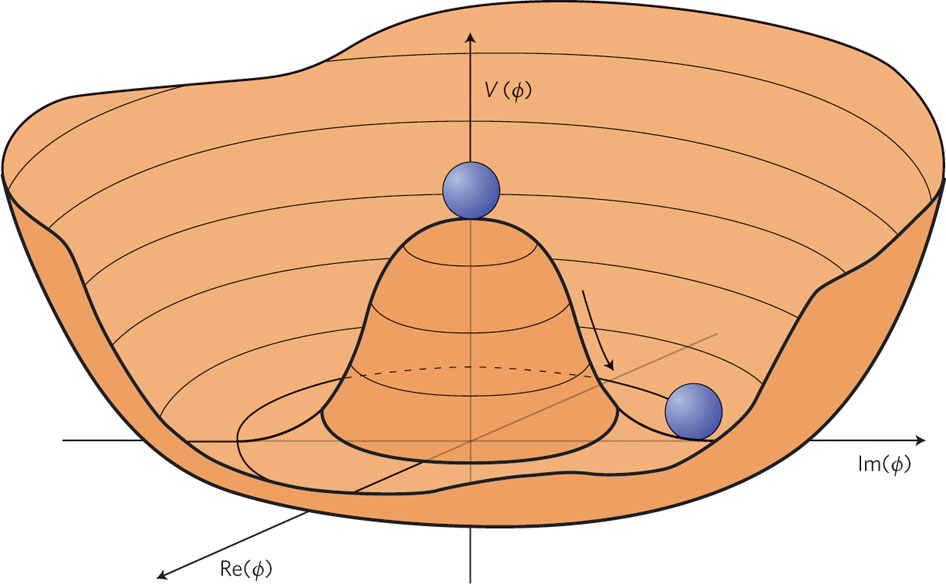
\includegraphics[width=0.5\textwidth]{figures/susyintro/higgspot_nature.jpg}
	\caption{The shape of the Higgs potential, from \cite{Ellis:higgs}.}
	\label{fig:higgspot}
\end{figure}
This potential has a circle of degenerate energy at the field value $|\Phi_0|^2 = |\phi_a^0|^2 + |\phi_b^0|^2 = -\mu^2/2\lambda$. The mechanism of {\it spontaneous symmetry breaking} occurs when, as the energy decreases, the Higgs field falls to the bottom of the degenerate circle and is forced to {\it choose} a particular point on the circle for its lowest energy state, the vacuum. This causes $\Phi$ to obtain a {\it vacuum expectation value} (vev) $\langle \Phi_0 \rangle = (-\mu^2/\lambda)^{1/2} \equiv v$. Without loss of generality, we may write $\Phi_0$ as
\begin{align}
	\Phi_0 = \frac{1}{\sqrt{2}} \begin{pmatrix}
		0 \\ v
	\end{pmatrix}
\end{align}
in the vacuum state. For a general energy state, $\Phi$ can be written
\begin{align}
	\Phi = \frac{1}{\sqrt{2}} \begin{pmatrix}
		\eta_1(x) + i\eta_2(x) \\
		v + H(x) + i\eta_3(x)
	\end{pmatrix}.
\end{align}
One can find parameters $\xi_j$ such that, for a gauge transformation $G \in U(1)_Y\times SU(2)_L$, if
\begin{align}
	G^{-1} = e^{\frac{i}{v}\left(\xi_j\frac{1}{2}\sigma_j\right)} e^{\frac{i}{v} \xi_3},
\end{align}
then
\begin{align}
	\Phi = \frac{1}{\sqrt{2}} G^{-1} \begin{pmatrix}
		0 \\ v + H(x)
	\end{pmatrix}.
\end{align}
Then, by gauge transforming the Lagrangian $\mathcal{L}$ using $G$, one obtains
\begin{align}
	\Phi \overset{G}{\to} \Phi' = \frac{1}{\sqrt{2}}\begin{pmatrix}
		0 \\ v + H(x)
	\end{pmatrix},
\end{align}
and simultaneously, the vector gauge fields transform as
\begin{align}
	W^\mu_i &\overset{G}{\to} W'^\mu_i ,\label{eq:SSB_gauge_transformation}\\
	B^\mu &\overset{G}{\to} B'^\mu .\nonumber
\end{align}
In this gauge, the three degrees of freedom represented by the real scalar fields $\eta_i(x)$ are not present. The interpretation is that they are absorbed into the three bosons $W^\pm$ and $Z$, providing the longitudinal polarization degrees of freedom required for massive vector bosons. The remaining real scalar field $H(x)$ is the Higgs field.

This gauge choice also makes apparent that the gauge fields $W^\mu_i$ and $B^\mu$ mix together into the physical mass eigenstates $W^{\pm\mu}$ and $Z^\mu$. This can be seen from the covariant derivative term in eq.\ \eqref{eq:higgs_lagrange}. In this gauge, the covariant derivative of $\Phi$ is
\begin{align}
	D'^\mu \Phi' = \left[ \partial^\mu + i g \frac{\sigma_j}{2} W_j'^\mu + i \frac{1}{2} g' B'^\mu \right]\frac{1}{\sqrt{2}}\begin{pmatrix}
		0 \\ v + H(x)
	\end{pmatrix},
\end{align}
where $g$ and $g'$ are the coupling constants of $SU(2)_L$ and $U(1)_Y$, respectively, and $\sigma_j$ are the Pauli matrices. By multiplying out, this becomes
\begin{align}
	\begin{pmatrix}
		\frac{ig}{2}(W'^\mu_1 - iW'^\mu_2) \frac{v+H(x)}{\sqrt{2}} \\
		\left( \partial^\mu - \frac{ig}{2}W'^\mu_3 + \frac{ig'}{2} B'^\mu \right) \frac{v+H(x)}{\sqrt{2}}\nonumber \label{eq:higgs_covariant_derivative_gauge_eigenstates}
	\end{pmatrix}.
\end{align}
By defining 
\begin{align}
	\tan\theta_W &= \frac{g'}{g},\nonumber\\
	{W'}^\mu_3 &= \cos\theta_W Z^\mu + \sin\theta_W A^\mu,\\
	{B'}^\mu &= -\sin\theta_W Z^\mu + \cos\theta_W A^\mu,\nonumber\\
	W^{\pm \mu} &= \frac{1}{\sqrt{2}} \left({W'}_1^\mu \mp i{W'}_2^\mu \right),\nonumber
\end{align}
where $\theta_W$ is called the {\it Weinberg angle}, eq.\ \eqref{eq:higgs_covariant_derivative_gauge_eigenstates} becomes 
\begin{align}
	D'^\mu\Phi' = \frac{1}{\sqrt{2}} \begin{pmatrix}
		\frac{ig}{\sqrt{2}} W^{+\mu}\left(v+H(x)\right) \\
		\partial^\mu H(x) - \frac{ig}{2\cos\theta_W}Z^\mu \left(v+H(x)\right) 
	\end{pmatrix}.
\end{align}
Thus, the kinetic term $|D^\mu \Phi|^2$ is
\begin{align}
	|D^\mu \Phi|^2 = \frac{1}{2}&\left( \frac{g^2v^2}{2} W^{+\mu} W^-_\mu + g^2vHW^{+\mu}W^-_\mu \right.\nonumber\\
	&+ \frac{g^2}{2} W^{+\mu}W^-_\mu H^2 + \partial^\mu H \partial_\mu H + \frac{g^2v^2}{4\cos^2\theta_W} Z^\mu Z_\mu \\
	&+ \left. \frac{g^2}{2\cos^2\theta_W} v Z^\mu Z_\mu H + \frac{g^2}{4\cos^2\theta_W}Z^\mu Z_\mu H^2 \right).\nonumber
\end{align}
This expression contains mass terms for the $Z$ and $W^\pm$ bosons, fixing their masses to
\begin{align}
	m_Z = \frac{1}{2\cos\theta_W}vg, \quad m_W = \frac{1}{2}vg.
\end{align}
Note that this means that
\begin{align}
	m_Z = \frac{m_W}{\cos\theta_W}.
\end{align}
Note also that there is no mass term for the photon field $A^\mu$ --- it remains massless after symmetry breaking. This allows for the remaining $U(1)_\mathrm{em}$ symmetry, where $A^\mu$ is the corresponding gauge boson and the gauge charge is the electrical charge, which by Noether's theorem must be conserved in all processes of the Standard Model.

The Higgs mechanism also provides fermionic terms of the form 
\begin{align}
 	\bar\psi_i \psi_j y_{ij}(v+H) = y_{ij} \bar \psi_i  \psi_j H + v y_{ij} \bar\psi_i \psi_j.
 \end{align} 
 The terms of the first type couple the fermions to the Higgs field. For $i=j$, the terms of the second type are mass terms of the form written in the Dirac bilinear, eq.\ \eqref{eq:diracbilinear}, and for $i\neq j$ they give rise to off-diagonal terms in the CKM and PMNS matrices. The coupling constants of these terms are called {\it Yukawa couplings}.

\section{The Feynman calculus and loop corrections}
\label{subsec:feynmancalculus}
Very few problems in the framework of the Standard Model can be solved exactly. Instead, calculations are done using perturbation theory to series expand the solution as an infinite sum of increasingly complicated, but decreasingly important, contributions in terms of powers of some small parameter. Feynman invented a technique for visualizing these expansions using diagrams, known as Feynman diagrams \cite{2005AmericanScientist}. For instance, the problem of inelastic electron-positron scattering has as one of its leading contributions the diagram shown in fig.\ \ref{fig:feynmandiagram_a}. The next-to-leading order in the fine-structure constant $\alpha = e^2/4\pi$ includes the diagrams in figs. \ref{fig:feynmandiagram} (b), (c) and (d).
\begin{figure}[htbp]
	\centering
	\begin{subfigure}[b]{0.45\textwidth}
		\centering
		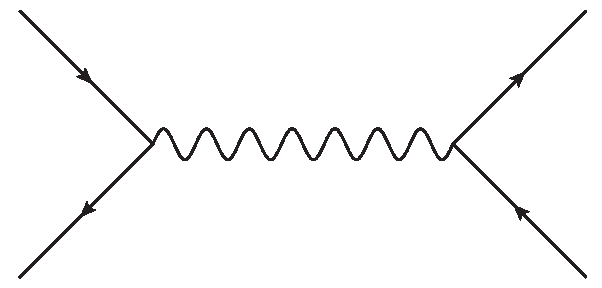
\includegraphics[width=0.6\textwidth]{figures/susyintro/epscattering.pdf}
		\caption{ }
		\label{fig:feynmandiagram_a}
	\end{subfigure}
	\begin{subfigure}[b]{0.45\textwidth}
		\centering
		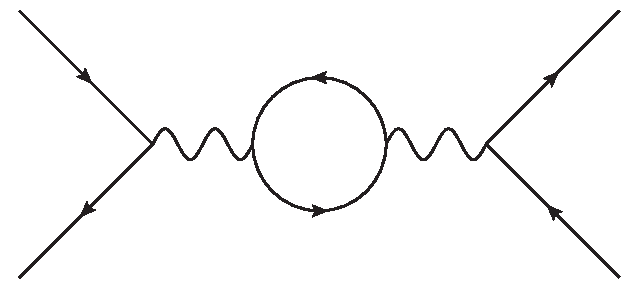
\includegraphics[width=0.6\textwidth]{figures/susyintro/epscattering_fermionloop.pdf}
		\caption{ }
		\label{fig:feynmandiagram_b}
	\end{subfigure}

	\begin{subfigure}[b]{0.45\textwidth}
		\centering
		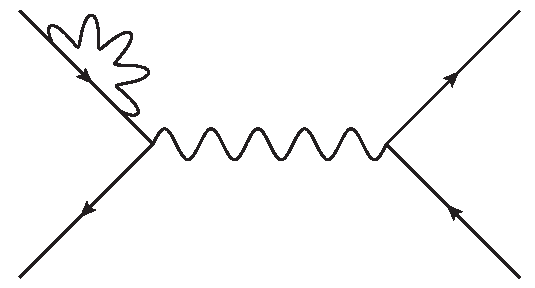
\includegraphics[width=0.6\textwidth]{figures/susyintro/epscattering_fermioncorr.pdf}
		\caption{ }
		\label{fig:feynmandiagram_c}
	\end{subfigure}
	\begin{subfigure}[b]{0.45\textwidth}
		\centering
		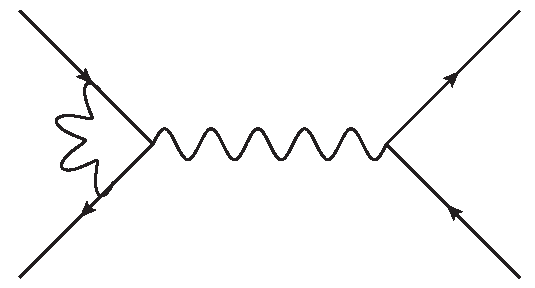
\includegraphics[width=0.6\textwidth]{figures/susyintro/epscattering_vertexcorr.pdf}
		\caption{ }
		\label{fig:feynmandiagram_d}
	\end{subfigure}
	\caption{Feynman diagrams of contributions to inelastic $e^+ e^-$ scattering. Made using \cite{Binosi:2003yf}.}
	\label{fig:feynmandiagram}
\end{figure}
The Feynman calculus associates each diagram with a specific mathematical expression called the Feynman amplitude $\mathcal{M}$ for that diagram. When several diagrams are included, the total amplitude for the process to the given order is the sum of the amplitudes from each diagram. The physical quantities of interest are obtained by integrating the amplitude (or its absolute square) over all spin and momentum configurations of the system.

\section{Renormalization}
\label{sec:renormalization}
The subleading diagrams, like those in fig.\  \ref{fig:feynmandiagram} (b--d), contain closed loops. These loops introduce extra momentum integrals into the calculations. Often, these integrals are divergent --- which is unacceptable from a physical viewpoint. The divergences can be understood and dealt with by using the techniques of {\it regularization} and {\it renormalization}. 
\subsection{Regularization}
Regularization is a means for parametrizing the divergence in terms of some small parameter $\epsilon$ which is zero in the physical limit. The most modern way to regularize a momentum integral is by using {\it dimensional regularization}: The original loop integral is an integral over four space-time dimensions. Dimensional regularization makes the substitution $4 \to d = 4-\epsilon$, so the integral becomes
\begin{align}
	\int d^4 \, k \to \int d^d \, k.
\end{align}
This integral is mathematically well-defined, and allows the divergences to be parametrized in terms of $\epsilon$.
\subsection{Renormalization}
When the divergence has been isolated and parametrized, it needs to be explained physically. This is done by the process of renormalizing the theory. For instance, in the case of the photon propagator in quantum electrodynamics, illustrated in fig.\ \ref{fig:feynmandiagram_b}, the dimensionally regularized expression for the leading-order loop correction to the propagator is proportional to
\begin{align}
	\int_0^1 dx \, x (1-x) \left( \frac{2}{\epsilon} - \log \left(m^2 - x(1-x)q^2 \right) + \mathrm{constant~terms} \right), \label{eq:divergent_loop_result}
\end{align}
which blows up as $\epsilon\to 0$. Renormalization is the claim that this infinity is a part of the {\it bare} physical constants which are present in the Lagrangian, in this case the electrical charge, whose bare value is denoted $e_0$. These bare parameters are not observable quantities, only parameters in the Lagrangian. What is observed is the {\it renormalized} charge $e = e_0 + \delta e$, where $\delta e$ is the infinite shift that cancels eq.\ \eqref{eq:divergent_loop_result}.

All the coupling constants of the Standard Model are renormalized. The renormalization introduces an {\it energy dependence} into the coupling constants, since the shift comes from loop corrections which depend on the energy of the process. For instance, the effective value of the electron charge in quantum electrodynamics, at some momentum $q$, is at one-loop order given as
\begin{align}
	e^2(q) = \frac{e_r^2}{1 - (e_r^2/6\pi^2)\log(q/M)},\label{eq:electron_charge_running}
\end{align}
where $e_r$ is some reference value for the charge, defined at the energy scale $q_r = M$. The fact that the coupling constants are not constant is referred to as the {\it running of the coupling constants}.

\subsection{The Callan-Symanzik equation}
The Callan-Symanzik, or {\it renormalization group} (RG) equation is the equation which describes the running of the coupling constants in a systematic way for any interaction in a quantum field theory. It is obtained by requiring that the Greens function for the interaction, $G$, {\it i.e.}\ the propagator, varies with the renormalization scale $M$ in such a way that the bare parameters of the Lagrangian is unchanged. For the example of massless QED, the Callan-Symanzik equation for a Green's function with $n$ electron fields and $m$ photon fields is \cite[p.\ 411]{Peskin-Schroeder}
\begin{align}
	\left[ M \frac{\partial}{\partial M} + \beta(e) \frac{\partial}{\partial e} + n\gamma_2(e) + m\gamma_3(e)\right] G^{(n,m)}(x_1, ..., x_n; M,e) = 0.\label{eq:callansymanzik}
\end{align}
The functions beta and gamma are defined as
\begin{align}
	\beta \equiv M\frac{\partial e}{\partial M} , \quad \gamma_i \equiv - M\frac{\partial \eta_i}{\partial M},
\end{align}
where $\delta\eta_i$ are the field-strength renormalization terms, shifting the field values of the electron and photon fields,
\begin{align}
	\psi \to (1 + \delta \eta_2) \psi \quad \mathrm{and} \quad A_\mu \to (1 + \delta\eta_3) A_\mu,
\end{align}
respectively. The Callan-Symanzik equation states that the combined effect of all the shifts in parameters induced by the renormalization should exactly weigh up for the shift in the Green's function itself, which is given by
\begin{align}
	G^{(n,m)} \to (1 + n\delta\eta_2 + m\delta\eta_3)G^{(n,m)}.
\end{align}
This is what is stated in eq.\ \eqref{eq:callansymanzik}. The Callan-Symanzik equation for other interactions, such as the $SU(3)$ quantum chromodynamics, may be derived similarily, but its complexity grows with the complexity of the interaction.

The primary quantities of interest from a phenomenological viewpoint are the beta and gamma functions. They describe the change in the coupling constant and other parameters as a function of renormalization scale, and in the case of QED they may be used to derive the formula \eqref{eq:electron_charge_running} for the running of the electromagnetic coupling constant $e$. Equation \eqref{eq:electron_charge_running} shows that the electromagnetic coupling constant increases as a function of the energy $q$. The same turns out to be true for the weak coupling constant, while the strong coupling constant of QCD decreases with increasing energy. This last fact is called {\it asymptotic freedom}, and means that the quarks and gluons are unbound by strong forces in the limit of high energy, or equivalently, short distances. 





\section[Motivations for extending the Standard Model]{Motivations for extending the\\ Standard Model}

Since the Standard Model is widely believed to be a low-energy effective model of some more fundamental high-energy theory, it is speculated that the three interactions of the Standard Model unite at a higher energy and act as a single interaction under some larger gauge group. However, when the three couplings are evolved to high energies using the Callan-Symanzik equations, they do not meet at a single point. This is seen by many as a flaw of the Standard Model. In the theory of Supersymmetry, the evolution of the couplings is altered, and they may meet at a single point. This effect is shown in fig.\ \ref{fig:coupling_unification}. Supersymmetry is discussed in more detail in the next chapter.
\begin{figure}[hbt]
	\centering
	\includegraphics[width=0.6\textwidth]{figures/susyintro/unification.eps}
	\caption{Evolution of the inverse fine structure constants $\alpha^{-1}_i = 4\pi/g_i$, for the cases of the Standard Model (dashed lines) and models with supersymmetry (solid lines). From \cite{Martin:1997ns}.}
	\label{fig:coupling_unification}
\end{figure}

Another issue with the Standard Model is that is has no candidate for particle dark matter. Observations over the last century have given strong evidence for the existence of some as yet unkown form of matter which is distributed in large quantites all over the universe --- in fact four times as much as our ordinary matter. It is widely believed that this dark matter is some form of particle. Dark matter interacts primarily, or possibly even solely, via gravitation, so the particle has to be colourless and electrically neutral, because the strength of these interactions would otherwise lead to the particle having been observed by now. It also has to be long-lived in order to explain the abundance of dark matter that we observe in the universe today. These restrictions rule out most of the Standard Model particles, with the exception of neutrinos. But neutrinos are known to be very light, almost massless, and calculations of early-universe dynamics show that they are too light to be candidates for dark matter. 

There is also a more technical problem with the Standard Model, related to the scalar Higgs field. As discussed in section \ref{subsec:feynmancalculus}, the calculations of parameters in a quantum field theory are subject to loop corrections. The Higgs mass parameter recieves corrections from loops containing all massive fermions, with the largest contribution coming from the top quark. The leading-order fermion contribution is shown in fig.\ \ref{fig:higgs_correction_a}.
\begin{figure}[htbp]
	\centering
	\begin{subfigure}[b]{0.49\textwidth}
		\centering
		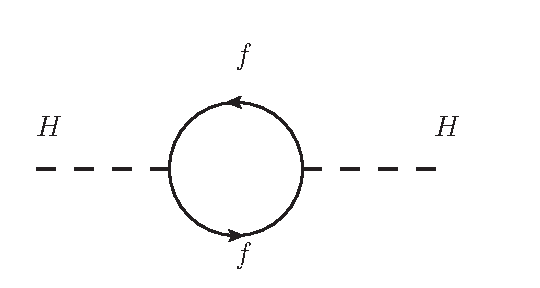
\includegraphics[width=0.6\textwidth]{figures/susyintro/higgs_top_loop.eps}
		\caption{ }
		\label{fig:higgs_correction_a}
	\end{subfigure}
	\begin{subfigure}[b]{0.49\textwidth}
		\centering
		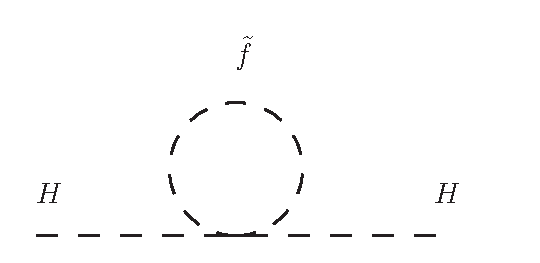
\includegraphics[width=0.6\textwidth]{figures/susyintro/higgs_stop_loop.eps}
		\caption{ }
		\label{fig:higgs_correction_b}
	\end{subfigure}
	\caption{Loop corrections to the Higgs mass. Subfigure (a) shows the leading Standard Model contributions, and subfig.\ (b) shows the corresponding supersymmetric contributions which cancel them.}
	\label{fig:higgs_correction}
\end{figure}

An alternative to the dimensional regularization technique discussed in section \ref{sec:renormalization} is to use a {\it momentum cutoff} $\Lambda$, which is infinite in the physical limit. One may argue that new physics should come into play at higher energy scales, such as the GUT scale, and therefore set the cutoff to a finite value, {\it e.g.}\ $\Lambda = M_{\mathrm{GUT}} \sim 10^{16}~\mathrm{GeV}$.

The fermions and vector bosons of the Standard Model also recieve corrections, but because of chiral and gauge symmetries, these can be shown to be at most logarithmically divergent in terms of $\Lambda$. For the scalar Higgs particle, there is no such ``protective symmetry'', and the loop integrals turn out to be quadratic in $\Lambda$. This is shown in appendix \ref{appendix:higgs_mass_loop_correction}. This means that the Higgs mass corrections, evaluated at {\it e.g.}\ $\Lambda = M_{\mathrm{GUT}}$, are many orders of magnitude larger than the observed Higgs mass of 126 GeV, implying very nearly exact cancellations among the correction terms. There is no symmetry in the Standard Model which says that such a cancellation should occur, so it appears to be an ``accident'' of nature. Such accidents are seen as unnatural, and this explanation is thus unsatisfactory from a theoretical viewpoint. This is referred to as the {\it hierarchy problem} of the Higgs mass. 

In supersymmetry, new scalar degrees of freedom enter into the loop corrections as illustrated in fig.\ \ref{fig:higgs_correction_b} for scalar ``sfermions'' $\tilde f$. The leading-order loop correction contributions from fermions and sfermions combined are 
\begin{align}
	\Delta m_H^2 = -\frac{|\lambda_f|^2}{8\pi^2}\Lambda^2 + \frac{\lambda_{\tilde f}}{16\pi^2}\Lambda^2 + \cdots\label{eq:higgs_mass_corrections}
\end{align}
to leading order in $\Lambda$, where $\Lambda$ is a high-momentum cutoff which regularizes the divergence in the loop integral, and $\lambda_{f/\tilde f}$ are the coupling strengths to fermions/sfermions. This is shown in appendix \ref{appendix:higgs_mass_loop_correction}. In supersymmetry, the coupling for a fermion $f$ is related to its sfermion partner by $|\lambda_f|^2 = \lambda_{\tilde f}$, and there are exactly two sfermions for each fermion. Thus, in supersymmetry, the corrections cancel each other in a natural way.






%%%%%%%%%%%%%%%%%%%%%%%%%%%%%%%%%%%%%%%%%%%%%%%%%%%%%%%%%%%%%%%%%%%%%%%%
\chapter{Supersymmetry}%%%%%%%%%%%%%%%%%
%%%%%%%%%%%%%%%%%%%%%%%%%%%%%%%%%%%%%%%%%%%%%%%%%%%%%%%%%%%%%%%%%%%%%%%%
\label{ch:susyintro}
The theory of supersymmetry (SUSY) is a proposed extension of the Standard Model which increases the number of degrees of freedom by introducing a symmetry between fermions and bosons, called a supersymmetry. The construction of supersymmetry is in some sense a two-step process, where one first derives the Lagrangian of a theory with complete symmetry between fermions and bosons, meaning that every bosonic degree of freedom gets a corresponding `supersymmetric' fermionic degree of freedom, and {\it vice versa}. These fields only differ in spin. But since, for example, scalar, colour charged particles with the same mass as the quarks are not observed in experiments, the symmetry cannot be exact. To make the theory physically viable, the supersymmetric partners must in most cases be significantly heavier than their Standard Model counterparts. This means that the supersymmetry must be a broken symmetry, and this breaking is in practice put into the theory ``by hand''.

In this chapter we will outline the construction of a supersymmetric theory. First, we introduce the group theoretic framework of the symmetries. We define the concept of superfields, fields transforming under representations of the supersymmetry group. We go on to construct a fully supersymmetric Lagrangian in the framework of the Minimal Supersymmetric Standard Model (MSSM). Then the breaking of SUSY is achieved by manually inserting so-called ``soft'' SUSY-breaking terms. Also, the concept of R-parity is introduced in order to ensure the stability of the proton. R-parity will also make the lightest supersymmetric particle a good dark matter candidate. From the broken SUSY Lagrangian, we extract the particle content --- identifying the familiar fields of the Standard Model as well as their supersymmetric counterparts. We then introduce a popular phenomenological model used to constrain and study the parameter space of the MSSM, and discuss its implications for the hierarchy of SUSY masses. This constrained model is subsequently adopted for the study of particular SUSY cascade decays, which is the topic for the remainder of the thesis. We will also review the current experimental status of SUSY. 

% The presentation is based on \cite{Batzing:2013} and \cite{Leinonen:2014}.

\section{Extending the Poincar\'{e} symmetry}
In the beginning of Chapter \ref{ch:SM_intro}, the Poincar\'{e} group was mentioned. It is the group of all Lorentz boosts and rotations, as well as all translations in spacetime. It is defined by its Lie algebra, called the {\it Poincar\'{e} algebra},
\begin{align}
	[M_{\mu\nu}, M_{\rho\sigma}] &= -i(g_{\mu\rho}M_{\nu\sigma} - g_{\mu\sigma}M_{\nu\rho} - g_{\nu\rho}M_{\mu\sigma} + g_{\nu\sigma}M_{\mu\rho})\\
	[P_\mu, P_\nu] &= 0\\
	[M_{\mu\nu}, P_\rho] &= -i(g_{\mu\rho}P_\nu - g_{\nu\rho}P_\mu),
\end{align}
where $M_{\mu\nu}$ is the generator of Lorentz boosts and rotations and $P_\mu$ is the momentum operator, the generator of translations. Any physical theory obeying Special Relativity must be invariant under the Poincar\'{e} group. It was shown in 1967 by Coleman and Mandula \cite{PhysRev.159.1251}, during attempts to unify Special Relativity with the observed global hadron flavour symmetry groups in a larger symmetry group structure, that there exists no Lie-algebra based extension of the Poincar\'{e} symmetry which includes the gauge groups of the Standard Model in a non-trivial way, {\it i.e.}\ a way by which the extended group cannot be decoupled as a direct product such that the groups do not couple to each other.

This prompted Haag, \L{}opusza\'{n}ski and Sohnius \cite{Haag1975257} to introduce the concept of a {\it superalgebra}. A superalgebra, or {\it graded} Lie algebra, $L$, is a direct sum of two Lie algebras $L_0$ and $L_1$, $L = L_0 \oplus L_1$, with a special binary operation called a {\it grading}. For $x_i \in L_i$, the grading operation is given by
\begin{align}
	x_i \cdot x_j = x_k \in L_{i+j~\mathrm{mod}\,2},
\end{align}
which means that $x_0 \cdot x_0 \in L_0$, $x_1 \cdot x_1 \in L_0$ and $x_0 \cdot x_1 \in L_1$. 

Haag {\it et. al.}\ constructed a superalgebra by combining the Poincar\'{e} algebra with an algebra spanned by four operators called {\it Majorana spinor charges}, represented by a two-component Weyl spinor $Q_A$ (to be defined shortly) and its hermitian conjugate $\bar Q_{\dot A}$. The resulting superalgebra is given by the (anti)commutation relations
\begin{align}
	[Q_A,P_\mu] &= [\bar Q_{\dot A}, P_\mu] = 0,\label{eq:susy_algebra_begin}\\
	[Q_A, M_{\mu\nu}] &= \sigma_{\mu\nu,A}^B Q_B,\\
	\{Q_A, Q_B\} &= \{\bar Q_{\dot A}, \bar Q_{\dot B} \} = 0\\
	\{Q_A, \bar Q_{\dot B} \} &= 2\sigma^\mu_{A \dot B} P_\mu,\label{eq:susy_algebra_end}
\end{align}
where $\sigma_\mu = (1_{2\times2},\sigma_i)$, with $\sigma_i$ the Pauli matrices and $\sigma_{\mu\nu} = \frac{i}{4}(\sigma_\mu \bar\sigma_\nu - \sigma_\nu \bar\sigma_\mu)$. It is possible to extend the superalgebra further by introducing more Majorana spinor charges, labeled $Q_A^\alpha$ for $\alpha=1,...,N$. For general $N$, this extension can be shown to be the largest possible extension of the Poincar\'{e} group. The extension defined by eqs.\ (\ref{eq:susy_algebra_begin}--\ref{eq:susy_algebra_end}) is called $N=1$ supersymmetry.

In the usual spinor representation of the Poincar\'{e} group, the fermion fields are represented as four-component Dirac spinors. It can be shown that the Poincar\'{e} group is isomorphic to $SL(2,\mathbb{C})\times SL(2,\mathbb{C})$, so it is possible to define the theory using the representations of this group instead. The $SL(2,\mathbb{C})$ group has two inequivalent fundamental representations by two-component spinors which are called {\it left- and right-handed Weyl spinors} and written as $\psi_A$ and $\bar\psi_{\dot A}$, respectively. 

The transformations corresponding to the superalgebra are called {\it supersymmetry transformations}.

\section{Superfields}
The objects transforming under supersymmetry transformations can be represented by {\it superfields}, which are functions defined on the {\it superspace} spanned by the spacetime coordinates $x^\mu$ and four anti-commuting Grassman numbers $\theta_A$ and $\bar\theta_{\dot A}$.  There are two important types of superfields, called chiral and vector superfields. Because of the anticommutativity, which means that any Grassman number squared vanishes, a function of a Grassman number, $f(\theta_A)$, has an all-order expansion given by
\begin{align}
	f(\theta_A) = a + b\theta_A.
\end{align}
Using this fact, a superfield $\Phi$ may generally be written as
\begin{align}
	\Phi = &f(x) + \theta^A\phi_A(x) + \bar\theta_{\dot A}\bar\chi^{\dot A}(x) + \theta \theta m(x)\\
	 &+ \bar\theta \bar\theta n(x) + \theta\sigma^\mu \bar\theta V_\mu(x) + \theta\theta\bar\theta_{\dot A}\bar\lambda^{\dot A}(x) + \bar\theta \bar\theta \theta^A \psi_A(x) + \theta \theta \bar\theta \bar\theta d(x).\nonumber
\end{align}
The different field components have the following properties: $f(x)$, $m(x)$ and $n(x)$ are complex (pseudo)scalars, $\psi_A(x)$ and $\phi_A(x)$ are left-handed Weyl spinors, $\bar\chi^{\dot A}(x)$ and $\bar\lambda^{\dot A}(x)$ are right-handed Weyl spinors, $V_\mu (x)$ is a complex Lorentz four-vector and $d(x)$ is a complex scalar.
% \begin{itemize}
% 	\item $f(x), m(x)$ and $n(x)$ are complex (pseudo)scalars
% 	\item $\psi_A(x)$ and $\phi_A(x)$ are left-handed Weyl spinors
% 	\item $\bar\chi^{\dot A}(x)$ and $\bar\lambda^{\dot A}(x)$ are right-handed Weyl spinors
% 	\item $V_\mu (x)$ is a Lorentz four-vector
% 	\item $d(x)$ is a complex scalar
% \end{itemize}

A supersymmetry transformation on a superfield $\Phi(x^\mu, \theta, \bar\theta)$ in terms of infinitesimal parameters $\xi_A$ and $\bar\xi^{\dot A}$ may be written
\begin{align}
	\delta_\xi \Phi &= \left( \xi^A \frac{\partial}{\partial \theta^A} + \bar\xi_{\dot A}\frac{\partial}{\partial \bar\theta_{\dot A}} + i\left[ \xi\sigma^\mu \bar\theta + \bar\xi \bar\sigma^\mu \theta  \right]\partial_\mu \right)\Phi\label{eq:susy_transformation}\\
	&= \Phi(x^\mu + i\xi\sigma^\mu\bar\theta + i\bar\xi \bar\sigma^\mu \theta, \theta + \xi, \bar\theta + \bar\xi) - \Phi(x^\mu, \theta, \bar\theta).\nonumber
\end{align}
A set of covariant derivatives are defined by
\begin{align}
	D_A = \frac{\partial}{\partial \theta^A} - i\sigma^\mu_{A \dot A}\bar\theta^{\dot A}\partial_\mu, \quad \bar D^{\dot A} = -\frac{\partial}{\partial \bar \theta_{\dot A}} + i\bar\sigma^{\mu,A \dot A}\theta_A \partial_\mu,
\end{align}
which can be shown to satisfy
\begin{align}
 	\delta_\xi (D_A \Phi) = D_A ( \delta_\xi \Phi), \quad \delta_\xi (D^{\dot A} \Phi ) = D^{\dot A} ( \delta_\xi \Phi),
 \end{align}
 so that they are indeed supersymmetrically covariant. In terms of these, a {\it left chiral} superfield $\Phi$ is defined by the condition
\begin{align}
	\bar D^{\dot A} \Phi = 0.
\end{align}
By substituting $y^\mu = x^\mu - i\theta\sigma^\mu \bar \theta$, the covariant derivative $\bar D^{\dot A}$ is given as
\begin{align}
	\bar D^{\dot A} = -\frac{\partial}{\partial \bar\theta_{\dot A}}.
\end{align}
This shows that a left-chiral superfield must be independent of $\bar \theta$ in these coordinates, so it may generally be written as
\begin{align}
	\Phi(y, \theta) = A(y) + \sqrt{2}\theta\psi(y) + \theta\theta F(y), 
\end{align}
thus containing two complex scalar fields and a left-handed Weyl spinor. Under the infinitesimal supersymmetry transformation defined in eq.\ \eqref{eq:susy_transformation}, the component field $F$ can be shown to transform into a total derivative. It will thus not contribute to the action, since all fields must vanish on the boundary at infinity. For this reason it is called an auxillary field. Thus we see that a left-chiral superfield contains two bosonic (scalar) degrees of freedom and two fermionic degrees of freedom contained in a left-handed Weyl spinor. Similar arguments may be applied to define a right-chiral superfield by the condition
\begin{align}
	D_A \Psi^\dag = 0,
\end{align}
and to show that it contains two auxillary and two proper scalar degrees of freedom, as well as a right-handed Weyl spinor. 

A {\it vector superfield} $V$ is defined by the condition
\begin{align}
	V^\dag = V.
\end{align}
This condition allows the field content
\begin{align}
	V = &f(x) + \theta^A\phi_A(x) + \bar\theta_{\dot A}\bar\chi^{\dot A}(x) + \theta \theta m(x) + \bar\theta \bar\theta m^*(x)\\
	 &+ \theta\sigma^\mu \bar\theta V_\mu(x) + \theta\theta\bar\theta_{\dot A}\bar\lambda^{\dot A}(x) + \bar\theta \bar\theta \theta^A \lambda_A(x) + \theta \theta \bar\theta \bar\theta d(x).
\end{align}
Here, the scalar fields $f(x)$ and $d(x)$, as well as the four-vector $V_\mu (x)$, are required to be real fields, thus halving their amount of degrees of freedom. There are auxillary degrees of freedom which may be removed by a gauge transformation. A vector superfield may be written in the {\it Wess-Zumino} gauge as
\begin{align}
	V_\mathrm{WZ} = (\theta \sigma^\mu \bar\theta) \left[ V_\mu(x) + i\partial_\mu (A(x) - A^*(x)) \right] + \theta\theta \bar\theta_{\dot A} \bar\lambda^{\dot A}(x) + \bar\theta \bar\theta \theta_A \lambda^A(x) + \theta\theta \bar\theta \bar\theta d(x),
\end{align}
where $A(x)$ is a complex scalar field obeying $A(x) + A^*(x) = 2\mathrm{Re}A(x) = -f(x)$. In this gauge, the vector superfield contains one real scalar field degree of freedom (d.o.f.) from $d(x)$, three gauge field d.o.f.'s from $\left[ V_\mu(x) + i\partial_\mu (A(x) - A^*(x)) \right]$ \footnote{$V_\mu$ has four d.o.f.'s, but one d.o.f.\ is removed by the gauge freedom of the imaginary part of $A(x)$} and four fermion d.o.f.'s from $\lambda(x)$ and $\bar\lambda(x)$.

\section{The unbroken supersymmetric Lagrangian}
\label{sec:unbroken_susy}
To obtain a theory which is supersymmetric, the action, given by
\begin{align}
 	S = \int d^4 x \mathcal{L},
 \end{align}
 needs to be invariant under SUSY transformations. As mentioned in the previous section, a total derivative has this property because its integral is determined by the boundary conditions, where it has to vanish. It can be shown that the highest-order component fields in $\theta$ and $\bar \theta$, {\it i.e.}\ the term proportional to $\theta\theta\bar\theta\bar\theta$, always has this property for both chiral and vector superfields and products thereof. Thus the invariance of the action may be ensured by redefining the Lagrangian using superfields such that\marginpar{A-komm: mention how L differs here from 2.18. Spør hva han mener.}
 \begin{align}
 	S = \int d^4 x \int d^4 \theta \mathcal{L},
 \end{align}
 where the last integral is over the four Grassman variables. This will project out only the desired terms, because of how the Grassman integral is defined. Thus the supersymmetric Lagrangian may be constructed from superfields and their products. It can be written generically as
 \begin{align}
 	\mathcal{L} = \mathcal{L}_{\theta\theta \bar\theta \bar\theta} + \theta \theta \mathcal{L}_{\bar\theta \bar\theta} + \bar\theta \bar\theta \mathcal{L}_{\theta \theta},
 \end{align}
 where the indices indicate the highest power of $\theta$ in each term.

The {\it superpotential} $W$ is defined as a product of left-chiral superfields,
 \begin{align}
 	W(\Phi) = L^i\Phi_i + \frac{1}{2}m^{ij}\Phi_i\Phi_j + \frac{1}{3}\lambda^{ijk}\Phi_i\Phi_j\Phi_k.
 \end{align}
The inclusion of higher-order field terms is ruled out by the condition of renormalizability, which forbids terms where the combined mass dimension of the fields are larger than four. Scalar, fermionic and auxillary fields have mass dimension one, 3/2 and 2, respectively, and the Grassman coordinates $\theta$ have dimension $-1/2$. The most general Lagrangian that can be written in terms of chiral superfields is
\begin{align}
	\mathcal{L} = \Phi_i^\dag \Phi_i + \bar\theta\bar\theta W(\Phi) + \theta\theta W(\Phi^\dag),
\end{align}
where the first term is called the kinetic term. 

The Lagrangian has to be gauge invariant. The general gauge transformation of a chiral superfield under a group $G$ is defined by
\begin{align}
	\Phi \overset{G}{\to} e^{-iq\Lambda^a T_a}\Phi,
\end{align}
where $T_a$ are the group generators, $q$ is the charge of $\Phi$ under $G$ and the gauge parameters $\Lambda_a$ themselves can be shown to be left-chiral superfields. The equivalent transformation for a right-chiral superfield $\Phi^\dag$ involves a right-chiral superfield gauge parameter $\Lambda_a^\dag$.

Analogously to the Standard Model, the supersymmetric gauge interactions are introduced as compensating terms to the gauge transformation of the chiral superfields. The analogue to the gauge boson fields are the vector superfields $V^a$, which are introduced into the kinetic terms of the Lagrangian by writing them as
\begin{align}
	\Phi^\dag_i e^{q V^a T_a}\Phi_i,
\end{align}
so that the kinetic term transforms as
\begin{align}
	\Phi_i^\dag e^{q V^a T_a}\Phi_i \overset{G}{\to} \Phi^\dag e^{iq(\Lambda^a)^\dag T_a}e^{qV^{'a}T_a}e^{-iq\Lambda^a T_a}\Phi,
\end{align}
which is invariant given that the vector superfields transform as
\begin{align}
	e^{qV^{'a} T_a} = e^{-iq(\Lambda^a)^\dag T_a}e^{qV^a T_a}e^{iq\Lambda^a T_a}.
\end{align}
For infinitesimal $\Lambda$, this is to leading order
\begin{align}
	V^{'a} = V^a + i(\Lambda^a - (\Lambda^a)^\dag) - \frac{1}{2}qf^a_{bc} V^b ((\Lambda^c)^\dag + \Lambda^c).
\end{align}
This gives for the vector component fields of the vector superfields, $V_\mu^a$,
\begin{align}
	V^a_\mu \overset{G}{\to} V^{'a}_\mu = V_\mu^a + i\partial_\mu(A^a - (A^a)^* - qf^{abc} V_\mu^b (A^c + (A^{c})^*).
\end{align}
With these definitions, it can be shown that the Standard Model couplings of fermions with bosons are recovered by defining the covariant derivative
\begin{align}
	D_\mu^i = \partial_\mu - \frac{i}{2} q_i V_\mu.
\end{align}

The SUSY Lagrangian terms containing the field strengths of the gauge fields are written as
\begin{align}
	\mathrm{Tr}[W^A W_A],
\end{align}
called the supersymmetric field strength, where $W_A$ and $\bar W_{\dot A}$ are left- and right-handed chiral superfields, respectively, given by
\begin{align}
	W_A &\equiv -\frac{1}{4}\bar D\bar D e^{-qV^aT_a} D_A e^{qV^a T_a},\\
	\bar W_{\dot A} &\equiv -\frac{1}{4} D D e^{-qV^aT_a} \bar D_{\dot A} e^{qV^a T_a}.
\end{align}
The general form of the SUSY Lagrangian is
\begin{align}
	\mathcal{L} = \Phi^\dag e^{qV^a T_a}\Phi + \bar\theta\bar\theta W(\Phi) + \theta\theta W(\Phi^\dag) + \frac{1}{2T(R)}\bar\theta\bar\theta \mathrm{Tr}(W^A W_A),
\end{align}
where $T(R)$, the {\it Dynkin index} of the representation of the gauge group, is a normalization constant.



\section{Supersymmetry breaking}
\label{sec:susybreaking}
Supersymmetry has to be a broken theory, at least in the low-energy limit, since supersymmetric particles with Standard Model masses are not observed. The breaking can be inserted into the SUSY Lagrangian ``by hand'', by explicitly adding terms that break SUSY and allow for mass splitting. The rationale for these terms is that the SUSY Lagrangian is only an effective Lagrangian where some heavy field has been integrated out, and that the breaking of SUSY occurs through this field at a higher scale through a spontaneous symmetry breaking mechanism similar to the Higgs mechanism in the Standard Model. There are several alternatives for the mechanisms of SUSY breaking, some of which are Planck-scale mediated SUSY breaking, gauge mediated SUSY breaking and anomaly mediated SUSY breaking. Whichever of the mechanisms is chosen, there are only a finite set of terms that may be added to the Lagrangian without reintroducing the hierarchy problems of the Higgs mass loop corrections. They are called {\it soft} SUSY breaking terms, required to have couplings of mass dimension one or higher, and may in the most general form be written
\begin{align}
	\mathcal{L}_\mathrm{soft} = &-\frac{1}{4T(R)}M\theta\theta\bar\theta\bar\theta \mathrm{Tr} [W^A W_A] - \frac{1}{6}a_{ijk} \theta\theta\bar\theta\bar\theta\Phi_i \Phi_j \Phi_k\nonumber\\
	&-\frac{1}{2}b_{ij} \theta\theta\bar\theta\bar\theta\Phi_i \Phi_j - t_i \theta\theta\bar\theta\bar\theta \Phi_i + \mathrm{h.c.}\\
	&-m_{ij} \theta\theta\bar\theta\bar\theta \Phi_i^\dag \Phi_j.\nonumber
\end{align}
In terms of the component fields of the superfields, the soft Lagrangian may be written
\begin{align}
	\mathcal{L}_\mathrm{soft} = &-\frac{1}{2} M\lambda^A\lambda_A - \left( \frac{1}{6} a_{ijk} A_i A_j A_k + \frac{1}{2} b_{ij} A_i A_j + t_i A_i + \frac{1}{2} c_{ijk} A^*_i A_j A_k + \mathrm{c.c.}\right)\\
	&- m_{ij}^2 A_i^* A_j.\nonumber
\end{align}
Since this contains both Weyl spinor fields $\lambda_A$ and scalar fields $A_i$, the soft terms may be used to modify masses and couplings of the superpartner scalar and fermionic fields which will appear below.



\section[The Minimal Supersymmetric Standard Model]{The Minimal Supersymmetric Standard\\ Model}
The Minimal Supersymmetric Standard Model (MSSM) is the minimal supersymmetric theory which contains the field content of the Standard Model. It is constructed by choosing superfields in accordance with the requirements deduced in the previous sections. To construct a Dirac fermion, we use one left-chiral and one right-chiral superfield together. This gives the four fermionic degrees of freedom that a Dirac fermion and its antiparticle require. Since each chiral superfield also contains two scalar degrees of freedom (after removing the auxillary fields), this introduces two scalar particle-antiparticle pairs, which are called the supersymmetric partners, or {\it superpartners}, of the Dirac fermion. An important point is that all superfield components must have the same charge under all gauge groups, due to the way the gauge transformation was defined. This means that the scalar fields generally will be charged. 

The superfields for the charged leptons are denoted $l_i$ and $\bar E_i$ for the left- and right-chiral superfields, respectively, and the left-handed neutrino superfields are denoted $\nu_i$. Here, $i=1,2,3$ is a generation index. The $SU(2)_L$ doublet of the Standard Model is recovered by setting $L_i = (\nu_i, l_i)$. The quark superfields are denoted $u_i$, $\bar U_i$, $d_i$ and $\bar D_i$, where $Q_i = (u_i, d_i)$ makes the $SU(2)_L$ doublet.

The gauge boson fields come from the vector superfields, each of which also contains two Weyl-spinor fields of opposite handedness. To obey gauge invariance, $n^2-1$ vector superfields are required for each of the $SU(n)$ groups just as in the Standard Model, {\it i.e.}\ gauge invariance under $U(1)_Y\times SU(2)_L \times SU(3)_C$ requires 1+3+8 vector superfields.\footnote{Again, $n^2$ rather than $n^2-1$ for the $U(1)$ group.} These are denoted $B^0$, $W^a$ and $C^a$, respectively. The Weyl spinor fields, the superpartners of the gauge fields, are written as $\tilde B^0$, $\tilde W^0$ and $\tilde g$, respectively. In the literature, these are referred to as {\it bino}, {\it wino} and {\it gluino}. 

The MSSM requires two Higgs superfield $SU(2)_L$ doublets to be able to give mass to both up- and down-type quarks. In the Standard Model, the same Higgs doublet can be used for both types by rotating the components using the $SU(2)_L$ generators, but this is not possible in SUSY because it would mix left- and right-handed superfields. The Higgs doublets in the MSSM are
\begin{align}
	H_u = \begin{pmatrix}
		H_u^+ \\ H_u^0
	\end{pmatrix}, \quad H_d = \begin{pmatrix}
		H_d^0 \\ H_d^-
	\end{pmatrix}.
\end{align}
This introduces several additional Higgs scalars into the model, as well as their fermionic superpartner fields.

Using the fields listed above, the MSSM Lagrangian $\mathcal{L}_\mathrm{MSSM}$ may be constructed, subject to the rules for a general gauge invariant SUSY Lagrangian that were derived in sections \ref{sec:unbroken_susy} and \ref{sec:susybreaking}. This gives rise to kinetic terms, superpotential terms, supersymmetric field strength terms and soft SUSY breaking terms. The total MSSM Lagrangian is
\begin{align}
	\mathcal{L} = \mathcal{L}_\mathrm{kin} + W + \mathcal{L}_V + \mathcal{L}_\mathrm{soft}.
\end{align}
The kinetic terms are
\begin{align}
	\mathcal{L}_\mathrm{kin} = &L_i^\dag e^{\frac{1}{2}g\sigma W - \frac{1}{2}g'B} L_i + Q_i^\dag e^{\frac{1}{2}g_s \lambda C + \frac{1}{2}g\sigma W + \frac{1}{3}\cdot \frac{1}{2}g'B}Q_i\nonumber \\
	&+ \bar U_i^\dag e^{\frac{1}{2}g_s \lambda C - \frac{4}{3}\cdot \frac{1}{2}g'B}\bar U_i + \bar D_i^\dag e^{\frac{1}{2}g_s \lambda C + \frac{2}{3}\cdot \frac{1}{2}g'B}\bar D_i \\
	&+ \bar E_i^\dag e^{2\frac{1}{2}g'B}\bar E_i + H_u^\dag e^{\frac{1}{2}g\sigma W + \frac{1}{2} g' B} H_u + H_d^\dag e^{\frac{1}{2}g\sigma W - \frac{1}{2}g'B} H_d,\nonumber
\end{align}
where $g'$, $g$ and $g_s$ are the coupling constants of $U(1)_Y$, $SU(2)_L$ and $SU(3)_C$, respectively. The hypercharge under $U(1)_Y$ is assigned in units of $\frac{1}{2}g'$ as a convention. Also, factors of $\frac{1}{2}$ are used in the transformations of $SU(2)_L$ and $SU(3)_C$ to avoid accumulation of numerical factors because of how the generators are defined. With these conventions, the electroweak relationship between electric charge $Q$, hypercharge $Y$ and weak isospin $T_3$ is
\begin{align}
	Q = \frac{Y}{2} + T_3.
\end{align}
The field strength terms are 
\begin{align}
	\mathcal{L}_V = &\frac{1}{2}\mathrm{Tr} \left\{ W^A W_A \right\} \bar\theta\bar\theta + \frac{1}{2}\mathrm{Tr} \left\{ C^A C_A \right\} \bar\theta\bar\theta + \frac{1}{4}B^A B_A \bar\theta\bar\theta + \mathrm{h.c.},
\end{align}
where the field strengths are given as
\begin{align}
	W_A &= -\frac{1}{4}\bar D \bar D e^{-W} D_A e^W,  	&W = \frac{1}{2}g\sigma^a W^a,\\
	C_A &= -\frac{1}{4}\bar D \bar D e^{-C} D_A e^C,  	&C = \frac{1}{2}g_s \lambda^a C^a,\\
	B_A &= -\frac{1}{4}\bar D \bar D D_A B,  			&B = \frac{1}{2}g' B^0.
\end{align}
The MSSM superpotential $W$ is
\begin{align}
	W = &\mu H_u H_d + \mu'_i L_i H_u + y_{ij}^e L_i H_d E_j y_{ij}^u Q_i H_u \bar U_j + y_{ij}^d Q_i H_d \bar D_j \label{eq:mssm_superpotential} \\
		&+\lambda_{ijk}L_i L_j \bar E_k + \lambda'_{ijk} L_i Q_j \bar D_k + \lambda''_{ijk} \bar U_i \bar D_j \bar D_k.\nonumber
\end{align} 
The SUSY breaking soft terms of the MSSM are, in component fields,
\begin{align}
	\mathcal{L}_\mathrm{soft} = &\left( -\frac{1}{2}M_1 \tilde B \tilde B - \frac{1}{2}M_2 \tilde W^{i,A} \tilde W^i_A - \frac{1}{2}M_3 \tilde g^{a,A}\tilde g^a_A + \mathrm{c.c.} \right)\nonumber\\
	+ &\left(-a_{ij}^e \tilde L_i H_d {\tilde e^*}_{iR} - a_{ij}^u \tilde Q_i H_u \tilde u^*_{iR} - a_{ij}^d \tilde Q_i H_d \tilde d^*_{jR} + \mathrm{c.c.} \right)\\
	- &(m_{ij}^L)^2 \tilde L_i^\dag \tilde L_j - (m_{ij}^e)^2 {\tilde e_{iR}^*} {\tilde e_{jR}} - (m_{ij}^Q)^2 \tilde Q_i^\dag \tilde Q_j \nonumber \\
	- &(m_{ij}^u)^2 {\tilde u_{iR}^*} {\tilde u_{jR}} - (m_{ij}^d)^2 {\tilde d_{iR}^*} {\tilde d_{jR}} - m^2_{H_u} H^\dag_u H_u - m^2_{H_d} H^\dag_d H_d.\nonumber
\end{align}
The soft terms constitute the main contributions to the superpartner masses. 

An important feature of the MSSM is that the superpartners inherit the couplings of their Standard Model counterparts, since they belong to the same superfields.

\subsection{R-parity}
The superpotential in eq.\ \eqref{eq:mssm_superpotential} contains terms which break lepton and baryon number conservation, namely $LH_u$, $LLE$ and $LQ\bar D$. If the couplings for these terms are large, they allow for proton decay, which is experimentally very heavily constrained, with a lifetime of $\tau_\mathrm{proton} > 10^{33} ~\mathrm{yr}$. To avoid this, it is conventional to introduce the concept of {\it R-parity}, which gives an explanation for why these terms are zero.

R-parity is a multiplicative quantum number which is assumed to be conserved in all SUSY interactions. Formally, a particle has R-parity given by
\begin{align}
	R = (-1)^{2s + 3B + L},
\end{align}
where $s$ is the particle's spin, $B$ its baryon number and $L$ its lepton number. The important point is that all Standard Model particles have $R=+1$ while all superpartners have $R = -1$. This leads to the very important prediction that superpartner particles only can be produced and annihilated in pairs. In particular, it means that the lightest superpartner (LSP) must be stable against decay. This makes the LSP very attractive as a candidate for dark matter, if it is electrically neutral and has no colour charge. In a SUSY scenario with conservation of R-parity, the supersymmetric particles will typically decay in {\it cascades} down to the LSP, emitting multiple Standard Model particles along the way.

\section{Radiative electroweak symmetry breaking}
The scalar potential of the MSSM Higgs fields is, in terms of component fields,
\begin{align}
	V(H_u, H_d) = 	&|\mu|^2 \left( |H_u^0|^2 + |H_u^+|^2 + |H_d^0|^2 + |H_d^-|^2 \right)\nonumber \\
					&+ \frac{1}{8} \left( g^2 + g'^2 \right) \left( |H_u^0|^2 + |H_u^+|^2 - |H_d^0|^2 - |H_d^-|^2 \right)\nonumber \\
					&+ \frac{1}{2} g^2 |H_u^+ H_d^{0*} + H_u^0 H_d^{-*}|^2\label{eq:mssm_higgspotential}\\
					&+ m_{H_u}^2 \left( |H_u^0|^2 + |H_u^+|^2 \right) + m_{H_d}^2 \left( |H_d^0|^2 + |H_d^+|^2 \right)\nonumber \\
					&+ \left[b\left(H_u^+ H_d^- - H_u^0 H_d^0\right) + \mathrm{c.c.}\right].\nonumber
\end{align}
It can be shown that a necessary and sufficient set of conditions for achieving spontaneous electroweak symmetry breaking in this potential is \cite{Batzing:2013}
\begin{align}
	b^2 &> \left( |\mu|^2 + m_{H_u}^2 \right) \left( |\mu|^2 + m_{H_d}^2 \right),\label{eq:rewsb-cond1}\\
	2b &< 2|\mu|^2 + m_{H_u}^2 + m_{H_d}^2.\label{eq:rewsb-cond2}
\end{align}

Like any quantum field theory, the MSSM is subject to renormalization, which induces the running of the coupling constants and masses of the model as discussed in Chapter \ref{ch:SM_intro}. In particular, the mass parameters $m_{H_{u/d}}$ for the Higgs doublets, which come from soft breaking terms in the Lagrangian, run with energy. To break the electroweak symmetry, {\it i.e.}\ satisfy eqs.\ (\ref{eq:rewsb-cond1}--\ref{eq:rewsb-cond2}), it is assumed that these are equal at some high scale, and run down. It can be shown that the beta functions which determine the running are given by
\begin{align}
	16\pi^2 \beta_{m_{H_u}^2} = 6|y_t|^2\left( m_{H_u}^2 + ( m_{33}^Q)^2 + (m_{33}^u)^2 \right),\\
	16\pi^2 \beta_{m_{H_d}^2} = 6|y_b|^2\left( m_{H_d}^2 + ( m_{33}^Q)^2 + (m_{33}^d)^2 \right),
\end{align}
where $y_t$ and $y_b$ are the top and bottom Yukawa couplings, respectively. Because the top Yukawa coupling is much larger than the bottom one, the $m_{H_u}$ parameter runs down much faster with energy and becomes negative, facilitating the symmetry breaking given by eqs.\ (\ref{eq:rewsb-cond1}--\ref{eq:rewsb-cond2}) This is called {\it radiative electroweak symmetry breaking}, and gives an explanation for the Higgs mechanism.

As a result of the symmetry breaking, the neutral components of both the Higgs doublets acquire a non-vanishing vacuum expectation value, $v_u = \langle H_u^0 \rangle$ and $v_d = \langle H_d^0 \rangle$, respectively. These must relate to the vector boson masses of the Standard Model as
\begin{align}
	v_u^2 + v_d^2 = \frac{2m_Z^2}{g^2 + g^{'2}} \approx (174 ~\mathrm{GeV})^2.
\end{align}
The remaining free parameter is conventionally parametrized as
\begin{align}
	\tan \beta \equiv \frac{v_u}{v_b}.
\end{align}

\section{Particle phenomenology of the MSSM}

 \begin{table}[hbt]
 \centering
 	\begin{tabular}{l |c | c | r}
 		Standard model particles\footnote{Plus the extended Higgs sector} & Spin & Superpartners & Spin\\
 		\hline
 		$e, \mu, \tau$ & 1/2 & $\tilde e_L, \tilde e_R, \tilde \mu_L, \tilde \mu_R, \tilde \tau_1, \tilde \tau_2$ & 0\\
 		\hline
 		$\nu_e, \nu_\mu, \nu_\tau$ & 1/2 & $\tilde \nu_{e,L}, \tilde \nu_{e,R}, \tilde \nu_{\mu,L}, \tilde \nu_{\mu,R}, \tilde \nu_{\tau,L}, \tilde \nu_{\tau,R}$ & 0\\
 		\hline
 		$u, d, s, c$ & 1/2 & $\tilde u_L, \tilde u_R, \tilde d_L, \tilde d_R, \tilde s_L, \tilde s_R, \tilde c_L, \tilde c_R$ & 0\\
 		\hline
 		$b, t$ & 1/2 & $\tilde b_1, \tilde b_2, \tilde t_1, \tilde t_2$ & 0\\
 		\hline
 		$h, H, A, H^\pm$ & 0 & $\chi_1^0, \chi_2^0, \chi_3^0, \chi_4^0$ & 1/2\\
 		$B^0, W^{1,2,3}$ & 1 & $\chi_1^\pm, \chi_2^\pm$ & 1/2\\
 		\hline
 		$g$ & 1 & $\tilde g$ & 1/2
 	\end{tabular}
 	\caption{Summary of MSSM particle and sparticle content.}
 	\label{table:MSSM_particles}
 \end{table}
The total particle content of the MSSM is as follows: \marginpar{These paragraphs could use a polish, they don't flow well}

The Standard Model particles are present: electrons, muons, taus and their corresponding neutrinos; the up, down, strange, charm, bottom and top quarks; the photon, Z boson and W bosons and gluons; and the Higgs boson. 

In addition to the Standard Model Higgs $h$, there are four other scalar Higgs particles with positive R-parity, labeled $H$, $H^\pm$ and $A$. $H$ is identical to $h$ except for its larger mass, and is therefore termed ``heavy Higgs'', in contrast to the ``light Higgs'' $h$ of the Standard Model. The other neutral field $A$ is a pseudo-scalar.

All the Standard Model particles get superpartners, often termed {\it sparticles}. For the gluons, they are called gluinos and labeled $\tilde g$. The partners of the $B^0$ and $W^a$ fields, which in the Standard Model make up the photon, $Z$ and $W^\pm$, mix with the superpartner Higgs fields to form four neutral Majorana fermions called neutralinos, labeled $\tilde\chi_i^0$, $i=1,...,4$, and two charged fermion-antifermion pairs called charginos, $\tilde\chi_i^\pm$, $i=1,2$. Each of the Standard Model fermions get two corresponding scalar particles with the same gauge charges. For the first two generations, the mass eigenstates split to good approximation into one left-chiral and one right-chiral fermion, such that {\it e.g.}\ the superpartners of the up quark $u$ are labeled $\tilde u_R$ and $\tilde u_L$. For the third-generation fermions, the chiral approximation is cruder, so these mass eigenstates are just numbered, {\it e.g.}\ $\tilde b_1$ and $\tilde b_2$ for the $b$ quark. A summary of the MSSM particle content is shown in table \ref{table:MSSM_particles}.

 The superpartner fields are members of the same superfields as their standard model partners. Therefore, they inherit the couplings of their partners. This is very useful when drawing Feynman diagrams for processes, since intuition from the Standard Model can be applied through {\it supersymmetrization} of the diagrams. For instance, the fermion-fermion-gauge boson vertices (fig.\ \ref{fig:feynmandiagram_supersymmetrization_a}) of the Standard Model have supersymmetrized fermion-sfermion-gaugino and sfermion-sfermion-gauge boson versions (figs.\ \ref{fig:feynmandiagram_supersymmetrization} b and c). (But {\it not} sfermion-sfermion-gaugino, because of R-parity.) 
 \begin{figure}[htbp]
	\centering
	\begin{subfigure}[b]{0.45\textwidth}
		\centering
		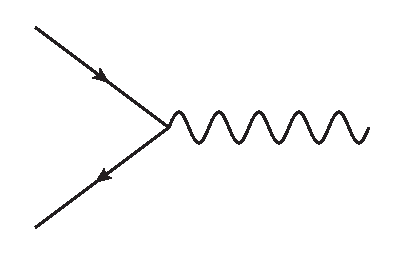
\includegraphics[width=0.6\textwidth]{figures/susyintro/ffg_vertex.eps}
		\caption{ }
		\label{fig:feynmandiagram_supersymmetrization_a}
	\end{subfigure}

	\begin{subfigure}[b]{0.45\textwidth}
		\centering
		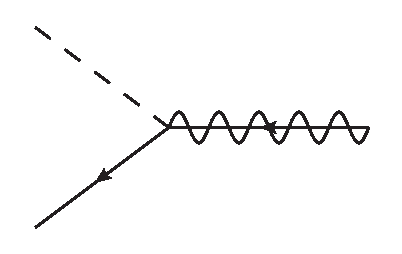
\includegraphics[width=0.6\textwidth]{figures/susyintro/sfg_vertex.eps}
		\caption{ }
		\label{fig:feynmandiagram_supersymmetrization_b}
	\end{subfigure}
	\begin{subfigure}[b]{0.45\textwidth}
		\centering
		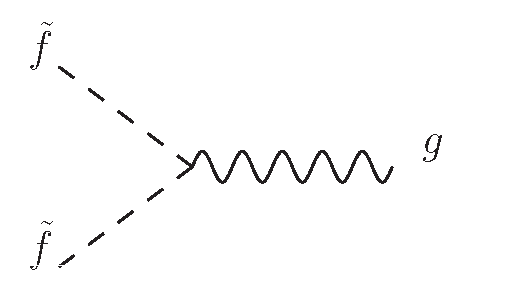
\includegraphics[width=0.6\textwidth]{figures/susyintro/ssg_vertex.eps}
		\caption{ }
		\label{fig:feynmandiagram_supersymmetrization_c}
	\end{subfigure}
	\caption{Feynman diagrams of a {\it fermion-fermion-gauge boson} vertex {\bf (a)} and the supersymmetrized {\it fermion-sfermion-gaugino} {\bf (b)} and {\it sfermion-sfermion-gauge boson} {\bf (c)} vertices.}
	\label{fig:feynmandiagram_supersymmetrization}
\end{figure}

An important consequence of the coupling inheritance is that the gaugino fields $\tilde\chi_i^{0/\pm}$ will couple differently depending on the mass mixing matrix. Since the wino field inherits the left-chiral $SU(2)_L$ coupling, the chirality of the couplings of the four neutralinos may differ considerably if the mass eigenstates are close to the gauge eigenstates. In the parameter point used for the analysis in the coming chapters, the second-generation neutralino consists of a large wino part, and this means that it has a small coupling to right-chiral quarks. 

 \subsection{Sparticle masses}
 The main contributions to the sparticle masses naturally come from the soft terms, since these are responsible for the symmetry breaking which would otherwise give Standard Model masses to sparticles. The mass parameters from these terms are the gaugino mass terms $M_{1,2,3}$, the sfermion mass terms $m_{ij}$ and the Higgs terms $m_{H_{u/d}}$. Additionally, the parameter $\mu$ from the superpotential term coupling the Higgs doublets together in the unbroken SUSY Lagrangian contributes.
 \begin{itemize}
 	\item At tree level, the different Higgs masses (which have positive R-parity) are
 	\begin{align}
 		m_A^2 &= 2|\mu|^2 + m^2_{H_u} + m^2_{H_d},\label{eq:mssm_higgs_masses1}\\
 		m^2_{h,H} &= \frac{1}{2} \left( m_A^2 + m_Z^2 \pm \sqrt{(m_A^2 - m_Z^2)^2 + 4m_Z^2m_A^2\sin^2 2\beta} \right),\label{eq:mssm_higgs_masses2}\\
 		m^2_{H^\pm} &= m_A^2 + m_W^2.
 	\end{align}
 	\item The gluino mass $m_{\tilde g}$ is given as
 	\begin{align}
 		m_{\tilde g} = M_3 \left[ 1 + \frac{\alpha_s}{4\pi}\left( 15 + 6\ln\frac{\mu}{M_3} + \sum_{\mathrm{all} ~\tilde q} A_{\tilde q} \right)\right],
 	\end{align}
 	where $A_{\tilde q}$ are the squark loop contributions given by
 	\begin{align}
 		A_{\tilde q} = \int_0^1 dx \, x \ln\left( x \frac{m^2_{\tilde q}}{M_3^2} + (1-x)\frac{m_q^2}{M_e^2} - x(1-x) - i\epsilon \right).
 	\end{align}%\marginpar{Not really sure what $M_e$ is...}
 	\item The neutralinos $\tilde\chi_i^0$ are the mass eigenstates of the bino, wino and higgsino fields. In the gauge eigenstate basis, where $\tilde\chi^{0} = (\tilde B^0, \tilde W^0, \tilde H_d^0, \tilde H_u^0)^T$, the mass matrix may be written
 	\begin{align}
 		M_{\tilde \chi^0} = \begin{pmatrix}
 			M_1 & 0 & - c_\beta s_{\theta_W} m_Z &  s_\beta s_{\theta_W} m_Z \\
 			0 & M_2 &  c_\beta c_{\theta_W} m_Z & - s_\beta c_{\theta_W} m_Z\\
 			- c_\beta s_{\theta_W} m_Z &  s_\beta s_{\theta_W} m_Z & 0 & -\mu \\
			 c_\beta c_{\theta_W} m_Z & - s_\beta c_{\theta_W} m_Z & -\mu & 0
 		\end{pmatrix},
 	\end{align}
 	where $c_x = \cos x$ and $s_x = \sin x$. For a given parameter choice, this matrix must be diagonalized to find the neutralino masses.
 	\item The charginos $\tilde\chi_i^\pm$ have analogous structure. In the gauge eigenstate basis $\tilde \chi^{\pm} = (\tilde W^+, \tilde H_u^+, \tilde W^-, \tilde H_d^-)^T$, the mass matrix is
 	\begin{align}
 		M_{\tilde \chi^\pm} = \begin{pmatrix}
 			0 & 0 & M_2 & \sqrt{2} c_\beta m_W  \\
 			0 & 0 & \sqrt{2} s_\beta m_W & \mu \\
 			M_2 & \sqrt{2} s_\beta m_W & 0 & 0\\
 			\sqrt{2} s_\beta m_W & \mu & 0 & 0
 		\end{pmatrix}.
 	\end{align}
 	\item The first two generations of {\it sfermions}, superpartners of the Standard Model fermions, get masses according to
 	\begin{align}
 		m^2_F = m^2_{F,\mathrm{soft}} + \Delta_F,
 	\end{align}
 	where $m^2_{F,\mathrm{soft}}$ is the mass term from the soft term of the form $-m^2_F F^\dag F$ and $\Delta_F$ is given by
 	\begin{align}
 		\Delta_F = (T_{3F} - Q_F \sin^2\theta_W)\cos 2\beta \, m^2_Z,
 	\end{align}
 	where $T_{3f}$ and $Q_F$ are the weak isospin and electric charge, respectively, of the left-handed supermultiplet to which the sfermion belongs. The masses are then {\it e.g.}\
 	\begin{align}
 		&m^2_{\tilde e_L} = m^2_{L_1} + \Delta \tilde e_L,\\
 		&m^2_{\tilde e_R} = m^2_{e_R} + \Delta \tilde e_R.
 	\end{align}
 	The mass-splitting between same-generation sleptons and squarks are universal and given by {\it e.g.}\ %\marginpar{Is it the same for right-handeds? Check, or don't mention?}
 	\begin{align}
 		m^2_{\tilde e_L} - m^2_{\tilde \nu_L} = m^2_{\tilde d_L} - m^2_{\tilde u_L} = -\cos 2\beta \, m_W^2.
 	\end{align}
 	\item The third-generation sfermions get more complicated masses, given for {\it e.g.}\ the stop squark by the mass matrix in the chiral gauge eigenstate basis $\tilde t = (\tilde t_L, \tilde t_R)^T$
 	\begin{align}
 		m^2_{\tilde t} = \begin{pmatrix}
 			m^2_{Q_3} + m_t^2 + \Delta \tilde u_L & v((a_{33}^u)^* \sin\beta - \mu y_t \cos\beta)\\
 			v(a_{33}^u \sin\beta - \mu^* y_t \cos\beta) & m^2_{u3} + m^2_t + \Delta \tilde u_R
 		\end{pmatrix},
 	\end{align}
 	which can be diagonalized to find the mass eigenstates. The reason that the third-generation sfermions have more complicated mass matrices is that the Yukawa couplings are larger, giving non-negligible contributions to the masses.
 \end{itemize}

 \section{Gauge unification and mass hierarchies}
 It was mentioned in the introduction that one very appealing feature of supersymmetry is that the coupling constants of the electromagnetic, weak and strong interactions can be made to unite at a high energy scale. In the MSSM, this scale, called the ``grand unification scale'' (GUT), is $m_\mathrm{GUT} \approx 2\times 10^{16} ~\mathrm{GeV}$. If we assume that the grand unified gauge group is $SU(5)$ or $SO(10)$\footnote{$SO(n)$ is the {\it special orthogonal group}, given in the defining matrix representation as the group of all orthogonal $n\times n$ matrices of determinant 1.}, then we can take the three gauge couplings of the grand unified theory to be \cite{Batzing:2013}
 \begin{align}
 	g_1 = \sqrt{\frac{5}{3}}g', \quad g_2 = g, \quad g_3 = g_s.
 \end{align}
 It can be shown that the $\beta$-functions of the gauge couplings $g_i$ and the gaugino soft mass parameters $M_i$ are
 \begin{align}
 	\beta_{g_i}|_\mathrm{1-loop} &= \frac{1}{16\pi^2} b_i g_i^3,\\
 	\beta_{M_i} |_\mathrm{1-loop} &= \frac{1}{8\pi^2}g_i^2 M_i b_i.
 \end{align}
The ratios $M_i/g_i^2$ for all three parameter pairs are scale independent at one-loop order. To see this, it is convenent to write the $\beta$-functions as 
 \begin{align}
 	\beta_X \equiv \frac{d}{dt}X
 \end{align}
 for a running variable $X$, where $t = \log \mu$ is the {\it scale parameter} for the renormalization scale $\mu$. If we define
 \begin{align}
 	R = \frac{M_i}{g_i^2},
 \end{align}
 then
 \begin{align}
 	\beta_R = \frac{dR}{dt} &= \frac{(\frac{d}{dt}M_i)g_i^2 - M_i\frac{d}{dt}g_i^2}{g_i^4} \\
 	&= \frac{\frac{1}{8\pi^2}g_i^2M_i b_i g_i^2 - M_i 2g_i \frac{1}{16\pi^2}g_i^3 b_i}{g_i^4} = 0, \nonumber
 \end{align}
 which proves the claim. 

 By assuming that the coupling constants $g_i$ unite to the value $g_u$ at the GUT scale, and that the gaugino masses $M_i$ have the common value $m_{1/2}$ at the same scale, then it follows that
 \begin{align}
 	\frac{M_1}{g_1^2} = \frac{M_2}{g_2^2} = \frac{M_3}{g_3^2} = \frac{m_{1/2}}{g_u}.
 \end{align}
 In terms of the electromagnetic and strong fine-structure constants $\alpha$ and $\alpha_s$, and the Weinberg angle $\theta_W$, this gives
 \begin{align}
 	M_3 = \frac{\alpha_s}{\alpha}\sin^2\theta_W M_2 = \frac{3}{5}\frac{\alpha_s}{\alpha} \cos^2\theta_W M_1.
 \end{align}
 At a scale of $1 ~\mathrm{TeV}$, it evaluates to 
 \begin{align}
 	M_3 : M_2 : M_1 = 6 : 2 : 1.
 \end{align}
 This propagates into the mass formulas to predict the approximate mass relationships
 \begin{align}
 	m_{\tilde g} \approx 6m_{\tilde \chi_1^0} \quad \mathrm{and} \quad m_{\tilde \chi_2^0} \approx m_{\tilde \chi_1^\pm} \approx 2m_{\tilde \chi_1^0}.
 \end{align}

\section{The Constrained MSSM}
\label{sec:cmssm}
The available parameter space of the general MSSM is very large, of the order 100 free parameters. The reason for the vast number of parameters are the soft SUSY breaking terms, which contain coupling parameters for all the extra terms without any {\it a priori} way to relate them. It is therefore conventional to make some restricting assumptions. A much-studied restriction is the {\it Constrained MSSM} (CMSSM), also known as {\it minimal supergravity} (mSUGRA). This model is constructed by assuming that SUSY breaking is mediated by some mechanism of gravity at the Planck scale of $M_P = 2.4\times 10^{18} ~\mathrm{GeV}$. By assuming a minimal form for the parameters at the GUT scale, to obtain gauge unification, the resulting model is parametrized in terms of five parameters,
\begin{align}
	m_{1/2}, \, m_{0}, \, A_0, \, \tan\beta ~\mathrm{and} ~\mathrm{sign}(\mu).
\end{align}
The mass parameters $m_{1/2}$ and $m_0$ are the common soft masses of all gauginos and sfermions, respectively, at the GUT scale. The mass splitting between sparticles appears when the individual sparticle masses are evolved down to a lower scale.
\begin{figure}[hbt]
	\centering
	\includegraphics[width=0.8\textwidth]{figures/susyintro/MSSMrun.eps}
	\caption{MSSM RG running, from \cite{Martin:1997ns}. In this figure, $m_0 = 200 ~\mathrm{GeV}$ and $m_{1/2}= 600 ~\mathrm{GeV}$.}
	\label{fig:mssm_rgerun}
\end{figure}
This is illustrated in fig.\ \ref{fig:mssm_rgerun} for one choice of $m_{1/2}$ and $m_0$. The figure also illustrates the evolution of $m_{H_u}$ down to a negative value, facilitating the radiative electroweak symmetry breaking.

Because the renormalization running is proportional to the Yukawa couplings of the Standard Model partners, the sfermion partners will often get an inverted mass hierarchy compared to the Standard Model. Especially in the colour sector, where stop and sbottom are often the lightest squarks. However, the effect may be compensated by other terms, and often the mass splittings are small or even degenerate, since the masses are dominated by the common soft mass terms. In the CMSSM, the first two generations of sfermions are very often mass-degenerate. Note also that since all the sfermion masses evolve from the common mass $m_0$, the squarks will always be heavier than the sleptons in CMSSM because the running of the former is affected by QCD interactions. \marginpar{Explain: Why is mgluino approx msquark usually? (in cmssm)}

This thesis studies a particular type of cascade decay, namely
\begin{align}
	\tilde q \to \tilde\chi_2^0q \to \tilde l l q \to \tilde \chi_1^0 ll q.	\label{eq:susyintrochap_cascade}
\end{align}
which exhibits several features which enable determination of SUSY mass parameters. For this chain to be available to study in a CMSSM parameter point, the following conditions must be satisfied: 
\begin{itemize}
	\item The mass hierarchy must be $m_{\tilde q} > m_{\tilde\chi_2^0} > m_{\tilde l} > m_{\tilde\chi_1^0}$.
	\item The gluino must be as heavy or heavier than the squarks, to disable the $\tilde q \to \tilde g q$ channel, which otherwise dominates over the chain process.
	\item All the intermediate particles must have sizeable branching fractions to the subsequent chain particles.
\end{itemize}
In \cite{Gjelsten:2004ki} it is shown that these conditions are indeed satisfied in large parts of the CMSSM parameter space. They also show that $\tilde\chi_1^0$ is the LSP in most of the parameter space, which is desirable in order to explain dark matter. Figure \ref{fig:mSUGRA_decay_spectrum} shows plots of a selection of the CMSSM parameter space, indicating different mass hierarchies. The dark green areas have the correct hierarchy for the chain. The light green area inside it additionally has a sizeable branching fraction into the chain. Regions where a charged particle is the LSP are excluded. The point labeled $\alpha$ in subfig.\ (a) is the parameter point that will be used for the study in the subsequent chapters.
\begin{figure}[hbt]
\centering
\begin{subfigure}[b]{0.4\textwidth}
	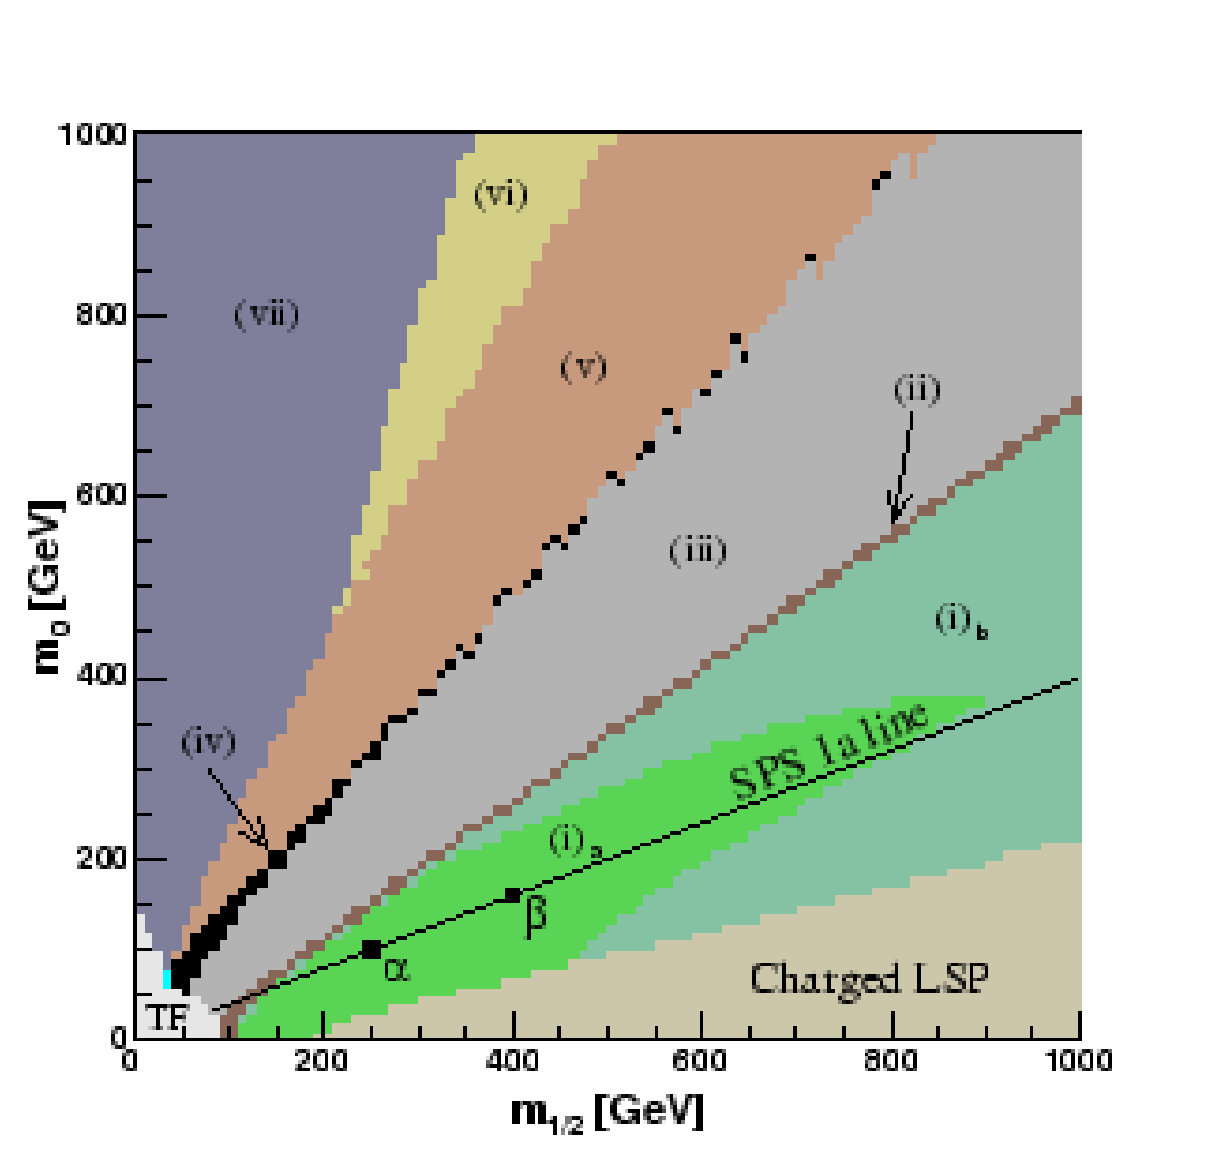
\includegraphics[width=1\textwidth]{figures/susyintro/scan_sps1a.eps}
	\caption{ }
	\label{fig:mSUGRA_decay_spectrum_a}
\end{subfigure}
\begin{subfigure}[b]{0.4\textwidth}
	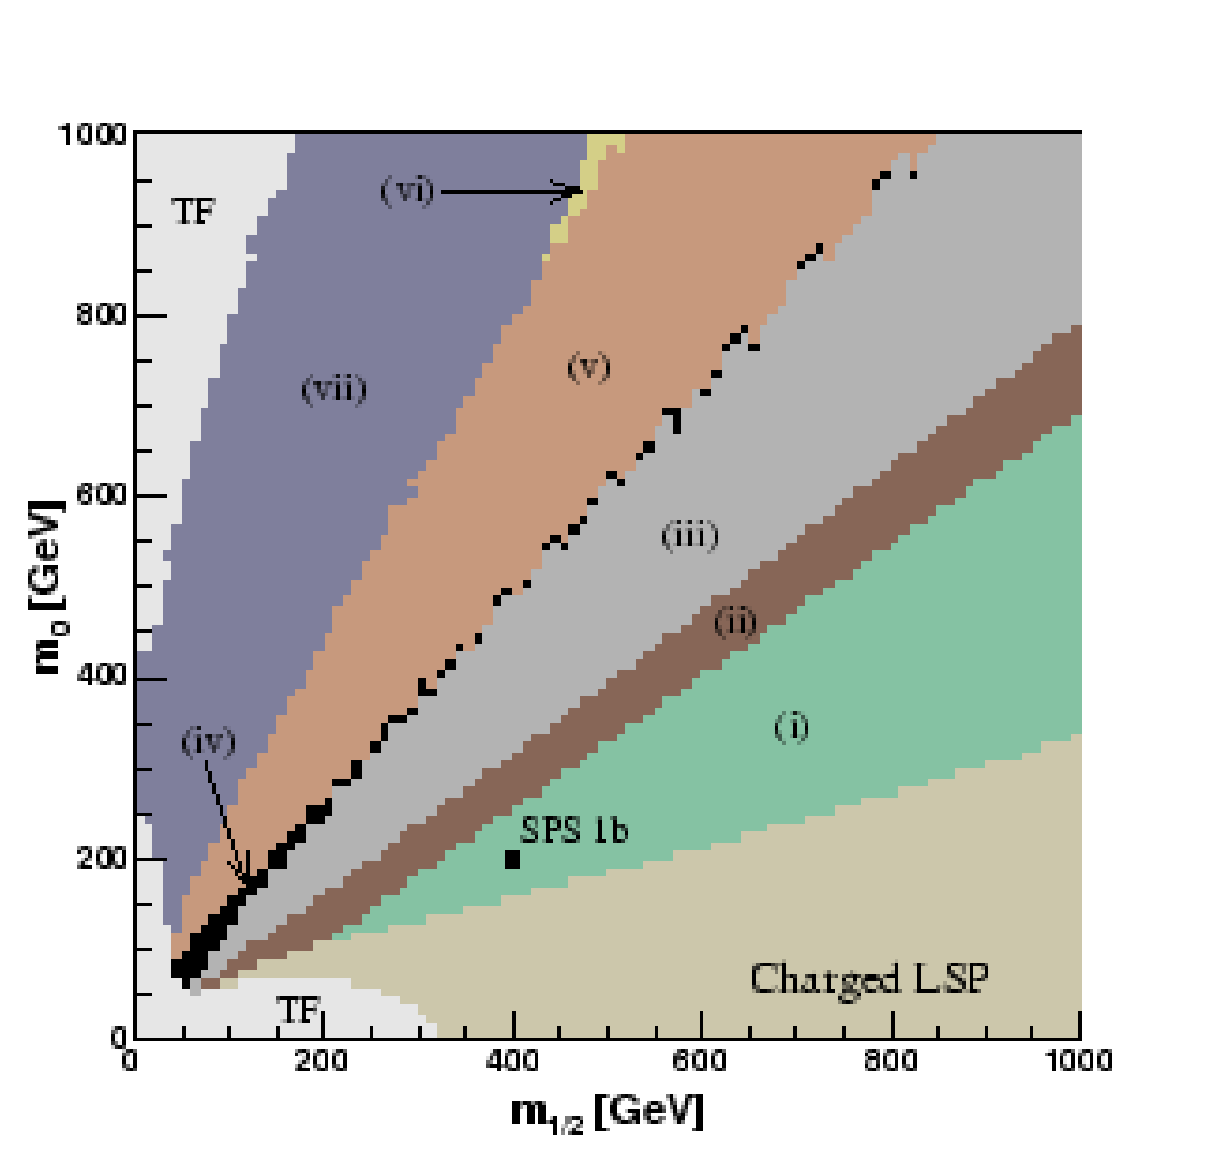
\includegraphics[width=1\textwidth]{figures/susyintro/scan_sps1b.eps}
	\caption{ }
	\label{fig:mSUGRA_decay_spectrum_b}
\end{subfigure}

\begin{subfigure}[b]{0.4\textwidth}
	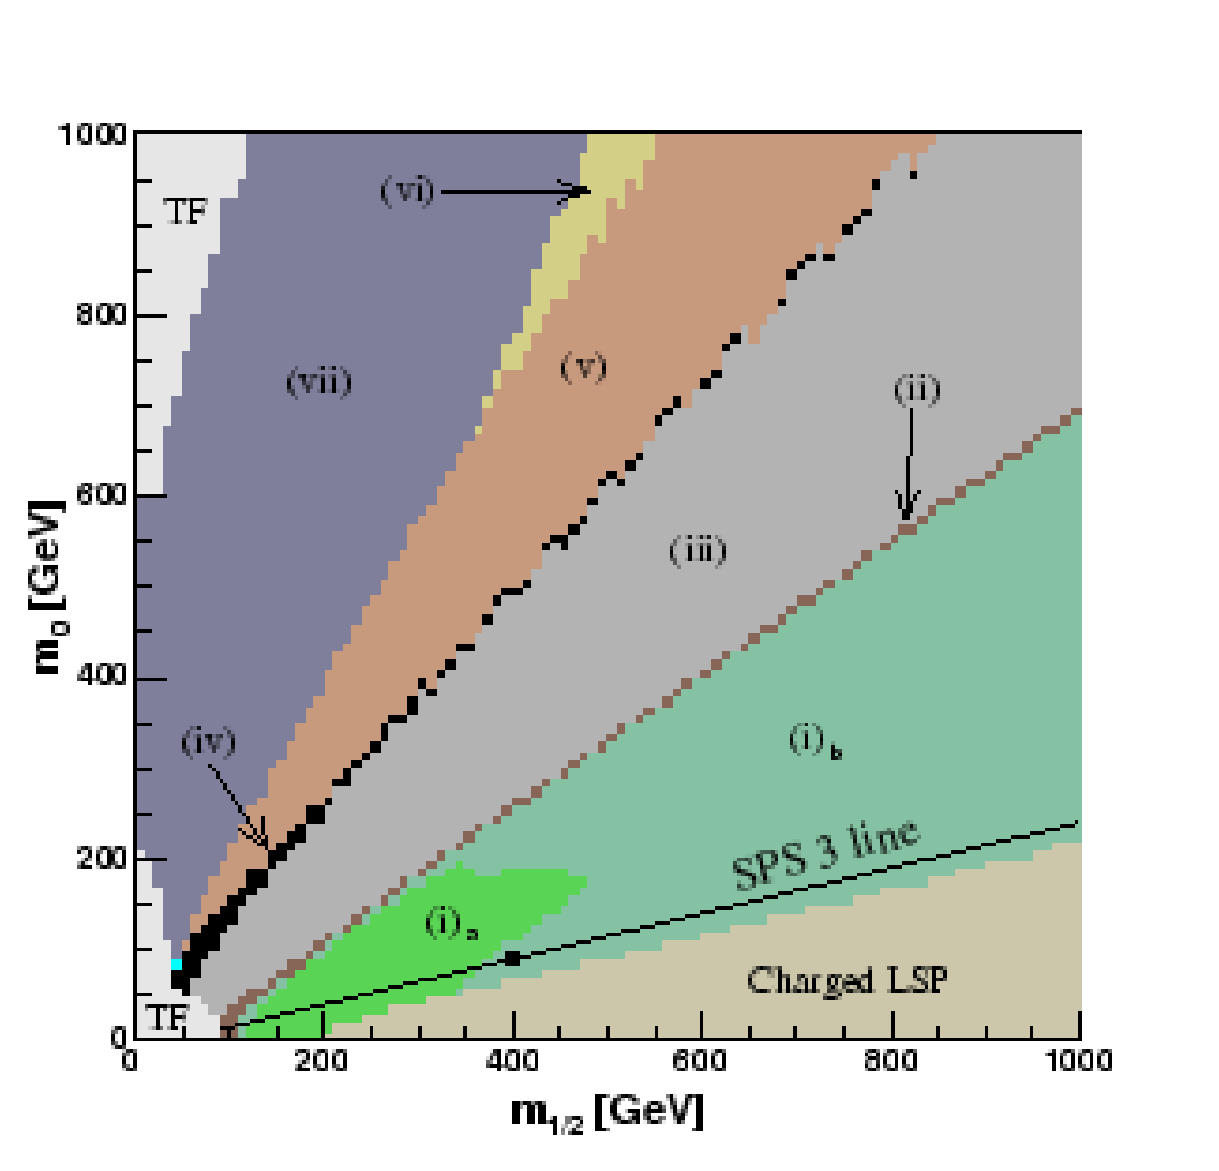
\includegraphics[width=1\textwidth]{figures/susyintro/scan_sps3.eps}
	\caption{ }
	\label{fig:mSUGRA_decay_spectrum_c}
\end{subfigure}
\begin{subfigure}[b]{0.4\textwidth}
	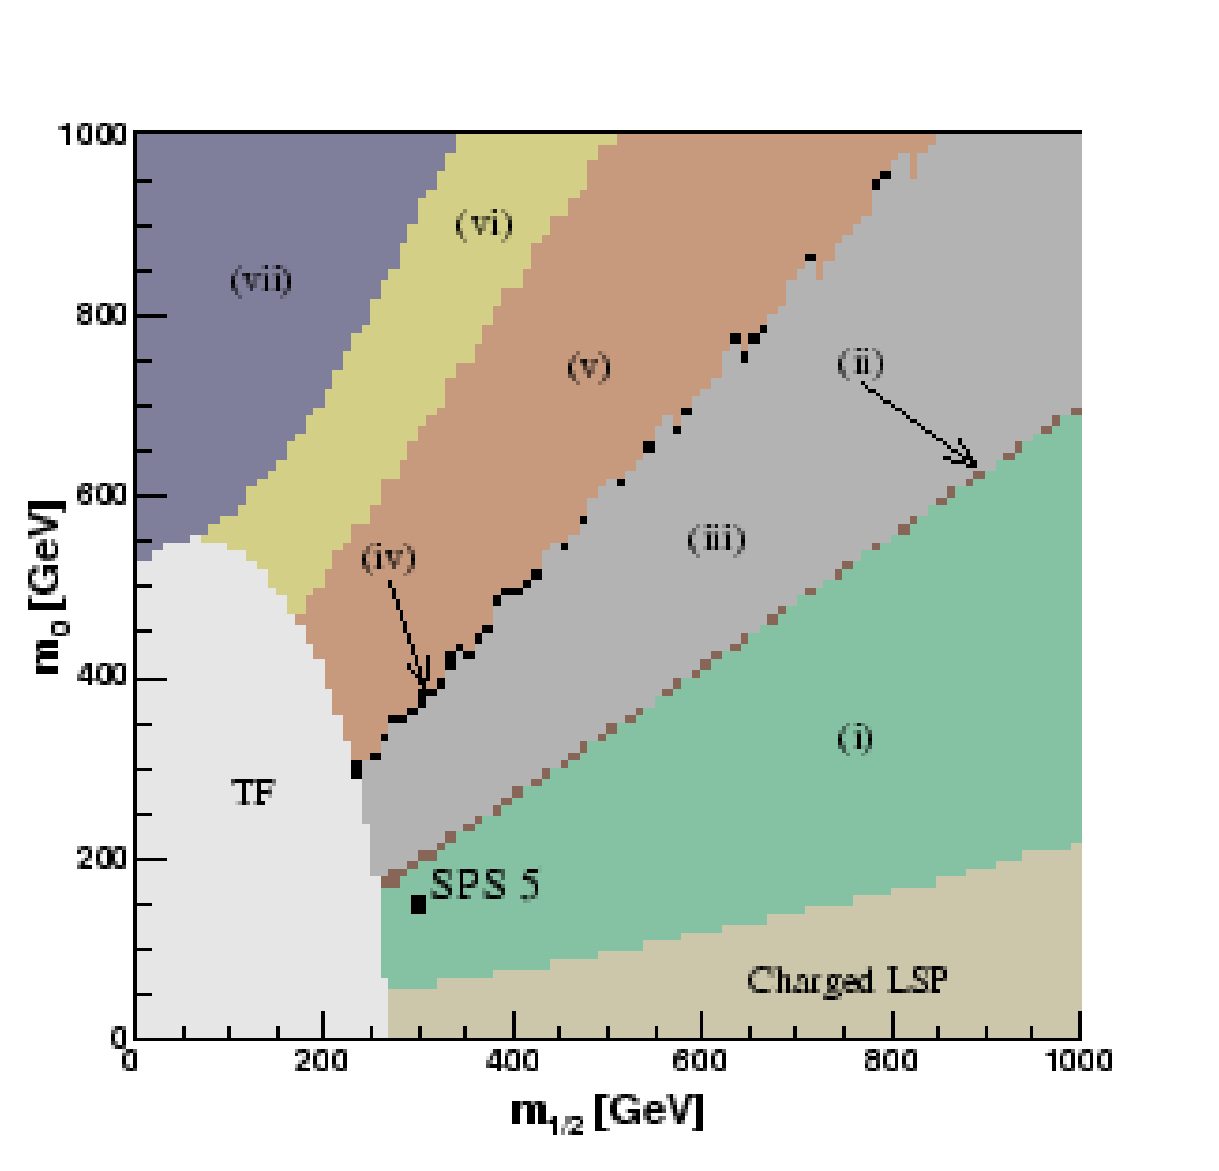
\includegraphics[width=1\textwidth]{figures/susyintro/scan_sps5.eps}
	\caption{ }
	\label{fig:mSUGRA_decay_spectrum_d}
\end{subfigure}
\caption{CMSSM mass hierarchies for different parameter choices: $A_0 = -m_0$, $\tan\beta = 10$ (a); $A_0 = 0$, $\tan\beta = 30$ (b); $A_0 = 0$, $\tan\beta = 10$ (c); and $A_0 = -1000~\mathrm{GeV}$, $\tan\beta = 5$ (d). The dark and light green areas satisfy the conditions for the decay cascade \eqref{eq:susyintrochap_cascade}. From \cite{Gjelsten:2004ki}.}
\label{fig:mSUGRA_decay_spectrum}
\end{figure}




\section{The experimental status of supersymmetry}
% {\it Include some ATLAS plots. Say something about $B_s \to \mu^+ \mu^-$ at LHCb and constraints on $\tan \beta$? Discuss mSUGRA validity? Mention more general naturalness condition?}

The search for SUSY is very actively ongoing in the LHC experiment at CERN, particularly in the ATLAS and CMS groups. Before the LHC was turned off for maintenance, it collected $\sim 20 ~\mathrm{fb}^{-1}$ of data at a centre-of-momentum energy of $\sqrt{s} = 8~\mathrm{TeV}$. No significant excesses of events that could indicate the existence of SUSY have so far been observed. At the time of writing, the LHC has begun circulating beams in preparation for Run II, which will use a centre-of-momentum energy of $\sqrt{s} = 13~\mathrm{TeV}$, and is expected to record $\sim 300 ~\mathrm{fb}^{-1}$ of data during the next ten years. In an even longer perspective, it is hoped that the machine will recieve an upgrade to the {\it high luminosity LHC}, which brings the total expected integrated luminosity up to $3000~\mathrm{fb}^{-1}$. 

The discovery of a Higgs boson with $m_h = 125.09\pm 0.21\, (\rm{stat.})\pm 0.11\, (\rm{syst.}) ~\rm{GeV}$ \cite{Aad:2015zhl} has implications for SUSY. If we assume that it is the light Higgs of SUSY, eqs.\ (\ref{eq:mssm_higgs_masses1}--\ref{eq:mssm_higgs_masses2}) puts restrictions on the combinations of the parameters $|\mu|$, $\tan\beta$ and $m^2_{H_{u/d}}$.

Figure \ref{fig:ATLAS_mSUGRA} shows a plot of the search for SUSY by ATLAS in the CMSSM model. The plot shows the $(m_0,m_{1/2})$ plane for fixed values of $\tan\beta = 30$, $A_0 = -2m_0$ and $\mu>0$. The various coloured lines indicate the lower bound for the parameter combination at 95 \% confidence level in different searches. More specifically, the solid line for each colour is the exclusion limit obtained from analysis of the collision data, while the dashed line is the theoretical exclusion limit one would expect from the Standard Model. We see that for low values of $m_0$, the searches for events with several jets and no leptons put the largest limits on the $m_{1/2}$ parameter (because a light gluino would have a large cross-section, and often decay to jets).
\begin{figure}[hbt]
	\centering
	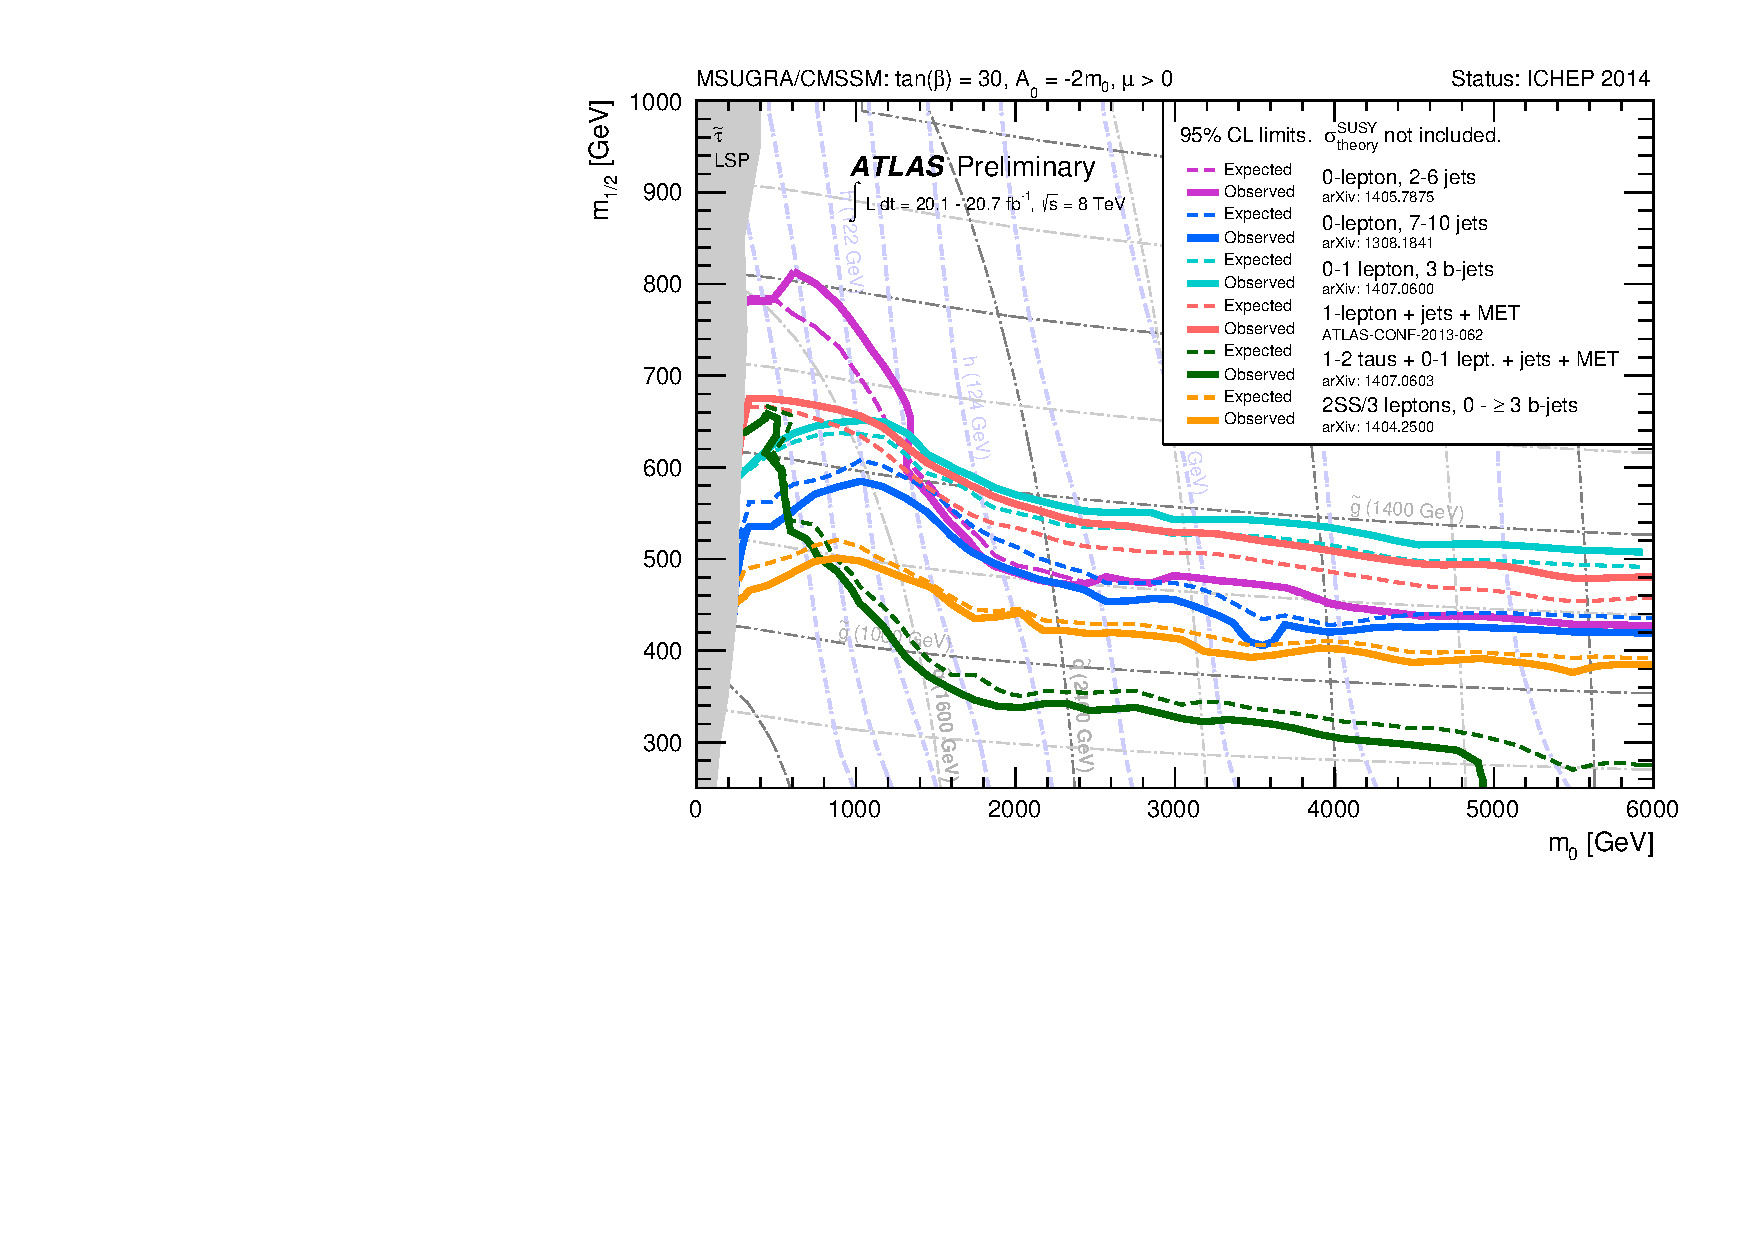
\includegraphics[width=0.9\textwidth]{figures/susyintro/ATLAS_SUSY_MSUGRA.pdf}
	\caption{CMSSM limits from ATLAS per february 2015. }
	\label{fig:ATLAS_mSUGRA}
\end{figure}

Figure \ref{fig:ATLAS_neutralinogluino} shows the same kinds of exclusion limit, but in the $(m_{\tilde q/\tilde g}, m_{\tilde \chi_1^0})$ plane. These searches assume the mass hierarchy $m_{\tilde q/\tilde g} > m_{\tilde \chi_2^0} > m_{\tilde l} > m_{\tilde \chi_1^0}$. The events considered in this analysis are required to have two (a) and four (b) jets, respectively, where none of the jets have been tagged as $b$-jets. Additionally, there must be two leptons of opposite sign and same flavour, which are not allowed to have an invariant mass between them that is compatible with a $Z$ boson decaying. Also, there must be a significant amount $(> 200 ~\mathrm{GeV})$ of missing transverse energy.
\begin{figure}[hbt]
\centering
\begin{subfigure}[b]{0.45\textwidth}
	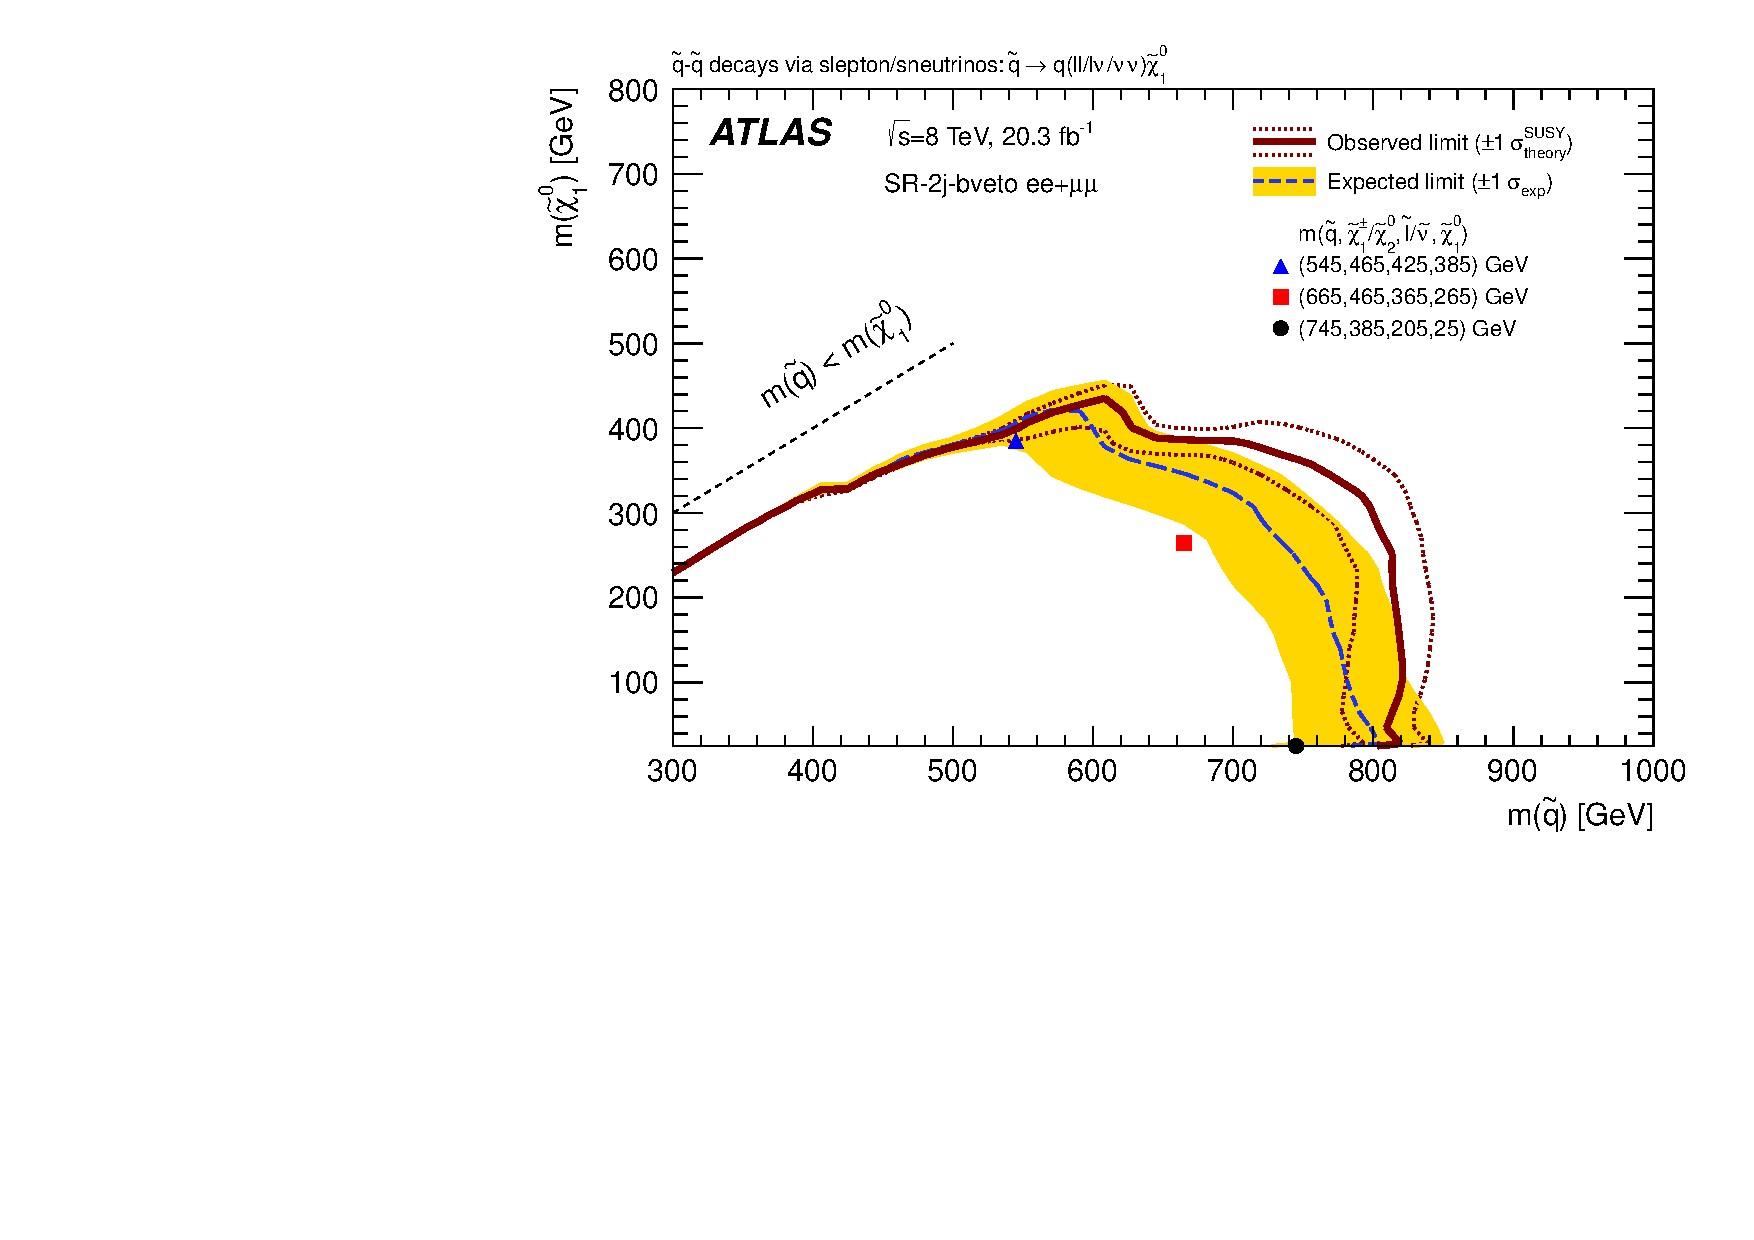
\includegraphics[width=\textwidth]{figures/susyintro/Edge_wband1_wfixSigXSecband1_showcms0_EdgeAnalysisUnblindXsec_SR2jSF.pdf}
	\caption{ }
	\label{fig:ATLAS_neutralinogluino_a}
\end{subfigure}
\begin{subfigure}[b]{0.45\textwidth}
	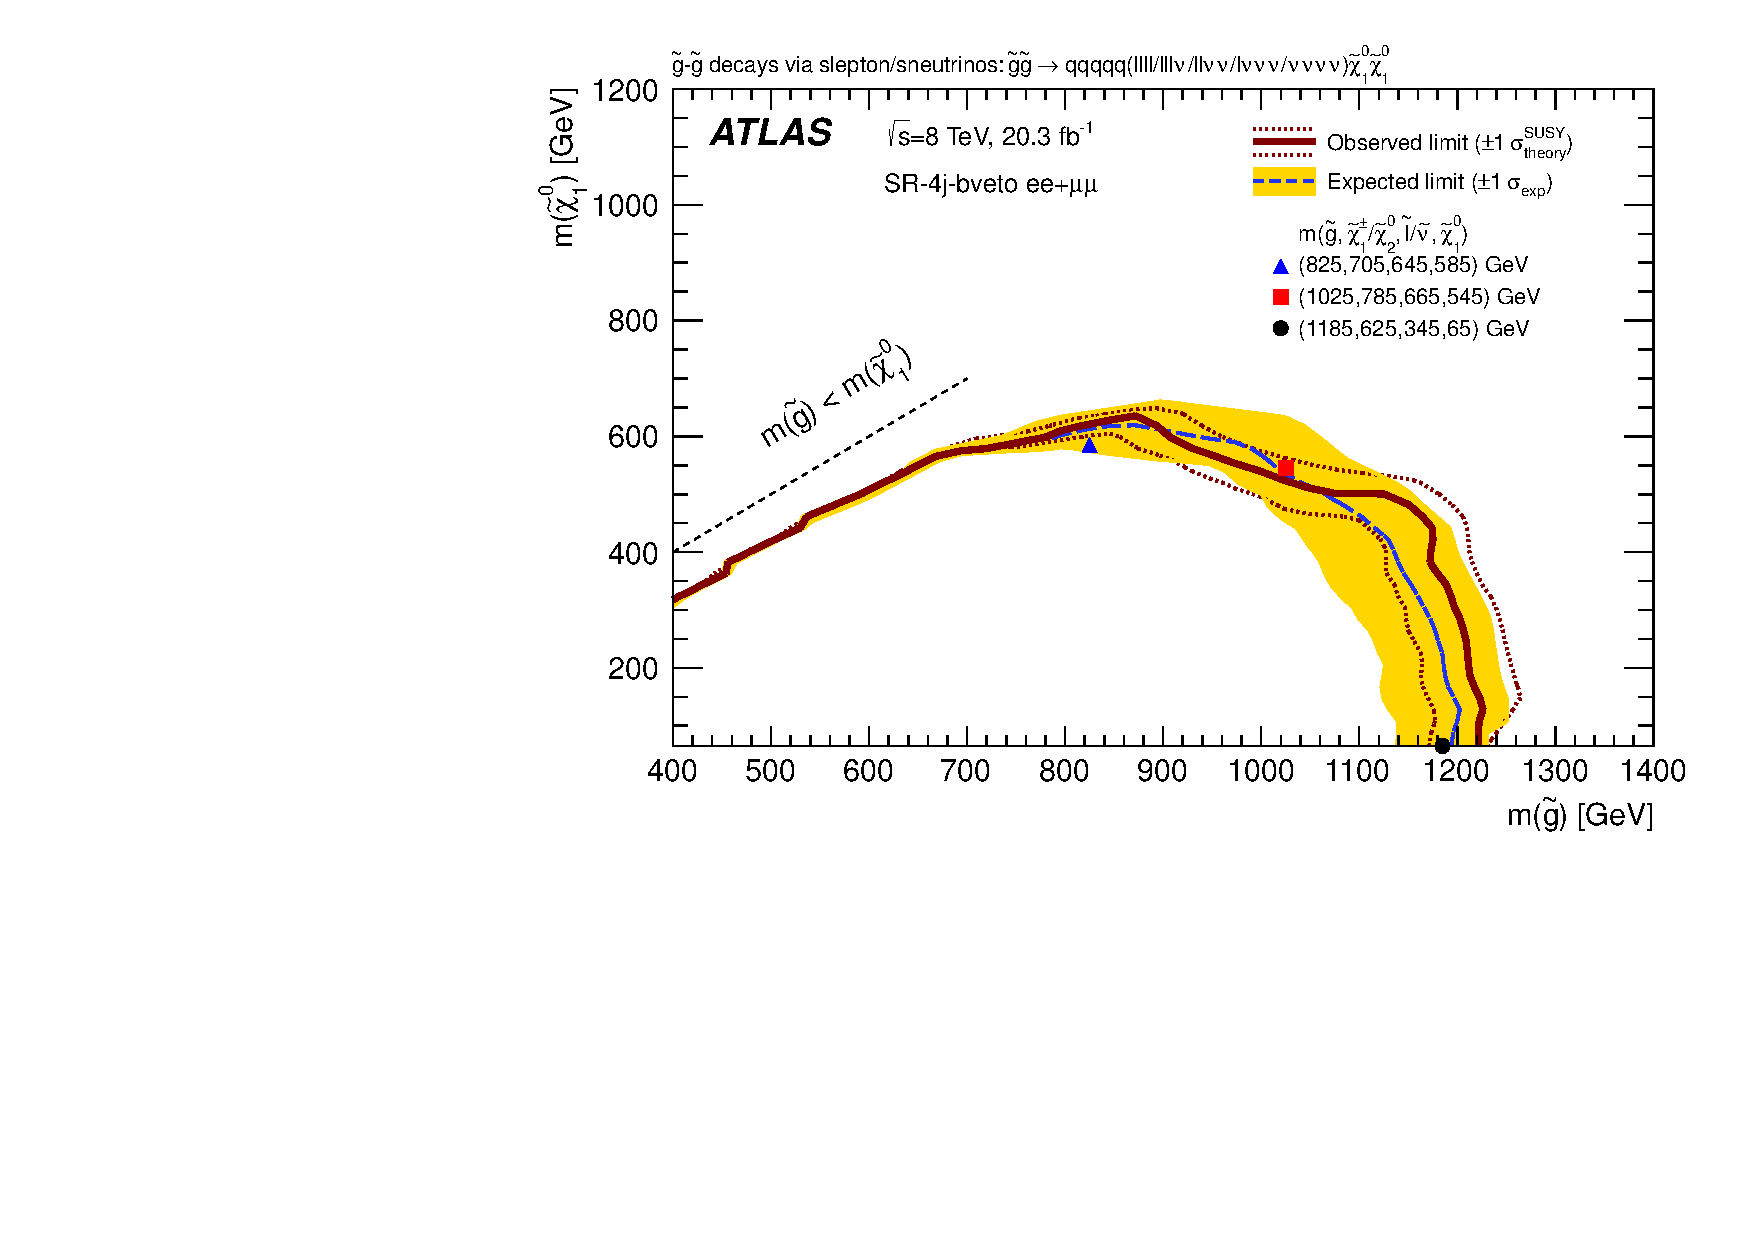
\includegraphics[width=\textwidth]{figures/susyintro/Edge_wband1_wfixSigXSecband1_showcms0_EdgeAnalysisUnblindXsec_SR4jSF.pdf}
	\caption{ }
	\label{fig:ATLAS_neutralinogluino_b}
\end{subfigure}
\caption{Limits on $\tilde q$ (a) and $\tilde g$ (b) versus $\tilde \chi_1^0$ mass in events with least two (a) or four (b) jets (none of them $b$-jets), respectively, and a same-flavour dilepton pair. From ATLAS per march 2015.}
\label{fig:ATLAS_neutralinogluino}
\end{figure}

Referring back to fig.\ \ref{fig:mSUGRA_decay_spectrum}, we see that the bright green region, where the chain hierarchy is present with a sizeable branching fraction, favours low values for $m_0$ and $m_{1/2}$. Comparing to the experimental constraints of figure \ref{fig:ATLAS_mSUGRA}, we see that much of these parts of the parameter space are ruled out. The top left region, where $m_{1/2} \gtrsim 800~\mathrm{GeV}$ and $1000 ~\mathrm{GeV} \gtrsim m_0 \gtrsim 400 ~\mathrm{GeV}$, is compatible with the green areas of fig.\ \ref{fig:mSUGRA_decay_spectrum} and is not ruled out by the ATLAS limits themselves, but it corresponds to a Higgs mass $m_h \lesssim 123 ~\mathrm{GeV}$, which is excluded. Large values of $m_0$ and $m_{1/2}$ are needed to evade the experimental constraints. All the bright green regions, where the chain has large branching, seem to be excluded. There is, however, also a question of what values are chosen for $A_0$ and $\tan\beta$, since the searches in fig.\ \ref{fig:ATLAS_mSUGRA} assume one specific choice. 

As a benchmark for the expected chain event yield, we have calculated the expected number of events in the parameter point $m_0 = 800 ~\mathrm{GeV}$, $m_{1/2} = 400 ~\mathrm{GeV}$, $A_0 = -800~\mathrm{GeV}$, $\tan\beta = 10$, $\mu>0$ for LHC Run II. This is the lowest $m_0-m_{1/2}$ combination that is not excluded by fig.\ \ref{fig:ATLAS_mSUGRA} and at the same time provides the conditions needed for the chain --- but it {\it is} excluded by the Higgs mass constraint, and we only include it for purposes of illustration. We calculate sparticle masses and branching fractions using {\tt SoftSUSY} v.\ 3.4.1 \cite{Allanach:2001kg} and squark and gluino cross-sections for 13 TeV LHC using {\tt NLL-fast} v.\ 3.0 \cite{Beenakker:1996ch,Kulesza:2008jb,Kulesza:2009kq,Beenakker:2009ha,Beenakker:2011fu,Beenakker:1997ut,Beenakker:2010nq}. Assuming an integrated luminosity of $3000~\mathrm{fb}^{-1}$ for a high-luminosity upgraded LHC\footnote{If the high-luminosity upgrade of the LHC is carried out, it will probably take data at $\sqrt{s}=14~\mathrm{TeV}$. There is, however, no complete implementation of {\tt NLL-fast} for $14 ~\mathrm{TeV}$.}, we find an expectation of 3 events. 

To evade the experimental constraints of the Higgs mass and ATLAS SUSY searches, and at the same time keep the conditions needed for the chain as given in fig.\ \ref{fig:mSUGRA_decay_spectrum}, it appears that both the $m_0$ and $m_{1/2}$ parameters need to be pushed to or above 1000 GeV. Increasing the masses reduces the production cross-section, which means that even an expectation of 3 events may be optimistic. Thus, it seems that the golden decay chain is difficult to realize in the CMSSM.

However, by loosening some of the constraining assumptions of the CMSSM, such as the soft mass unification at a high scale, more general parametrizations of SUSY may be defined. The failure of the LHC to find SUSY has prompted a large interest in studies of these more general models, often termed ``Natural SUSY'' since the main guiding principle is to avoid the need for fine-tuning, such as the {\it Little Hierarchy Problem} of the Higgs mass discussed in appendix \ref{appendix:higgs_mass_loop_correction}. In these models, the squark and gluino masses may decouple, pushing {\it e.g.}\ the gluino to high mass while retaining light squarks. This may evade the experimental constraints such as the Higgs mass, and still give high cross-sections for squark production to initiate the chain.

% There are also other experimental signatures that can be used to set limits on SUSY parameters. One notable example is the branching fraction for the decay $B_s \to \mu^+ \mu^-$, which has a would-be SUSY contribution which is heavily dependent on $\tan\beta$. So far, analyses by the CMS and LHCb groups \cite{CMS:2014xfa} have found results which match the predictions of the Standard Model to high precision, thus placing stringent limits on any non-Standard Model contributions. \marginpar{Remove this paragraph?}


















%%%%%%%%%%%%%%%%%%%%%%%%%%%%%%%%%%%%%%%%%%%%%%%%%%%%%%%%%%%%%%%%%%%%%%%%%%%
\chapter{Determination of SUSY particle masses from cascade decays}%%%%%%%%
%%%%%%%%%%%%%%%%%%%%%%%%%%%%%%%%%%%%%%%%%%%%%%%%%%%%%%%%%%%%%%%%%%%%%%%%%%%
\label{ch:introducing_the_method}




\section{The problem}
Consider an LHC event where two chains of the form
\begin{align}
	\tilde{q} \to q + \tilde{\chi}_2^0, \, \tilde{\chi}_2^0 \to l^{\pm} + \tilde{l}^\mp, \, \tilde{l}^\mp \to l^\mp + \tilde{\chi}_1^0\label{eq:goldencascade}
\end{align}
are present. Combined, the measurable particles in the two chains are the two quarks and four leptons, where the lepton pairs are opposite-sign same-flavour. The LSPs escape detection, but the sum of their transverse momenta can be measured as the missing $p_T$. The quantities of interest, however, are the masses of the supersymmetric particles, $m_{\tilde{q}}, m_{\tilde{\chi}_2^0}, m_{\tilde{l}}$ and $m_{\tilde{\chi}_1^0}$. (Potentially with several values for the squarks and sleptons if they differ in generation and/or chirality between the sides.) These are not directly measurable, but the kinematics of the problem depend on them. 

Many methods have been investigated for the purpose of measuring supersymmetric masses \cite{Barr:2010zj}. One well known example is the end-point method \cite{1126-6708-2000-09-004}. We measure {\it e.g.}\ the dilepton invariant mass in the process \eqref{eq:goldencascade}. The distribution of the dilepton invariant mass can be shown to form a right triangle where the maximal value is given by
\begin{align}
	(m_{ll}^\mathrm{max})^2 = \frac{ \left( m^2_{\tilde{\chi}_2^0} - m^2_{\tilde{l}} \right) \left( m^2_{\tilde{l}} - m^2_{\tilde{\chi}_1^0} \right)}{m^2_{\tilde{l}}}, \label{eq:invariant_mass_endpoint}
\end{align}
thus constraining $m_{\tilde{\chi}_2^0}$, $m_{\tilde{l}}$ and $m_{\tilde{\chi}_1^0}$. Similar constraints may be obtained for the three other visible particle combinations, giving four equations with four unknowns. This method is very dependent on statistics, since each measured event only contributes one point to the distribution. A large number of events is required to get a reliable value. However, the number of events contributing to the measurement is also much larger, since each side of the decay chain contribute individually, thus making use of events with leptons on one side only as well.



\section{Webber's method}
Webber \cite{Webber:2009vm} suggests a different method, where all available kinematical info from every event is used. Consider the general decay tree in fig. \ref{fig:decaytree}. We assume that we have an event with two such chains, but not necessarily with identical particles in the two. We will distinguish the two chains by referring to them as the ``first'' and ``second'' one, although the assignment is arbitrary.
\begin{figure}[hbt]
\centering
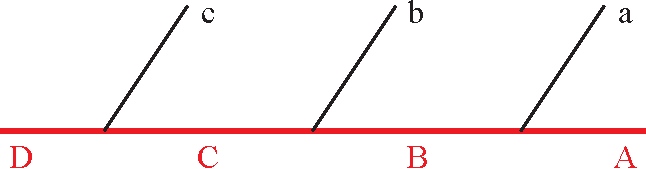
\includegraphics[scale=0.7]{figures/fig-chain.pdf} % Stolen!
\caption{Decay topology, from \cite{Miller:2005zp}.}
\label{fig:decaytree}
\end{figure}
Assuming that the decaying particles are on-shell, the four-momenta in the first chain should satisfy
\begin{align}
	(p_c + p_b + p_a + p_A)^2 &= M_D^2,\nonumber \\
	(p_b + p_a + p_A)^2 &= M_C^2,\nonumber \\
	(p_a + p_A)^2 &= M_B^2,\label{eq:constraints}\\
	p_A^2 &= M_A^2.\nonumber
\end{align}
The first three equations give three linear constraints on the invisible four-momentum $p_A$:
\begin{align}
	-2p_c\cdot p_A &= M_C^2 - M_D^2 + 2p_c\cdot p_b + 2p_c \cdot p_a + m_c^2 \equiv S_1,\nonumber \\
	-2p_b\cdot p_A &= M_B^2 - M_C^2 + 2p_b\cdot p_a + m_b^2 \equiv S_2,\\
	-2p_a\cdot p_A &= M_A^2 - M_B^2 + m_a^2 \equiv S_3. \nonumber
\end{align}
Equivalently the second chain (with primed indices) gets the constraints
\begin{align}
	-2p_{c'}\cdot p_{A'} &= M_{C'}^2 - M_{D'}^2 + 2p_{c'}\cdot p_{b'} + 2p_{c'} \cdot p_{a'} + m_{c'}^2 \equiv S_5,\nonumber \\ 
	-2p_{b'}\cdot p_{A'} &= M_{B'}^2 - M_{C'}^2 + 2p_{b'}\cdot p_{a'} + m_{b'}^2 \equiv S_6,\\
	-2p_{a'}\cdot p_{A'} &= M_{A'}^2 - M_{B'}^2 + m_{a'}^2 \equiv S_7.\nonumber
\end{align}
In addition we have the transverse momentum constraints
\begin{align}
	p_A^x + p_{A'}^x &= p_\mathrm{miss}^x \equiv S_4, \label{eq:Svec_orig} \\
	p_A^y + p_{A'}^y &= p_\mathrm{miss}^y \equiv S_8. \nonumber
\end{align}

The vector $\mathbf{S} = (S_1, S_2, ...)$ thus depends on the eight unknown masses 
\begin{align}
	\mathbf{M} = (M_D^2, M_C^2, M_B^2, M_{A'}^2, M_{D'}^2, M_{C'}^2, M_{B'}^2, M_{A'}^2)
\end{align}
and the visible momenta which in principle are measurable. We define a vector containing the four-momenta of the invisible final state particles as
\begin{align}
	\mathbf{P} = (p_A^x, p_A^y, p_A^z, E_A, p_{A'}^x, p_{A'}^y, p_{A'}^z, E_{A'}). \label{eq:Pvec}
\end{align}
We then have
\begin{align}
	\mathbf{A}\mathbf{P} = \mathbf{S},\label{eq:APS}
\end{align}
where
\begin{align}
	\mathbf{A} = 2 \begin{pmatrix}
						p_c^x & p_c^y & p_c^z & -E_c & 0 & 0 & 0 & 0 \\
						p_b^x & p_b^y & p_b^z & -E_b & 0 & 0 & 0 & 0 \\
						p_a^x & p_a^y & p_a^z & -E_a & 0 & 0 & 0 & 0 \\
						1/2 & 0 & 0 & 0 & 1/2 & 0 & 0 & 0\\
						0 & 0 & 0 & 0 & p_{c'}^x & p_{c'}^y & p_{c'}^z & -E_{c'} \\
						0 & 0 & 0 & 0 & p_{b'}^x & p_{b'}^y & p_{b'}^z & -E_{b'} \\
						0 & 0 & 0 & 0 & p_{a'}^x & p_{a'}^y & p_{a'}^z & -E_{a'} \\
						0 & 1/2 & 0 & 0 & 0 & 1/2 & 0 & 0
					\end{pmatrix}. \label{eq:Amatrix_orig}
\end{align}
Furthermore, $\mathbf{S}$ may be written as 
\begin{align}
	\mathbf{S} = \mathbf{B} \mathbf{M} + \mathbf{C},\label{eq:SBMC}
\end{align}
where
\begin{align}
	\mathbf{B} = \begin{pmatrix}
					-1 & 1 & 0 & 0 & 0 & 0 & 0 & 0 \\
					0 & -1 & 1 & 0 & 0 & 0 & 0 & 0 \\
					0 & 0 & -1 & 1 & 0 & 0 & 0 & 0 \\
					0 & 0 & 0 & 0 & 0 & 0 & 0 & 0 \\
					0 & 0 & 0 & 0 & -1 & 1 & 0 & 0 \\
					0 & 0 & 0 & 0 & 0 & -1 & 1 & 0 \\
					0 & 0 & 0 & 0 & 0 & 0 & -1 & 1 \\
					0 & 0 & 0 & 0 & 0 & 0 & 0 & 0 \\
	\end{pmatrix}
\end{align}
and
\begin{align}
	\mathbf{C} = ( &2p_c \cdot p_b + 2p_c \cdot p_a + m_c^2, 2 p_2 \cdot p_3 + m_b^2, m_a^2, p_\mathrm{miss}^x, \nonumber \\ 
				   &2p_{c'}\cdot p_{b'} + 2 p_{c'} \cdot p_{a'} + m_{c'}^2, 2 p_{b'} \cdot p_{a'} + m_{b'}^2, m_{a'}^2, p_\mathrm{miss}^y )
\end{align}
With all this, the solution for the invisible four-momenta, given the unknown masses, is 
\begin{align}
	\mathbf{P} = \mathbf{A}^{-1} \mathbf{S} = \mathbf{D} \mathbf{M} + \mathbf{E},
\end{align}
where $\mathbf{D} = \mathbf{A}^{-1}\mathbf{B}$ and $\mathbf{E} = \mathbf{A}^{-1}\mathbf{C}$.

The matrix $\mathbf{D}$ and vector $\mathbf{E}$ contain only measurable quantities, hence they only need to be calculated once for every event. For the true value of the unknown masses $\mathbf{M}$, the system should satisfy the on-shell conditions
\begin{align}
	p_{A}^2 &= P_4^2 - P_1 ^2 - P_2^2 - P_3^2 = M_{A}^2, \nonumber\\
	p_{A'}^2 &= P_8^2 - P_5 ^2 - P_6^2 - P_7^2 = M_{A'}^2.
\end{align}
So by calculating $\mathbf{D}_n$ and $\mathbf{E}_n$ for each event $n$, and making a {\it hypothesis} $\mathbf{M}$ for the unknown masses, we can measure the goodness of fit for our hypothesis by the quantity
\begin{align}
	\xi^2(\mathbf{M}) = \sum_n \left[(p_{A}^2)_n - M_A^2\right]^2 + \left[(p_{A'}^2)_n - M_{A'}^2\right]^2. \label{eq:xisquared}
\end{align}
Note that this quantity measures the goodness-of-fit of all the unknown masses equally, since it follows from the constraint equations \eqref{eq:constraints} that {\it e.g.}
\begin{align}
	(p_B^2)_n - M_B^2 &= (p_a + p_A)_n^2 - M_B^2 = \nonumber\\
				  &= (p_a^2)_n + (p_A^2)_n + 2p_a\cdot p_A - M_B^2\nonumber\\
				  &= (p_a^2)_n + (p_A^2)_n - M_A^2 + M_B^2 - m_a^2 - M_B^2\\
				  &= (p_A^2)_n - M_A^2.\nonumber
\end{align}

For each event there are eight constraining equations. There are eight unknowns from the masses plus six from the unknown LSP momenta (using the on-shell constraint on the LSPs). The system is thus underconstrained, with six free parameters. The point of the method is to minimize $\xi^2$ as a function of $\mathbf{M}$. This is generally an eight-dimensional minimization problem with a potentially very complicated function, and thus not easy to solve. However, in the case of identical chains, it reduces to a much more handleable four-dimensional one which one could hope could be solved. In this case the number of free parameters reduces from six to two. The condition of identical chains can often be satisfied by a combination of vetoing ({\it e.g.} b-jets) and assuming small mass splittings between different generations, thus approximating their masses as equal. As was discussed in section \ref{sec:cmssm}, this is a realistic assumption in many SUSY scenarios.

\section{Two technical modifications}\label{sec:dimension_fixing}
For the method to be applicable, the matrix $\mathbf{A}$ must be invertible. A matrix is invertible if its determinant is non-zero. However, the matrix as it stands in \eqref{eq:Amatrix_orig}, is technically ill-defined for inversion since not all rows have the same units. The rows 4 and 8, corresponding to the components 4 and 8 of the vector $\mathbf{S}$ \eqref{eq:Svec_orig}, have no dimension, while the other rows have dimension $[\mathrm{mass}]^1$. This is reflected in the components of $\mathbf{S}$, which all except 4 and 8 have dimension $[\mathrm{mass}]^2$. This means both that the magnitude of the determinant is sensitive to the choice of mass scale (since some rows have non-zero dimension) and that it does not scale properly for numerical calculations (since not all rows have the same dimension). This is something that Webber does not comment on (and the method still in principle works), but we make some minor reformulations of the method in order to amend both problems.

For the first, we redefine $S_4$ and $S_8$ to be 
\begin{align}
	S_4 &\equiv (p_A^x + p_{A'}^x)^2 = (p_\mathrm{miss}^x)^2, \label{eq:Svec_modified} \\
	S_8 &\equiv (p_A^y + p_{A'}^y)^2 = (p_\mathrm{miss}^y)^2. \nonumber
\end{align}
We do not wish to redefine $\mathbf{P}$ \eqref{eq:Pvec}, so to keep the relationship $\mathbf{S} = \mathbf{A}\mathbf{P}$ we modify rows 4 and 8 of $\mathbf{A}$ to
\begin{align}
	\mathbf{A}_4 &= (p_\mathrm{miss}^x, 0, 0, 0, p_\mathrm{miss}^x, 0, 0, 0),\\
	\mathbf{A}_8 &= (0, p_\mathrm{miss}^y, 0, 0, 0, p_\mathrm{miss}^y, 0, 0),\nonumber
\end{align}
such that $\mathbf{A}$ now is
\begin{align}
	\mathbf{A} = 2 \begin{pmatrix}
						p_c^x & p_c^y & p_c^z & -E_c & 0 & 0 & 0 & 0 \\
						p_b^x & p_b^y & p_b^z & -E_b & 0 & 0 & 0 & 0 \\
						p_a^x & p_a^y & p_a^z & -E_a & 0 & 0 & 0 & 0 \\
						p_\mathrm{miss}^x/2 & 0 & 0 & 0 & p_\mathrm{miss}^x/2 & 0 & 0 & 0\\
						0 & 0 & 0 & 0 & p_{c'}^x & p_{c'}^y & p_{c'}^z & -E_{c'} \\
						0 & 0 & 0 & 0 & p_{b'}^x & p_{b'}^y & p_{b'}^z & -E_{b'} \\
						0 & 0 & 0 & 0 & p_{a'}^x & p_{a'}^y & p_{a'}^z & -E_{a'} \\
						0 & p_\mathrm{miss}^y/2 & 0 & 0 & 0 & p_\mathrm{miss}^y/2 & 0 & 0
					\end{pmatrix}. \label{eq:Amatrix_modified}
\end{align}

This redefinition does not alter the solvability of the problem, since the only information lost in $\mathbf{S}$ is the sign of $p_\mathrm{miss}^i$ which is kept in $\mathbf{A}$ instead. Also it keeps the essential feature that $\mathbf{A}$ only contains measured quantities, so that it can be inverted prior to making a mass hypothesis. The redefinition of $\mathbf{S}$ means we also have to modify $\mathbf{C}$ to keep the relationship $\mathbf{S} = \mathbf{B} \mathbf{M} + \mathbf{C}$ (from eq.\ \eqref{eq:SBMC}). We thus make the same redefinitions here, {\it i.e.}
\begin{align}
	C_4 &\equiv (p_\mathrm{miss}^x)^2, \label{eq:Cvec_modified} \\
	C_8 &\equiv (p_\mathrm{miss}^y)^2. \nonumber
\end{align}

The other issue is to make the numerical problem dimensionless. All elements of $\mathbf{A}$ and $\mathbf{P}$ now have mass dimension 1, while all elements of $\mathbf{S}$, and thus $\mathbf{M}$ and $\mathbf{C}$, have dimension 2. We are free to multiply both sides of eq.\ \eqref{eq:APS} by some normalization mass $M_\mathrm{norm}$ squared,
\begin{align}
	\frac{1}{M_\mathrm{norm}^2} \mathbf{A}\mathbf{P} = \frac{1}{M_\mathrm{norm}^2} \mathbf{S},
\end{align}
and we choose to take it into the matrix and vectors such that they all become dimensionless, {\it i.e.}\ we modify
\begin{align}
	\mathbf{\hat A} = \frac{1}{M_\mathrm{norm}}\mathbf{A},\nonumber \\
	\mathbf{\hat P} = \frac{1}{M_\mathrm{norm}}\mathbf{P},\label{eq:vectors_normalized}\\
	\mathbf{\hat S} = \frac{1}{M_\mathrm{norm}^2}\mathbf{S},\nonumber 
\end{align}
thus modifying $\mathbf{M}$ and $\mathbf{C}$ in the same way as $\mathbf{S}$ to comply with eq.\ \eqref{eq:SBMC}. We also modify the fitting function $\xi^2$ accordingly, so that it becomes
\begin{align}
	\xi^2(\mathbf{M}) = \sum_n \left[(\hat p_{A}^2)_n - \frac{M_A^2}{M_\mathrm{norm}^2}\right]^2 + \left[(\hat p_{A'}^2)_n - \frac{M_{A'}^2}{M_\mathrm{norm}^2}\right]^2.\label{eq:xisquared_modified}
\end{align}

To obtain numbers of order one, which is optimal for numerical purposes, we should pick a mass of the relevant scale for the problem. This is not something that is known {\it a priori}, since it depends on the supersymmetric masses that we are trying to determine. We might be tempted to use something based on the measured momenta, but this is a bad idea since it would mean weighting different events differently. We choose the normalization constant
\begin{align}
	M_\mathrm{norm} = 100 ~\mathrm{GeV},
\end{align}
the same order of magnitude as we expect for the supersymmetric masses ($\sim$ electroweak scale). 

We have made thorough checks that this formulation and the original one produce identical results within numerical accuracy, so that indeed the formulations are equivalent.









\section{Taking account of combinatorics}
\label{sec:combinatorics}
In a real detector event, the ordering of the quarks and leptons in and between chains is not known --- all we have are the measured particle types and their momenta. We must take this into account when applying the method to Monte Carlo simulated datasets. Webber does this by evaluating all possible combinations in each event at each mass point and selecting the combination which gives the lowest $\xi^2$ value, choosing to add this value to the sum in eq.\ \eqref{eq:xisquared_modified}. The number of possible combinations are 8 or 16, depending on whether the lepton pairs in the two chains are the same flavour or not. 

For two pairs of different-generation leptons, the possible orderings are (given some `base ordering' which we permute from): Switching the ordering of the leptons in the first chain; switching the ordering of the leptons in the second chain; or switching the leptons in both chains. For each of these permutations we have the option to switch the two quarks, so the total number of combinations is 8. In the case of identical leptons, we may additionally interchange leptons between the chains ---but this only increases the total combinations by a factor of 2 because the same-chain leptons must have opposite charge.

Note that in order to switch the ordering of leptons within the same chain, all we need to do is permute the rows of the matrix $\mathbf{A}$. The vector $\mathbf{C}$ is invariant as long as the same-chain leptons have the same mass. When the quarks are flipped, however, or when leptons are interchanged between chains, then we must redefine $\mathbf{A}$ and $\mathbf{C}$. Webber makes a point that this property can save computer memory, since one only has to store two or four versions of the matrix and vector for each event. We have not found this to be an issue.












\section{Outline of the plan}
\marginpar{Better reformulate away from ``reproduce'', and also modify to be what I actually do}
In this thesis we wish to investigate and develop this method further. We will begin by trying to reproduce Webber's parton level results using Monte Carlo simulations. We will then add layers of realism and complexety approaching something closer to the real experimental situation, in order to investigate its full potential. In the end we will focus on well motivated scenarios that can be discovered in Run II of the LHC.  Along the way we will also make some improvements on the method.

The plan of attack is as follows:
\begin{enumerate}
	\item We begin by generating squark pairs at rest, decaying them in the chain of on-shell two-body decays given in (\ref{eq:goldencascade}). The visible decay products, quarks and leptons, are then used to reconstruct the masses. As a benchmark we investigate the precision attainable for the CMSSM parameter point SPS1a~\cite{Allanach:2002nj}, which was used by Webber. 
	\item Because of final state radiation and parton showering, as well as---to a lesser degree---sparticle widths, the particles in the decay chain will not be on-shell due to extra gluons (and photons) in the final state. We employ a more sophisticated Monte Carlo code, {\tt Herwig++}~\cite{Bahr:2008pv}  to simulate these properties. This should have an effect on the mass reconstruction since Webber's method assumes on-shell decays.
	\item	We then compare results with and without including the combinatorical issues from identifying the decay products, and we add a simple parametrised momentum smearing, based on realistic detector response, in order to simulate that the measurement of the kinematics of final-state particles is not exact. This was the level of precision employed by Webber in~\cite{Webber:2009vm}.
	\item The partons that emerge from the hadron showers will hadronize, forming a hadron jet before arriving in the detector. Measurement of the initial parton from reconstructing such jets is one of the big challenges of collider physics. We use the {\tt FastJet}~\cite{Cacciari:2011ma} program for jet reconstruction, with algorithms used in the LHC experiments, and study the effect of jet reconstruction on the mass measurement.
	\item In an analysis of real data, one would have to use selection criteria such as cuts on transverse momentum and number of jets and leptons to discriminate between signal and background events. We will apply such cut schemes to our simulated events based on expectations for 14 TeV LHC. In addition we simulate the expected largest backgrounds for a four-lepton supersymmetry search and investigate how the performance of the method is affected by the presence of background.\marginpar{Remove mention of background?}
	% \item {\bf If time} As a last step towards realism, we put the events through a fast detector simulation. 
	% \item We then investigate improvements over the original model. Webber and collaborators \cite{Nojiri:2010dk} propose combining the kinematical best-fit reconstruction with measurements of end points of invariant mass distributions.
	% \item Investigating other types of chains. Not-equal-sided? Different number of steps? Fitting a mass plane rather than points?
	% \item Finally, we look at a well motivated model taken from \cite{Allanach:2014gsa} that was constructed on the basis of a small excess seen in 8 TeV data by the CMS Collaboration~\cite{CMS:2014jfa}, which would be consistent with the decay chain in (\ref{eq:goldencascade}). We show what precission we can expect from mass measurments at 14 TeV LHC should such a scenario be realized.
\end{enumerate}






























%%%%%%%%%%%%%%%%%%%%%%%%%%%%%%%%%%%%%%%%%%%%%%%%%
\chapter{Investigating Webber's method by Monte Carlo simulations}
\label{ch:MC}
%%%%%%%%%%%%%%%%%%%%%%%%%%%%%%%%%%%%%%%%%%%%%%%%%
Webber demonstrates the aptitude of the method on a Monte Carlo generated dataset. A natural starting point for our study is to try to reproduce his results. 

\section{Collider physics}
There are several ways in which a pair of squarks can be produced in $pp$ collisions. The three main categories are: direct pair production of two squarks or a squark-antisquark pair; squark plus gluino with subsequent gluino decay to a squark; and pair production of two gluinos which both subsequently decay to squarks. The mechanism of production affects how much momentum goes into the squark, and thus the momentum of the subsequent decay chain. But our method deals mainly with the internal kinematics of the squark decay, which by Lorentz invariance is independent of squark momentum. The only variables in our analysis which explicitly depends on the overall event kinematics is the missing transverse momentum. The three different categories also affect how many hard jets are present in the event, which affects the combinatorical aspects of reconstructing the chain.

\section{Reproducing Webber's results}
Webber uses Fortran {\tt HERWIG} version 6.510 \cite{Corcella:2000bw,Moretti:2002eu} to produce events, selecting only events with two left-handed first- or second generation squarks (to limit the mass splitting), but irrespective of the hard production process. The analysis, {\it i.e.} minimization of the $\xi^2$, is performed on 100 samples of 25 events each, using the Minuit {\tt Simplex} \cite{James:1975dr} routine for minimization. He models the effects of measurement errors in a real detector by applying momentum smearing according to a gaussian distribution, and he puts a cut on the total $\xi^2$ obtained at the minimum to eliminate samples which give a bad result. His results are summarized in table 1 of \cite{Webber:2009vm}, which we for convenience show in table \ref{table:webber_original}. 
\begin{figure}[hbt]
	\centering
	\includegraphics[width=0.6\textwidth]{figures/webber_rec_table/sps1a_fits.eps} 
	\caption{Figure 2 from \cite{Webber:2009vm}, displayed here for comparison.}
	\label{fig:webber_scatter}
\end{figure}
The column $\delta p/p$ indicates the standard deviation of the gaussian smearing applied on the momenta, $\xi^2_\mathrm{max}$ indicates the cut value of the $\xi^2$, $f_\xi$ is the fraction of samples surviving the cut and $f_\mathrm{corr}$ is the fraction of events where the chosen particle combination, selected as described in section \ref{sec:combinatorics}, is the correct one. 


\begin{table}[hbt]
	\centering
	\begin{tabular}{| l | l | l | l  || l | l | l | l |}
		\hline
		$\delta p/p$ & $\xi^2_\mathrm{max}$ & $f_\xi$ & $f_\mathrm{corr}$ & $m_{\tilde q} (540)$ & $m_{\tilde \chi_2^0} (177)$ & $m_{\tilde l} (143)$ & $m_{\tilde \chi_1^0} (96)$ \\
		\hline \hline
		0 & 	$\infty$ &	100 \%	& 72 \%	& $538 \pm 20$	&	$176 \pm 12$	&	$143 \pm 7$	& 	$95 \pm 10$	\\
		0 &		100 &		80 \%	& 76 \% & $539 \pm 7$	&	$177 \pm 1$		&	$144 \pm 1$	&	$96 \pm 2$	\\
		5 \% &	$\infty$ &	100 \%	& 52 \% & $534 \pm 28$	& 	$176 \pm 11$	&	$143 \pm 10$&	$95 \pm 13$ \\
		5 \% &	100 &		57 \%	& 55 \% & $539 \pm 9$	&	$178 \pm 3$		& 	$144 \pm 2$	&	$96 \pm 4$	\\
		10 \% &	$\infty$ &	100 \%	& 40 \% & $522 \pm 37$	&	$171 \pm 18$	&	$140 \pm 17$&	$88 \pm 26$	\\
		10 \% &	200 &		42 \%	& 43 \% & $530 \pm 22$	& 	$173 \pm 12$	&	$140 \pm 12$&	$89 \pm 20$ \\
		\hline
	\end{tabular}
	\caption{Webber's table of results, taken from table 1 of \cite{Webber:2009vm}.}
	\label{table:webber_original}
\end{table}


To reproduce Webber's results, we have generated events using {\tt Herwig++ 2.7.1} \cite{Bahr:2008pv}. As a control, and to enable us to interface the simulation with jet reconstruction software later, we have also used {\tt Pythia 8.2} \cite{Sjostrand:2014zea}. We have also had access to the code used in the original paper, enabling us to make a quite close reconstruction of Webber's analysis \cite{Webber:epost}. 

To minimize the $\xi^2$ function, we have used the {\tt Simplex} algorithm. We have applied the Minuit version as well as a custom implementation listed in appendix \ref{ch:simplex}. We have discovered that the mass fit is heavily dependent on the input parameters to the {\tt Simplex} minimization, and this makes the fit more challenging. To facilitate the subsequent discussion, we briefly introduce the Simplex method.

\section{The Nelder-Mead Simplex algorithm}

{\tt Simplex} \cite{nelder1965simplex} is a heuristic minimization search method for minimizing a scalar function of $N$ variables. It takes a starting parameter point as input from the user. From this parameter point it erects a {\it simplex}, an ``$N+1$-dimensional triangle''. It then begins to evaluate the function in the vertices of this simplex. A new simplex is constructed by reflecting the vertex with the highest function value around the (hyper)line made out of the other $N$ vertices. Hopefully this new simplex lies lower in the function terrain, and thus the algorithm iterates towards a local minimum. In case of trouble, it may also try contracting the simplex or distorting its shape in various ways to obtain points of lower function values. 

Since the method is heuristic, so is the convergence criterion. Convergence is said to be obtained when the {\it estimated distance to minimum (EDM)} is smaller than some set tolerance value. Usually there is also a predefined maximal number of iterations before the method gives up, to avoid going on forever on non-converging problems. The EDM is defined as
\begin{align}
	\mathrm{EDM}(f_\mathrm{min},f_\mathrm{max}) = \frac{|f_\mathrm{max}-f_\mathrm{min}|}{|f_\mathrm{max}| + |f_\mathrm{min}|},
\end{align}
where $f_\mathrm{min}$ and $f_\mathrm{max}$ are the function values at the lowest and highest point of the current simplex, respectively. This means that the convergence criterion really measures how ``flat'' the simplex is, and thus how steep the function is in the region. If the tolerance is too high, then, we run the risk of obtaining convergence in a region where the gradient is not steep enough to be resolved by the set tolerance, but which may still be far from the minimum.

A pitfall of any minimization routine, also for Minuit Simplex, is that it has a default tolerance value which is used automatically unless the user specifically changes it. The default tolerance in Minuit Simplex is 0.1. This appears to be what Webber has used. We have confirmed that we obtain statistically consistent results when choosing that value. But this does not always resolve this particular function well enough, because it tends to have almost flat directions in mass space for some sets of events.
\begin{figure}[hbt]
	\centering
	\begin{subfigure}[b]{0.49\textwidth}
		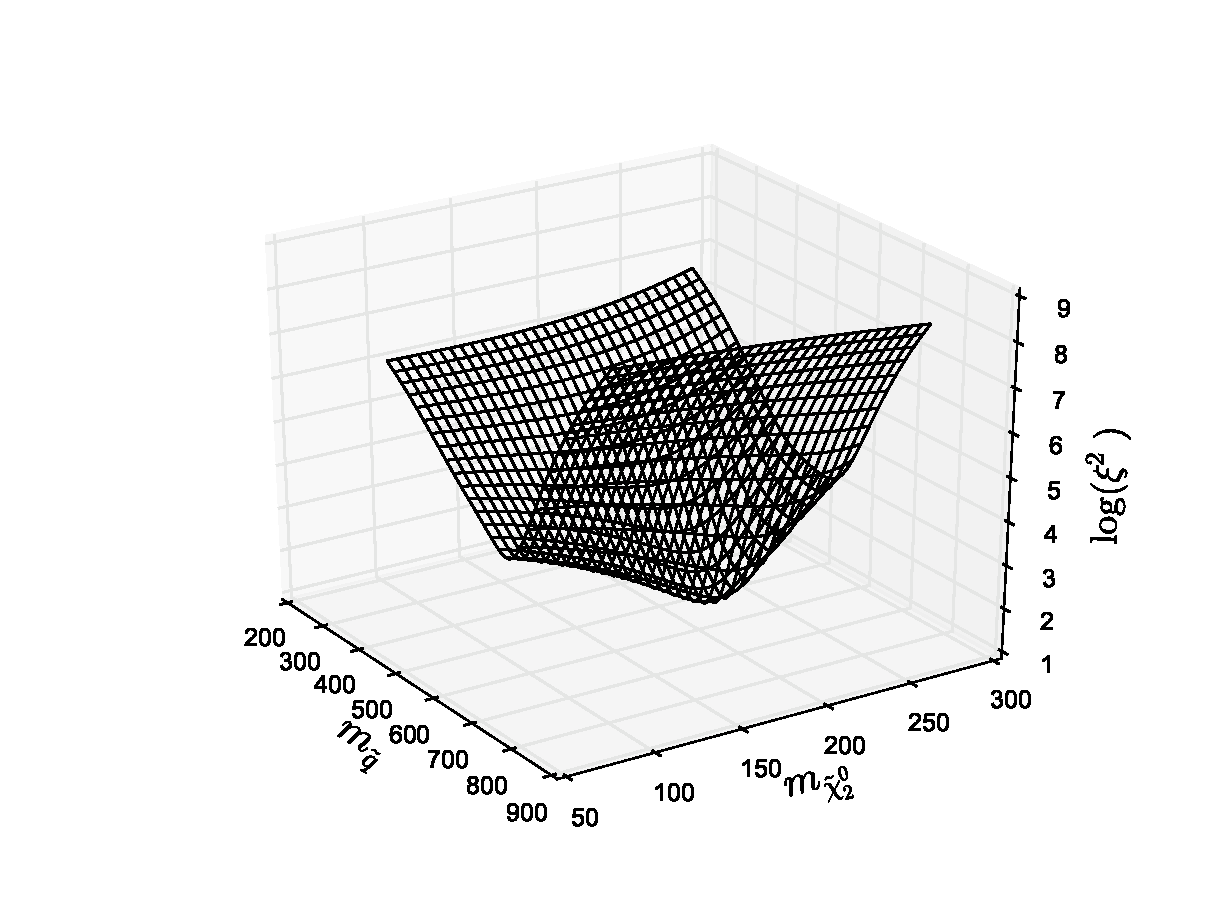
\includegraphics[width=\textwidth]{figures/3D_plot_xisquared_25_herwig_events_squark-chi2.pdf} 
		\caption{}
		\label{fig:3D_masses1}
	\end{subfigure}
	\begin{subfigure}[b]{0.49\textwidth}
		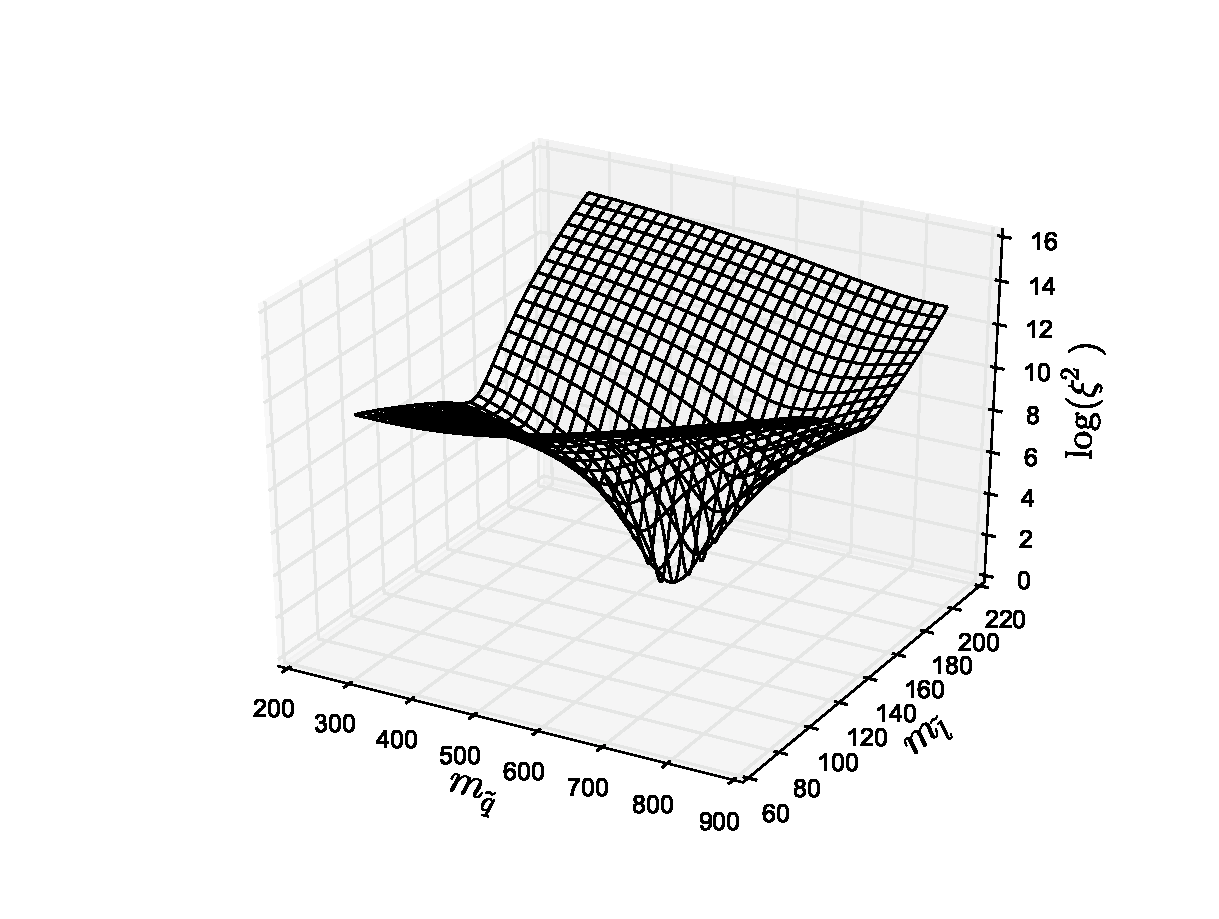
\includegraphics[width=\textwidth]{figures/3D_plot_xisquared_25_herwig_events_squark-slepton.pdf} 
		\caption{}
		\label{fig:3D_masses2}
	\end{subfigure}

	\begin{subfigure}[b]{0.49\textwidth}
		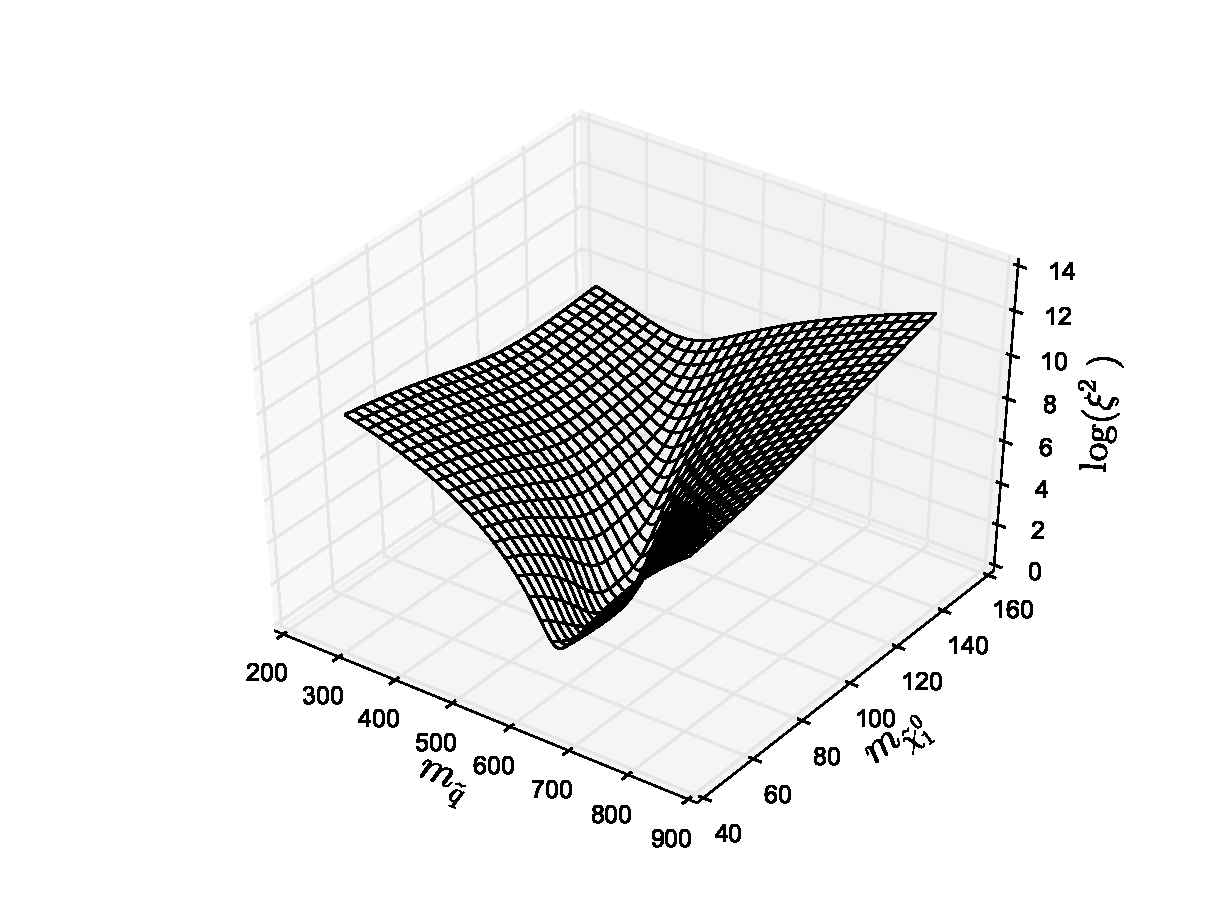
\includegraphics[width=\textwidth]{figures/3D_plot_xisquared_25_herwig_events_squark-chi1.pdf} 
		\caption{}
		\label{fig:3D_masses3}
	\end{subfigure}
	\begin{subfigure}[b]{0.49\textwidth}
		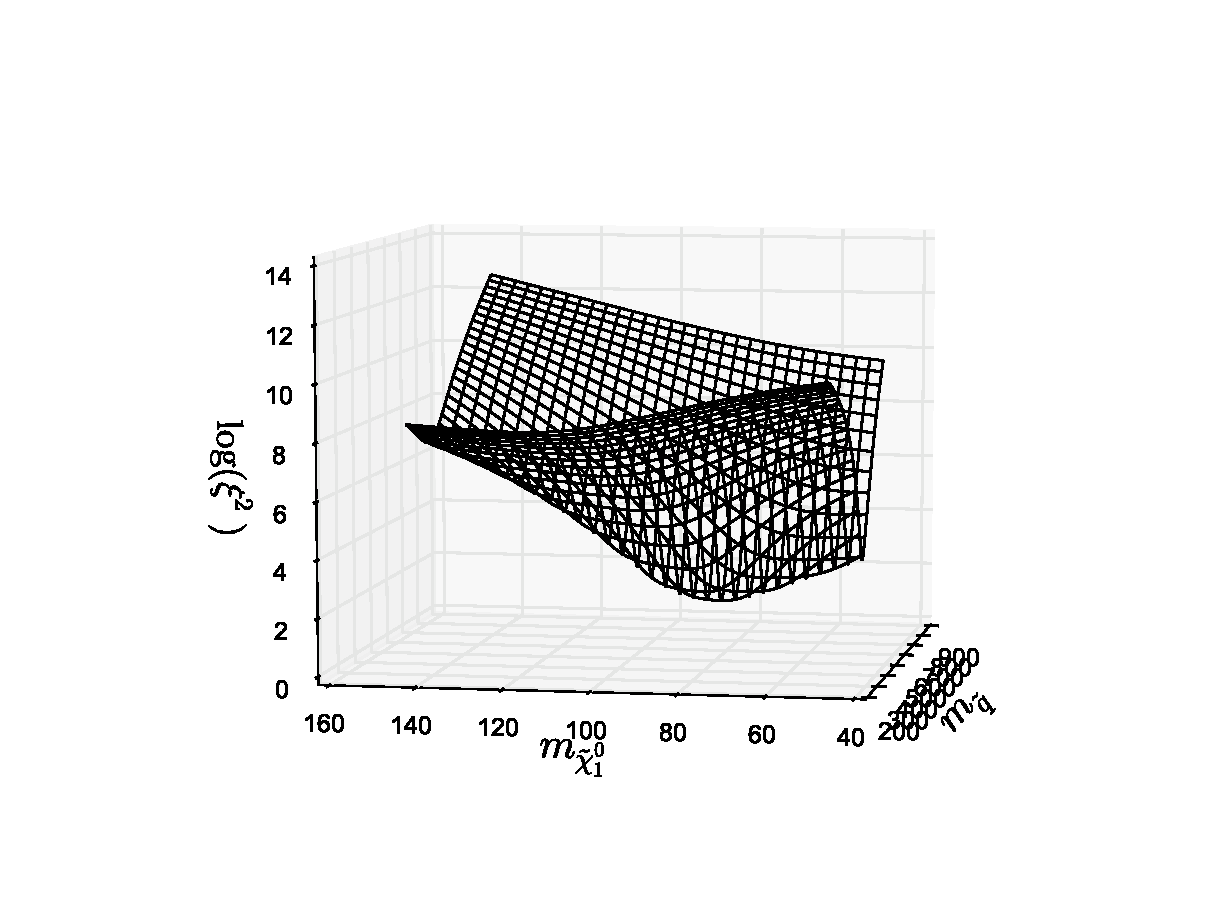
\includegraphics[width=\textwidth]{figures/3D_plot_xisquared_25_herwig_events_squark-chi1_rotated.pdf} 
		\caption{}
		\label{fig:3D_masses4}
	\end{subfigure}
	\caption{3D contour plot of $\log(\xi^2)$ in $m_{\tilde q}-m_i$ plane around the point of true minimum, where $i=\tilde \chi_2^0$ for (a), $i=\tilde l$ for (b) and $i=\tilde \chi_1^0$ for (c) and (d). The other two masses are fixed to their true value.}
	\label{fig:3D_masses}
\end{figure}\marginpar{Include $\xi^2$ surface plots. Discuss a bit more?} 
This is illustrated in fig.\ \ref{fig:3D_masses}, which shows contour plots of the $\xi^2$ for one event sample as function of pairs of mass parameters. We see that in this sample, the $\tilde \chi_1^0$ direction is flat at low mass values.

Setting the tolerance high may therefore lead to convergence at a non-minimal point. If, additionally, the search is started at or close to the masses used to generate the Monte Carlo, then the minimization may obtain ``convergence'' at points very close to the true value, but these points are not minimal points, just regions where the function is not very steep.

\section{The tolerance is too high}

Refer to the scatter plot in fig.\ 2 of \cite{Webber:2009vm}, displayed in fig.\ \ref{fig:webber_scatter} for convenience. This scatter plot shows the fit corresponding to the first row of table \ref{table:webber_original}. We have reproduced this fit using Webber's code \cite{Webber:epost} ---albeit with one modification: Since we do not have access to the {\tt ISAJET} and {\tt ISAWIG} software for RG running of SUSY parameters, we have generated our SPS 1a parameter point using {\tt SoftSUSY} version 3.4.1 \cite{Allanach:2001kg}, and converted the resulting SLHA \cite{Skands:2003cj} model file to {\tt ISAWIG} format using the package {\tt PySLHA} version 3.0.2\footnote{We have had to make several modifications to the {\tt PySLHA} code to make the {\tt ISAWIG} output readable by {\tt HERWIG}. These changes have been included in {\tt PySLHA} 3.0.3.} \cite{Buckley:2013jua}. The effects of using a different RG runner is that the SUSY masses are not exactly the same. The most significant shift is the squarks, which in Webber's case have a mass of 540 GeV, compared to 565 GeV in our case. We observe similar results as Webber gives in his article when we run his code with the original settings for our SUSY parameter point. 
\begin{figure}[hbt]
	\centering
	\begin{subfigure}[b]{0.8\textwidth}
		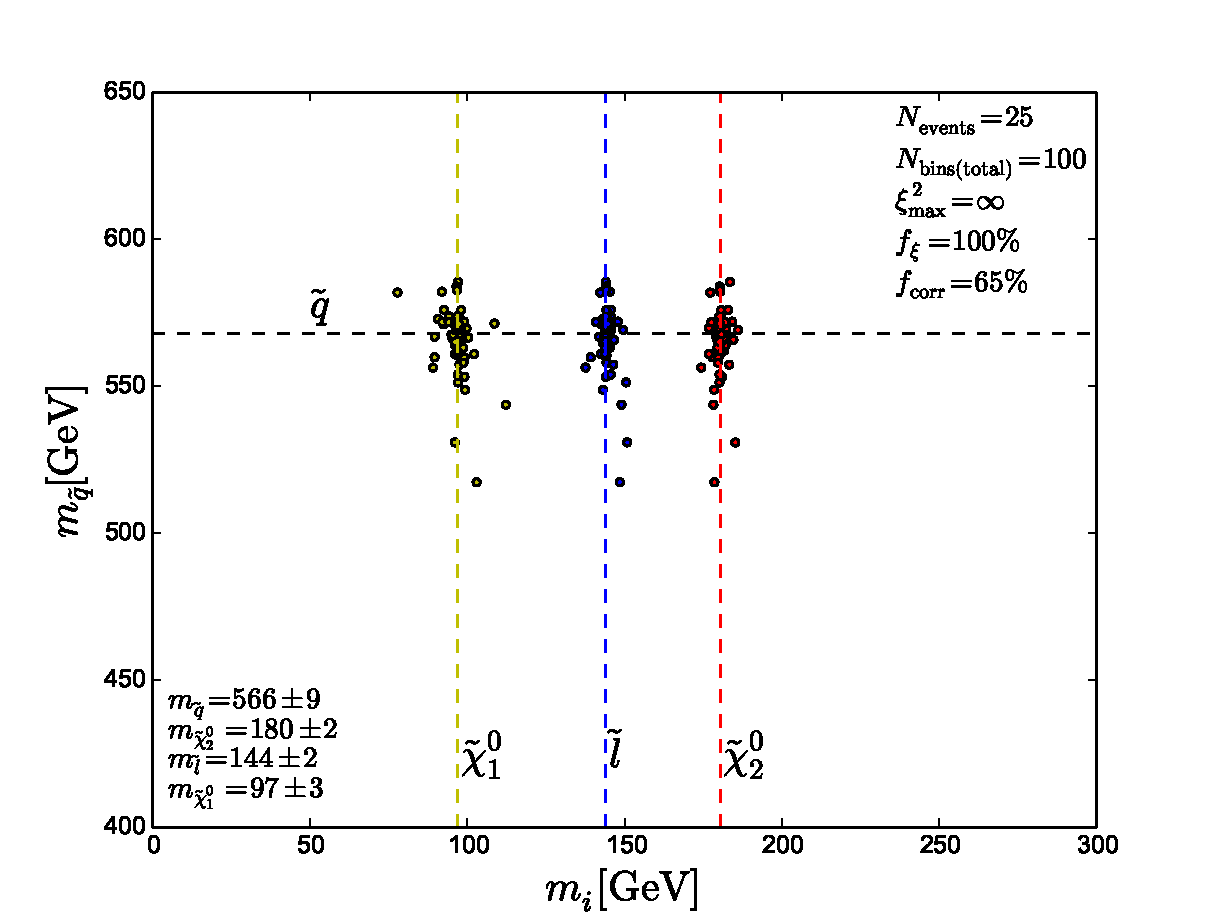
\includegraphics[width=\textwidth]{figures/webber_rec_table/webber_rec_table-samesettings_0psmear-nocut.pdf} 
		\caption{ }
		\label{fig:webber_rec_scatter_tolerance-comparison_a}
	\end{subfigure}

	\begin{subfigure}[b]{0.8\textwidth}
		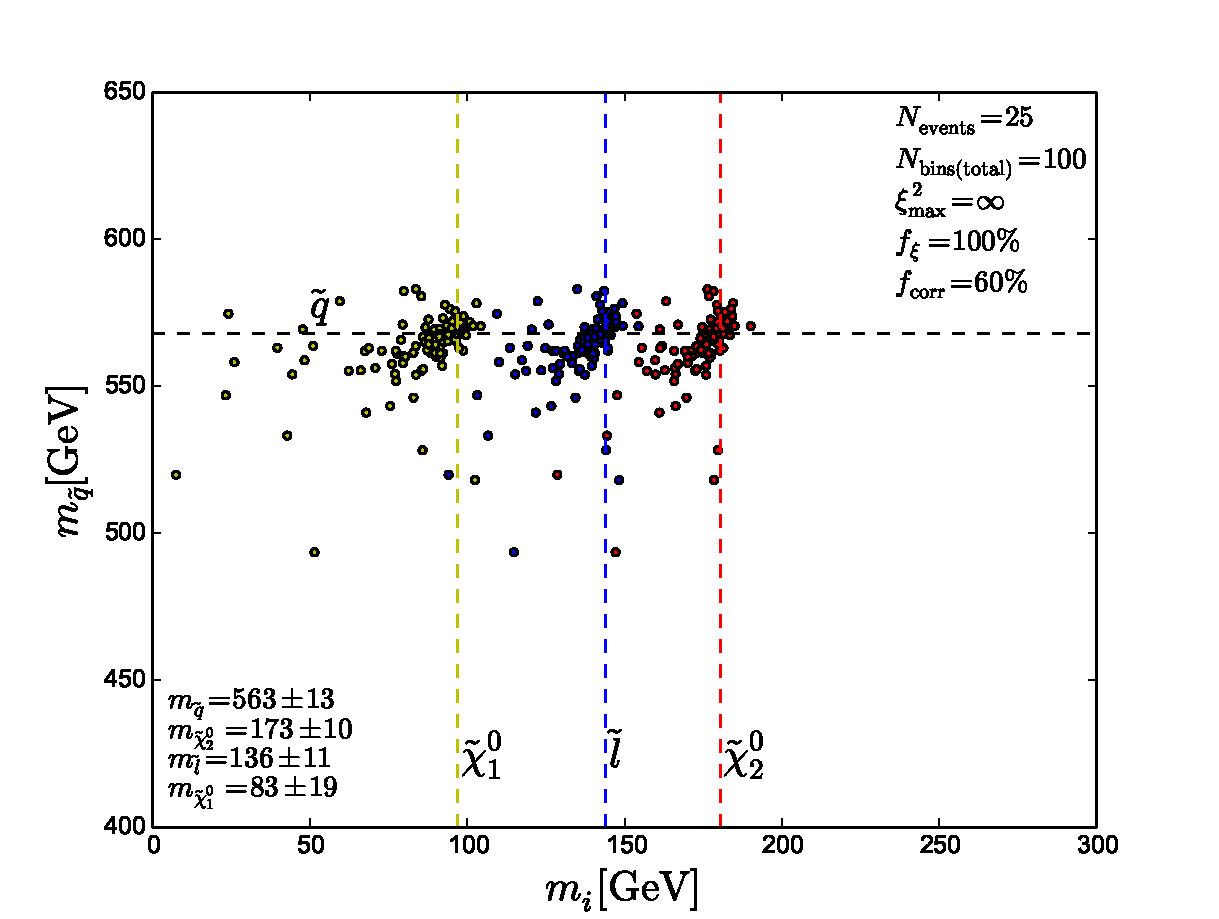
\includegraphics[width=\textwidth]{figures/webber_rec_table/webber_HW-rec_nocut.pdf}
		\caption{ } 
		\label{fig:webber_rec_scatter_tolerance-comparison_b}
	\end{subfigure}
	\caption{Reproduction of Webber's results (corresponding to fig. \ref{fig:webber_scatter} and the first row of table \ref{table:webber_original}) for (a) original convergence tolerance and (b) a lower tolerance criterion.}
	\label{fig:webber_rec_scatter_tolerance-comparison}
\end{figure}
Our reproduction of fig.\ \ref{fig:webber_scatter} is shown in fig.\ \ref{fig:webber_rec_scatter_tolerance-comparison_a}\footnote{All the scatter plots in this thesis are in vector graphics format. When the thesis is viewed electronically, they are zoomable.}, and our reproduction of table \ref{table:webber_original} is given in table \ref{table:webber_softsusy}.
\begin{table}[hbt]
	\centering
	\begin{tabular}{| l | l | l | l  || l | l | l | l |}
		\hline
		$\delta p/p$ & $\xi^2_\mathrm{max}$ & $f_\xi$ & $f_\mathrm{corr}$ & $m_{\tilde q} (540)$ & $m_{\tilde \chi_2^0} (177)$ & $m_{\tilde l} (143)$ & $m_{\tilde \chi_1^0} (96)$ \\
		\hline \hline
		0 & 	$\infty$ &	100 \%	& 65 \%	& $566 \pm 9$	&	$180 \pm 2$		&	$144 \pm 2$	& 	$97 \pm 3$	\\
		0 &		100 &		85 \%	& 67 \% & $567 \pm 6$	&	$180 \pm 1$		&	$144 \pm 1$	&	$97 \pm 3$	\\
		5 \% &	$\infty$ &	100 \%	& 43 \% & $564 \pm 26$	& 	$181 \pm 14$	&	$145 \pm 10$&	$94 \pm 15$ \\
		5 \% &	100 &		52 \%	& 48 \% & $566 \pm 10$	&	$180 \pm 2$		& 	$145 \pm 2$	&	$96 \pm 4$	\\
		10 \% &	$\infty$ &	100 \%	& 33 \% & $551 \pm 33$	&	$180 \pm 15$	&	$144 \pm 11$&	$91 \pm 24$	\\
			10 \% &	200 &		43 \%	& 36 \% & $559 \pm 17$	& 	$177 \pm 11$	&	$143 \pm 11$&	$91 \pm 20$ \\
		\hline
	\end{tabular}
	\caption{Our reproduction of table \ref{table:webber_original}, using Webber's code \cite{Webber:epost} with original settings, except with the masses from SoftSUSY.}
	\label{table:webber_softsusy}
\end{table}

However, the tolerance setting in {Minuit} can be adjusted. When we rerun the code used to produce fig.\ \ref{fig:webber_rec_scatter_tolerance-comparison_a} with the tolerance set to $10^{-12}$, we get the fit shown in \ref{fig:webber_rec_scatter_tolerance-comparison_b}. The results are not dramatically altered, but there are some features to notice: There is a clear tendency to a linear correlation between the masses. This is a feature we should expect physically: If one reduces one of the masses, {\it e.g.}\ the squark, then this should affect the fit of the other masses, reducing them correspondingly.\footnote{This is part of the reason why these kinds of mass reconstruction methods very often reconstruct the squared mass {\it difference} rather than the masses themselves.} The fact that this physically reasonable degenerate direction appears when the tolerance is reduced indicates that a such a reduction is necessary to achieve reliable results. We also note that the fitted masses now seem slightly biased toward lower values. Finally we note that while the mean value and errors are still consistent with the true values, their accuracy is somewhat reduced. Particularly so for the LSP, where the fit is reduced from $99 \pm 3$ GeV to $83 \pm 19$ GeV, compared to the true value of 97 GeV.

These fit results, with the low tolerance setting, are still not bad. However, in table \ref{table:webber_original}, Webber also gives best-fit values where he has applied smearing to the four-momenta, as a crude approximation to the effects of limited detector resolution. The momentum smearing is done by smearing the spatial components according to a gaussian distribution of a given r.m.s. width $\delta p/p$, and then defining the energy in such a way that the invariant mass is unchanged \cite{Webber:epost}.
\begin{figure}[hbtp!]
	\centering
	\begin{subfigure}[b]{0.8\textwidth}
		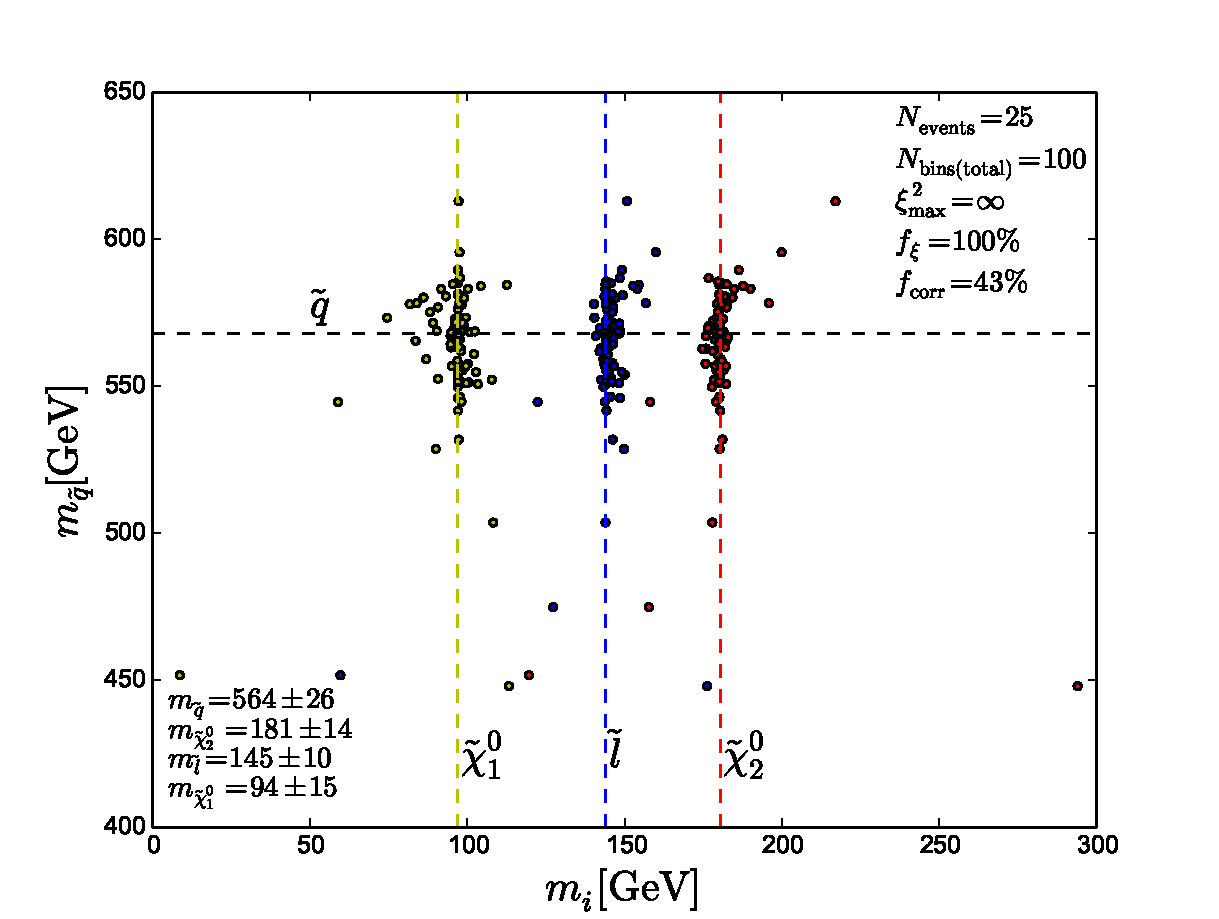
\includegraphics[width=\textwidth]{figures/webber_rec_table/webber_HW-rec_OFL_minuit-minimizer_hightol_5pmomsmear_nocut.pdf} 
		\caption{ }
	\end{subfigure}

	\begin{subfigure}[b]{0.8\textwidth}
		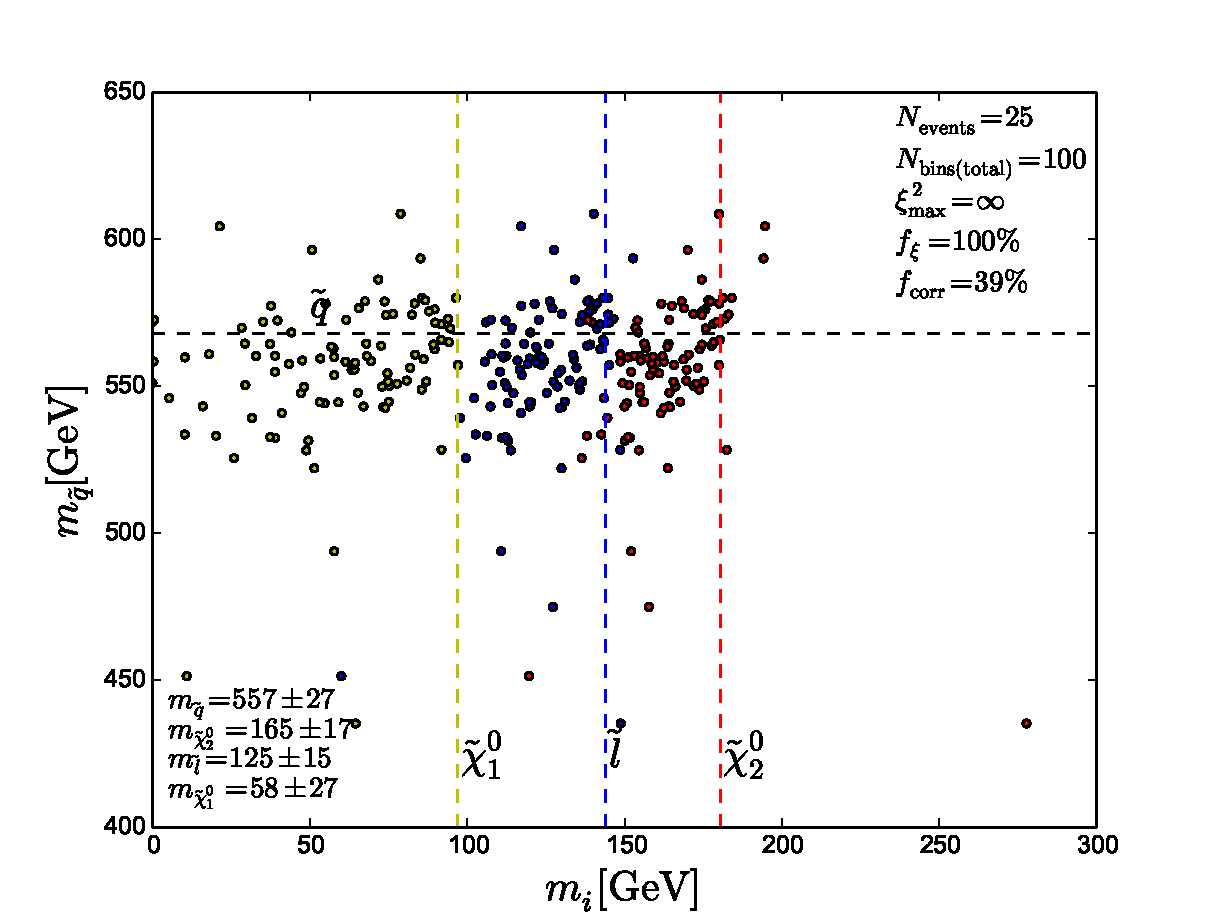
\includegraphics[width=\textwidth]{figures/webber_rec_table/webber_HW-rec_OFL_minuit-minimizer_lowtol_5pmomsmear_nocut.pdf}
		\caption{ } 
	\end{subfigure}
	\caption{Reproduction of Webber's 5\% momentum-smeared fit (corresponding to the third row of table \ref{table:webber_original}) for (a) original convergence tolerance and (b) a lower tolerance criterion.}
	\label{fig:webber_rec_scatter_tolerance-comparison_5pmomsmear}
\end{figure} 
In fig.\ \ref{fig:webber_rec_scatter_tolerance-comparison_5pmomsmear} we show scatter plots of the fits to the dataset smeared with $\delta p/p = 5 \%$, minimized with original and reduced tolerance, again using Webber's code for event generation and minimization. The fit with original tolerance is consistent with fig.\ 3 of \cite{Webber:2009vm}, as it should be. However, when the tolerance is reduced, the fit results are worsened considerably. Since each event is smeared individually, this appears to greatly affect the position of the minimum. Again we see that the LSP (yellow) recieves the roughest treatment, being pushed to much lower values than the true one in most cases. The results are even worse for the 10 \% smeared dataset. 
%We also note that in the {\tt HERWIG} code Webber uses, initial-state radiation of photons in SUSY decays is switched off, which may contribute to making the measurement unrealistically good.\marginpar{Are doesn't think this is a big effect, but I am not sure. I did complete momentum conservation in my events same as Webber, in practice turning off ISR. Should consider checking, or rewriting.}




% \begin{figure}[hbt]
% 	\centering
% 	\begin{subfigure}[b]{0.6\textwidth}
% 		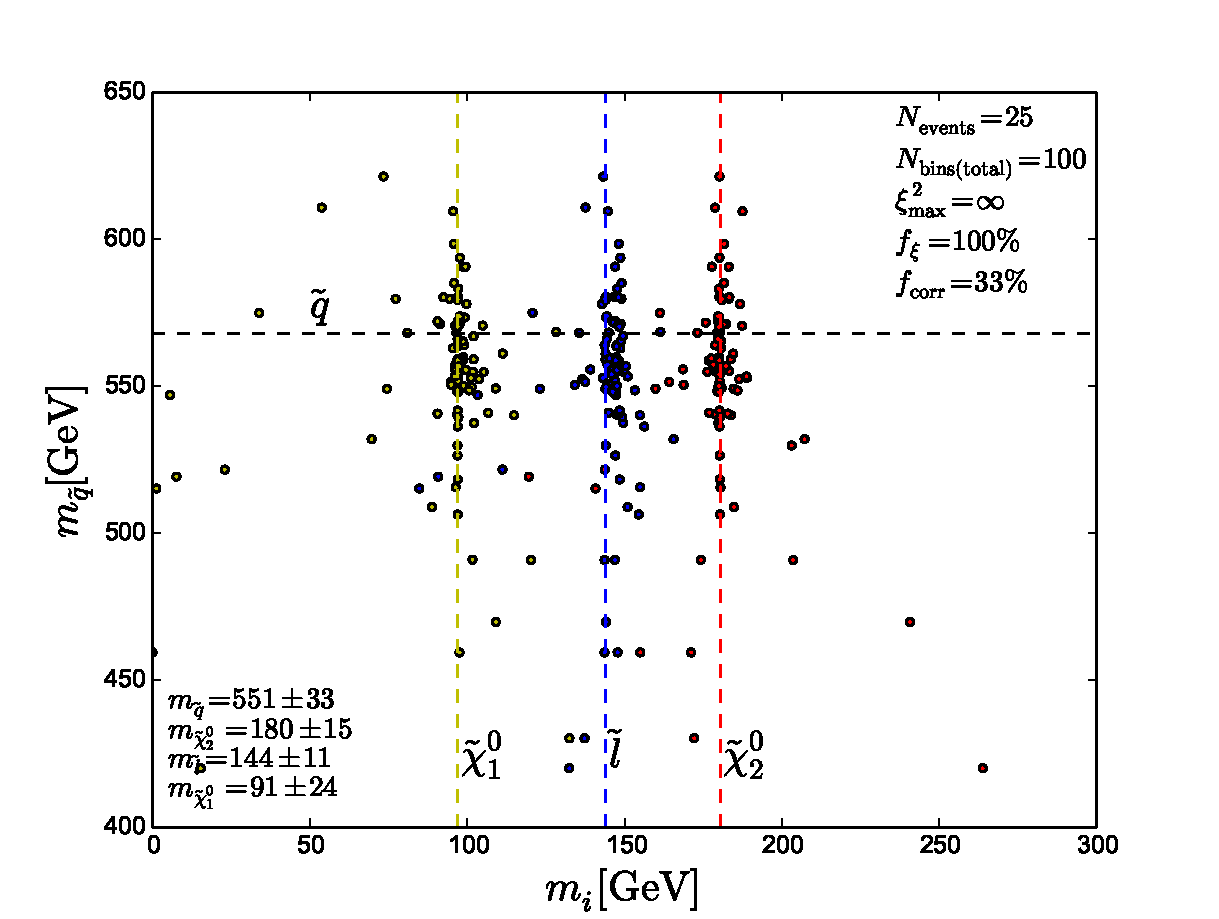
\includegraphics[width=\textwidth]{figures/webber_rec_table/webber_HW-rec_OFL_minuit-minimizer_hightol_10pmomsmear_nocut.pdf} 
% 		\caption{ }
% 	\end{subfigure}

% 	\begin{subfigure}[b]{0.6\textwidth}
% 		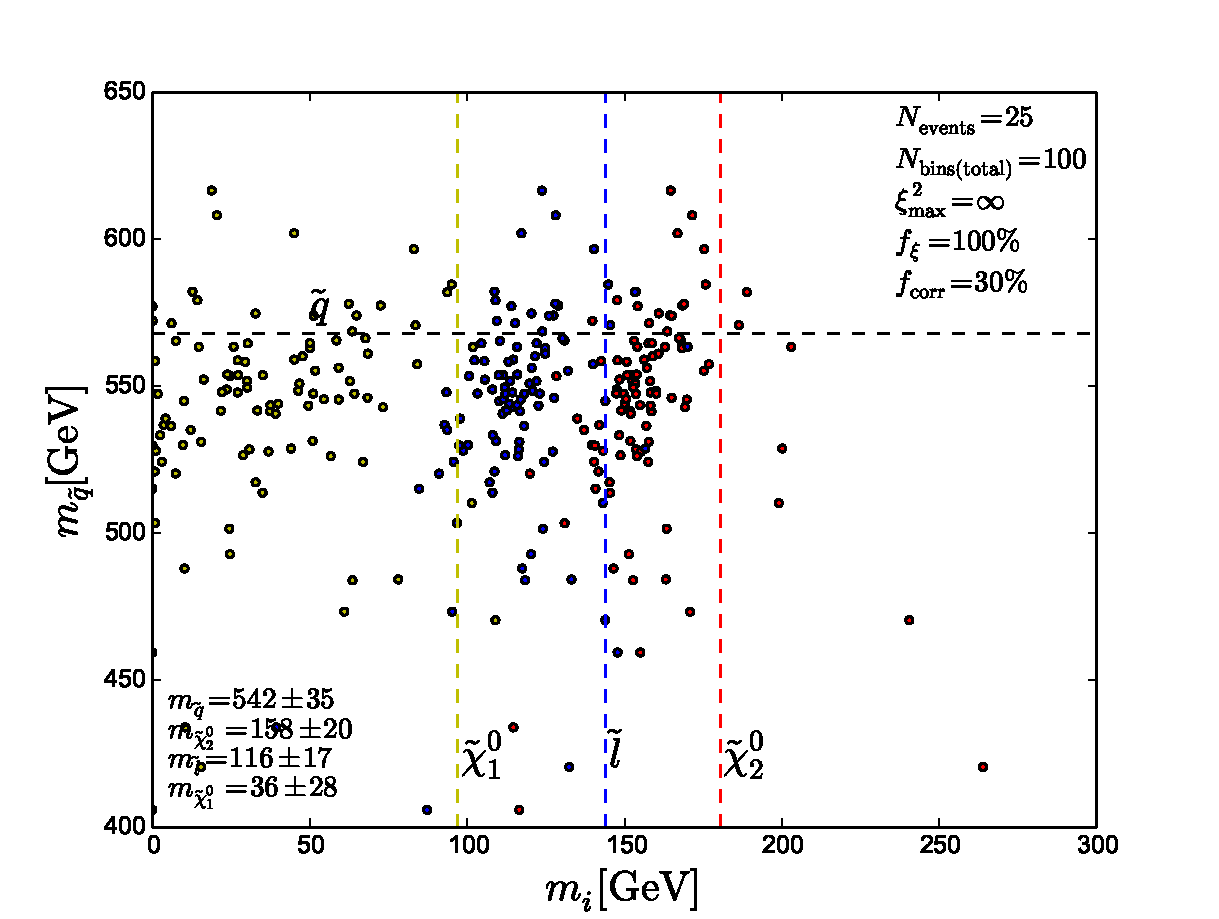
\includegraphics[width=\textwidth]{figures/webber_rec_table/webber_HW-rec_OFL_minuit-minimizer_lowtol_10pmomsmear_nocut.pdf}
% 		\caption{ } 
% 	\end{subfigure}
% 	\caption{Reproduction of Webber's 10 \% momentum-smeared fit (corresponding to fig. 3 of \cite{Webber:2009vm} and the fifth row of table \ref{table:webber_original}) for (a) original convergence tolerance and (b) a lower tolerance criterion.}
% 	\label{fig:webber_rec_scatter_tolerance-comparison_10pmomsmear}
% \end{figure}

However, Webber also investigates the effects of imposing a {\it cut} on the $\xi^2$ value obtained at the minimum. In his fits, this cut tends to remove the bad events, giving a better fit. Applying a cut also helps for the reduced-tolerance fit, although it does not recover Webber's original low error estimate. In table \ref{table:webber_rec_lowtol} we reproduce table \ref{table:webber_original} for the reduced-tolerance fit. We note that the fraction of samples passing the $\xi^2$ cut is drastically reduced compared to table \ref{table:webber_original}. The fraction of events where the best-fit combination is the true one is also reduced by about half. 

\begin{table}[hbt]
	\centering
	\begin{tabular}{| l | l | l | l  || l | l | l | l |}
		\hline
		$\delta p/p$ & $\xi^2_\mathrm{max}$ & $f_\xi$ & $f_\mathrm{corr}$ & $m_{\tilde q} (568)$ & $m_{\tilde \chi_2^0} (180)$ & $m_{\tilde l} (144)$ & $m_{\tilde \chi_1^0} (97)$ \\
		\hline \hline
		0 & 	$\infty$ &	100 \%	& 36 \%	& $563 \pm 13$	&	$173 \pm 10$	&	$136 \pm 11$	& 	$83 \pm 19$	\\
		0 &		100 &		35 \%	& 52 \% & $565 \pm 9$	&	$175 \pm 8$		&	$138 \pm 9$	&	$86 \pm 16$	\\
		5 \% &	$\infty$ &	100 \%	& 31 \% & $557 \pm 27$	& 	$165 \pm 17$	&	$125 \pm 15$&	$58 \pm 27$ \\
		5 \% &	100 &		13 \%	& 43 \% & $558 \pm 14$	&	$164 \pm 11$	& 	$126 \pm 12$	&	$65 \pm 22$	\\
		10 \% &	$\infty$ &	100 \%	& 29 \% & $542 \pm 35$	&	$158 \pm 20$	&	$116 \pm 17$&	$36 \pm 28$	\\
		10 \% &	200 &		15 \%	& 33 \% & $549 \pm 20$	& 	$155 \pm 12$	&	$116 \pm 12$&	$38 \pm 25$ \\
		\hline
	\end{tabular}
	\caption{Reproduction of the fits in table \ref{table:webber_softsusy}, but with reduced convergence tolerance.}
	\label{table:webber_rec_lowtol}
\end{table}

\section{The starting-point dependence of the best-fit point}
\label{sec:SP-dependence_webber}
There is also another potential issue with Webber's analysis. It has to do with the fact that the best-fit search is started at the true mass values.  In a real experiment, these parameters are the unknowns we wish to find. Starting the search here is in principle fine as long as we are sure that the algorithm always finds the true global minimum. So we must investigate what happens if we start our search in some other point. We have done this, and discover that this greatly affects the location of the best-fit points.
\begin{figure}[hbt]
	\centering
	\begin{subfigure}[b]{0.45\textwidth}
		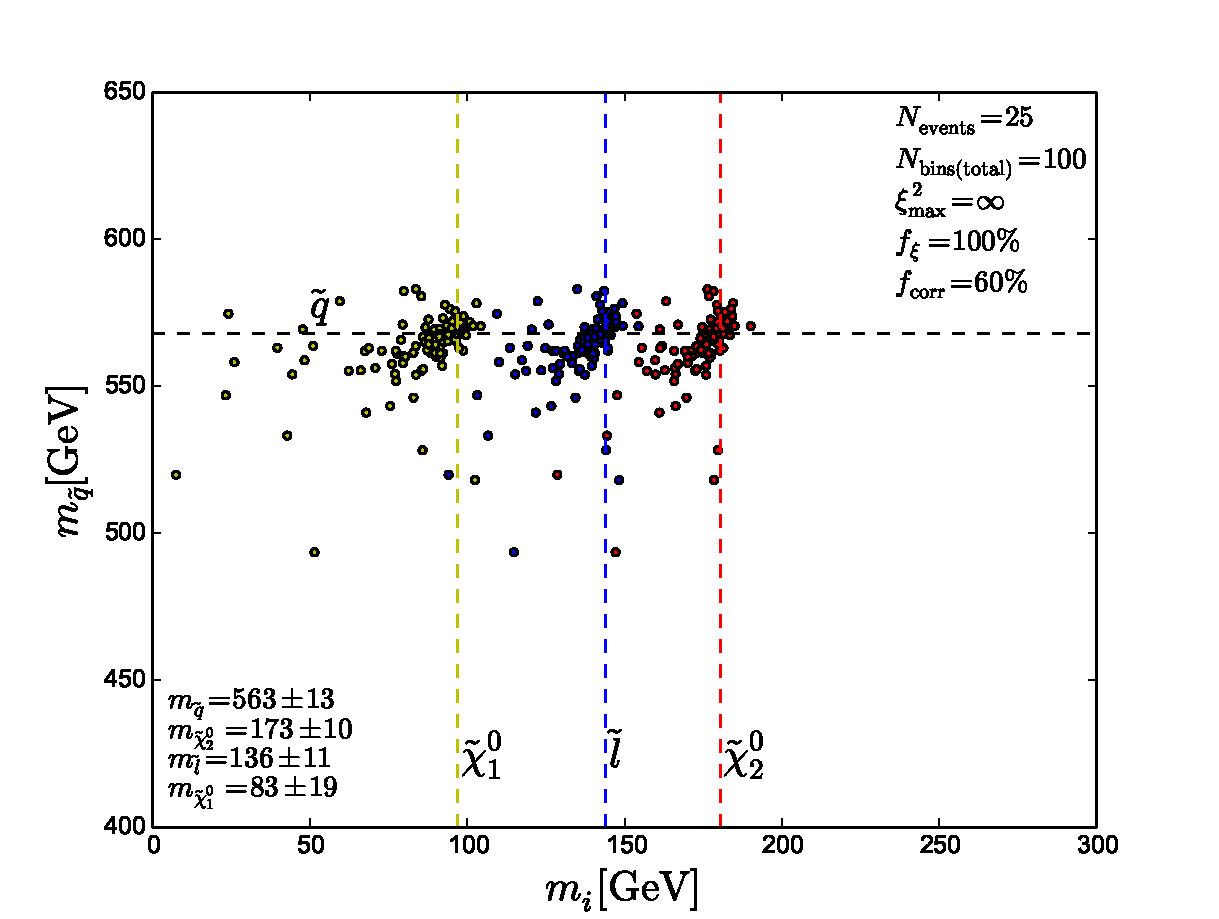
\includegraphics[width=\textwidth]{figures/webber_rec_table/webber_HW-rec_nocut.pdf} 
		\caption{ }
	\end{subfigure}
	\begin{subfigure}[b]{0.45\textwidth}
		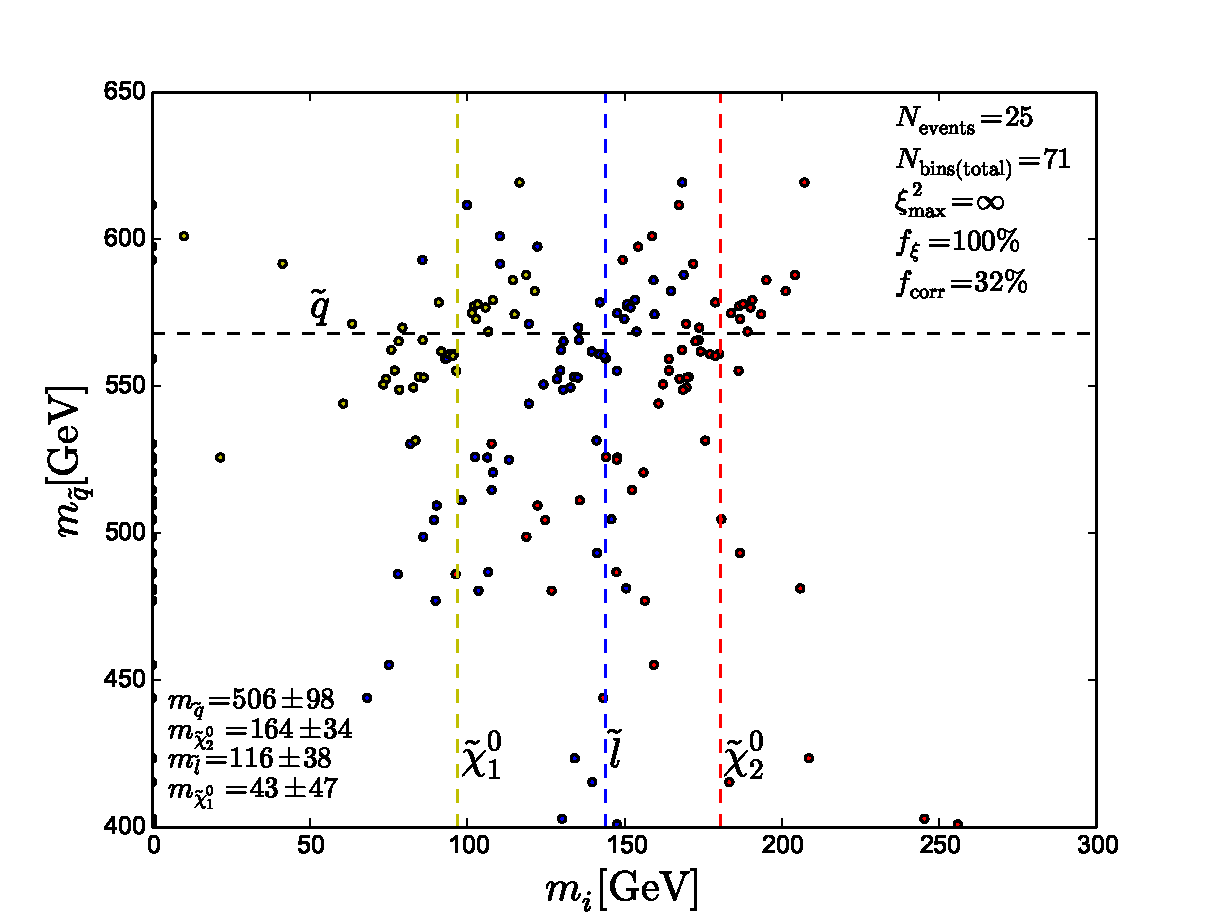
\includegraphics[width=\textwidth]{figures/webber_rec_table/webber-rec_wrong_starting_point-400-300-200-100_lowtol.pdf}
		\caption{ } 
	\end{subfigure}

	\begin{subfigure}[b]{0.45\textwidth}
		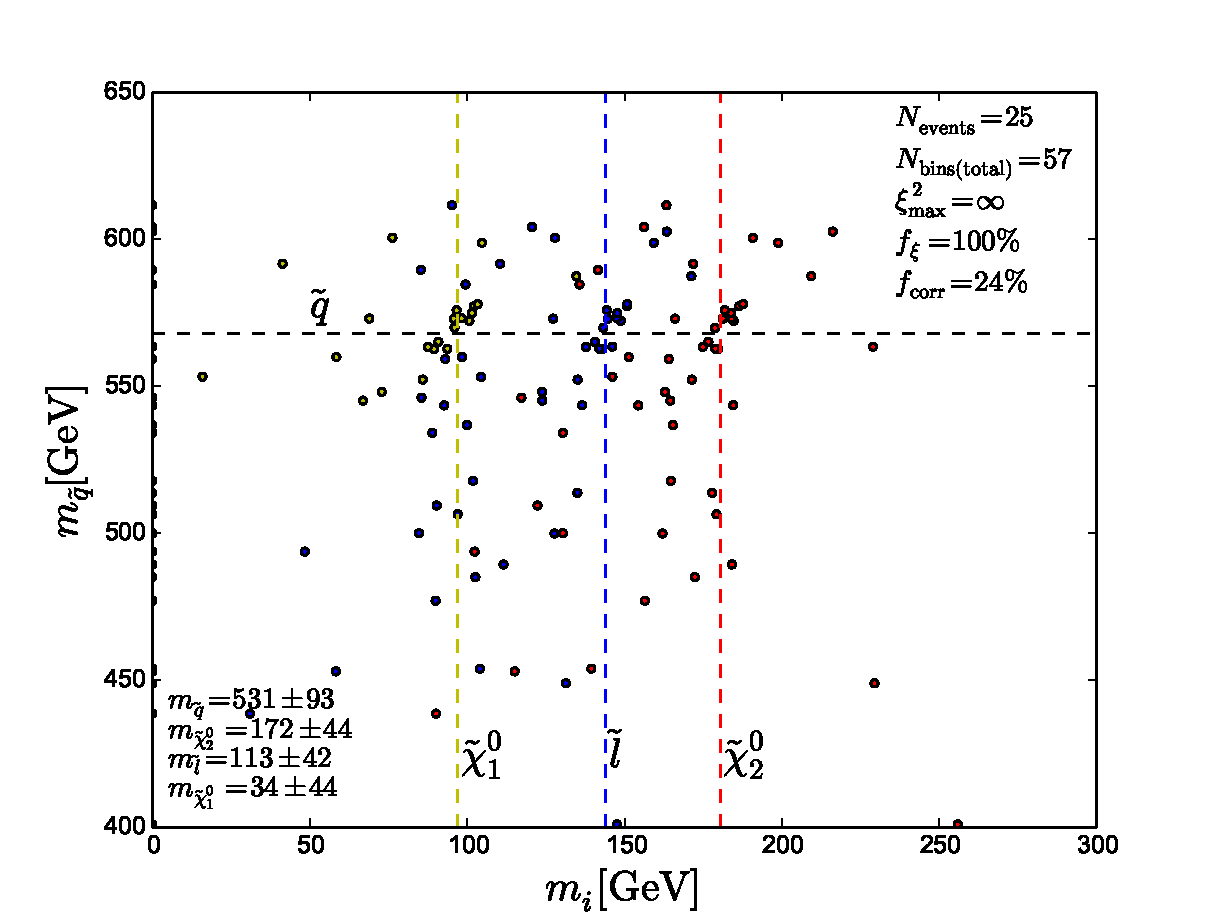
\includegraphics[width=\textwidth]{figures/webber_rec_table/webber-rec_wrong_starting_point-800-500-300-50_lowtol.pdf} 
		\caption{ }
	\end{subfigure}
	\begin{subfigure}[b]{0.45\textwidth}
		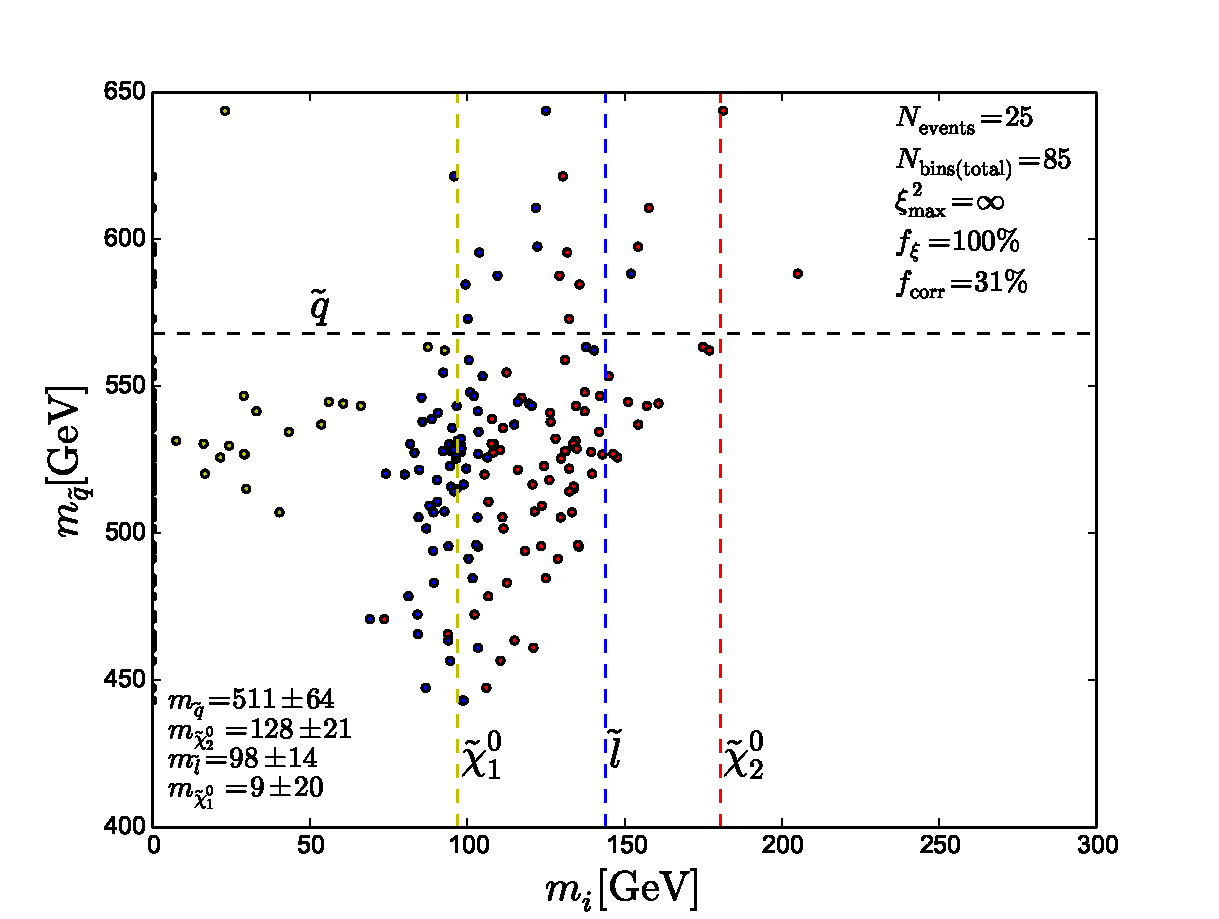
\includegraphics[width=\textwidth]{figures/webber_rec_table/webber-rec_wrong_starting_point-1000-100-80-30_lowtol.pdf}
		\caption{ } 
	\end{subfigure}
	\caption{Minimization on the unsmeared {\tt HERWIG} dataset for different starting points: $\vec M = (568, 180, 144, 97)$ (the TMP) in {\bf (a)}, $\vec M = (400, 300, 200, 100)$  in {\bf (b)}, $\vec M = (800, 500, 300, 50)$ in {\bf (c)} and $\vec M = (1000, 100, 80, 30)$ in {\bf (d)}.}
	\label{fig:starting_point_sensitivity_combinatorics}
\end{figure}
In fig.\ \ref{fig:starting_point_sensitivity_combinatorics} we show the best-fit points for four low-tolerance minimizations on the {\tt HERWIG} dataset. Subfig.\ (a) is the same as \ref{fig:webber_rec_scatter_tolerance-comparison} (b), the minimization started from the true mass point (TMP). The other three are minimizations from other starting points, selected to illustrate other plausible mass spectra: one where both the masses and the mass differences are smaller (b); one where they are larger (c); and one where there is a large splitting between a heavy squark and three very light masses (d). It is obvious that the fit ---the location of the best-fit point, and also the number of samples where convergence is obtained, indicated by the number $N_\mathrm{bins}$ in each plot ---is hugely dependent on where we start the search. For instance, the mean value and standard errors of the squark masses for the samples range from $506 \pm 98~\mathrm{GeV}$ to $563 \pm 13~\mathrm{GeV}$. We also note that the margins of error in the latter case, which is minimization from the TMP, exclude the mean values obtained from the other three starting points.



It might, however, be that the function has multiple local minima, giving rise to the behaviour in fig.\ \ref{fig:starting_point_sensitivity_combinatorics}, but that the {\it global} minimum is the one we find by starting in the TMP. To investigate this, we have run minimizations (with low tolerance) where we perturb the starting point of each of the four parameters for each event sample away from the TMP by a gaussian distribution of width 10 or 20 GeV. This is a minor perturbation relative to the masses. The minimization results are shown in table \ref{table:webber_rec_lowtol_perturbedSP} for perturbations of 10 (top) and 20 (bottom) GeV. The standard errors of the fit increase considerably compared with \ref{table:webber_rec_lowtol}. \marginpar{Smear with 10 \% and 20 \% of the masses too?}
 
% we have made a scan of many starting points, minimizing the whole 100 bin dataset from each starting point. We selected five different values for each of the four SUSY masses and checked all combinations which make physical sense ({\it i.e.\ }where the mass hierarchy is present). This gave a total of 132 different starting points, which were indexed from 1 to 132. The TMP was point number 34. For each bin we then checked which index had the lowest $\xi^2$ value. Figure \ref{fig:webber_rec_hist_starting_points} shows a histogram of this. We see that number 34, the TMP, indeed dominates, but it is only the lowest in 14 of the 100 bins. The other 86 bins are distributed quite evenly among the other starting points. This leads us to conclude that the minimization, using this technique, simply is not well defined: There is no reasonable hope that we will be able to find a reliable best-fit estimate in an experimental situation where the TMP is unknown. This is especially true given that this scan was done on the unsmeared dataset ---we should expect even worse results when the resolution gets blurred by uncertainties.

% \begin{figure}[hbt]
% 	\centering
% 	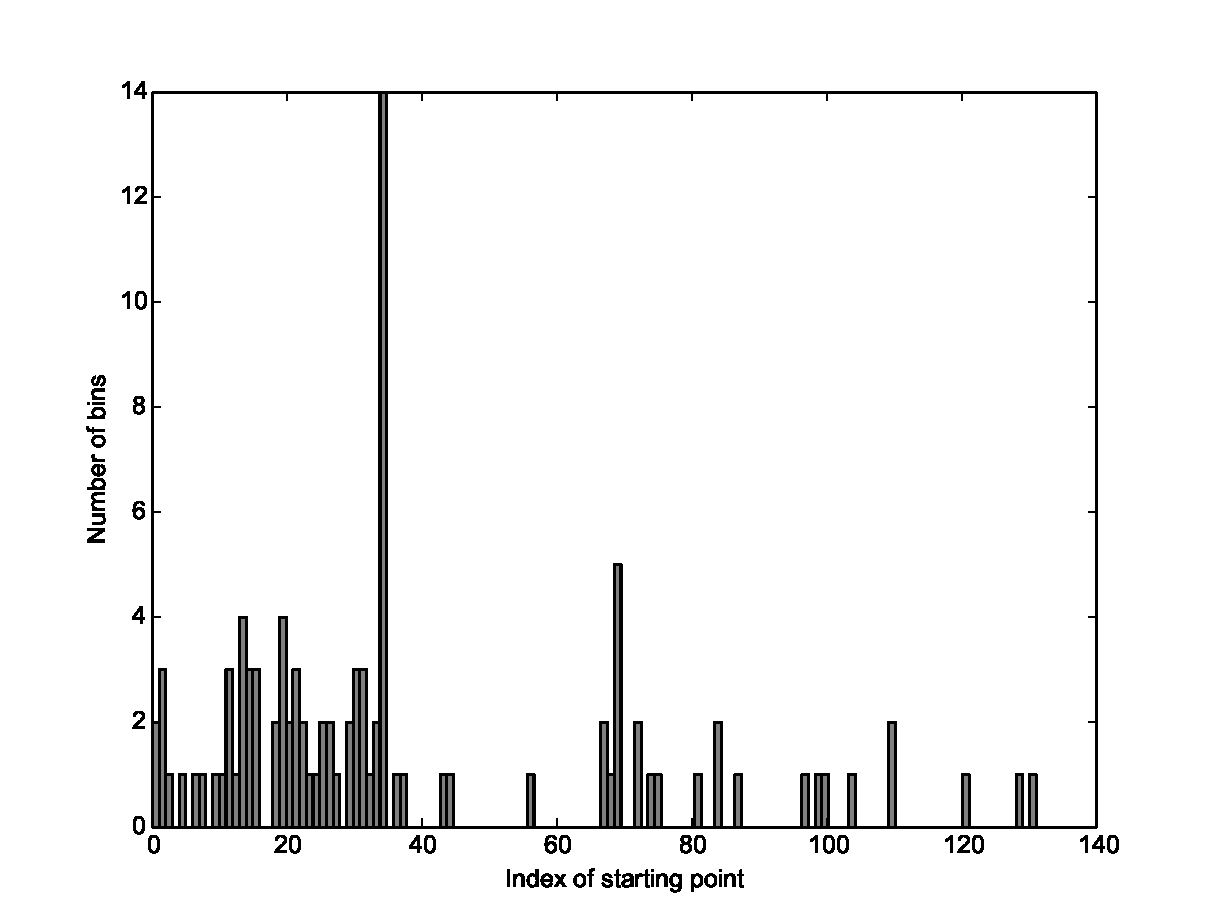
\includegraphics[width=0.8\textwidth]{figures/webber_rec_table/histogram_of_starting_points_with_lowest_minimal_value.pdf}
% 	\caption{A histogram of 100 data bins minimized from different starting points, showing distribution of lowest $\xi^2$ values. See the text for details.}
% 	\label{fig:webber_rec_hist_starting_points}
% \end{figure}


\begin{table}[hbt]
	\centering
	\begin{tabular}{| l | l | l | l  || l | l | l | l |}
		\hline
		$\delta p/p$ & $\xi^2_\mathrm{max}$ & $f_\xi$ & $f_\mathrm{corr}$ & $m_{\tilde q} (568)$ & $m_{\tilde \chi_2^0} (180)$ & $m_{\tilde l} (144)$ & $m_{\tilde \chi_1^0} (97)$ \\
		\hline \hline
		10 GeV: & & & & & & & \\ 
		\hline
		0 & 	$\infty$ &	100 \%	& 47 \%	& $559 \pm 29$	&	$170 \pm 19$	&	$131 \pm 20$	& 	$68 \pm 38$	\\
		0 &		100 &		76 \%	& 48 \% & $564 \pm 12$	&	$175 \pm 13$		&	$137 \pm 14$	&	$83 \pm 25$	\\
		5 \% &	$\infty$ &	100 \%	& 38 \% & $557 \pm 24$	& 	$163 \pm 18$	&	$123 \pm 20$&	$52 \pm 36$ \\
		5 \% &	100 &		55 \%	& 37 \% & $559 \pm 16$	&	$168 \pm 13$	& 	$130 \pm 15$	&	$72 \pm 22$	\\
		10 \% &	$\infty$ &	100 \%	& 28 \% & $542 \pm 42$	&	$153 \pm 19$	&	$113 \pm 21$&	$19 \pm 31$	\\
		10 \% &	200 &		44 \%	& 26 \% & $550 \pm 21$	& 	$159 \pm 18$	&	$119 \pm 20$&	$38 \pm 36$ \\
		\hline
		20 GeV: & & & & & & & \\ 
		\hline
		0 & 	$\infty$ &	100 \%	& 42 \%	& $555 \pm 32$	&	$167 \pm 23$	&	$126 \pm 24$	& 	$60 \pm 41$	\\
		0 &		100 &		67 \%	& 44 \% & $564 \pm 14$	&	$173 \pm 14$	&	$135 \pm 16$	&	$82 \pm 24$	\\
		5 \% &	$\infty$ &	100 \%	& 34 \% & $550 \pm 45$	& 	$162 \pm 23$	&	$123 \pm 22$&	$46 \pm 39$ \\
		5 \% &	100 &		54 \%	& 34 \% & $554 \pm 23$	&	$163 \pm 21$	& 	$125 \pm 21$	&	$63 \pm 31$	\\
		10 \% &	$\infty$ &	100 \%	& 28 \% & $543 \pm 37$	&	$153 \pm 25$	&	$125 \pm 21$&	$16 \pm 32$	\\
		10 \% &	200 &		37 \%	& 27 \% & $539 \pm 22$	& 	$151 \pm 20$	&	$113 \pm 18$&	$24 \pm 31$ \\
		\hline
	\end{tabular}
	\caption{Reproduction of the fits in table \ref{table:webber_rec_lowtol} with perturbations of 10 and 20 GeV, respectively, on the starting points.}
	\label{table:webber_rec_lowtol_perturbedSP}
\end{table}



\clearpage

\section{Without combinatorics}

If we for a moment forget about the combinatorics, and evaluate only the true particle combination for each event, then the minimization gives consistent results irrespective of starting point. 
\begin{figure}[hbt]
	\centering
	\begin{subfigure}[b]{0.45\textwidth}
		\includegraphics[width=\textwidth]{figures/improving_combinatorics/herwigpp-momcons_nocomb_truemasspoint.pdf} 
		\caption{ }
	\end{subfigure}
	\begin{subfigure}[b]{0.45\textwidth}
		\includegraphics[width=\textwidth]{figures/improving_combinatorics/herwigpp-momcons_nocomb_400-300-200-100.pdf}
		\caption{ } 
	\end{subfigure}

	\begin{subfigure}[b]{0.45\textwidth}
		\includegraphics[width=\textwidth]{figures/improving_combinatorics/herwigpp-momcons_nocomb_800-500-300-50.pdf} 
		\caption{ }
	\end{subfigure}
	\begin{subfigure}[b]{0.45\textwidth}
		\includegraphics[width=\textwidth]{figures/improving_combinatorics/herwigpp-momcons_nocomb_1000-100-80-30.pdf}
		\caption{ } 
	\end{subfigure}
	\caption{An equivalent fit to fig. \ref{fig:starting_point_sensitivity_combinatorics} (on a {\ttfamily Herwig++} dataset), but the $\xi^2$ contribution is only evaluated for the true particle combination in each event.}
	\label{fig:starting_point_sensitivity_no_combinatorics}
\end{figure}
This is illustrated in fig.\ \ref{fig:starting_point_sensitivity_no_combinatorics}, which shows minimization of 100 samples of 25 events minimized with low tolerance, but only evaluated with the correct combination of chain particles.\footnote{This dataset is generated with {\tt Herwig++} version 2.7.1 \cite{Bahr:2008pv} and minimized using our own implementation of the {\tt Simplex} algorithm in C++, included in appendix \ref{ch:simplex}. 
% Only events where the momentum in the chain is exactly conserved --- {\it i.e.}\ no final-state radiation of photons is allowed --- are included.
We have checked that this dataset gives identical results with the Fortran {\tt HERWIG} program used in chapter \ref{ch:MC}.} There are differences between the fits, mainly between subfig.\ d and the others. In particular, while about 85 of the samples converge within the set limit of 500 iterations in each of the cases a, b and c (indicated by the value of $N_\mathrm{bins(total)}$ in the top right of each plot), this number is reduced to 67 in subfig.\ d. The starting point in case (d) is characterized by a much larger mass gap between the squark and the $\tilde\chi_2^0$ than in the TMP, which we might surmise would give rise to very different kinematics than we have in our events. 
% In any case, the minimization is not a heavy calculation (the whole minimization of 100 bins, including combinatorics, is done in fractions of a second on a single CPU core), so doing a scan like the one we made above over different starting points is not unrealistic.
% \marginpar{Is there any point in doing a minimization grid scan here, for the no-combinatorics case? Maybe better to wait until I have handled combinatorics.}

We also keep in mind the effects of momentum smearing, and check the no-combinatorics minimization on the 5 \% smeared dataset for the same four starting points. The plots are shown in fig.\ \ref{fig:moving_on-starting_point_sensitivity_no_combinatorics_5pmomsmear}. We find that it also in this case gives consistent results irrespective of starting point --- but the LSP mass is fitted to zero in 63 of 94 samples. It appears that when the data is smeared, the method loses its sensitivity to the LSP mass. Or equivalently, we could say that it loses its sensitivity to the absolute mass scale of the problem. This is a well-known problem with methods for mass reconstruction.\marginpar{Might want to cite something if this sentence is kept, or elaborate about mass-squared difference fitting. Or just remove it.}
\begin{figure}[hbt]
	\centering
	\begin{subfigure}[b]{0.45\textwidth}
		\includegraphics[width=\textwidth]{figures/improving_combinatorics/herwigpp_5psmear_lowtol_nocomb_TMP.pdf} 
		\caption{ }
	\end{subfigure}
	\begin{subfigure}[b]{0.45\textwidth}
		\includegraphics[width=\textwidth]{figures/improving_combinatorics/herwigpp_5psmear_lowtol_nocomb_400-300-200-100.pdf}
		\caption{ } 
	\end{subfigure}

	\begin{subfigure}[b]{0.45\textwidth}
		\includegraphics[width=\textwidth]{figures/improving_combinatorics/herwigpp_5psmear_lowtol_nocomb_800-500-300-50.pdf} 
		\caption{ }
	\end{subfigure}
	\begin{subfigure}[b]{0.45\textwidth}
		\includegraphics[width=\textwidth]{figures/improving_combinatorics/herwigpp_5psmear_lowtol_nocomb_1000-100-80-30.pdf}
		\caption{ } 
	\end{subfigure}
	\caption{Again the same fit as in \ref{fig:starting_point_sensitivity_combinatorics} and \ref{fig:starting_point_sensitivity_no_combinatorics}, here with a 5 \% smeared dataset and no combinatorics.}
	\label{fig:moving_on-starting_point_sensitivity_no_combinatorics_5pmomsmear}
\end{figure} 






























%%%%%%%%%%%%%%%%%%%%%%%%%%%%%%%%%%%%%%%%%%%%%%%
\chapter{Investigating improvements}%%%%%%%%%%%
%%%%%%%%%%%%%%%%%%%%%%%%%%%%%%%%%%%%%%%%%%%%%%%
\label{ch:investigating_improvements}
With the potentially significant errors inherent in Webber's original suggestion, we will now turn to investigate improvements.


\section{Fitting mass squared differences}
We saw in the previous chapter that, even without taking combinatorical ambiguities into account, the method is insensitive to the absolute mass scale of the decay in many of the samples when the momentum resolution is smeared. In a later article \cite{Nojiri:2010dk}, Webber {\it et al} reformulate the method in terms of squared mass differences. We can borrow their idea and reformulate the problem as a mass-squared-difference fit. Such a fit may be combined with measurements of the dilepton invariant mass edge to find the LSP mass, using eq.\ \eqref{eq:invariant_mass_endpoint}, which can be rewritten as
\begin{align}
	m^2_{\tilde\chi_1^0} = (m^2_{\tilde l} - m^2_{\tilde \chi_1^0})\left(\frac{m^2_{\tilde\chi_2^0} - m^2_{\tilde l}}{(m_{ll}^\mathrm{max})^2} - 1\right),
\end{align}
or in the more abstract notation of fig.\ \ref{fig:decaytree},
\begin{align}
	M^2_A = (M^2_B - M^2_A)\left(\frac{M^2_C - M^2_B}{(m_{ab}^\mathrm{max})^2} - 1\right).\label{eq:MLSP_dilepton_edge}
\end{align}
Thus we see that the LSP mass can be found from knowing only the mass-squared differences plus the invariant mass edge. This is inspired by \cite{Cheng:2009fw}.

Referring back to Chapter \ref{ch:introducing_the_method}, and the way the reconstruction was formulated in terms of matrices, the only modifications we have to make in order to reformulate the problem as a mass-squared-difference fit are the following: Define a vector $\mathbf{M}$ of mass-squared differences
\begin{align}
	\mathbf{M} = (M_1, M_2, M_3),
\end{align}
where
\begin{align}
	M_1 = M_D^2 - M_C^2, \, M_2 = M_C^2 - M_B^2, \, M_3 = M_B^2 - M_A^2,
\end{align}
and observe that the vector $\mathbf{S}$ may still be written as
\begin{align}
	\mathbf{S} = \mathbf{B}\mathbf{M} + \mathbf{C},
\end{align}
provided we let
\begin{align}
	\mathbf{B} = \begin{pmatrix}
					-1 & 0 & 0 \\
					0 & -1 & 0 \\
					0 & 0 & -1 \\
					0 & 0 & 0 \\
					-1 & 0 & 0  \\
					0 & -1 & 0  \\
					0 & 0 & -1  \\
					0 & 0 & 0 \\
	\end{pmatrix}.
\end{align}
Thus the reconstructed LSP momenta $\mathbf{P} = (p_A^x, p_A^y, p_A^z, E_A, p_{A'}^x, p_{A'}^y, p_{A'}^z, E_{A'})$ are still given as 
\begin{align}
	\mathbf{P} = \mathbf{A}^{-1}\mathbf{B}\mathbf{M} + \mathbf{A}^{-1}\mathbf{C},
\end{align}
where $\mathbf{M}$ and $\mathbf{B}$ are modified and $\mathbf{A}$ and $\mathbf{C}$ are as before.

This means that we can reformulate our problem to fit $M_{1,2,3}$ instead. However, since we in this case don't fit the masses themselves, our $\xi^2$ function,
\begin{align}
	\xi^2(\mathbf{M}) = \sum_n \left[(\hat p_{A}^2)_n - \frac{M_A^2}{M_\mathrm{norm}^2}\right]^2 + \left[(\hat p_{A'}^2)_n - \frac{M_{A'}^2}{M_\mathrm{norm}^2}\right]^2,\label{eq:xisquared_modified_repeat}
\end{align} 
has an unknown variable $M_A$. We choose to use the dilepton mass edge constraint, eq.\ \eqref{eq:MLSP_dilepton_edge}, to calculate the value of $M_A^2$ from the squared mass difference at each function evaluation. In terms of the mass-squared differences $M_{1,2,3}$, $M_A^2$ is given as
\begin{align}
	M_A^2 = M_3\left( \frac{M_2}{(m_{ll}^\mathrm{max})^ 2} - 1 \right).
\end{align}
We note that with these modifications, we have introduced another constraining equation into our problem, thus reducing the number of free parameters from two to one, as discussed in Chapter \ref{ch:introducing_the_method}. In addition, the minimization problem has been reduced from a four-dimensional one to a three-dimensional one. 

\begin{figure}[hbt]
	\centering
	\begin{subfigure}[b]{0.45\textwidth}
		\includegraphics[width=\textwidth]{figures/improving_combinatorics/herwigpp-MD-dileptonedge-fit-nocomb-nosmear-nocut.pdf} 
		\caption{ }
		\label{fig:MD_nocomb-nosmear}
	\end{subfigure}
	\begin{subfigure}[b]{0.45\textwidth}
		\includegraphics[width=\textwidth]{figures/improving_combinatorics/herwigpp-MD-dileptonedge-fit-nocomb-5psmear-nocut.pdf} 
		\caption{ }
		\label{fig:MD_nocomb-5psmear}
	\end{subfigure}
	\caption{Mass-difference minimizations on the Herwig++ dataset (a) without smearing and (b) with 5 \% momentum smearing, without combinatorics.}
\end{figure}
A fit of the unsmeared dataset with this method, not considering combinatorics, is shown in fig.\ \ref{fig:MD_nocomb-nosmear}. We have used the theoretical value of $m_{ll}^\mathrm{max} = 80.1~\mathrm{GeV}$ for the SPS1a masses, calculated using eq.\ \eqref{eq:invariant_mass_endpoint}. The experimental uncertainty on $m_{ll}^\mathrm{max}$ is not expected to be significant compared to other sources of uncertainty. We have checked that the fit also in this case is independent of where we start the search. We also show the same fit on the dataset with 5 \% momentum smearing in fig.\ \ref{fig:MD_nocomb-5psmear}. In the last chapter we saw that with momentum smearing, the LSP mass was estimated to zero in 63 of of the 94 convergent samples (fig.\ \ref{fig:moving_on-starting_point_sensitivity_no_combinatorics_5pmomsmear}) when we used the original formulation of the method. In this case all the samples obtain a nonzero LSP mass.
\begin{figure}[hbt]
	\centering
	\begin{subfigure}[b]{0.45\textwidth}
		\includegraphics[width=\textwidth]{figures/improving_combinatorics/herwigpp-MD-dileptonedge-fit-comb-nosmear-nocut_TMP.pdf} 
		\caption{ }
	\end{subfigure}
	\begin{subfigure}[b]{0.45\textwidth}
		\includegraphics[width=\textwidth]{figures/improving_combinatorics/herwigpp-MD-dileptonedge-fit-comb-nosmear-nocut_400-300-200-100.pdf}
		\caption{ } 
	\end{subfigure}

	\begin{subfigure}[b]{0.45\textwidth}
		\includegraphics[width=\textwidth]{figures/improving_combinatorics/herwigpp-MD-dileptonedge-fit-comb-nosmear-nocut_800-500-300-50.pdf} 
		\caption{ }
	\end{subfigure}
	\begin{subfigure}[b]{0.45\textwidth}
		\includegraphics[width=\textwidth]{figures/improving_combinatorics/herwigpp-MD-dileptonedge-fit-comb-nosmear-nocut_1000-100-80-30.pdf}
		\caption{ } 
	\end{subfigure}
	\caption{Mass-difference minimization on the unsmeared Herwig++ dataset with combinatorics done according to Webber, for the four different starting points used earlier.}
	\label{fig:MD_starting_point_sensitivity_combinatorics}
\end{figure}
\begin{figure}[hbt]
	\centering
	\begin{subfigure}[b]{0.45\textwidth}
		\includegraphics[width=\textwidth]{figures/improving_combinatorics/herwigpp-MD-dileptonedge-fit-comb-nosmear-cut100_TMP.pdf} 
		\caption{ }
	\end{subfigure}
	\begin{subfigure}[b]{0.45\textwidth}
		\includegraphics[width=\textwidth]{figures/improving_combinatorics/herwigpp-MD-dileptonedge-fit-comb-nosmear-cut100_400-300-200-100.pdf}
		\caption{ } 
	\end{subfigure}

	\begin{subfigure}[b]{0.45\textwidth}
		\includegraphics[width=\textwidth]{figures/improving_combinatorics/herwigpp-MD-dileptonedge-fit-comb-nosmear-cut100_800-500-300-50.pdf} 
		\caption{ }
	\end{subfigure}
	\begin{subfigure}[b]{0.45\textwidth}
		\includegraphics[width=\textwidth]{figures/improving_combinatorics/herwigpp-MD-dileptonedge-fit-comb-nosmear-cut100_1000-100-80-30.pdf}
		\caption{ } 
	\end{subfigure}
	\caption{Mass-difference minimization on the unsmeared Herwig++ dataset with combinatorics done according to Webber, for the four different starting points used earlier, subject to a $\xi^2$ cut of 100.}
	\label{fig:MD_starting_point_sensitivity_combinatorics_cut}
\end{figure}

We immediately investigate whether the modifications have affected the combinatorical problems we faced when using the original formulation, where we pick the lowest among all combinations for each event in each point. We saw in section \ref{sec:SP-dependence_webber} that the results were dependent on where the minimization search was started. In fig.\ \ref{fig:MD_starting_point_sensitivity_combinatorics} we show plots of the best-fit points using the same method for handling the combinatorical ambiguities, but the mass-squared-difference formulation of the $\xi^2$, minimized from the four different starting points used earlier. In fig.\ \ref{fig:MD_starting_point_sensitivity_combinatorics_cut} we show the same plots with the standard 100 GeV cut applied on the $\xi^2$. The differences between the plots appear less significant than in fig.\ \ref{fig:starting_point_sensitivity_combinatorics}. This is reflected in the mean values, which for the no-cut case range from 507 to 519 GeV in the four plots, and in the standard errors, which all are about 60 GeV. We also see that in fig.\ \ref{fig:MD_starting_point_sensitivity_combinatorics_cut}, where the cut is applied, the best-fit points surviving the cut lie in the same region in all four plots. The four different starting points are also consistent with respect to how many samples obtain convergence in the minimization (about 50 of 100), how many samples survive the $\xi^2$ cut (about 50 \% of the convergent samples), and how many events obtain the correct combinatorical choice in the best-fit point (about 25 \% of the convergent samples). 

Statistically, the four plots in fig.\ \ref{fig:MD_starting_point_sensitivity_combinatorics} and \ref{fig:MD_starting_point_sensitivity_combinatorics_cut} are similar. But the individual event samples are not consistently fitted to the same points, and the same samples do not obtain convergence in all cases. In fig.\ \ref{fig:MD_starting_point_sensitivity_combinatorics}, where no $\xi^2$ cut is applied, 32 of the 100 event samples obtain convergence from all four starting points, although each starting point has about 50 convergent samples. Only three of the samples obtain best-fit points less than $0.1$ GeV apart in all four masses in all four cases. The standard error between the four best-fit points for each event sample has an average of between 10 and 15 GeV for the four masses.\marginpar{Does this sentence make sense? Also, do the same analysis for the case with xisquared-cut?}



\section{Summing the combinations}
\label{sec:combinatorics-sum_all_contributions}
We have seen that when we minimize only the true combinatorical choice, the minimization is independent of starting point. If we include all combinations by always selecting the lowest among the values in each point, a starting-point dependence is introduced. The mathematical difference between these two problems is that in the former case, the $\xi^2$ is a smooth polynomial, while in the latter case it is not smooth. We can make the $\xi^2$ surface smooth if we add the different combinatorical choices together instead of jumping between them. Webber mentions this option in his article, but discards it, saying {\it ``[t]he surface would be smooth if one added the $\xi^2$ contributions of all combinations,  but then the sensitivity to the correct solution is reduced and biases are introduced by the huge contributions of wrong combinations''} \cite[p.\ 6]{Webber:2009vm}. However, not all combinations will contribute equally if they are included. Ref.\ \cite{Gripaios:2011jm} features a general discussion about momentum reconstruction problems with missing energy, and also a specific discussion of the golden MSSM decay chain. Although they discuss other mass reconstruction methods than our present minimization scheme, some of the discussion applies to our case as well. They argue that the permutation of the leptons within the same chains introduces only a minor error into the reconstruction, which should vanish in the limit of large $\tilde q-\tilde \chi_1^0$ mass gap \cite[pp.\ 19--21]{Gripaios:2011jm}.

For events where the dileptons differ in generation between the chains, which is what we have used in our analysis thus far, there are eight combinatorical possibilities. These can be divided into two categories depending on which lepton pair is paired with which quark. For each of these pairings, there are four combinations of near and far leptons. The matrix $\mathbf{A}$ is invariant, up to a permutation of rows, for each of the two categories. If we include all four combinations of near and far leptons for each event by adding them to the $\xi^2$, then the problem reduces from an eight-fold ambiguity to a two-fold ambiguity, distinguished only by the permutation of quarks between chains. 
\begin{figure}[hbt]
	\centering
	\includegraphics[width=0.8\textwidth]{figures/improving_combinatorics/herwigpp-4combosum-fit-nocomb-nosmear-nocut.pdf} 
	\caption{Minimization of the unsmeared {\tt Herwig++} dataset where all orderings of the leptons within the same chains are included, and only the true quark-lepton combinations are considered.}
	\label{fig:4combosum_nocomb-nosmear}
\end{figure}
In fig.\ \ref{fig:4combosum_nocomb-nosmear} we show a fit of the unsmeared dataset where the $\xi^2$ has been constructed in this way, but where only the true pairing of quarks and leptons is considered. The mean values and standard errors for the mass fits in the 100 samples is $565 \pm 41~\mathrm{GeV}, 180 \pm 34~\mathrm{GeV}, 141 \pm 34~\mathrm{GeV}$ and $98 \pm 35~\mathrm{GeV}$, respectively. The standard error is quite large, about 40 GeV for all the four masses, but the mean values are very close to the true values in all four cases. The minimization is also completely robust against starting points: For the four different starting points used earlier, all 100 bins obtain convergence in all cases, and each sample is fitted to the same point in all cases. In the case where we jump between values, 50 \% of the event samples obtain convergence (fig.\ \ref{fig:MD_starting_point_sensitivity_combinatorics}). Since a real LHC analysis only will have one sample of 25 events, the convergence robustness is an important factor. 

% \begin{figure}[hbt]
% 	\centering
% 	\includegraphics[width=0.8\textwidth]{figures/improving_combinatorics/herwigpp-8combosum-fit-nosmear-nocut.pdf} 	
% 	\caption{Minimization of the unsmeared {\tt Herwig++} dataset where all eight combinations are included.}
% 	\label{fig:8combosum-nosmear}
% \end{figure}
% This is shown in fig.\ \ref{fig:8combosum-nosmear}. 
We have also tried including all eight combinations instead of only the four closest. Then the results worsen considerably. While the robustness against starting points is retained, only half of the samples obtain convergence, and the errors on the masses are about 90 GeV for the three lightest particles and 150 GeV for the squark. There is a significant downward bias on the squark mass.

\subsection{The error we introduce when summing four lepton permutations}
% The method of summing the four closest combinations is investigated further. 
% Consider one of the two decay chains, shown schematically in fig.\ \ref{fig:decaytree_improvementchap}.
% \begin{figure}[hbt]
% \centering
% \includegraphics[scale=0.7]{figures/fig-chain.pdf} % Stolen!
% \caption{Decay topology, from \cite{Miller:2005zp}.}
% \label{fig:decaytree_improvementchap}
% \end{figure} 
The permutations that make up the four closest combinations consist of permuting the leptons in one, both or none of the two chains. We may analyze what mass $m_X$ we would get if these misidentifications were made. This is investigated in appendix \ref{sec:appendix_invmass-calculations}. It turns out that $m_X$ has a probablity distribution limited by the values 
\begin{align}
	{m_X^2}_\mathrm{high} &= m_A^2 + m_C^2 - m_B^2,\\
	{m_X^2}_\mathrm{low} &= \frac{m_C^2 m_A^2}{m_B^2}.\nonumber
\end{align}
Note that $m_X$ is contained in the interval $(m_A, m_C)$ for any kinematically allowed choice of masses $m_{A,B,C}.$ The probability distribution of $m_X$ is shown in fig.\ \ref{fig:mX-dist_improvementchap}.
\begin{figure}[hbt]
\centering
\includegraphics[scale=0.4]{figures/appendix/mX-distribution.pdf}
\caption{Probability distribution of $m_X$.}
\label{fig:mX-dist_improvementchap}
\end{figure}
For SPS 1a, the limits evaluate to ${m_X}_\mathrm{low} = 121~\mathrm{GeV}$ and ${m_X}_\mathrm{high} = 145 ~\mathrm{GeV}$. Thus, in this case, the high $m_X$ limit is close to the true $m_B = 144 ~\mathrm{GeV}$. This does not have to be the case generally. 

In principle the measurement of the other masses should be unaffected by this, since {\it e.g.}\ $m_C^2 = (p_b + p_a + p_A)^2$ which is invariant under $b\leftrightarrow a$. However, there is a nontrivial relationship between the fitted masses in the method, {\it e.g.}\ due to the dilepton edge formula, so the misidentification may affect them indirectly.


\section{Cutting on the determinant}
In this section we investigate what can be gained by applying a minimal value cut on the determinant of the matrix $\mathbf{A}$. The idea behind this is that since a matrix with zero determinant is uninvertible, the magnitude of the determinant may be small for events that are ``difficult'' to invert in some sense, and these may contribute poorly to the fit. This turns out to have some merit, as can be seen from fig.\ \ref{fig:detAcut}: The (a) plot is exactly the same as \ref{fig:4combosum_nocomb-nosmear}, except that the det(A) cut has been applied on an event-wise basis. The errors on the masses decrease by a factor two. They are further reduced by combining with a $\xi^2$ cut, but at the expense of losing lots of statistics. About 60 \% of events pass the det(A) cut. The events passing the cut are quite evenly distributed between samples, with the worst sample retaining 10 of 25 events after cuts and the best retaining 24. The distribution of the number of events in each sample passing the cut have a mean value of 15 with a standard deviation of 2.5. Note that while the $\xi^2$ cut used earlier will remove the whole sample, the $\mathrm{det}(\mathbf{A})$ cut only removes parts of it, meaning that all the samples still may yield an answer, albeit possibly with low statistics.
\begin{figure}[hbt]
	\centering
	\begin{subfigure}[b]{0.45\textwidth}
		\includegraphics[width=\textwidth]{figures/improving_combinatorics/herwigpp-nosmear-4combosum-detAcut_10-xisqcut_none-nocomb-TMP.pdf} 
		\caption{ }
		\label{fig:detAcut_a}
	\end{subfigure}
	\begin{subfigure}[b]{0.45\textwidth}
		\includegraphics[width=\textwidth]{figures/improving_combinatorics/herwigpp-nosmear-4combosum-detAcut_10-xisqcut_1000-nocomb-TMP.pdf}
		\caption{ } 
		\label{fig:detAcut_b}
	\end{subfigure}

	\begin{subfigure}[b]{0.45\textwidth}
		\includegraphics[width=\textwidth]{figures/improving_combinatorics/herwigpp-5psmear-4combosum-detAcut_10-xisqcut_none-nocomb-TMP.pdf} 
		\caption{ }
		\label{fig:detAcut_c}
	\end{subfigure}
	\begin{subfigure}[b]{0.45\textwidth}
		\includegraphics[width=\textwidth]{figures/improving_combinatorics/herwigpp-5psmear-4combosum-detAcut_10-xisqcut_1000-nocomb-TMP.pdf}
		\caption{ } 
		\label{fig:detAcut_d}
	\end{subfigure}
	\caption{Minimization where a minimal value cut is applied on $|\mathrm{det}(\mathbf A)|$ for each event, in this case $|\mathrm{det}(\mathbf A)|>10$. Minimization is done using the mass-difference technique, on the {\tt Herwig++} dataset without smearing in (a) and (b) and with 5 percent smearing in (c) and (d). $\xi^2$ cuts of $1000$ are applied in (b) and (d).}
	\label{fig:detAcut}
\end{figure}

Figure \ref{fig:detA_distribution} shows the distribution of $\mathrm{det}(\mathbf{A})$ for the true quark-lepton combinations and the misidentified combinations. Figure \ref{fig:detA_distribution_zoom} shows the distribution of the values close to zero for the true combination case. We see that the distribution exhibits a smooth decrease from zero, and it is symmetric. There do not appear to be any jumps in $\mathrm{det}(\mathbf{A})$ values which could be used to set the cut value.
\begin{figure}[hbt]
	\centering
	\begin{subfigure}[b]{0.45\textwidth}
		\includegraphics[width=\textwidth]{figures/improving_combinatorics/histogram_detA_truecombo_herwigpp-nosmear.pdf} 
		\caption{ }
		\label{fig:detA_distribution_a}
	\end{subfigure}
	\begin{subfigure}[b]{0.45\textwidth}
		\includegraphics[width=\textwidth]{figures/improving_combinatorics/histogram_detA_wrongcombo_herwigpp-nosmear.pdf}
		\caption{ } 
		\label{fig:detA_distribution_b}
	\end{subfigure}

	\begin{subfigure}[b]{0.45\textwidth}
		\includegraphics[width=\textwidth]{figures/improving_combinatorics/histogram_detA_truecomb_trim20.pdf} 
		\caption{}
	\label{fig:detA_distribution_zoom}
	\end{subfigure}
	\caption{Distribution of $\mathrm{det}(A)$ for (a) the correct and (b) the wrong combination of quarks with lepton pairs. The tails of the distribution have been trimmed at $\pm 200$ to remove outliers. Subfig.\ (c) shows the distribution trimmed at $\pm 20$ for the true combination.}
	\label{fig:detA_distribution}
\end{figure}


\subsection{Sub-determinant cuts}
Consider again the full form of the matrix $\mathbf{A},$
\begin{align}
	\mathbf{A} = 2 \begin{pmatrix}
						p_c^x & p_c^y & p_c^z & -E_c & 0 & 0 & 0 & 0 \\
						p_b^x & p_b^y & p_b^z & -E_b & 0 & 0 & 0 & 0 \\
						p_a^x & p_a^y & p_a^z & -E_a & 0 & 0 & 0 & 0 \\
						p_\mathrm{miss}^x/2 & 0 & 0 & 0 & p_\mathrm{miss}^x/2 & 0 & 0 & 0\\
						0 & 0 & 0 & 0 & p_{c'}^x & p_{c'}^y & p_{c'}^z & -E_{c'} \\
						0 & 0 & 0 & 0 & p_{b'}^x & p_{b'}^y & p_{b'}^z & -E_{b'} \\
						0 & 0 & 0 & 0 & p_{a'}^x & p_{a'}^y & p_{a'}^z & -E_{a'} \\
						0 & p_\mathrm{miss}^y/2 & 0 & 0 & 0 & p_\mathrm{miss}^y/2 & 0 & 0
					\end{pmatrix}. \label{eq:Amatrix_modified_subdetAcut}
\end{align}
It comes from the constraint equations
\begin{align}
	-2p_c\cdot p_A &= M_C^2 - M_D^2 + 2p_c\cdot p_b + 2p_c \cdot p_a + m_c^2,\nonumber \\
	-2p_b\cdot p_A &= M_B^2 - M_C^2 + 2p_b\cdot p_a + m_b^2 ,\nonumber\\
	-2p_a\cdot p_A &= M_A^2 - M_B^2 + m_a^2 ,\\ 
	-2p_{c'}\cdot p_{A'} &= M_{C'}^2 - M_{D'}^2 + 2p_{c'}\cdot p_{b'} + 2p_{c'} \cdot p_{a'} + m_{c'}^2,\nonumber \\ 
	-2p_{b'}\cdot p_{A'} &= M_{B'}^2 - M_{C'}^2 + 2p_{b'}\cdot p_{a'} + m_{b'}^2,\nonumber\\
	-2p_{a'}\cdot p_{A'} &= M_{A'}^2 - M_{B'}^2 + m_{a'}^2.\nonumber
\end{align}
These equations are projections of the unknown momenta $p_A / p_{A'}$ onto the measured momenta $p_{abc} / p_{a'b'c'}$. To be able to invert the equations and solve for $p_A / p_{A'}$, the three measured momenta for each chain must be linearly independent, {\it i.e.}\ they must form a basis for the subspace we are projecting $p_A/p_{A'}$ onto. Of course, three vectors cannot span a four-dimensional space --- this is the reason the problem is underconstrained and we have to find a best-fit solution, since there are not enough measured momenta to fully constrain the invisible ones. But we can look at the three-dimensional spatial momentum subspace. For {\it e.g.}\ $p_A$ to be reconstructible, we should have $\mathrm{span}\left\{ \mathbf p_a, \mathbf p_b, \mathbf p_c \right\} = \mathbb{R}^3$. This is equivalent to
\begin{align}
	\left| \mathbf p_a \cdot \left( \mathbf p_b \times \mathbf p_c \right) \right| \neq 0,
\end{align}
which is the sub-determinant of $\mathbf{A}$ given by
\begin{align}
	\mathrm{subdet}(\mathbf{A}, 1,3) = \begin{vmatrix}p_c^x & p_c^y & p_c^z\\
	p_b^x & p_b^y & p_b^z\\
	p_a^x & p_a^y & p_a^z\end{vmatrix}.
\end{align}
Analogously to cutting on the full $\mathrm{det}\mathbf{A}$, we can apply a simultaneous cut on the values of the two subdeterminants
\begin{align}
	\mathrm{subdet}(\mathbf{A}, 1,3) = 
	\begin{vmatrix}p_c^x & p_c^y & p_c^z\\
	p_b^x & p_b^y & p_b^z\\
	p_a^x & p_a^y & p_a^z\end{vmatrix}, \quad 
	\mathrm{subdet}(\mathbf{A}, 5,7) = 
	\begin{vmatrix}	p_{c'}^x & p_{c'}^y & p_{c'}^z\\
					p_{b'}^x & p_{b'}^y & p_{b'}^z\\
					p_{a'}^x & p_{a'}^y & p_{a'}^z\end{vmatrix}.
\end{align}

The distribution of the subdeterminant values for the unsmeared {\tt Herwig++} dataset is shown in figure \ref{fig:subdetA_distribution}. The subdeterminants corresponding to the two chains are included independently. The distribution of the subdeterminants appear to be more sharply peaked around zero compared to the determinants of fig.\ \ref{fig:detA_distribution}, so the cut value should be set lower in this case. It is interesting to note that the correlation coefficient between the determinant and subdeterminants is $-0.01$, and a correlation hypothesis test shows consistency with the assumption that they are uncorrelated, at 95 \% confidence level. 
\begin{figure}[hbt]
	\centering
	\begin{subfigure}[b]{0.6\textwidth}
		\includegraphics[width=\textwidth]{figures/improving_combinatorics/subdetA1_histogram_nosmear_trim50.pdf} 
		\caption{ }
		\label{fig:subdetA_distribution_a}
	\end{subfigure}

	\begin{subfigure}[b]{0.6\textwidth}
		\includegraphics[width=\textwidth]{figures/improving_combinatorics/subdetA2_histogram_nosmear_trim50.pdf}
		\caption{ } 
		\label{fig:subdetA_distribution_b}
	\end{subfigure}
	\caption{Distribution of $\mathrm{subdet}(\mathbf{A},1,3)$ and $\mathrm{subdet}(\mathbf{A},5,7)$ for (a) the correct combination and (b) the wrong combination of quarks with lepton pairs. The tails of the distribution have been trimmed at $\pm 50$ to remove outliers.}
	\label{fig:subdetA_distribution}
\end{figure}

To test this approach, we apply a subdeterminant cut of 1, by requiring that both subdeterminants are larger than this value, to the {\tt Herwig++} dataset. 69 \% of the events pass the cut. We use the mass-difference fitting technique with a sum over the four lepton combinations, considering only the true $\mathbf A$ matrices, as in fig.\ \ref{fig:detAcut}. The resulting scatter plot is shown in fig.\ \ref{fig:subdetAcut}.
\begin{figure}[hbt]
	\centering
	% \begin{subfigure}[b]{0.45\textwidth}
		\includegraphics[width=\textwidth]{figures/improving_combinatorics/4combosum_herwigpp-nosmear-noxisqcut-subdetAcut1.pdf} 
		\caption{ }
		% \label{fig:subdetAcut_a}
	% \end{subfigure}
	% \begin{subfigure}[b]{0.45\textwidth}
	% 	\includegraphics[width=\textwidth]{figures/improving_combinatorics/4combosum_herwigpp-nosmear-xisqcut_50000-subdetAcut1.pdf}
	% 	\caption{ } 
	% 	\label{fig:subdetAcut_b}
	% \end{subfigure}

	% \begin{subfigure}[b]{0.45\textwidth}
	% 	\includegraphics[width=\textwidth]{figures/improving_combinatorics/4combosum_herwigpp-5pwebbersmear-noxisqcut-subdetAcut1.pdf} 
	% 	\caption{ }
	% 	\label{fig:subdetAcut_c}
	% \end{subfigure}
	% \begin{subfigure}[b]{0.45\textwidth}
	% 	\includegraphics[width=\textwidth]{figures/improving_combinatorics/4combosum_herwigpp-5pwebbersmear-xisqcut_50000-subdetAcut1.pdf}
	% 	\caption{ } 
	% 	\label{fig:subdetAcut_d}
	% \end{subfigure}
	\caption{Minimization where a minimal value cut of 1 is applied on $|\mathrm{subdet}(\mathbf A,1,3)|$ and $|\mathrm{subdet}(\mathbf A,5,7)|$ for each event. Minimization is done using the mass-difference technique, on the {\tt Herwig++} dataset without smearing.% in (a) and (b) and with 5 percent smearing in (c) and (d). $\xi^2$ cuts of $50000$ are applied in (b) and (d).
	}
	\label{fig:subdetAcut}
\end{figure}
% To have a sizeable fraction of events pass the $\xi^2$ cut, the cut value had to be set to 50000 in this case, compared to 1000 in fig.\ \ref{fig:detAcut}.
 We see that the errors on the masses is of the same order as in fig.\ \ref{fig:4combosum_nocomb-nosmear}, where no determinant cut is applied. Thus, the subdeterminant cut does not seem to make the fit better.\marginpar{Maybe drop subdeterminant section?}


\section[Handling combinatorics in the summed-combination approach]{Handling combinatorics in the summed-\\combination approach}
\label{sec:handling_combinatorics_summed-combo}
We proceed with investigating the method of summing only the four closest combinations. In this formulation, there are several options for handling the remaining two-fold combinatorical ambiguity. One option is to utilise the original method of ``jumping'' between values, always selecting the lowest among the combinations for each event at each mass point. When there are just two different values to choose between, the amount of jumping and the resulting difficulties might be reduced. We check this by starting the minimization from the four different starting points. The resulting scatter plots are shown in fig.\ \ref{fig:4combosum_starting_point_sensitivity_combinatorics-jumping}. We find in this case for the unsmeared dataset that $\sim 90$ samples converge in each case, while 84 of the samples converge in all four cases. 62 of the samples are fitted consistently, meaning that all four minimization agree on all four mass values within 0.1 GeV. The mean standard error on the best-fit points from the four different minimizations in the 84 samples is 9 GeV for the squark and about 4 GeV for the other three masses. We also find that about 80 \% of the events obtain the minimum with the correct combination, while the remaining 20 \% apparently obtain smaller values using the wrong combination of quarks and leptons.
\begin{figure}[hbt!]
	\centering
	\begin{subfigure}[b]{0.45\textwidth}
		\includegraphics[width=\textwidth]{figures/improving_combinatorics/herwigpp-4combosum-fit-jump_comb-nosmear-nocut-TMP.pdf} 
		\caption{ }
	\end{subfigure}
	\begin{subfigure}[b]{0.45\textwidth}
		\includegraphics[width=\textwidth]{figures/improving_combinatorics/herwigpp-4combosum-fit-jump_comb-nosmear-nocut-400-300-200-100.pdf}
		\caption{ } 
	\end{subfigure}

	\begin{subfigure}[b]{0.45\textwidth}
		\includegraphics[width=\textwidth]{figures/improving_combinatorics/herwigpp-4combosum-fit-jump_comb-nosmear-nocut-800-500-300-50.pdf} 
		\caption{ }
	\end{subfigure}
	\begin{subfigure}[b]{0.45\textwidth}
		\includegraphics[width=\textwidth]{figures/improving_combinatorics/herwigpp-4combosum-fit-jump_comb-nosmear-nocut-1000-100-80-30.pdf}
		\caption{ } 
	\end{subfigure}
	\caption{Mass-difference minimization on the unsmeared Herwig++ dataset with combinatorics handled by summing the four closest combinations and jumping between the two quark-lepton combinations, for the four different starting points used earlier.}
	\label{fig:4combosum_starting_point_sensitivity_combinatorics-jumping}
\end{figure}

\subsection{An event-pair algorithm for handling combinatorics}
Another possibility is to combine a few events at a time, and minimize the $\xi^2$, with the lepton-combinations summed, separately for each of the quark-lepton combinations ({\it i.e.}\ each matrix $\mathbf{A}$) in each event. For instance, if we select two events, then there are four ways to combine the different $\mathbf{A}$ matrices among the events. If the lowest $\xi^2$ minimum value among these four tend to belong to the true $\mathbf{A}$ matrices, then this may be used to select the correct quark-lepton combinations before all events are summed together for the total mass fit. 

We have implemented this in the following way: We use the mass-squared difference fitting technique, and we sum the four closest combinations. For each sample of events, we run through all the individual events, indexing them by $i$. For each event, we run through all the other events, indexed by $j$. For each pair $(i,j)$,~we minimize the four possible combinations of $(\mathbf{A}_i^a, \mathbf{A}_j^b)$ matrices, where $a,b=1,2$ denotes the different $\mathbf{A}$ matrices for each event. We make a note of which choice $a$ for event $i$ gives the lowest minimum among the four. We allow the minima to take unphysical values for the fitted SUSY masses, either wrong mass hierarchies or even negative mass values, since we only are interested in the $\xi^2$ value. For each event $i$, we count how many of the pairs prefer the different choices of $\mathbf{A}_i^a$. If there is a clear preference for one of the two choices, then we select this as the ``true'' combination. In the case of events where all four leptons are the same flavour, there would be four different $\mathbf{A}^a$ matrices instead of two, thus increasing the number of combinations to evaluate.
\begin{figure}[hbtp!]
	\centering
	\begin{subfigure}[b]{0.45\textwidth}
		\includegraphics[width=\textwidth]{figures/improving_combinatorics/histogram-pairwise_A_selection-fraction_of_corr_A-nodetAcut.pdf} 
		\caption{ }
		\label{fig:correct_A_preference_distribution_a}
	\end{subfigure}
	\begin{subfigure}[b]{0.45\textwidth}
		\includegraphics[width=\textwidth]{figures/improving_combinatorics/histogram-pairwise_A_selection-fraction_of_corr_A-detAcut10.pdf} 
		\caption{ }
		\label{fig:correct_A_preference_distribution_b}
	\end{subfigure}
	\caption{Distribution of the 25-event samples of {\tt Heriwg++} events, indicating, for each sample, the fraction of events where the discrimination algorithm prefers the true $\mathbf{A}$ matrix. A minimal value cut of 10 is put on the determinant in (b), discarding some events. See the text for details.}
	\label{fig:correct_A_preference_distribution}
\end{figure}

For the unsmeared {\tt Herwig++} data set of 100 bins of 25 events, there seems to be a clear preference for the correct A matrix. The fraction of events where the correct A is chosen, for each event sample, is shown in fig.\ \ref{fig:correct_A_preference_distribution}. We see that for the samples with the lowest fraction of correct events, the fraction is 60 \%. No cut on $\mathrm{det}\mathbf{A}$ is applied prior to the selection, since we find that we get a significantly clearer signal by including all events. In fig.\ \ref{fig:correct_A_preference_distribution_b}, a determinant cut is used to remove events after the selection. There is a slight weight shift towards a higher fraction of correct $\mathbf{A}$ after this cut. We obtain similar results for the dataset with 5 \% momentum smearing.

Figure \ref{fig:event-pair-A-selection_4combosum} shows scatter plots of the best-fit points found by selecting $\mathbf{A}$ for each event according to this algorithm, and summing the remaining four combinations. Subfigure a has no cut on the determinant, while a minimal-value cut of 10 is applied in subfig.\ b.\footnote{The number $f_{\mathrm{det}\mathbf A} = 96\,\%$ in the plot in subfig.\ a seems to indicate that not all events have passed the determinant cut, even though no cut has been applied. This is an artifact due to not all events passing the $\mathbf{A}$ matrix selection algorithm.}
\begin{figure}[hbt]
	\centering
	\begin{subfigure}[b]{0.45\textwidth}
		\includegraphics[width=\textwidth]{figures/improving_combinatorics/herwigpp_nosmear_nodetAcut_A_matrix_algorithm_4combosum_TMP.pdf} 
		\caption{ }
		\label{fig:event-pair-A-selection_4combosum_a}
	\end{subfigure}
	\begin{subfigure}[b]{0.45\textwidth}
		\includegraphics[width=\textwidth]{figures/improving_combinatorics/herwigpp_nosmear_detAcut10_A_matrix_algorithm_4combosum_TMP.pdf}
		\caption{ }
		\label{fig:event-pair-A-selection_4combosum_b} 
	\end{subfigure}
	\caption{Mass-difference minimization on the unsmeared Herwig++ dataset with combinatorics handled by selecting $\mathbf{A}$ matrices for each event using the event-pairing algorithm described in section \ref{sec:handling_combinatorics_summed-combo} and summing the remaining four combinations. A minimal-value determinant cut of 10 is applied in subfig.\ b.}
	\label{fig:event-pair-A-selection_4combosum}
\end{figure}


\subsection{Including same-flavour lepton events}
In our analysis so far, we have discarded events where all the four leptons are of the same flavour (SFL events). This was done to limit the combinatorical ambiguity, but comes at the expense of halving the amount of events we can expect. In the language of our method, the inclusion of SFL events amounts to including two additional matrices $\mathbf{A}$ which come from permuting the leptons across the chains. It is interesting to see how the algorithm for choosing $\mathbf{A}$ tackles this case. We find that it handles it quite well. Figure \ref{fig:correct_A_preference_distribution_OSFL} shows the fraction of correctly identified $\mathbf{A}$ matrices with and without a determinant cut, on the unsmeared {\tt Herwig++} dataset with SFL events included. The SFL events are distributed as they come from the Monte Carlo, which means they constitute about half the events in each sample.
\begin{figure}[hbt]
	\centering
	\begin{subfigure}[b]{0.45\textwidth}
		\includegraphics[width=\textwidth]{figures/improving_combinatorics/histogram-OSFL-pairwise_A_selection-fraction_of_corr_A-nodetAcut.pdf} 
		\caption{ }
		\label{fig:correct_A_preference_distribution_OSFL_a}
	\end{subfigure}
	\begin{subfigure}[b]{0.45\textwidth}
		\includegraphics[width=\textwidth]{figures/improving_combinatorics/histogram-OSFL-pairwise_A_selection-fraction_of_corr_A-detAcut10.pdf} 
		\caption{ }
		\label{fig:correct_A_preference_distribution_OSFL_b}
	\end{subfigure}
	\caption{Distribution of the fraction of correctly identified $\mathbf{A}$ matrices in samples when same-flavour lepton events are included. A determinant cut of 10 is applied in (b).}
	\label{fig:correct_A_preference_distribution_OSFL}
\end{figure}

In fig.\ \ref{fig:event-pair-A-selection_4combosum-OSFL}, we show the best-fit points obtained in this case. The errors are somewhat larger than when using only opposite-flavour leptons (OFL), and the downward bias is enhanced. The best-fit points with a determinant cut are $547 \pm 31~\mathrm{GeV}, 165 \pm 25~\mathrm{GeV}, 126 \pm 25~\mathrm{GeV}$ and $83 \pm 25~\mathrm{GeV}$ for the OFL only case (fig.\ \ref{fig:event-pair-A-selection_4combosum_b}), and $534 \pm 35~\mathrm{GeV}, 160 \pm 27~\mathrm{GeV}, 121 \pm 27~\mathrm{GeV}$ and $78 \pm 28~\mathrm{GeV}$ when SFL events are included as well (fig.\ \ref{fig:event-pair-A-selection_4combosum-OSFL_b}).
\begin{figure}[hbt]
	\centering
	\begin{subfigure}[b]{0.45\textwidth}
		\includegraphics[width=\textwidth]{figures/improving_combinatorics/herwigpp-OSFL_nosmear_nodetAcut_A_matrix_algorithm_4combosum_TMP.pdf} 
		\caption{ }
		\label{fig:event-pair-A-selection_4combosum-OSFL_a}
	\end{subfigure}
	\begin{subfigure}[b]{0.45\textwidth}
		\includegraphics[width=\textwidth]{figures/improving_combinatorics/herwigpp-OSFL_nosmear_detAcut10_A_matrix_algorithm_4combosum_TMP.pdf}
		\caption{ }
		\label{fig:event-pair-A-selection_4combosum-OSFL_b} 
	\end{subfigure}
	\caption{Mass-difference minimization on the unsmeared Herwig++ dataset including same-flavour lepton events, with combinatorics handled by selecting $\mathbf{A}$ matrices for each event using the event-pairing algorithm described in section \ref{sec:handling_combinatorics_summed-combo} and summing the remaining four combinations. A minimal-value determinant cut of 10 is applied in subfig.\ b.}
	\label{fig:event-pair-A-selection_4combosum-OSFL}
\end{figure}

Since using only OFL events amounts to discarding half the available events, we might argue that when SFL events are included we should really double the sample size. Figure \ref{fig:event-pair-A-selection_4combosum-OSFL-50events} shows scatter plots of this. The mean best-fit points with a determinant cut of 10 are $539 \pm 32~\mathrm{GeV}, 165 \pm 19~\mathrm{GeV}, 125 \pm 19~\mathrm{GeV}$ and $83 \pm 20~\mathrm{GeV}$. The errors are somewhat reduced compared to the minimization with 25-event samples, and they are also slightly lower than the 25-event sample minimization with only OFL events, though there is a larger downward bias on the squark mass than in the only-OFL case.
\begin{figure}[hbt]
	\centering
	\begin{subfigure}[b]{0.45\textwidth}
		\includegraphics[width=\textwidth]{figures/improving_combinatorics/herwigpp-OSFL-50events_nosmear_nodetAcut_A_matrix_algorithm_4combosum_TMP.pdf} 
		\caption{ }
		\label{fig:event-pair-A-selection_4combosum-OSFL-50events_a}
	\end{subfigure}
	\begin{subfigure}[b]{0.45\textwidth}
		\includegraphics[width=\textwidth]{figures/improving_combinatorics/herwigpp-OSFL-50events_nosmear_detAcut10_A_matrix_algorithm_4combosum_TMP.pdf}
		\caption{ }
		\label{fig:event-pair-A-selection_4combosum-OSFL-50events_b} 
	\end{subfigure}
	\caption{Mass-difference minimization on 50-event samples of the unsmeared Herwig++ dataset, including same-flavour lepton events, with combinatorics handled by selecting $\mathbf{A}$ matrices for each event using the event-pairing algorithm described in section \ref{sec:handling_combinatorics_summed-combo} and summing the remaining four combinations. A minimal-value determinant cut of 10 is applied in subfig.\ b.}
	\label{fig:event-pair-A-selection_4combosum-OSFL-50events}
\end{figure}


\subsection{Handling the remaining combinatorical ambiguity}
The method of event-pair selection described in the previous section provides a way to select between the quark-lepton combinations. With this, we in principle have a working method which can be applied to a sample of events without knowing the true combinatorical configuration, and which is robust against starting points and convergence issues. The plot of minimization on the unsmeared {\tt Herwig++} dataset with a determinant cut, shown in fig.\ \ref{fig:event-pair-A-selection_4combosum_b}, can be viewed as a best-case scenario for this technique. The mean best-fit values are $m_{\tilde q} = 547 \pm 31 ~\mathrm{GeV}$, $m_{\tilde \chi_2^0} = 165\pm 25 ~\mathrm{GeV}$, $m_{\tilde l} = 126 \pm 25 ~\mathrm{GeV}$ and $m_{\tilde \chi_1^0} = 83 \pm 25 ~\mathrm{GeV}$. Although the determinant cut has reduced the errors compared to fig.\ \ref{fig:event-pair-A-selection_4combosum_a}, the errors are still very large --- as large as 30 \% for the LSP. There is also a significant downward bias, which is enhanced by the determiant cut. Part of this uncertainty is introduced by the summing of four combinations. It would be desirable to find a way to discriminate between these combinations also. 

One might try to revert to the method of ``jumping'' between combinations in the $\xi^2$ function, but jumping between only the four remaining combinations instead of all eight. We have tried this option, but it gives a very poor fit. \marginpar{Should try detA cut to remove events before jump-minimizing. Maybe maybe maybe this helps. Implement as third option besides combosum and no combinatorics?} 

Another possibility is to do something analogous to the algorithm we applied to choose between the $\mathbf{A}$'s. One could imagine pairing events and minimizing all combinations ($4^2 = 16$, in this case), selecting the combination which is minimal in most cases. However, this would only give two contributing terms to the $\xi^2$ for each minimization, instead of eight terms in the case where four permutations are summed. The $\xi^2$ turns out to be difficult to minimize in this case, and it often does not converge at all. A better approach might be to select permutations for each event at random, and apply an iterative scheme to attempt to converge on a choice of combinations with a minimal $\xi^2$ value. \marginpar{The reader will then ask why I have not done this.}










\section{Taking jet reconstruction effects into account}
In a realistic detector event, the quarks will fragment into hadron jets. These jets must be reconstructed using specially constructed algorithms in order to determine, as well as possible, the four-momentum and invariant mass of the originating quark. This process potentially introduces large inaccuracies into the measurement. Another complication is that, as mentioned in the beginning of Chapter \ref{ch:MC}, there may be more than two high-momentum jets. This is in fact quite likely, since one or both of the squarks in the chains may come from gluinos, originating from the processes $pp \to \tilde g \tilde q$ and $pp \to \tilde g \tilde g$ and decaying as $\tilde g \to \tilde q q$. 

To estimate these effects, we have simulated jet reconstruction using {\tt Pythia} v.\ 8.2 \cite{Sjostrand:2014zea} with the {\tt FastJet} \cite{Cacciari:2011ma} jet-reconstruction algorithm.\marginpar{Do I need to explain the anti-kT algorithm?} We use $R = 0.4$, $|\eta|<4$ as parameters for the jet reconstruction. We adapt the cuts used in \cite{Cheng:2009fw}, which are:
\begin{itemize}
	\item There must be at least two jets with $p_T > 100 ~\mathrm{GeV}$, $|\eta|<2.5$;
	\item All the four leptons must have $p_T > 10 ~\mathrm{GeV}$, $|\eta|<2.5$;
	\item The event must have missing $p_T > 50~\mathrm{GeV}$.
\end{itemize}
Since we use {\tt Pythia} rather than {\tt Herwig++} for the jet reconstruction, we check that the events are consistent with previous results when jet reconstruction is not taken into account. This is indeed the case, and fig.\ \ref{fig:event-pair-A-selection_pythia_4combosum-OSFL-25events} shows analogous fits as fig.\ \ref{fig:event-pair-A-selection_4combosum-OSFL} for the {\tt Pythia} dataset, {\it i.e.}\ mass-difference minimization on 25-event samples including both OF and SF lepton event, with a determinant cut applied in subfig.\ b.\marginpar{Quantify how similar they are?}
\begin{figure}[hbt]
	\centering
	\begin{subfigure}[b]{0.45\textwidth}
		\includegraphics[width=\textwidth]{figures/improving_combinatorics/pythia_nosmear_25evbins_OSFL_nodetAcut_TMP.pdf} 
		\caption{ }
		\label{fig:event-pair-A-selection_pythia_4combosum-OSFL-25events_a}
	\end{subfigure}
	\begin{subfigure}[b]{0.45\textwidth}
		\includegraphics[width=\textwidth]{figures/improving_combinatorics/pythia_nosmear_25evbins_OSFL_detAcut10_TMP.pdf}
		\caption{ }
		\label{fig:event-pair-A-selection_pythia_4combosum-OSFL-25events_b} 
	\end{subfigure}
	\caption{Minimization on the Pythia dataset without jet reconstruction. Should be compared to fig.\ \ref{fig:event-pair-A-selection_4combosum-OSFL}.}
	\label{fig:event-pair-A-selection_pythia_4combosum-OSFL-25events}
\end{figure}

In fig.\ \ref{fig:event-pair-A-selection_pythia_4combosum-jetrec-OSFL-25events}, we show scatter plots of the best-fit points obtained for the {\tt Pythia} dataset with jet reconstruction, minimized on samples of 25 events, including both OF and SF lepton events. A determinant cut of 10 is applied in subfig.\ b. The two hardest jets in each event have been taken as the signal jets. This is justified in SPS1a because of the small mass splitting between the gluino and the squarks, which limit the momentum attainable for the quarks from gluino decay in events containing $\tilde g \to q\tilde q$. 
\begin{figure}[hbt]
	\centering
	\begin{subfigure}[b]{0.6\textwidth}
		\includegraphics[width=\textwidth]{figures/improving_combinatorics/pythia_jetrec_25evbins_nodetAcut-nosmear_TMP.pdf} 
		\caption{ }
		\label{fig:event-pair-A-selection_pythia_4combosum-jetrec-OSFL-25events_a}
	\end{subfigure}

	\begin{subfigure}[b]{0.6\textwidth}
		\includegraphics[width=\textwidth]{figures/improving_combinatorics/pythia_jetrec_25evbins_detAcut10-nosmear_TMP.pdf}
		\caption{ }
		\label{fig:event-pair-A-selection_pythia_4combosum-jetrec-OSFL-25events_b} 
	\end{subfigure}
	\caption{Minimization on the Pythia dataset with jet reconstruction and 25-event bins.}
	\label{fig:event-pair-A-selection_pythia_4combosum-jetrec-OSFL-25events}
\end{figure}

Another reason for selecting jets in this way is that the alternative would require discrimination between three or more jets. This quickly increases the combinatorical ambiguity --- with three jets, there are six different $\mathbf{A}$ matrices for OFL events, and 12 for SFL. With four jets, there are 12/24 different $\mathbf{A}$'s. One could hope to reduce the ambiguity with additional selection criteria, such as constraints from the invariant mass edges discussed in the beginning of Chapter \ref{ch:introducing_the_method}, but the prospects for selecting the correct combination are still dim.

Note that when we use the jet reconstructed quark momenta, we lose information on which quark belongs to which chain in the Monte Carlo data. We thus no longer have the possibility to minimize only the correct quark-lepton combinations as a control. Also, since the numbering of jets is independent from the numbering of chains, we should expect the $\mathbf{A}^a$ selection algorithm to have equal preference for the two matrices which have correct lepton combinations, which means that the fraction of events where $\mathbf A^1$ is selected should be centered on 0.5. The distribution of $\mathbf A^1$ preference in the jet-reconstructed 25-event samples with both OFL and SFL events, and a determinant cut, is shown in fig.\ \ref{fig:histogram_jetrec_A1preference}. We see that the main weight is in the middle, with a slight preference for lower values due to the fact that the algorithm in some events prefers the (wrong) matrices $\mathbf A^3$ and $\mathbf A^4$.
\begin{figure}[hbt]
	\centering
	\includegraphics[width=0.6\textwidth]{figures/improving_combinatorics/histogram_jetrec_OSFL_25evbins_detAcut10.pdf} 
	\caption{The distribution of the fraction of events where the $\mathbf A^a$ selection algorithm prefers $\mathbf A^1$, on the {\tt Pythia} dataset with jet reconstruction.}
	\label{fig:histogram_jetrec_A1preference}
\end{figure}

In fig.\ \ref{fig:event-pair-A-selection_pythia_4combosum-jetrec-OSFL-50events}, we show the minimization on jet-reconstructed samples of 50 events each, including both OFL and SFL events.
\begin{figure}[hbt]
	\centering
	\begin{subfigure}[b]{0.6\textwidth}
		\includegraphics[width=\textwidth]{figures/improving_combinatorics/pythia_jetrec_50evbins_nodetAcut-nosmear_TMP.pdf} 
		\caption{ }
		\label{fig:event-pair-A-selection_pythia_4combosum-jetrec-OSFL-50events_a}
	\end{subfigure}

	\begin{subfigure}[b]{0.6\textwidth}
		\includegraphics[width=\textwidth]{figures/improving_combinatorics/pythia_jetrec_50evbins_detAcut10-nosmear_TMP.pdf}
		\caption{ }
		\label{fig:event-pair-A-selection_pythia_4combosum-jetrec-OSFL-50events_b} 
	\end{subfigure}
	\caption{Minimization on the Pythia dataset with jet reconstruction and 50-event bins.}
	\label{fig:event-pair-A-selection_pythia_4combosum-jetrec-OSFL-50events}
\end{figure}


Figure \ref{fig:event-pair-A-selection_pythia_4combosum-jetrec-OFL-25events} shows the fit using 25-event samples of only OFL events. The results are similar to the 50-event samples including SFL, and they are both somewhat better than the 25-event samples with both OFL and SFL events.
\begin{figure}[hbt]
	\centering
	\begin{subfigure}[b]{0.6\textwidth}
		\includegraphics[width=\textwidth]{figures/improving_combinatorics/pythia_jetrec_onlyOFL_25evbins_nodetAcut-nosmear_TMP.pdf} 
		\caption{ }
		\label{fig:event-pair-A-selection_pythia_4combosum-jetrec-OFL-25events_a}
	\end{subfigure}

	\begin{subfigure}[b]{0.6\textwidth}
		\includegraphics[width=\textwidth]{figures/improving_combinatorics/pythia_jetrec_onlyOFL_25evbins_detAcut10-nosmear_TMP.pdf}
		\caption{ }
		\label{fig:event-pair-A-selection_pythia_4combosum-jetrec-OFL-25events_b} 
	\end{subfigure}
	\caption{Minimization on the Pythia dataset with jet reconstruction on 25-event bins with only OFL events.}
	\label{fig:event-pair-A-selection_pythia_4combosum-jetrec-OFL-25events}
\end{figure}

{\it
Note that with jet reconstruction, inversion fails for some events -- the determinant is too small. How many? A few hundred. Not any fails when I jet-reconstruct with R = 0.6. Should I mention this, or switch value?
 

Should try to cut on xisquared for event pairs, maybe it helps? Also test the usual xisquared-cut procedure on the jet situation.
}



\clearpage
\section{The pile}

\subsection{Thoughts}

\begin{itemize}
\item Compare mean value and error to the original hopes of Webber, and to e.g. Cheng. 
% \item However, biased. Cite cheng?, wrong combinations bias downward. Desireable to reduce wrong combinations also within same matrix.
% \item Investigate determinant.
% \item Investigate SFL events. What happens to the minima if there are four different A matrices? Can we select the true combo among the four? Remember to also utilise the dilepton edge to discriminate.
% \item Possible way out of combinatorics: Sum all contributions with same matrix A. Select between the two matrices in some way, either by Webber-jumping or by selecting on samples of fewer events. That actually works better than I thought. At LEAST something to include plots of. Note: Bias toward lower values, even after cut. Can be corrected by MC? 
\item A point for conclusions: Webber cites the Cheng papers in the original article, pointing out that his method is ``closest in spirit to those''. So maybe we can sum up by comparing, and saying something about that the Cheng version appears to have prospects for a more accurate determination?
\end{itemize}







\begin{itemize}
	\item Include plots of the $\xi^2$ surface somewhere suitable --- maybe we can even compare combinatorics vs no combinatorics in a nice way?
\end{itemize}





%%%%%%%%%%%%%%%%%%%%%%%%%%%%%%%%%%%%%%%%%%%%%%%%%%%%%%%%%%%%%%%
\chapter{Conclusions and outlook} %%%%%%%%%%%%%%%%%%%%%%%%%%%%%
%%%%%%%%%%%%%%%%%%%%%%%%%%%%%%%%%%%%%%%%%%%%%%%%%%%%%%%%%%%%%%%
The method presented by Webber, although promising, has been shown to have inherent technical problems which lead to under-estimation of the errors and biases in the original article \cite{Webber:2009vm}, given in table \ref{table:webber_original}. The challenges stem in part from the combinatorical ambiguity inherent in the chain. 

When the estimates are revised, taking into account the need for a lower {\tt SIMPLEX} tolerance in order to resolve the function minimum, the error is significantly increased, and biases are introduced, as can be seen from table \ref{table:webber_rec_lowtol}. In addition, there is a dependence upon the minimization starting point which adds to the uncertainties, demonstrated in table \ref{table:webber_rec_lowtol_perturbedSP}. Of particular importance is the feature that when experimental uncertainties are simulated in the form of momentum smearing, and the convergence tolerance is set sufficiently low, the mass of the LSP is fitted to zero in many of the samples (fig.\ \ref{fig:moving_on-starting_point_sensitivity_no_combinatorics_5pmomsmear}). This is the case even without taking into account combinatorics.

Attempts to modify the method to avoid these problems only has limited success. Although we have devised an implementation that is robust against different starting points for the minimization algorithm, handles the combinatorical ambiguities and resolves the LSP mass, we have not found a way to reduce the errors to values comparable to the results pertained in the original article. 










































\appendix




\chapter{The Dirac equation}
\label{appendix:diraceq}
% The Dirac equation is derived. The derivation closely follows \cite[pp.\ 225-229]{griffiths:elementary_particles}. 

Einstein's fundamental relationship between energy, momentum and mass in special relativity is
\begin{align}
  p^\mu p_\mu - m^2 = 0.\label{eq:energymomentum}
\end{align}
Following the prescriptions of quantum mechanics, energy and momentum are promoted to operators:
\begin{align}
	p_\mu \to i\hbar \frac{\partial}{\partial x^\mu} \equiv i\hbar \partial_\mu.
\end{align}
Taken as an eigenvalue equation for a field $\psi$, this gives rise to the relativistic {\it Klein-Gordon} equation
\begin{align}
	-\hbar^2 \partial^\mu \partial_\mu \psi - m^2 \psi = 0.
\end{align}
This equation differs from the Schr\"{o}dinger equation of non-relativistic quantum mechanics in that it is second order in $\partial_{0} = \partial_t$, while the Schr\"{o}dinger equation is first order. To obtain a first-order differential equation in time, Dirac attempted \cite{griffiths:elementary_particles} to factor the energy-momentum relation \eqref{eq:energymomentum} as
\begin{align}
	p^\mu p_\mu - m^2 = \left(\gamma^\kappa p_\kappa + m\right)\left(\gamma^\lambda p_\lambda - m\right).
\end{align}
This leads to the requirement
\begin{align}
	p^\mu p_\mu = \gamma^\mu \gamma^\nu p_\mu p_\nu.
\end{align}
The right hand side can be written as
\begin{align}
	\gamma^\mu \gamma^\nu p_\mu p_\nu &= \frac{1}{2}\left( \gamma^\mu \gamma^\nu p_\mu p_\nu + \gamma^\nu \gamma^\mu p_\nu p_\mu \right)\\
	&= \frac{1}{2}\left( \gamma^\mu \gamma^\nu  + \gamma^\nu \gamma^\mu \right) p_\mu p_\nu,
\end{align}
where we have used the fact that $\mu$ and $\nu$ are dummy summation variables. This implies that
\begin{align}
	\left\{ \gamma^\mu, \gamma^\nu \right\} = 2g^{\mu\nu},
\end{align}
where $g^{\mu\nu}$ is the Minkowski metric tensor, and the curly brackets denote the anticommutator $\left\{ \gamma^\mu, \gamma^\nu \right\} = \gamma^\mu \gamma^\nu + \gamma^\nu \gamma^\mu$. Dirac realized that this condition can be met provided we let the $\gamma^\mu$ be {\it matrices}. It turns out that the lowest possible dimension of these matrices is $4\times 4$. They may be represented in several equivalent bases, but one standard convention is
\begin{align}
	\gamma^0 = \begin{pmatrix}
		1 & 0 \\ 0 & -1
	\end{pmatrix}, \quad{} \gamma^i = \begin{pmatrix}
		0 & \sigma^i \\ -\sigma^i & 0
	\end{pmatrix},
\end{align}
where $\sigma^i$ are the Pauli matrices, $1$ denotes the $2\times 2$ identity matrix and $0$ the $2\times 2$ matrix of zeros. With this factorization, the relativistic momentum-energy relation is satisfied by
\begin{align}
	\gamma^\mu p_\mu - m = 0.
\end{align}
The Dirac equation is obtained by substituting operators and letting them act on an object $\Psi$, giving
\begin{align}
	\left(i\hbar \gamma^\mu \partial_\mu - m\right)\Psi = 0,
\end{align}
where $\Psi$ is required by dimensionality to be a four-column vector of fields,
\begin{align}
	\Psi = \begin{pmatrix}
		\psi_1(x) \\ \psi_2(x) \\ \psi_3(x) \\ \psi_4(x)
	\end{pmatrix},
\end{align}
called a Dirac {\it spinor}.

The {\it equations of motion} are the equations describing the field configurations which minimizes the {\it action},
\begin{align}
	S = \int d^4 x \, \mathcal{L},
\end{align}
Demanding stationarity of action for a spinor field $\Psi$ and its adjoint $\bar\Psi \equiv  \Psi^\dag \gamma^0$,
\begin{align}
	\delta S = 0,
\end{align}
gives the {\it Euler-Lagrange} equations of motion
\begin{align}
	\partial_{\mu}\left(\frac{\partial\mathcal{L}}{\partial\left(\partial_{\mu}\Psi\right)}\right) - \frac{\partial\mathcal{L}}{\partial\Psi} &= 0,\\
	\partial_{\mu}\left(\frac{\partial\mathcal{L}}{\partial\left(\partial_{\mu}\bar\Psi\right)}\right) - \frac{\partial\mathcal{L}}{\partial\bar\Psi} &= 0.
\end{align}
The Lagrangian $\mathcal{L}_D$ which yields the Dirac equation upon application of the equations of motion is
\begin{align}
	\mathcal{L}_D = \bar \Psi \left( i\hbar \slashed \mu - m \right)\Psi,
\end{align}
called the Dirac bilinear.




\chapter{Higgs mass loop corrections}
\label{appendix:higgs_mass_loop_correction}
This appendix contains calculations of the one-loop contributions to the Higgs mass from fermionic and scalar particles.

\section{Fermion loop}
The diagram is given in fig.\ \ref{fig:appendix_higgs_top_loop}.
\begin{figure}[hbt]
\centering
\includegraphics[scale=1]{figures/appendix/higgs_top_loop_with_momenta.eps}
\caption{Fermionic loop correction to the Higgs propagator.}
\label{fig:appendix_higgs_top_loop}
\end{figure}
The vertex factors are $-i\frac{y}{\sqrt{2}}$, where $y$ is the Yukawa coupling of the fermion, which has mass $m$. The amplitude is then given by
\begin{align}
	i\mathcal{M} =& -(-i)^2\frac{y^2}{2} \mathrm{Tr}\left\{ \int \frac{d^4 k}{(2\pi)^4} \frac{\left[ \slashed q + \slashed k + m \right]\left[ \slashed k + m \right]}{\left[(q+k)^2 - m^2 \right] \left[ k^2 - m^2 \right]}  \right\}.
\end{align}
The denominators can be combined by a Feynman parametrization,
\begin{align}
	\frac{1}{\left[(q+k)^2 - m^2 \right] \left[ k^2 - m^2 \right]} &= \int_0^1 dx\, \frac{1}{\left[\left( (q+k)^2 - m^2\right) x + \left(k^2 -m^2 \right)(1-x)\right]^2}\nonumber \\
	&= \int_0^1 dx \, \frac{1}{\left[(k+qx)^2 - \Delta\right]^2},
\end{align}
where $\Delta \equiv q^2x(x-1)+m^2$. Defining $\ell \equiv k+qx$, we get
\begin{align}
	i\mathcal{M} &= -\frac{y^2}{2}\int_0^1 dx \int \frac{d^4\ell}{(2\pi)^4} \mathrm{Tr}\left\{ \frac{ \slashed{\ell}^2 + \slashed{q}^2x(x-1) + m^2}{\left[ \ell^2 - \Delta \right]^2}  \right\},
\end{align}
where we have omitted terms linear in $\ell$, since they vanish by the antisymmetry of the integral, and terms with an odd number of $\gamma$ matrices since they trace to zero. The remaining trace is found by using that
\begin{align}
	\mathrm{Tr} \left\{ \gamma^\mu \gamma^\nu\right\} = 4g^{\mu\nu},
\end{align}
and remembering that there is really also a $4\times 4$ identity matrix in the $m^2$ term. We then get
\begin{align}
	i\mathcal{M} &= -\frac{y^2}{2}\int_0^1 dx \int \frac{d^4\ell}{(2\pi)^4} 4 \frac{ {\ell}^2 + {q}^2x(x-1) + m^2}{\left[ \ell^2 - \Delta \right]^2}  \\
				&= -2y^2\int_0^1 dx \int \frac{d^4\ell}{(2\pi)^4} 4 \frac{ {\ell}^2 + \Delta}{\left[ \ell^2 - \Delta \right]^2}.\nonumber
\end{align}
We now make a Wick rotation by introducing the Euclidian variable $\ell_E$, given by $\ell^0 = i\ell^0_E$, $\vec\ell = \vec\ell_E$, such that
\begin{align}
	\ell^2 = -\ell_E^2, \quad d^4\ell = id^4\ell_E.
\end{align}
This gives
\begin{align}
	i\mathcal{M} &= i8y^2\int_0^1 dx \int \frac{d^4\ell_E}{(2\pi)^4}  \frac{ {\ell_E}^2 - \Delta}{\left[ \ell_E^2 + \Delta \right]^2}, 
\end{align}
which can be evaluated in spherical coordinates,
\begin{align}
	\int d^4\ell_E = \int d\Omega_4 \int d|\ell_E| \, |\ell_E|^3,
\end{align}
where $\Omega_4$ is the four-dimensional solid angle, which by spherical symmetry just gives
\begin{align}
	 \int d\Omega_4 = 2\pi^2.
\end{align}
By using a cutoff regularization parametrized by $\Lambda$, the whole amplitude is then
\begin{align}
	i\mathcal{M} = &-i\frac{4\pi^2}{(2\pi)^4}y^2 \int_0^1 dx\, \left[ \int_0^\Lambda d|\ell_E| \frac{|\ell_E|^5}{\left(|\ell_E|^2 + \Delta\right)^2} - \Delta \int_0^\Lambda \frac{|\ell_E|^3}{\left( |\ell_E|^2 + \Delta \right)^2}\right]\nonumber \\
	= &-iy^2\frac{1}{4\pi^2}\int_0^1 dx \, \left[ \frac{-2\Delta^2 + \Delta \Lambda^2 + \Lambda^4 - 3\Delta\left( \Delta + \Lambda^2\right)\log \left(\Delta + \Lambda^2\right)}{2\left(\Delta + \Lambda^2\right)} \right.\nonumber \\
	&-\left. \frac{-2\Delta^2 - 4\Delta^2\log\Delta}{2\Delta}\right]\\
	\overset{\Lambda^2 \gg \Delta}{\to} &-iy^2\frac{1}{4\pi^2} \frac{\Lambda^4}{2\Lambda^2}\nonumber \\
	= &-i\frac{y^2}{8\pi^2}\Lambda^2.\nonumber
\end{align}
For $y = |\lambda_f|$, this gives the first term in eq.\ \eqref{eq:higgs_mass_corrections}.

\section{Scalar loop}
The diagram is given in fig.\ \ref{fig:appendix_higgs_stop_loop}.
\begin{figure}[hbt]
\centering
\includegraphics[scale=1]{figures/appendix/higgs_stop_loop_with_momenta.eps}
\caption{Scalar loop correction to the Higgs propagator.}
\label{fig:appendix_higgs_stop_loop}
\end{figure}
The vertex factor is taken to be $i\lambda$, and $m$ is the mass of the scalar in the loop. The amplitude is given by
\begin{align}
	i\mathcal{M} &= i\lambda \int \frac{d^4k}{(2\pi)^4}\, \frac{i}{k^2-m^2}.
\end{align}
By Wick rotating $k\to k_E$ and switching to spherical coordinates as in the previous section, we get
\begin{align}
	i\mathcal{M}= &i\lambda \frac{1}{(2\pi)^4}\int d\Omega_4 \int_0^\Lambda d|k_E| \, \frac{|k_E|^3}{|k_E|^2 + m^2}\nonumber\\
				= &i\frac{\lambda}{16\pi^2} \left(\Lambda^2 + m^2\log \left( \frac{m^2}{m^2+\Lambda^2} \right) \right)\label{eq:scalar_loop_result}\\
				\overset{\Lambda^2 \gg m^2}{\to} &i\frac{\lambda}{16\pi^2} \Lambda^2.\nonumber
\end{align}
For $\lambda = \lambda_{\tilde f}$, this is the second term in eq.\ \eqref{eq:higgs_mass_corrections}. 

Note that when the leading, quadratic terms cancel each other, the remainder in eq.\ \eqref{eq:scalar_loop_result} is 
\begin{align}
	m^2\log \left( \frac{m^2}{m^2+\Lambda^2} \right),
\end{align}
which does {\it not} cancel with the fermion loop, since it depends on the scalar mass. If the scalar, {\it i.e.}\ the superpartner particle, is heavy, then this contribution may be significant. This puts restrictions on the sfermion masses in order not to reintroduce the fine-tuning, and is sometimes called the {\it little hierarchy problem}.



% \chapter{Calculations}

\chapter{Invariant mass with lepton misidentifications}
\label{sec:appendix_invmass-calculations}
The invariant mass of $a + A$ in the decay topology of fig.\ \ref{fig:decaytree_appendix} is $m_{aA}^2 = (p_a + p_A)^2 = m_B^2$. However, if the particle $b$ is misidentified as $a$, what is the resulting invariant mass $m_X^2$? The calculation is most easily done in the rest frame of $B$. 
\begin{figure}[hbt]
\centering
\includegraphics[scale=0.7]{figures/fig-chain.pdf} % Stolen!
\caption{Decay topology, from \cite{Miller:2005zp}.}
\label{fig:decaytree_appendix}
\end{figure}Let $p_a = (E_a, \mathbf p_a), p_A = (E_A, \mathbf p_A)$ in this frame. We assume $m_b = m_a = 0$. The decay must go back-to-back, so $\mathbf p_A = -\mathbf p_a$. Then, the condition
\begin{align}
	m_B^2 &= (p_A + p_a)^2 = p_A^2 + 2p_A \cdot p_a + p_a^2\\
	 		&= m_A^2 + 2\left( m_A^2 + |\mathbf p_a|^2 \right)^{1/2} |\mathbf p_a| + 2|\mathbf p_a|^2 
\end{align}
gives
\begin{align}
	|\mathbf{p}_a| = |\mathbf{p}_A| = \frac{m_B^2 - m_A^2}{2m_B}.
\end{align}
Thus, if $\hat{\mathbf{p}}$ is a unit vector in the decay direction of $A$,
\begin{align}
	p_A &= \left( m_A^2 + \frac{m_B^2-m_A^2}{2m_B^2},  \frac{m_B^2-m_A^2}{2m_B^2}\hat{\mathbf{p}} \right) = \left( \frac{m_B^2+m_A^2}{2m_B^2},  \frac{m_B^2-m_A^2}{2m_B^2} \hat{\mathbf{p}} \right),\\
	p_a &= \left( \frac{m_B^2-m_A^2}{2m_B^2},  -\frac{m_B^2-m_A^2}{2m_B^2}\hat{\mathbf{p}} \right). \nonumber
\end{align}
In the referance frame of $C$, the same reasoning gives for the four-momenta $p_B'$ and $p_b'$\footnote{$\hat{\mathbf{p}}'$ is generally {\it not} the Lorentz-transformation of $\hat{\mathbf{p}}$.}
\begin{align}
	p_B' &= \left( \frac{m_C^2+m_B^2}{2m_C^2}, \frac{m_C^2-m_B^2}{2m_C^2} \hat{\mathbf{p}}' \right),\\
	p_b' &= \left( \frac{m_C^2-m_B^2}{2m_C^2}, -\frac{m_C^2-m_B^2}{2m_C^2} \hat{\mathbf{p}}' \right). \nonumber
\end{align}
To evaluate $m_X^2$, we must evaluate $p_b$ and $p_A$ in the same reference frame. We choose to transform $p_b'$ to $p_b$ in the rest frame of $B$. This is easiest by using invariance of the Minkowski norm, which gives
\begin{align}
	(p_b + p_B)^2 &= (p_b' + p_B')^2 = m_C^2\nonumber \\
				  &= m_B^2 + 2m_B|\mathbf{p}_b|\\
	\Rightarrow |\mathbf{p}_b| &= \frac{m_C^2 - m_B^2}{2m_B},\nonumber
\end{align}
where we have used that $\mathbf p_B = \mathbf{0}$ in the rest frame of $B$. Now, we may assume without loss of generality that the decay $C\to Bb$ happens along the $x$ axis. The decay $B\to Aa$ will make an angle $\theta$ with the $x$ axis, which is isotropic in the rest frame of $B$. This is illustrated in figure \ref{fig:lorentz_boost}.
\begin{figure}[hbt]
\centering
\includegraphics[scale=0.7]{figures/appendix/lorentz_boost.pdf}
\caption{Lorentz boost from rest frame of $C$ to rest frame of $B$.}
\label{fig:lorentz_boost}
\end{figure}
We then get
\begin{align}
	m_X^2 &= (p_A + p_b)^2 = m_A^2 + 2E_A|\mathbf{p}_b| - 2|\mathbf{p}_A||\mathbf{p}_b|\cos\theta\\
		&= m_A^2 + 2\left( m_A^2 + \frac{m_B^2 - m_A^2}{4m_B^2} \right)^{1/2}\frac{m_C^2 - m_B^2}{2m_B} -2\frac{m_B^2-m_A^2}{2m_B}\frac{m_C^2 - m_B^2}{2m_B}\cos\theta\nonumber \\
		&= m_A^2 + \frac{m_C^2 - m_B^2}{2m_B^2}\left( m_B^2(1-\cos\theta) + m_A^2(1+\cos\theta) \right).\nonumber
\end{align}
The limiting cases are
\begin{align}
	\cos\theta = -1 &\Rightarrow {m_X^2}_\mathrm{high} = m_A^2 + m_C^2 - m_B^2\\
	\cos\theta = +1 &\Rightarrow {m_X^2}_\mathrm{low} = \frac{m_C^2 m_A^2}{m_B^2}.\nonumber
\end{align}
$m_X^2$ is monotonically decreasing as a function of $\cos\theta$ between these limits, which means $m_X$ is as well. We note that the interval $(m_{X\mathrm{low}},m_{X\mathrm{high}})$ is always included in the interval $(m_A, m_C)$ for any physical combination of $m_{A,B,C}$, so $m_X$ is always consistent with chain kinematics. For the case of SPS 1a, $m_A$, $m_B$ and $m_C$ are 97, 144 and $180~\mathrm{GeV}$, respectively. The limits then evaluate to ${m_X}_\mathrm{high} = 145 ~\mathrm{GeV}$ and ${m_X}_\mathrm{low} = 121 ~\mathrm{GeV}$. The probability distribution of $m_X$ in this case is shown in fig.\ \ref{fig:mX-dist}. 
The distribution is approximately symmetric, with the majority of the weight at the end points. Integration gives that 60 \% of the area is located within $5~\mathrm{GeV}$ of one of the end points, divided with 29 \% at the low end and 31 \% at the high end.
\begin{figure}[hbt]
\centering
\includegraphics[scale=0.6]{figures/appendix/mX-distribution.pdf}
\caption{Probability distribution of $m_X$.}
\label{fig:mX-dist}
\end{figure}








% %%%%%%%%%%%%%%%%%%%%%%%%%%%%%%
% \chapter{Algorithms}
% \label{ch:algorithms}
% %%%%%%%%%%%%%%%%%%%%%%%%%%%%%%



% %%%%%%%%%%%%%%%%%%%%%%%%%%%%%%%%%%%%%%%%%%%%%%%%%%%%%%%%%%%%%%%%%
% \section{An algorithm for generating on-shell two-body decays}
% %%%%%%%%%%%%%%%%%%%%%%%%%%%%%%%%%%%%%%%%%%%%%%%%%%%%%%%%%%%%%%%%%
% \label{ch:decayalgorithm}

%  The particles will go back-to-back in the rest frame of the decaying particle - the direction is drawn randomly from a uniform spherical distribution. This can be achieved in spherical coordinates by the assignments
% \begin{align}
% 	U, V &= \text{uniform}(0,1)\nonumber \\
% 	\phi &= 2\pi U\\
% 	\theta &= \arccos(2V-1) \nonumber
% \end{align}
% The decay algorithm, in python notation, is as follows. Particle 1 of 4-momentum $p_1$ decays to particle 2 and 3 of 4-momentum $p_2$ and $p_3$.

% \lstset{language=Python} 
% \begin{lstlisting}
% 	# Calculating four-momenta of particle 2&3 going back-to-back from
% 	# decay of particle 1 in the frame where particle 1 has 4-mom P1
% 	#
% 	#
% 	# particle 1 = decaying particle
% 	# particle 2 & particle 3 = decay products
% 	# primed system is rest frame of particle 1, unprimed is lab frame
% 	# rotated system is at rest in lab system,
% 	# but rotated so particle one goes in +x direction
% 	p1 = P1[0,1:4]
% 	p1abs = np.sqrt( float( np.dot( p1 , np.transpose(p1) ) ) ) # 3-momentum 
% 																# of particle 1 in 
% 												      			# lab frame

% 	# == Kinematical decay in RF of particle 1 ==
% 	p2absprime = 1.0/(2*m1) * np.sqrt( (m1**2-m2**2-m3**2)**2- 4*m2**2*m3**2 ) # abs-val
% 	# of 3-momentum of particle 2/3 in RF of particle 1

% 	U, V = np.random.uniform(0,1,2) # random 
% 	phi = 2*pi*U 					# point picking 
% 	theta = np.arccos(2*V-1) 		# on a sphere

% 	# Calculate cartesian 3- and 4-momentum of particle 2&3
% 	p2prime = np.matrix([ p2absprime*np.sin(theta)*np.cos(phi) , 
% 						  p2absprime*np.sin(theta)*np.sin(phi) , 
% 						  p2absprime*np.cos(theta) ])
% 	p3prime = -p2prime
% 	E2prime = np.sqrt( p2absprime**2 + m2**2 )
% 	E3prime = np.sqrt( p2absprime**2 + m3**2 )
% 	P2prime = np.matrix([ E2prime , p2prime[0,0] , p2prime[0,1] , p2prime[0,2] ])
% 	P3prime = np.matrix([ E3prime , p3prime[0,0] , p3prime[0,1] , p3prime[0,2] ])

% 	# == Back-transform to lab frame ==

% 	# First check whether it is necessary to boost

% 	if p1abs > 1e-10:

% 		# Lorentz boost along x-direction to get to rotated lab frame
% 		# (lab frame moves in negative x direction)
% 	 	vlab = -p1abs/np.sqrt(p1abs**2 + m1**2) # velocity of particle 1 in lab frame
% 		gamma = 1/np.sqrt(1-vlab**2)

% 		P2rot = np.matrix([ gamma*(P2prime[0,0] - vlab*P2prime[0,1]) , 
% 				      gamma*(P2prime[0,1] - vlab*P2prime[0,0]) ,
% 				      P2prime[0,2] , P2prime[0,3] ])
% 		P3rot = np.matrix([ gamma*(P3prime[0,0] - vlab*P3prime[0,1]) , 
% 				      gamma*(P3prime[0,1] - vlab*P3prime[0,0]) ,
% 				      P3prime[0,2] , P3prime[0,3] ])

% 		# == Rotate back to lab frame ==

% 		# Calculate the unit vectors of the rotated system axes in terms of lab axes

% 		# The definition is that x axis is along p1.
% 		# For the other axes we must make a choice - y&z directions are undetermined,
% 		# only the yz plane is determined from x choice. But since we have drawn 
% 		# random angles and the yz plane is not boosted, the choice does not matter
% 		# as long as we are consistent from event to event.
% 		# So we pick two vectors orthogonal to p1 and do Gram-Schmidt orthogonalization:
% 		v1 = p1
% 		v2 = np.matrix([ p1[0,1] , -p1[0,0] , 0 ])
% 		v3 = np.matrix([ p1[0,2] , 0 , -p1[0,0] ])

% 		u1 = v1
% 		u2 = v2 - proj(v2,u1)
% 		u3 = v3 - proj(v3,u1) - proj(v3,u2)

% 		xrot = u1/np.linalg.norm(u1) if np.linalg.norm(u1) > 0 else np.matrix([0,0,1])
% 		yrot = u2/np.linalg.norm(u2) if np.linalg.norm(u2) > 0 else np.matrix([0,1,0])
% 		zrot = u3/np.linalg.norm(u3) if np.linalg.norm(u3) > 0 else np.matrix([1,0,0])

% 		# Form a matrix T which takes a vector in the lab basis to a vector 
% 		# in the rotated basis by
% 		T = np.concatenate( (xrot , yrot , zrot) , axis=0 )
% 		# What we need is to rotate from rotated basis to lab basis, so we need the inverse
% 		# - which is the transpose, since rotation matrices are orthogonal. 
% 		# Also, to ease calculation, we let T be the 3x3 submatrix of T4, setting the [0,0]
% 		#component of T4 to 1 to leave time component invariant under this spatial rotation
% 		T4 = np.matrix([[1,     0,     0,    0],
% 						[0,T[0,0],T[0,1],T[0,2]],
% 						[0,T[1,0],T[1,1],T[1,2]],
% 						[0,T[2,0],T[2,1],T[2,2]] ])

% 		P2 = T4.T*P2rot.T
% 		P3 = T4.T*P3rot.T
% 		P2 = P2.T
% 		P3 = P3.T

% 	# If it was unneccessary, i.e. decay happened in lab frame, then
% 	else:
% 		P2 = P2prime
% 		P3 = P3prime
% \end{lstlisting}





\chapter{A C++ implementation of the Nelder-Mead Simplex algorithm}
\label{ch:simplex}

Adapted from \cite{simplex-implementation}. The function to call for minimization is {\tt amoeba}. It returns true or false depending on whether convergence has been obtained within the set number of iterations.

\lstset{language=C++}
\begin{lstlisting}
	// Implementation of Nelder-Mead Simplex method:
double * alloc_vector(int cols)
{
	return (double *) malloc(sizeof(double) * cols);
}
void free_vector(double * vector , int cols)
{
	free(vector);
}
double ** alloc_matrix(int rows, int cols)
{
	int	i;
	double ** matrix = (double **) malloc(sizeof(double *) * rows);
	for (i = 0; i < rows; i++)
		matrix[i] = alloc_vector(cols);
	return matrix;
}
void free_matrix(double ** matrix, int rows, int cols)
{
	int	i;
	for (i =0; i < rows; i++)
		free_vector(matrix[i], cols);
	free(matrix);
}
double ** make_simplex(double * point, int dim)
{
	int i, j;
	double ** simplex = alloc_matrix(dim + 1, dim);
	for (i = 0; i < dim + 1; i++)
		for (j = 0; j < dim; j++)
			simplex[i][j] = point[j];
	for (i = 0; i < dim; i++)
		// simplex[i][i] += 1.0;
		simplex[i][i] *= 1.1;
	return simplex;
}
void evaluate_simplex(double ** simplex, int dim,double * fx,  double (*func)(double *, int, int, double, bool, vector<bool> &, vector<vector<mat>> &, vector<vector<vec>> &, vector<bool> &),
	int Nevents, int jBin, double Mnorm, bool combinatorics, vector<bool> &all_leptons_equal_list, vector<vector<mat>> &D_lists, vector<vector<vec>> &E_lists, vector<bool> &correct_combinatorics)
{
	int i;
	for (i = 0; i < dim + 1; i++)
	{
		correct_combinatorics.clear();
		fx[i] = (*func)(simplex[i], Nevents, jBin, Mnorm, combinatorics, all_leptons_equal_list, D_lists, E_lists, correct_combinatorics);
	}
}

void simplex_extremes(double *fx, int dim, int & ihi, int & ilo,int & inhi)
{
	int i;
	if (fx[0] > fx[1])
	{ ihi = 0; ilo = inhi = 1; }
	else
	{ ihi = 1; ilo = inhi = 0; }
	for (i = 2; i < dim + 1; i++)
		if (fx[i] <= fx[ilo])
			ilo = i;
		else if (fx[i] > fx[ihi])
			{ inhi = ihi; ihi = i; }
		else if (fx[i] > fx[inhi])
			inhi = i;
}
void simplex_bearings(double ** simplex, int dim,double * midpoint, double * line, int ihi)
{
	int i, j;
	for (j = 0; j < dim; j++)
		midpoint[j] = 0.0;
	for (i = 0; i < dim + 1; i++)
		if (i != ihi)
			for (j = 0; j < dim; j++)
				midpoint[j] += simplex[i][j];
	
	for (j = 0; j < dim; j++)
	{
		midpoint[j] /= dim;
		line[j] = simplex[ihi][j] - midpoint[j];
	}
}
int update_simplex(double * point, int dim, double & fmax,double * midpoint, double * line, double scale, double (*func)(double *, int, int, double, bool, vector<bool> &, vector<vector<mat>> &, vector<vector<vec>> &, vector<bool> &),
	int Nevents, int jBin, double Mnorm, bool combinatorics, vector<bool> &all_leptons_equal_list, vector<vector<mat>> &D_lists, vector<vector<vec>> &E_lists, vector<bool> &correct_combinatorics)
{
	int i, update =	0; 
	double * next = alloc_vector(dim), fx;
	for (i = 0; i < dim; i++)
		next[i] = midpoint[i] + scale * line[i];
	correct_combinatorics.clear();
	fx = (*func)(next, Nevents, jBin, Mnorm, combinatorics, all_leptons_equal_list, D_lists, E_lists, correct_combinatorics);
	if (fx < fmax)
	{
		for (i = 0; i < dim; i++)	
			point[i] = next[i];
		fmax = fx;
		update = 1;
	}
	free_vector(next, dim);
	return update;
}

void contract_simplex(double ** simplex, int dim, double * fx, int ilo, double (*func)(double *, int, int, double, bool, vector<bool> &, vector<vector<mat>> &, vector<vector<vec>> &, vector<bool> &),	int Nevents, int jBin, double Mnorm, bool combinatorics, vector<bool> &all_leptons_equal_list, vector<vector<mat>> &D_lists, vector<vector<vec>> &E_lists, vector<bool> &correct_combinatorics)
{
	int i, j;
	for (i = 0; i < dim + 1; i++)
		if (i != ilo)
		{
			for (j = 0; j < dim; j++)
				simplex[i][j] = (simplex[ilo][j]+simplex[i][j])*0.5;
			correct_combinatorics.clear();
			fx[i] = (*func)(simplex[i], Nevents, jBin, Mnorm, combinatorics, all_leptons_equal_list, D_lists, E_lists, correct_combinatorics);
		}
}


#define ZEPS 1e-30
int check_tol(double fmax, double fmin, double ftol)
{
double delta = fabs(fmax - fmin);
double accuracy = (fabs(fmax) + fabs(fmin)) * ftol;
// cout << delta << ", " << accuracy << ", " << ftol << endl;
return (delta < (accuracy + ZEPS));
}

bool amoeba(double *point, double &fmin, double (*func)(double *, int, int, double, bool, vector<bool> &, vector<vector<mat>> &, vector<vector<vec>> &, vector<bool> &), 
	double tol, int maxiter,
	int Nevents, int jBin, double Mnorm, bool combinatorics, vector<bool> &all_leptons_equal_list, vector<vector<mat>> &D_lists, vector<vector<vec>> &E_lists, vector<bool> &correct_combinatorics)
{
	// Usage: Point is an allocated dim-dimensional array of doubles
	// to be filled with coordinates of the best-fit point,
	// func is the function to minimize. 
	int dim = 3; // MODIFIED TO FIT MD
	int ihi, ilo, inhi, j;
	// double fmin;
	double * fx = alloc_vector(dim + 1);
	double * midpoint = alloc_vector(dim);
	double * line = alloc_vector(dim);
	double ** simplex = make_simplex(point, dim);
	evaluate_simplex(simplex, dim, fx, func, 
		Nevents, jBin, Mnorm, combinatorics, all_leptons_equal_list, D_lists, E_lists, correct_combinatorics);

	int iter = 0;
	while (iter < maxiter)
	{
		simplex_extremes(fx, dim, ihi, ilo, inhi);
		simplex_bearings(simplex, dim, midpoint, line, ihi);
		if (check_tol(fx[ihi], fx[ilo], tol)) { /*cout << "below tol = " << tol << endl;*/ break; }
		update_simplex(simplex[ihi], dim, fx[ihi],
		midpoint, line, -1.0, func, 
		Nevents, jBin, Mnorm, combinatorics, all_leptons_equal_list, D_lists, E_lists, correct_combinatorics);
		if (fx[ihi] < fx[ilo])
			update_simplex(simplex[ihi], dim, fx[ihi], midpoint, line, -2.0, func,
				Nevents, jBin, Mnorm, combinatorics, all_leptons_equal_list, D_lists, E_lists, correct_combinatorics);
		else if (fx[ihi] >= fx[inhi])
			if (!update_simplex(simplex[ihi], dim, fx[ihi], midpoint, line, 0.5, func, Nevents, jBin, Mnorm, combinatorics, all_leptons_equal_list, D_lists, E_lists, correct_combinatorics))
				contract_simplex(simplex, dim, fx, ilo, func, Nevents, jBin, Mnorm, combinatorics, all_leptons_equal_list, D_lists, E_lists, correct_combinatorics);
		iter += 1;
	}

	for (j = 0; j < dim; j++)
		point[j] = simplex[ilo][j];
	fmin = fx[ilo];
	free_vector(fx, dim);
	free_vector(midpoint, dim);
	free_vector(line, dim);
	free_matrix(simplex, dim + 1, dim);

	if (iter < maxiter)
	{
		return true;
	}
	else
		return false;
}
\end{lstlisting}







\bibliographystyle{unsrt}
\bibliography{thesis-bibliography}

\end{document}